% CREATED BY DAVID FRISK, 2016
\documentclass[main.tex]{subfiles}
 
\begin{document}

\chapter{Supraledande resonatorer}
I följande avsnitt presenteras de supraledande resonatorernas uppbyggnad, teori och matematiska modell. Slutligen beskriver vi förlustmekanismerna i resonatorerna.

\section{Resonatorernas uppbyggnad}

\begin{figure}
\centering
\begin{subfigure}{0.5\textwidth}
  \centering
  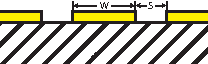
\includegraphics[width=0.9\linewidth]{figure/chipsubstrat.pdf}
  %\caption{Genomskärning av en ko-planär vågledare på ett chipsubstrat av kisel (streckad). Ledaren med bredd W är gjord av aluminium (gul) och är separerad från ett jordplan av två gap med bredd S.}
  %\label{fig:chipgenom}
\end{subfigure}%
\begin{subfigure}{.5\textwidth}
  \centering
  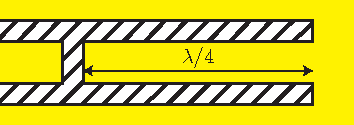
\includegraphics[width=0.9\linewidth]{figure/chipsubstrat2.pdf}
  %\caption{}
  %\label{fig:chipovan}
\end{subfigure}
\caption{Genomskärning av en ko-planär vågledare (vänster) på ett chipsubstrat av kisel (streckad). Ledaren med bredd W är gjord av aluminium (gul) och är separerad från ett jordplan av två gap med bredd S. Till höger, en kvartsvågsresonator från ovan. Ena änden är kortsluten och den andra är öppen. Figurerna är från \cite[fig. 2.1]{Boehme2016}.}
\label{fig:chipsubstrat}
\end{figure}

Den typ av resonatorer som användes i projektet är supraledande kvartvågsresonatorer som tillverkades av vår Dr. Jonathan Burnett. De består av en ko-planär vågledare på ett chipsubstrat av kisel, med en mittledare av aluminium separerad från ett jordplan \cite{Boehme2016} vilket kan ses i figur \ref{fig:chipsubstrat}. Själva resonatorerna är kortslutna i ena änden och öppna i den andra och behöver i allmänhet inte vara helt raka. I \figref{fig:chip} visas ett antal resonatorer som är etsade på ett chipp. Vi kan se en matarledning som går längsmed chippet och resonatorerna hängandes bredvid. Ett mikrovågsfält kopplas in i resonatorna via en kapacitiv koppling till denna matarledning.

Resonatorerna tillverkas med resonansfrekvenser inom \unit[4-8]{GHz} vilket motsvarar en ungefärlig längd av \unit[1-2]{cm}. På samma chipp brukar resonatorerna skapas med olika resonansfrekvenser för att kunna adressera dem separat. Vi kan visualisera detta med en mätning av amplitudspektrumet (\figref{fig:ex_wide}) för chippet, där resonatorerna manifesterar sig som smala gropar i amplituden. Uppställningen för en sådan mätning förklaras i avsnitt \ref{sec:matuppstallning}.

\tikzfig{matningar/wide_resonator_example}{Amplitudspektrum i bandet \unit[3-8]{GHz} för ett chipp med 9 resonatorer som är markerade i figuren.}{fig:ex_wide}{0.8\columnwidth}{10em}

Med denna allmänna mätuppställning undersöker vi även fasspektrumet som tillsammans med amplitudspektrumet ger resonatorernas inbördes transmissionsegenskaper och således låter oss beräkna resonansfrekvenserna och Q-värderna. Dessa två egenskaper karakteriserar resonatorerna och förklaras mer ingående i avsnitt \ref{sec:res_teori}.

\section{Mätuppställning i en kryostat}
\label{sec:matuppstallning}
\begin{figure}
    \centering
    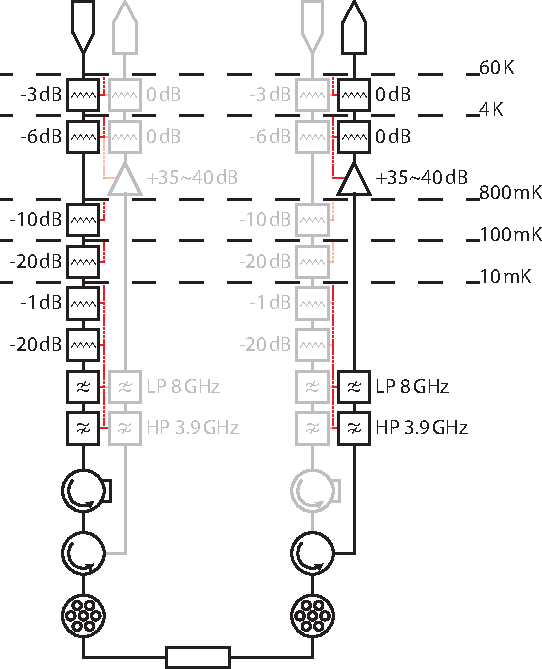
\includegraphics[width=0.7\textwidth]{figure/kretsar/cryo.pdf}
    \caption{Allmänt kretsschema för en transmissionsmätning på ett resonatorchipp.
    En mätsignal från en VNA dämpas vid varje temperatursteg och filtreras innan den når provlådan (botten). Innehållet i provlådan byts ut med switchar beroende på vilket chipp som ska mätas. Sedan förstärks signalen på väg tillbaka till analysatorn. Figuren är från \cite[fig. 3.7]{Boehme2016} (\copyright Thijs Boehme, med tillåtelse).}
    \label{fig:matuppstallning}
\end{figure}

Mätuppställningen för resonatorn visas schematiskt i \figref{fig:matuppstallning}. Hela kretsen befinner sig i en kryostat med flera nivåer för att göra temperaturgradienterna små mellan stegen. Det gör det lättare att bibehålla de låga temperaturerna.

En nätverksanalysator (VNA av modell Agilent E8364b) användes för att mäta S-parametern $S_{21}$ i frekvensbandet \unit[4-8]{GHz} vilket är resonatorernas frekvensområde.
Analysatorn skickar ett mikrovågsfält in i kretsen som först dämpas genom varje temperatursteg, med en total dämpning av ungefär \unit[67]{dB} vid \unit[10]{mK}. I varje steg sker också en termisk kortslutning av ledaren genom en termisk koppling till jord. Detta för att ledaren inte ska vara rumstemperatur nere i kryostaten och skicka in termiskt brus. Innan signalen når provlådan, som befinner sig i botten av kretsschemat, filtreras den effektivt med ett bandpassfilter i intervallet \unit[4-8]{GHz}. Signalen tar sig genom provlådan som består av ett chipp med resonatorer och fortsätter sedan till en cirkulator. Cirkulatorn hindrar termiska signaler från att propagera ner i kretsen från analysatorns ingångsport, men låter signaler från chippet propagera upp till porten. Innan signalen når analysatorn fitreras den igen och förstärks med \unit[35-40]{dB} vid \unit[4]{K}.

I uppställningen är flera provlådor parallellt kopplade och lådan som mäts kan väljas vid behov. Det är för ineffektivt att byta låda mellan varje mätning eftersom det tar flera dagar att kyla ner kryostaten.

Mätdatan består av amplitud- och fasdata över frekvens och anpassas till en teoretisk modell från vilket resonatorernas karakteristik kan bestämmas.

\section{Teoretisk modell för resonatorernas transmissionskoefficient}
\label{sec:res_teori}

\begin{figure}
\centering
\ctikzset{bipoles/thickness=1}
\begin{circuitikz}[line width=1pt,scale=0.7]
\draw

(0,5) node[label={left:$1$}] {} -- (6,5) node[label={right:$2$}] {}
(3,3) to[C] (3,5)

(1,3) -- (5,3)
(5,1) to[C] (5,3)
(3,1) to[R] (3,3)
(1,1) to[L] (1,3)
(1,1) -- (5,1)

(3,0.75) -- (3,1)
(3,0.75) node[sground]{};
\end{circuitikz}
\caption{Kretsmodell av en hängande kvartsvågsresonator. Den är kapacitivt kopplad till matarledningen och består av en parallellkopplad induktans och kapacitans. De dissipativa förlusterna modelleras som en resistans.}
\label{fig:ekviv_krets}
\end{figure}
En resonatorer definieras av dess resonansfrekvens $f_r$ och kvalitetsfaktor $Q$ \cite[s. 3]{Boehme2016} så vi är naturligt intresserade av att mäta dessa för att kunna evaluera eventuella förbättringar i resonatorerna. Kvalitetsfaktorn (eller Q-värde) är ett mått på resonatorns förmåga att lagra energi per cykel och den totala kvalitetsfaktorn $Q_l$ brukar delas upp i två delar \cite{Probst2015}: intern kvalitetsfaktor $Q_i$ och kopplad kvalitetsfaktor $Q_c$ och förhåller sig enligt 
\begin{equation}
\frac{1}{Q_l}=\frac{1}{Q_i}+\text{Re}\qty(\frac{1}{Q_c}).
\end{equation}
Detta förklaras mer ingående i avsnitt \ref{sec:losses}.

För att erhålla en modell för resonatorerna utifrån sagda parametrar krävs en ekvivalent kretsmodell. Eftersom resonatorerna är vågledare kan de modelleras med induktanser, kapacitanser och resistanser \cite[s. 437]{cheng}. En härledning av en allmän transmissionsledning finns i appendix \ref{app:trans}. Vi betraktar den ekvivalenta kretsmodellen för en hängande resonator \cite{Boehme2016} i \figref{fig:ekviv_krets}. Anledningen att resonatorerna är hängande är för att en reflektionsmätning behöver göras för att kunna bestämma interna kvalitetsfaktorn \cite{Probst2015}. När resonatorerna är hängande mäter vi reflektionen av resonatorn genom att mäta transmissionen mellan port 1 och port 2 (i \figref{fig:ekviv_krets}). Denna geometri gör även att flera resonatorer kan hängas från samma matarledning och mätas individuellt.

Transmissionen i kretsen beskrivs av den komplexa transmissionskoefficienten $S_{21}$ som härleds av \citeauthor{Boehme2016} \cite[s. 38]{Boehme2016}:
\begin{equation}
    S_{21}(f)=1-\frac{Q_l/Q_c}{1+2iQ_l\qty(f/f_r-1)}.
\label{eq:S21_ideal}
\end{equation}

Det går att visualisera $S_{21}$ med en graf av magnituden och fasen över frekvensen för en ideal resonator vilket visas i \figref{fig:ex_magphs}. Det är värt att notera hur magnituden av transmissionen har ett minimum vid resonansfrekvensen. Det förklaras av att fältet kopplar till resonatorn. Vi kan även observera en fasvändning vid resonansfrekvensen.

Det går även att visualisera $S_{21}$ i det komplexa planet där samma resonator representeras av en cirkel (se \figref{fig:ex_cmplx}). Här parametriserar frekvensen real- och imaginärdelen av $S_{21}$. Resonansfrekvensen motsvaras av punkten där cirkeln skär x-axeln och $f=\pm\infty$ motsvaras av punkten $(1,0i)$. Cirkelns diameter kommer att förhålla sig enligt $d=Q_l/|Q_c|$ och med hjälp av en anpassning till cirkeln kan resten av parametrarna även bestämmas. Att anpassa till cirkeln ger bättre noggrannhet för parametrarna i \ref{eq:S21_ideal} och fungerar bättre för lågt signal-brusförhållande \cite{Probst2015}.

Det finns två arbetsområden för en resonator: där den är underkopplad ($Q_i<Q_c$) respektive överkopplad ($Q_i>Q_c$) \cite{Boehme2016}. Dessa två visas i graferna i figur \ref{fig:ex_magphs} och \ref{fig:ex_cmplx}. När $Q_i=Q_c$ är resonatorn kritisk kopplad och detta är gränsen mellan de två områdena. Underkoppling innebär att resonatorn har stora interna förluster och fältet eller fotonerna ''försvinner'' till dissipativa förluster innan de hinner lämna resonatorn genom den kapacitiva kopplingen. I motsats innebär överkoppling att fotonerna i större grad hinner lämna resonatorn innan de försvinner. Det önskvärda området vi vill jobba med är det överkopplade eftersom vi vill undersöka ett dominerande $Q_i$.

\begin{figure}[H]
     \begin{subfigure}[b]{0.48\textwidth}
          \centering
          \setlength\figurewidth{0.75\linewidth}
          \setlength\figureheight{\figurewidth}
          % This file was created by matlab2tikz.
%
\definecolor{mycolor1}{rgb}{0.1253 0.3242 0.8303}%
\definecolor{mycolor2}{rgb}{0.1801 0.7177 0.6424}%
\definecolor{mycolor3}{rgb}{0.9990 0.7653 0.2164}%
%
\begin{tikzpicture}[%
trim axis left, trim axis right
]

\begin{axis}[%
width=\figurewidth,
height=\figureheight,
at={(0\figurewidth,0\figureheight)},
scale only axis,
xmin=98,
xmax=102,
xlabel style={font=\color{white!15!black}},
xlabel={$\text{f/f}_\text{r}\text{ [\%]}$},
ymin=0,
ymax=1,
ylabel style={font=\color{white!15!black}},
ylabel={$\text{$|$S}_{\text{21}}\text{$|$}$},
axis background/.style={fill=white},
axis x line*=bottom,
axis y line*=left,
xmajorgrids,
ymajorgrids,
legend style={at={(0.03,0.03)}, anchor=south west, legend cell align=left, align=left, draw=white!15!black,font=\tiny}
]
\addplot [color=mycolor1, line width=2.0pt]
  table[row sep=crcr]{%
98	0.999757184726803\\
98.9320932093209	0.999150439854532\\
99.2561256125613	0.998255499753057\\
99.4261426142614	0.99708277838225\\
99.5321532153215	0.995637087363662\\
99.6049604960496	0.993924107121757\\
99.6585658565857	0.991934017518602\\
99.6997699769977	0.989667529202961\\
99.7321732173217	0.987154594170349\\
99.7589758975898	0.984330903095056\\
99.7809780978098	0.9812761731271\\
99.7997799779978	0.977924593164346\\
99.8161816181618	0.974239755699841\\
99.8305830583058	0.970225718219524\\
99.8433843384339	0.965861014322797\\
99.8545854585459	0.96125697005138\\
99.8649864986499	0.956158976904547\\
99.8745874587459	0.950584211518958\\
99.8833883388339	0.944579855751073\\
99.8913891389139	0.938229091774218\\
99.8989898989899	0.931262920401963\\
99.9065906590659	0.923230872327807\\
99.9137913791379	0.914481387952478\\
99.9205920592059	0.905053892988249\\
99.9273927392739	0.894358567721611\\
99.9341934193419	0.882275262933547\\
99.9413941394139	0.867879388757942\\
99.9489948994899	0.850902062640643\\
99.957795779578	0.829259664373794\\
99.979397939794	0.77500904107599\\
99.984598459846	0.764635217939542\\
99.988598859886	0.758242640910765\\
99.992199219922	0.753929192873059\\
99.99499949995	0.751630001347635\\
99.997799779978	0.750317275769731\\
100.000200020002	0.750002625496847\\
100.002600260026	0.750442908961176\\
100.00500050005	0.751630001347635\\
100.007800780078	0.753929192873059\\
100.01100110011	0.757692229439641\\
100.014601460146	0.763234206412406\\
100.01900190019	0.771603814882766\\
100.024202420242	0.783227948987545\\
100.031803180318	0.802250681191197\\
100.050605060506	0.849960609692005\\
100.058605860586	0.867879388757942\\
100.066206620662	0.883026197678703\\
100.073407340734	0.895686795229295\\
100.080608060806	0.906805945374046\\
100.087808780878	0.916529850907565\\
100.09500950095	0.925018747772342\\
100.102610261026	0.932812578110287\\
100.110611061106	0.939904973486478\\
100.11901190119	0.946312039505344\\
100.127812781278	0.952065965917413\\
100.137413741374	0.957415256164509\\
100.147814781478	0.962314349621934\\
100.15901590159	0.966745911394298\\
100.171417141714	0.970834770712386\\
100.185418541854	0.974636881781251\\
100.201420142014	0.978163615904023\\
100.219421942194	0.981339212964826\\
100.240624062406	0.984282090296148\\
100.265426542654	0.986933618568315\\
100.295429542954	0.989343681588252\\
100.331833183318	0.991476932053246\\
100.377837783778	0.993373536273438\\
100.43704370437	0.995013332525602\\
100.516651665167	0.99641095967506\\
100.629062906291	0.997567485549368\\
100.798679867987	0.998485275353346\\
101.082308230823	0.999172822689459\\
101.63796379638	0.999638159908955\\
102	0.999757184726803\\
};
\addlegendentry{$\textit{Q}_\textit{i}\text{\textless{}}\textit{Q}_\textit{c}$}

\addplot [color=mycolor2, dashed, line width=2.0pt]
  table[row sep=crcr]{%
98	0.999064400231774\\
98.5832583258326	0.998139216594751\\
98.8972897289729	0.996936504936187\\
99.0953095309531	0.995463264685469\\
99.2325232523252	0.99372006198891\\
99.3337333733373	0.991704061218485\\
99.4113411341134	0.989425726557954\\
99.4729472947295	0.98688339615434\\
99.5233523352335	0.984063097247301\\
99.5653565356536	0.980966585397724\\
99.6005600560056	0.97763278019444\\
99.6309630963096	0.974010411821794\\
99.6573657365737	0.970118283657214\\
99.6805680568057	0.965949113304376\\
99.7013701370137	0.961446701098708\\
99.7197719771977	0.956703087050229\\
99.7365736573657	0.95159537333781\\
99.7517751775178	0.946189282942498\\
99.7657765776578	0.940408112358568\\
99.7785778577858	0.934313196471678\\
99.7905790579058	0.92776218659715\\
99.8017801780178	0.920783746213047\\
99.8121812181218	0.913427030115955\\
99.8221822182218	0.90542506711779\\
99.8317831783178	0.896750628620495\\
99.8409840984098	0.887384616077625\\
99.8497849784979	0.877318769250508\\
99.8581858185819	0.866558571469881\\
99.8665866586659	0.854521669532701\\
99.8745874587459	0.84171982716407\\
99.8825882588259	0.827455176361923\\
99.8905890589059	0.811564608744263\\
99.8985898589859	0.79388333407779\\
99.9065906590659	0.774256080370535\\
99.9145914591459	0.752555046898635\\
99.9229922992299	0.727458386200183\\
99.9317931793179	0.698663324238709\\
99.9417941794179	0.663169196311756\\
99.95699569957	0.605850600092424\\
99.968596859686	0.563314045270857\\
99.975397539754	0.541114741381122\\
99.980598059806	0.526505864283507\\
99.98499849985	0.516243059084545\\
99.988598859886	0.509532975458669\\
99.991799179918	0.504985457879769\\
99.994599459946	0.50217633972072\\
99.99699969997	0.500674073448764\\
99.999399939994	0.500027003699259\\
100.001800180018	0.500242910863619\\
100.004200420042	0.501319193773739\\
100.006600660066	0.503242961710129\\
100.009400940094	0.50652764897491\\
100.012601260126	0.511588923436449\\
100.016201620162	0.5188288616297\\
100.020202020202	0.528591412607327\\
100.02500250025	0.542333801920194\\
100.03100310031	0.561932256976831\\
100.039403940394	0.592283255485654\\
100.068206820682	0.698663324238709\\
100.077407740774	0.728707270294066\\
100.085808580858	0.753690783037442\\
100.094209420942	0.776310339212486\\
100.102210221022	0.795736611903223\\
100.110211021102	0.813231556948807\\
100.118211821182	0.828952075548884\\
100.126212621262	0.843063202400415\\
100.134613461346	0.856325494880764\\
100.14301430143	0.868170246339488\\
100.151815181518	0.879236223375869\\
100.160616061606	0.88909407557432\\
100.169816981698	0.898270115746513\\
100.179417941794	0.906772362942718\\
100.189418941894	0.914619277958153\\
100.200220022002	0.922097449950527\\
100.211421142114	0.928916424461747\\
100.223422342234	0.935322392652026\\
100.236223622362	0.941286889420709\\
100.250225022502	0.946948830007798\\
100.265426542654	0.952247783923141\\
100.281828182818	0.957148279254227\\
100.299829982998	0.96172939850436\\
100.319831983198	0.966028023222947\\
100.342234223422	0.970052889349205\\
100.367436743674	0.973796356338895\\
100.396239623962	0.977287772719933\\
100.429442944294	0.98052229365382\\
100.467846784678	0.98347944820938\\
100.513451345135	0.986200260326271\\
100.567856785679	0.98865615121089\\
100.634263426343	0.990862717561058\\
100.717071707171	0.992820356800436\\
100.823482348235	0.994535463710434\\
100.964696469647	0.996005371022974\\
101.160716071607	0.997233256816827\\
101.450345034503	0.998224115701305\\
101.917191719172	0.998982015093219\\
102	0.999064400231774\\
};
\addlegendentry{$\textit{Q}_\textit{i}\text{=}\textit{Q}_\textit{c}$}

\addplot [color=mycolor3, dashdotted, line width=2.0pt]
  table[row sep=crcr]{%
98	0.995348090761311\\
98.2992299229923	0.993585826430191\\
98.5200520052005	0.991557215625747\\
98.6900690069007	0.989264203498124\\
98.8256825682568	0.986698199957203\\
98.9360936093609	0.98387021272822\\
99.028102810281	0.980771560646701\\
99.1057105710571	0.977417026073155\\
99.1725172517252	0.973784590042186\\
99.2305230523052	0.969883216378477\\
99.2813281328133	0.965719034637232\\
99.3265326532653	0.961260177482799\\
99.3665366536654	0.956566325617871\\
99.4025402540254	0.951594242735226\\
99.4353435343534	0.946306348068958\\
99.4649464946495	0.940780970013833\\
99.4921492149215	0.934946030411197\\
99.5173517351735	0.928769008755083\\
99.5405540554055	0.922307705457371\\
99.5621562156216	0.915509584143351\\
99.5821582158216	0.90843248407036\\
99.6009600960096	0.900987248979433\\
99.6185618561856	0.893217934992094\\
99.6353635363536	0.884978277363899\\
99.6513651365136	0.87628098281273\\
99.6665666566657	0.867149178340469\\
99.6809680968097	0.857617771103591\\
99.6949694969497	0.847429955407165\\
99.7081708170817	0.836895295344064\\
99.7209720972097	0.825721888228728\\
99.7333733373337	0.81390121386795\\
99.7453745374537	0.801431253121308\\
99.7573757375738	0.787845649411082\\
99.7689768976898	0.773549783650822\\
99.7801780178018	0.758561665072079\\
99.7913791379138	0.742307260211476\\
99.8025802580258	0.724681663487686\\
99.8137813781378	0.705577689123828\\
99.8245824582458	0.685656104212569\\
99.8353835383538	0.664169260039031\\
99.8465846584658	0.640145225957028\\
99.8577857785779	0.614275021842147\\
99.8693869386939	0.585486487617075\\
99.8813881388139	0.553569205178988\\
99.8937893789379	0.518392394225344\\
99.9077907790779	0.476282081837439\\
99.9257925792579	0.419459494902696\\
99.950595059506	0.341199767027049\\
99.960596059606	0.312299420506434\\
99.968196819682	0.292610728617603\\
99.974197419742	0.279013603896416\\
99.979397939794	0.268967426751047\\
99.983798379838	0.261939036101751\\
99.987798779878	0.256858322374185\\
99.991399139914	0.253437534217184\\
99.994599459946	0.251362439807323\\
99.997799779978	0.250226790054811\\
100.000600060006	0.250016877653863\\
100.003400340034	0.250541240888595\\
100.006200620062	0.251794067441864\\
100.009400940094	0.25409995141213\\
100.01300130013	0.257769390346652\\
100.01700170017	0.263108696124348\\
100.021402140214	0.270396079959113\\
100.026202620262	0.279857307239112\\
100.031803180318	0.292610728617603\\
100.038603860386	0.310118319983829\\
100.04700470047	0.334025725063782\\
100.058205820582	0.36838035053556\\
100.106210621062	0.518392394225344\\
100.119411941194	0.555763541758196\\
100.131813181318	0.588559240432403\\
100.143414341434	0.617136809389805\\
100.15501550155	0.643688785438727\\
100.166216621662	0.667454615718995\\
100.177417741774	0.689460740896806\\
100.188618861886	0.709801233935721\\
100.199819981998	0.728579366250955\\
100.21102110211	0.745902154156752\\
100.222622262226	0.762423391931577\\
100.234223422342	0.77761374123989\\
100.245824582458	0.791583586719369\\
100.257825782578	0.804861345175851\\
100.270227022702	0.817439954923998\\
100.28302830283	0.829320957754817\\
100.296229622962	0.84051323431315\\
100.309830983098	0.851031756711706\\
100.323832383238	0.860896400226892\\
100.338633863386	0.870375128430354\\
100.353835383538	0.879205155194967\\
100.369836983698	0.887621092951235\\
100.386638663866	0.895600249530688\\
100.404640464046	0.903291968567473\\
100.423442344234	0.910496586385193\\
100.443444344434	0.917351281238112\\
100.46504650465	0.923942075597935\\
100.488248824882	0.93021255255141\\
100.513051305131	0.93612397075448\\
100.540254025403	0.941809667346263\\
100.569856985699	0.94719912754725\\
100.602260226023	0.952303832001292\\
100.637863786379	0.957122257907912\\
100.677067706771	0.961645647463669\\
100.720672067207	0.965898587999263\\
100.769876987699	0.969912983016059\\
100.825482548255	0.97366282046768\\
100.888688868887	0.977142077495358\\
100.961496149615	0.98036663403974\\
101.046304630463	0.983337770956922\\
101.146314631463	0.986055295204693\\
101.265926592659	0.988519056296397\\
101.411941194119	0.99073689512413\\
101.59395939594	0.992707960931213\\
101.827182718272	0.994434873294892\\
102	0.995348090761311\\
};
\addlegendentry{$\textit{Q}_\textit{i}\text{\textgreater{}}\textit{Q}_\textit{c}$}

\end{axis}
\end{tikzpicture}%
     \end{subfigure}
     \begin{subfigure}[b]{0.48\textwidth}
          \centering
          \setlength\figurewidth{0.75\linewidth}
          \setlength\figureheight{\figurewidth}
          % This file was created by matlab2tikz.
%
\definecolor{mycolor1}{rgb}{0.00000,0.44700,0.74100}%
\definecolor{mycolor2}{rgb}{0.85000,0.32500,0.09800}%
\definecolor{mycolor3}{rgb}{0.92900,0.69400,0.12500}%
%
\begin{tikzpicture}[%
trim axis left, trim axis right
]

\begin{axis}[%
width=\figurewidth,
height=\figureheight,
at={(0\figurewidth,0\figureheight)},
scale only axis,
xmin=98,
xmax=102,
xlabel style={font=\color{white!15!black}},
xlabel={$\text{f/f}_\text{r}\text{ [\%]}$},
ymin=-45,
ymax=45,
ylabel style={font=\color{white!15!black}},
ylabel={$\angle\text{ S}_{\text{21}}\text{ [}^\text{o}\text{]}$},
axis background/.style={fill=white},
axis x line*=bottom,
axis y line*=left,
xmajorgrids,
ymajorgrids,
legend style={at={(0.60,0.03)}, anchor=south west, legend cell align=left, align=left, draw=white!15!black}
]
\addplot [color=mycolor1, line width=2.0pt]
  table[row sep=crcr]{%
98	-0.47705624883173\\
98.0972097209721	-0.50138313418617\\
98.1880188018802	-0.526459274016077\\
98.2728272827283	-0.552251819460423\\
98.3520352035204	-0.578729951939025\\
98.4264426442644	-0.606021942588455\\
98.4960496049605	-0.633987349601497\\
98.5616561656166	-0.662811620552418\\
98.6236623662366	-0.692566858905124\\
98.6820682068207	-0.723140590210988\\
98.7372737273727	-0.754623084511536\\
98.7896789678968	-0.787147936612016\\
98.8396839683968	-0.820902252822947\\
98.8872887288729	-0.855832825316327\\
98.9324932493249	-0.891861019711385\\
98.975697569757	-0.929239186620464\\
99.017301730173	-0.968307619873201\\
99.0573057305731	-1.00908942560017\\
99.0953095309531	-1.05113257742042\\
99.1321132113211	-1.09531165417569\\
99.1673167316732	-1.14117235957491\\
99.2013201320132	-1.18924886306048\\
99.2341234123412	-1.23960638183809\\
99.2661266126613	-1.29299500247252\\
99.2969296929693	-1.34888080071975\\
99.3269326932693	-1.40812620772384\\
99.3561356135613	-1.47096896729218\\
99.3845384538454	-1.53766295791876\\
99.4121412141214	-1.60847852647611\\
99.4385438543854	-1.68252868997958\\
99.4645464546455	-1.76235158000144\\
99.4897489748975	-1.84719193225288\\
99.5141514151415	-1.93738057936129\\
99.5381538153815	-2.03496520446751\\
99.5613561356136	-2.1389375616959\\
99.5841584158416	-2.25178992747736\\
99.6061606160616	-2.37230082687933\\
99.6277627762776	-2.50351958982357\\
99.6485648564856	-2.64394211971883\\
99.6689668966897	-2.79731329234298\\
99.6889688968897	-2.96529112204365\\
99.7085708570857	-3.14978980555016\\
99.7273727372737	-3.34853049793189\\
99.7457745774578	-3.56738815542437\\
99.7637763776378	-3.80899274631481\\
99.7813781378138	-4.07629236860507\\
99.7985798579858	-4.37251999975935\\
99.8157815781578	-4.70942907393228\\
99.8325832583258	-5.08427072679115\\
99.8493849384939	-5.51086661743152\\
99.8665866586659	-6.00655756209477\\
99.8857885788579	-6.62959330567013\\
99.9265926592659	-7.98494211922522\\
99.9337933793379	-8.1378524523231\\
99.9385938593859	-8.19784141220173\\
99.9413941394139	-8.2123029658531\\
99.9425942594259	-8.21307818737233\\
99.9441944194419	-8.20853313622189\\
99.9461946194619	-8.19312426505834\\
99.9489948994899	-8.1513769972032\\
99.952595259526	-8.05823488970505\\
99.95699569957	-7.87373762805622\\
99.961796179618	-7.56741119859133\\
99.967396739674	-7.04607745269608\\
99.973397339734	-6.2613814982975\\
99.980198019802	-5.06254383807702\\
99.988598859886	-3.14045019965671\\
100.001800180018	0.51519881421963\\
100.015801580158	4.20379952601773\\
100.024602460246	5.94353399051991\\
100.031803180318	6.95558641857249\\
100.038203820382	7.56741119859133\\
100.043804380438	7.91365633146503\\
100.04900490049	8.10551801165035\\
100.05300530053	8.18370687569544\\
100.056205620562	8.21029199450373\\
100.057805780578	8.21320462593044\\
100.059405940594	8.20991473492104\\
100.061406140614	8.19784141220173\\
100.064606460646	8.16225273014545\\
100.069406940694	8.07775850055164\\
100.076207620762	7.91056167832893\\
100.086608660866	7.58888558027175\\
100.114211421142	6.62959330567013\\
100.135413541354	5.94577487541017\\
100.153815381538	5.42534355273942\\
100.171417141714	4.99056440355058\\
100.18901890189	4.61093464841487\\
100.206620662066	4.27896563770253\\
100.224622462246	3.98138935038244\\
100.24302430243	3.71422579304219\\
100.261826182618	3.47380811140599\\
100.28102810281	3.25686494921911\\
100.300630063006	3.06052777508368\\
100.32103210321	2.87894349120099\\
100.341834183418	2.71403492360862\\
100.36303630363	2.56379841665333\\
100.38503850385	2.42410556881113\\
100.407440744074	2.29636193086577\\
100.430643064306	2.17724921352938\\
100.454245424542	2.06791354983915\\
100.478647864786	1.96567449188923\\
100.503450345035	1.87148342856533\\
100.529052905291	1.78316080699386\\
100.555455545555	1.70030822364006\\
100.582258225823	1.6236420588173\\
100.609860986099	1.55152736804688\\
100.638663866387	1.48274815471838\\
100.668266826683	1.41808804658631\\
100.698669866987	1.35725846583762\\
100.729872987299	1.2999915561338\\
100.761876187619	1.24603905238872\\
100.795079507951	1.19457623233019\\
100.829482948295	1.14553170959566\\
100.865086508651	1.09882491807197\\
100.901890189019	1.05436891215409\\
100.939893989399	1.01207267432413\\
100.979497949795	0.971448904420242\\
101.021102110211	0.932132548235217\\
101.064306430643	0.89452665837635\\
101.109510951095	0.858287745086798\\
101.156715671567	0.823444340333495\\
101.206320632063	0.7897460362001\\
101.258325832583	0.757250672300302\\
101.313131313131	0.725773747719174\\
101.370737073707	0.695386271563464\\
101.431543154315	0.665949884908642\\
101.49594959496	0.637367772116747\\
101.56395639564	0.60973187154751\\
101.636363636364	0.58282246664568\\
101.713571357136	0.556625106087282\\
101.795579557956	0.531258030156025\\
101.883188318832	0.50659197107727\\
101.977197719772	0.482548380701459\\
102	0.47705624883173\\
};
\addlegendentry{$\text{Q}_\text{i}\text{\textless{}Q}_\text{c}$}

\addplot [color=mycolor2, dashed, line width=2.0pt]
  table[row sep=crcr]{%
98	-1.4303090419471\\
98.0624062406241	-1.47623595103011\\
98.1224122412241	-1.52326171819043\\
98.1804180418042	-1.57165314001921\\
98.2364236423642	-1.6213799658328\\
98.2908290829083	-1.67278846386006\\
98.3436343634363	-1.72589463560234\\
98.3944394439444	-1.78026479359802\\
98.4436443644364	-1.83628258526717\\
98.4916491649165	-1.89443004161163\\
98.5384538453845	-1.95477235757825\\
98.5836583658366	-2.01680572560267\\
98.6280628062806	-2.0816854257189\\
98.6712671267127	-2.14893392521414\\
98.7132713271327	-2.21859977235415\\
98.7544754475447	-2.29145436736842\\
98.7944794479448	-2.36689641311629\\
98.8336833683368	-2.44578833262962\\
98.8720872087209	-2.52831720650161\\
98.9096909690969	-2.6146802416051\\
98.946494649465	-2.70508506730404\\
98.982498249825	-2.79974997034174\\
99.017301730173	-2.89773810317557\\
99.0513051305131	-3.00028742910854\\
99.0849084908491	-3.10896732171067\\
99.1177117711771	-3.22287267519293\\
99.1497149714971	-3.3422732977611\\
99.1813181318132	-3.46911331032773\\
99.2121212121212	-3.60227079463624\\
99.2425242524252	-3.74400967961144\\
99.2721272127213	-3.89303799895329\\
99.3013301330133	-4.0520043989049\\
99.3297329732973	-4.21941192914203\\
99.3577357735774	-4.39837384377138\\
99.3849384938494	-4.58714351902459\\
99.4117411741174	-4.78939712605194\\
99.4377437743774	-5.00308021520669\\
99.4633463346335	-5.23255248320548\\
99.4885488548855	-5.47947146245127\\
99.5129512951295	-5.74122354295156\\
99.5369536953695	-6.0235534553446\\
99.5605560556056	-6.32872588966767\\
99.5833583358336	-6.65333337628704\\
99.6057605760576	-7.00502852253045\\
99.6277627762776	-7.38689103574779\\
99.6493649364937	-7.80240680928804\\
99.6705670567057	-8.25551199945943\\
99.6909690969097	-8.74058816829123\\
99.7109710971097	-9.27027542932086\\
99.7309730973097	-9.86202691336561\\
99.7505750575058	-10.5116122462901\\
99.7697769776978	-11.2250153769657\\
99.7889788978898	-12.0256182193462\\
99.8081808180818	-12.9243792570281\\
99.8277827782778	-13.9524562651616\\
99.8485848584859	-15.1680547290935\\
99.8749874987499	-16.8575794863783\\
99.9013901390139	-18.5137992328499\\
99.9121912191219	-19.0560122976685\\
99.9193919391939	-19.317664673772\\
99.9245924592459	-19.43404031197\\
99.9277927792779	-19.4672722176136\\
99.9293929392939	-19.4712012735231\\
99.9305930593059	-19.4681030327363\\
99.9325932593259	-19.4506224675923\\
99.9353935393539	-19.398052425151\\
99.9389938993899	-19.2765525577035\\
99.9433943394339	-19.0333967972001\\
99.948194819482	-18.6293491643404\\
99.953795379538	-17.94167048988\\
99.959795979598	-16.8999695948262\\
99.966596659666	-15.2745288390749\\
99.973797379738	-12.9739898469541\\
99.982198219822	-9.5036114866122\\
99.99299929993	-3.96582509744343\\
100.020602060206	10.7524464876108\\
100.029802980298	14.2018371864734\\
100.037803780378	16.3835496598516\\
100.04500450045	17.7601719935583\\
100.051405140514	18.5883858910948\\
100.057405740574	19.0860644356664\\
100.062606260626	19.3385176198527\\
100.066606660666	19.4390750674864\\
100.069406940694	19.4681030327363\\
100.070607060706	19.4712012735231\\
100.071807180718	19.4690889846275\\
100.073807380738	19.4546913217134\\
100.076607660766	19.4135891056369\\
100.080608060806	19.317664673772\\
100.086208620862	19.1225922634472\\
100.094209420942	18.7514896876598\\
100.105810581058	18.0900905173279\\
100.127812781278	16.6741287045977\\
100.158215821582	14.7570658770017\\
100.179817981798	13.5401534038589\\
100.200220022002	12.5184328549384\\
100.220222022202	11.6304085230935\\
100.240224022402	10.8432725636219\\
100.260226022602	10.1445374415798\\
100.280628062806	9.51071821544474\\
100.301430143014	8.93512358806608\\
100.322632263226	8.41149813345055\\
100.344234423442	7.93415806914952\\
100.366236623662	7.49802295348269\\
100.388638863886	7.09859455818176\\
100.411441144114	6.73191121327517\\
100.43504350435	6.38896196581244\\
100.45904590459	6.07325078496623\\
100.483448344834	5.78191881345622\\
100.508650865087	5.50831887819706\\
100.534253425343	5.25512631352274\\
100.560256025603	5.02029457502674\\
100.587058705871	4.79886393721765\\
100.614261426143	4.59293725140476\\
100.642264226423	4.39837384377138\\
100.670667066707	4.2169593687986\\
100.699469946995	4.04747849184525\\
100.729072907291	3.88676853119961\\
100.759075907591	3.73627510349279\\
100.789878987899	3.59331759006717\\
100.821482148215	3.4574903052375\\
100.853485348535	3.32993981605581\\
100.886288628863	3.20854025588258\\
100.919491949195	3.09429265234306\\
100.953495349535	2.98537489155925\\
100.988298829883	2.88151221294511\\
101.023902390239	2.78244211406367\\
101.060306030603	2.68791440335202\\
101.097509750975	2.59769110229158\\
101.135513551355	2.51154623150792\\
101.174317431743	2.42926550917164\\
101.213921392139	2.35064598489558\\
101.254725472547	2.27477549096032\\
101.296329632963	2.20228223120156\\
101.338733873387	2.13298479435271\\
101.382338233823	2.06611795131002\\
101.427142714271	2.00162933024127\\
101.473147314731	1.93946116035045\\
101.520352035204	1.87955151654894\\
101.568756875688	1.82183539792892\\
101.618761876188	1.76581110674391\\
101.6699669967	1.71189665189588\\
101.722772277228	1.65963371813244\\
101.777577757776	1.60865611424229\\
101.83398339834	1.55935454255011\\
101.892389238924	1.51138628625907\\
101.952795279528	1.46477942997639\\
102	1.4303090419471\\
};
\addlegendentry{$\text{Q}_\text{i}\text{=Q}_\text{c}$}

\addplot [color=mycolor3, dashdotted, line width=2.0pt]
  table[row sep=crcr]{%
98	-4.27849695333499\\
98.0500050005001	-4.3872240187484\\
98.0992099209921	-4.49971705866314\\
98.1476147614761	-4.61612601750095\\
98.1952195219522	-4.73660631440686\\
98.2420242024202	-4.86131886598592\\
98.2880288028803	-4.99043007308801\\
98.3332333233323	-5.12411176464234\\
98.3780378037804	-5.2638219773538\\
98.4220422042204	-5.40860329288064\\
98.4652465246525	-5.55865642161812\\
98.5076507650765	-5.71418789614293\\
98.5496549654965	-5.87700376710652\\
98.5908590859086	-6.04591042716105\\
98.6316631663166	-6.2229329703251\\
98.6716671667167	-6.40674210230488\\
98.7112711271127	-6.59961481754092\\
98.7500750075008	-6.80006596098902\\
98.7880788078808	-7.00840286574672\\
98.8256825682568	-7.22733914137727\\
98.8628862886289	-7.45764769701078\\
98.8992899289929	-7.69745549339828\\
98.9352935293529	-7.95005193978443\\
98.970497049705	-8.21332068732187\\
99.005300530053	-8.49100233189201\\
99.039303930393	-8.78069489424472\\
99.0729072907291	-9.0866636923739\\
99.1061106110611	-9.41020115439271\\
99.1385138513851	-9.74840726709797\\
99.1705170517052	-10.1065418648526\\
99.2021202120212	-10.4862489520169\\
99.2329232923292	-10.8839850313368\\
99.2633263326333	-11.3062872864772\\
99.2933293329333	-11.7552498849213\\
99.3229322932293	-12.2331848844711\\
99.3517351735174	-12.7353929504825\\
99.3801380138014	-13.2707523720993\\
99.4081408140814	-13.8421915468515\\
99.4357435743574	-14.4529311315197\\
99.4629462946295	-15.1065064038326\\
99.4897489748975	-15.8067861484553\\
99.5161516151615	-16.5579845816489\\
99.5421542154215	-17.3646609136086\\
99.5677567756776	-18.2316982679757\\
99.5929592959296	-19.1642493520889\\
99.6177617761776	-20.167629772463\\
99.6425642564256	-21.2656439141834\\
99.6669666966697	-22.4481859128499\\
99.6913691369137	-23.7418800967855\\
99.7161716171617	-25.1796073313994\\
99.7417741774177	-26.7998378014364\\
99.7689768976898	-28.671115061327\\
99.8013801380138	-31.0684916433795\\
99.8525852585258	-34.8711862224987\\
99.8673867386739	-35.7947240099804\\
99.8781878187819	-36.3394597327457\\
99.8861886188619	-36.6406541505548\\
99.8921892189219	-36.7922238326836\\
99.8965896589659	-36.8544376547271\\
99.8993899389939	-36.8693889785036\\
99.9009900990099	-36.8685362051094\\
99.9025902590259	-36.8604282524275\\
99.9049904990499	-36.8338820511309\\
99.9081908190819	-36.7696468989712\\
99.9121912191219	-36.638402495827\\
99.9169916991699	-36.3968890506269\\
99.9225922592259	-35.9819942592547\\
99.9285928592859	-35.3515231898269\\
99.9349934993499	-34.4283310394948\\
99.9417941794179	-33.1102085079339\\
99.9489948994899	-31.2632069635852\\
99.956595659566	-28.7162659956333\\
99.96499649965	-25.0674936445519\\
99.973797379738	-20.192907722168\\
99.983798379838	-13.3226952318019\\
99.997399739974	-2.23211897465795\\
100.019401940194	15.6672772588319\\
100.030203020302	22.5468736743077\\
100.039803980398	27.2666548436959\\
100.048604860486	30.5299251999814\\
100.05700570057	32.8367664617985\\
100.06500650065	34.4283310394948\\
100.072207220722	35.447863549247\\
100.07900790079	36.1164256788084\\
100.08500850085	36.5094043635987\\
100.090209020902	36.7242642852422\\
100.094609460946	36.8277049775046\\
100.097809780978	36.8631545625496\\
100.099809980998	36.8698479003826\\
100.101410141014	36.8672014568853\\
100.103410341034	36.8544376547271\\
100.106610661066	36.8136047508998\\
100.11101110111	36.7202352230109\\
100.116611661166	36.5469462589034\\
100.123812381238	36.249257331079\\
100.133413341334	35.7493194417526\\
100.146214621462	34.9516731249348\\
100.164616461646	33.6473664725833\\
100.258225822582	26.7998378014364\\
100.28502850285	25.1070813196727\\
100.310631063106	23.6314366768549\\
100.335833583358	22.3070175096861\\
100.36103610361	21.0999961192069\\
100.386238623862	19.999654114604\\
100.411841184118	18.9801507334227\\
100.437843784378	18.0354317118576\\
100.463846384638	17.1722026789531\\
100.490249024903	16.3698922749493\\
100.517051705171	15.6234451233244\\
100.544254425443	14.9281672075091\\
100.571857185719	14.2797395036281\\
100.600260026003	13.6659149069708\\
100.629062906291	13.0926855187114\\
100.658265826583	12.5565992544804\\
100.687868786879	12.0545344491061\\
100.718271827183	11.5776316244106\\
100.749074907491	11.1302609050621\\
100.780278027803	10.7099979370777\\
100.811881188119	10.3146554281593\\
100.844284428443	9.93776882124479\\
100.877087708771	9.58265320941541\\
100.910291029103	9.24761233425824\\
100.944294429443	8.92747165776665\\
100.978697869787	8.62495433259822\\
101.013901390139	8.33555855333155\\
101.049504950495	8.06167037452252\\
101.085508550855	7.80215260177681\\
101.122312231223	7.55335188186534\\
101.159515951595	7.31726484744141\\
101.197519751975	7.0906846936138\\
101.235923592359	6.87538146049998\\
101.275127512751	6.66853155983974\\
101.314731473147	6.47171042286752\\
101.355135513551	6.2824241660163\\
101.395939593959	6.10208013182718\\
101.437543754375	5.92846888992771\\
101.479947994799	5.76131866788943\\
101.522752275228	5.60181563890012\\
101.566356635664	5.44809966680019\\
101.610761076108	5.29993997092252\\
101.655565556556	5.15834388772436\\
101.701170117012	5.02173740709766\\
101.747574757476	4.88992470558769\\
101.794779477948	4.76271672594733\\
101.842784278428	4.63993117817269\\
101.891589158916	4.52139249580938\\
101.941194119412	4.40693175550366\\
101.991599159916	4.29638656668648\\
102	4.27849695333499\\
};
\addlegendentry{$\text{Q}_\text{i}\text{\textgreater{}Q}_\text{c}$}

\end{axis}
\end{tikzpicture}%
     \end{subfigure}
   \caption{Magnitud och fas över frekvens för de olika kopplingsområdena. Vid resonansfrekvensen sjunker magnituden och en fasvändning sker. Figurerna är baserade på \cite[fig. 2.4(a-c)]{Boehme2016}.}
    \label{fig:ex_magphs}
 \end{figure}
 
\begin{figure}[H]
  \centering
  \setlength\figurewidth{14em}
  \setlength\figureheight{\figurewidth}
  % This file was created by matlab2tikz.
%
\definecolor{mycolor1}{rgb}{0.1253 0.3242 0.8303}%
\definecolor{mycolor2}{rgb}{0.1801 0.7177 0.6424}%
\definecolor{mycolor3}{rgb}{0.9990 0.7653 0.2164}%
%
\begin{tikzpicture}[%
trim axis left, trim axis right
]


\begin{axis}[%
width=\figurewidth,
height=\figureheight,
at={(0\figurewidth,0\figureheight)},
scale only axis,
xmin=-1,
xmax=1,
xlabel style={font=\color{white!15!black}},
xlabel={$\text{Re(S}_{\text{21}}\text{)}$},
ymin=-1,
ymax=1,
ylabel style={font=\color{white!15!black}},
ylabel={$\text{Im(S}_{\text{21}}\text{)}$},
axis background/.style={fill=white},
axis x line*=bottom,
axis y line*=left,
xmajorgrids,
ymajorgrids,
legend style={at={(0.03,0.97)}, anchor=north west, legend cell align=left, align=left, draw=white!15!black,legend pos = south west, font = \tiny}
]
\addplot [color=mycolor1, line width=2.0pt]
  table[row sep=crcr]{%
0.999843782549371	0.00624739615883474\\
0.998076345672995	0.0218452085314271\\
0.99436792130311	0.0370985089157838\\
0.988776993507336	0.0517667436529635\\
0.98139173455687	0.0656185859187823\\
0.9723286143971	0.0784355838860187\\
0.961730563846992	0.0900156058402259\\
0.949764720494689	0.100176027917616\\
0.936619792837906	0.108756614192488\\
0.922503084238189	0.115622043693491\\
0.907637223623069	0.120664044496187\\
0.892256654494881	0.123803101235972\\
0.876603937616682	0.124989709112878\\
0.860925925684123	0.12420515461184\\
0.84546987031097	0.121461810626011\\
0.830479522723457	0.116802941328842\\
0.816191289657839	0.110302019872221\\
0.802830505084938	0.102061569670982\\
0.790607876558813	0.0922115475474061\\
0.779716162232768	0.0809072942344987\\
0.770327130948117	0.0683270845598385\\
0.762588853336955	0.0546693159450476\\
0.756623366659834	0.0401493795599371\\
0.75252475020526	0.0249962634750897\\
0.750357641603117	0.00944894138319596\\
0.750156217450629	-0.00624739615883485\\
0.751923654327005	-0.0218452085314271\\
0.75563207869689	-0.0370985089157838\\
0.761223006492664	-0.0517667436529635\\
0.768608265443131	-0.0656185859187823\\
0.7776713856029	-0.0784355838860187\\
0.788269436153008	-0.0900156058402259\\
0.800235279505311	-0.100176027917616\\
0.813380207162094	-0.108756614192488\\
0.827496915761811	-0.115622043693491\\
0.842362776376931	-0.120664044496187\\
0.857743345505119	-0.123803101235972\\
0.873396062383318	-0.124989709112878\\
0.889074074315877	-0.12420515461184\\
0.90453012968903	-0.121461810626011\\
0.919520477276543	-0.116802941328842\\
0.933808710342161	-0.110302019872221\\
0.947169494915062	-0.102061569670982\\
0.959392123441187	-0.092211547547406\\
0.970283837767232	-0.0809072942344987\\
0.979672869051883	-0.0683270845598384\\
0.987411146663045	-0.0546693159450476\\
0.993376633340166	-0.0401493795599371\\
0.99747524979474	-0.0249962634750897\\
0.999642358396883	-0.00944894138319585\\
};
\addlegendentry{$\textit{Q}_\textit{i}\text{\textless{}}\textit{Q}_\textit{c}$}

\addplot [color=mycolor2, dashed, line width=2.0pt]
  table[row sep=crcr]{%
0.999687565098742	0.0124947923176696\\
0.998410309223681	0.0281481486317537\\
0.996152691345989	0.0436904170628541\\
0.992923621252023	0.0590602593780605\\
0.98873584260622	0.0741970178315675\\
0.983605882657683	0.0890409545530865\\
0.977553987014672	0.103533487305927\\
0.970604039744442	0.117617420684322\\
0.962783469113739	0.131237171837565\\
0.954123139341965	0.144338989830125\\
0.944657228794199	0.156871167772037\\
0.934423095094812	0.168784246882373\\
0.923461127693983	0.180031211680452\\
0.911814588468997	0.190567675534465\\
0.899529440989378	0.200352055835233\\
0.886654169119677	0.209345738103766\\
0.873239585675812	0.217513228384975\\
0.859338631890095	0.22482229332609\\
0.845006168476378	0.231244087386982\\
0.830298759119874	0.236753266680332\\
0.815274447246138	0.241328088992374\\
0.799992526950179	0.24495049958948\\
0.784513308989761	0.247606202471944\\
0.768897882766392	0.249284716793765\\
0.753207875233365	0.249979418225756\\
0.73750520768233	0.249687565098742\\
0.721851851368246	0.248410309223681\\
0.706309582937146	0.246152691345989\\
0.690939740621939	0.242923621252023\\
0.675802982168432	0.23873584260622\\
0.660959045446914	0.233605882657683\\
0.646466512694073	0.227553987014672\\
0.632382579315678	0.220604039744442\\
0.618762828162435	0.212783469113739\\
0.605661010169875	0.204123139341965\\
0.593128832227963	0.1946572287942\\
0.581215753117627	0.184423095094812\\
0.569968788319548	0.173461127693983\\
0.559432324465535	0.161814588468997\\
0.549647944164767	0.149529440989378\\
0.540654261896234	0.136654169119677\\
0.532486771615025	0.123239585675812\\
0.525177706673911	0.109338631890095\\
0.518755912613018	0.0950061684763781\\
0.513246733319668	0.0802987591198743\\
0.508671911007626	0.0652744472461378\\
0.50504950041052	0.0499925269501793\\
0.502393797528056	0.0345133089897613\\
0.500715283206235	0.0188978827663918\\
0.500020581774244	0.00320787523336474\\
0.500312434901258	-0.0124947923176696\\
0.501589690776319	-0.0281481486317537\\
0.503847308654011	-0.0436904170628543\\
0.507076378747977	-0.0590602593780605\\
0.51126415739378	-0.0741970178315675\\
0.516394117342317	-0.0890409545530865\\
0.522446012985328	-0.103533487305927\\
0.529395960255558	-0.117617420684322\\
0.537216530886261	-0.131237171837565\\
0.545876860658035	-0.144338989830125\\
0.555342771205801	-0.156871167772037\\
0.565576904905188	-0.168784246882373\\
0.576538872306017	-0.180031211680452\\
0.588185411531003	-0.190567675534465\\
0.600470559010622	-0.200352055835233\\
0.613345830880323	-0.209345738103766\\
0.626760414324188	-0.217513228384975\\
0.640661368109905	-0.22482229332609\\
0.654993831523622	-0.231244087386982\\
0.669701240880126	-0.236753266680332\\
0.684725552753862	-0.241328088992374\\
0.700007473049821	-0.24495049958948\\
0.715486691010239	-0.247606202471944\\
0.731102117233608	-0.249284716793765\\
0.746792124766635	-0.249979418225756\\
0.76249479231767	-0.249687565098742\\
0.778148148631754	-0.248410309223681\\
0.793690417062854	-0.246152691345989\\
0.809060259378061	-0.242923621252023\\
0.824197017831568	-0.23873584260622\\
0.839040954553087	-0.233605882657683\\
0.853533487305927	-0.227553987014672\\
0.867617420684322	-0.220604039744442\\
0.881237171837565	-0.212783469113739\\
0.894338989830125	-0.204123139341965\\
0.906871167772037	-0.194657228794199\\
0.918784246882373	-0.184423095094812\\
0.930031211680452	-0.173461127693983\\
0.940567675534465	-0.161814588468997\\
0.950352055835233	-0.149529440989378\\
0.959345738103766	-0.136654169119677\\
0.967513228384975	-0.123239585675812\\
0.97482229332609	-0.109338631890095\\
0.981244087386982	-0.095006168476378\\
0.986753266680332	-0.0802987591198743\\
0.991328088992374	-0.0652744472461377\\
0.99495049958948	-0.0499925269501792\\
0.997606202471944	-0.0345133089897611\\
0.999284716793765	-0.0188978827663917\\
};

\addlegendentry{$\textit{Q}_\textit{i}\text{=}\textit{Q}_\textit{c}$}

\addplot [color=mycolor3, dashdotted, line width=2.0pt]
  table[row sep=crcr]{%
0.999531347648112	0.0187421884765043\\
0.997615463835521	0.0422222229476306\\
0.994229037018984	0.0655356255942813\\
0.989385431878034	0.0885903890670907\\
0.983103763909331	0.111295526747351\\
0.975408823986525	0.13356143182963\\
0.966330980522008	0.15530023095889\\
0.955906059616662	0.176426131026483\\
0.944175203670609	0.196855757756347\\
0.931184709012947	0.216508484745187\\
0.916985843191299	0.235306751658056\\
0.901634642642218	0.25317637032356\\
0.885191691540975	0.270046817520678\\
0.867721882703496	0.285851513301697\\
0.849294161484067	0.300528083752849\\
0.829981253679515	0.31401860715565\\
0.809859378513718	0.326269842577462\\
0.789007947835143	0.337233439989134\\
0.767509252714567	0.346866131080473\\
0.745448138679811	0.355129900020498\\
0.722911670869207	0.361992133488561\\
0.699988790425269	0.367425749384219\\
0.676769963484642	0.371409303707916\\
0.653346824149588	0.373927075190648\\
0.629811812850047	0.374969127338633\\
0.606257811523496	0.374531347648112\\
0.582777777052369	0.372615463835521\\
0.559464374405719	0.369229037018984\\
0.536409610932909	0.364385431878034\\
0.513704473252649	0.358103763909331\\
0.49143856817037	0.350408823986525\\
0.46969976904111	0.341330980522008\\
0.448573868973517	0.330906059616663\\
0.428144242243653	0.319175203670609\\
0.408491515254813	0.306184709012947\\
0.389693248341944	0.291985843191299\\
0.37182362967644	0.276634642642218\\
0.354953182479322	0.260191691540975\\
0.339148486698303	0.242721882703496\\
0.324471916247151	0.224294161484067\\
0.31098139284435	0.204981253679515\\
0.298730157422538	0.184859378513718\\
0.287766560010866	0.164007947835143\\
0.278133868919527	0.142509252714567\\
0.269870099979502	0.120448138679811\\
0.263007866511439	0.0979116708692067\\
0.257574250615781	0.074988790425269\\
0.253590696292084	0.051769963484642\\
0.251072924809352	0.0283468241495878\\
0.250030872661367	0.00481181285004717\\
0.250468652351888	-0.0187421884765044\\
0.252384536164479	-0.0422222229476307\\
0.255770962981016	-0.0655356255942814\\
0.260614568121966	-0.0885903890670907\\
0.266896236090669	-0.111295526747351\\
0.274591176013475	-0.13356143182963\\
0.283669019477992	-0.155300230958891\\
0.294093940383338	-0.176426131026483\\
0.305824796329392	-0.196855757756347\\
0.318815290987053	-0.216508484745187\\
0.333014156808701	-0.235306751658056\\
0.348365357357782	-0.25317637032356\\
0.364808308459025	-0.270046817520678\\
0.382278117296504	-0.285851513301697\\
0.400705838515933	-0.300528083752849\\
0.420018746320485	-0.31401860715565\\
0.440140621486282	-0.326269842577462\\
0.460992052164857	-0.337233439989134\\
0.482490747285433	-0.346866131080473\\
0.504551861320189	-0.355129900020498\\
0.527088329130793	-0.361992133488561\\
0.550011209574731	-0.367425749384219\\
0.573230036515358	-0.371409303707916\\
0.596653175850412	-0.373927075190648\\
0.620188187149953	-0.374969127338633\\
0.643742188476505	-0.374531347648112\\
0.667222222947631	-0.372615463835521\\
0.690535625594281	-0.369229037018984\\
0.713590389067091	-0.364385431878034\\
0.736295526747351	-0.358103763909331\\
0.75856143182963	-0.350408823986525\\
0.780300230958891	-0.341330980522008\\
0.801426131026483	-0.330906059616663\\
0.821855757756347	-0.319175203670609\\
0.841508484745187	-0.306184709012947\\
0.860306751658056	-0.291985843191299\\
0.87817637032356	-0.276634642642218\\
0.895046817520678	-0.260191691540975\\
0.910851513301697	-0.242721882703496\\
0.925528083752849	-0.224294161484067\\
0.93901860715565	-0.204981253679515\\
0.951269842577462	-0.184859378513718\\
0.962233439989134	-0.164007947835143\\
0.971866131080473	-0.142509252714567\\
0.980129900020498	-0.120448138679812\\
0.986992133488561	-0.0979116708692066\\
0.992425749384219	-0.0749887904252688\\
0.996409303707916	-0.0517699634846417\\
0.998927075190648	-0.0283468241495876\\
};
\addlegendentry{$\textit{Q}_\textit{i}\text{\textgreater{}}\textit{Q}_\textit{c}$}

\addplot [color=black, forget plot]
  table[row sep=crcr]{%
0	-1\\
0	1\\
};
\addplot [color=black, forget plot]
  table[row sep=crcr]{%
-1	0\\
1	0\\
};
\end{axis}
\end{tikzpicture}%
  \caption{$S_{21}$ manifesteras sig som en cirkel i det komplexa planet. Cirkelns diameter är proportionell mot förhållandet mellan $Q_i$ och $Q_c$. Figuren är baserad på \cite[fig. 2.4d]{Boehme2016}.}
  \label{fig:ex_cmplx}
\end{figure}

\section{Andra anpassningsfaktorer för icke-ideala förhållanden}
\label{sec:omgivning}
För att kunna anpassa en modell till mätdata kan inte endast den ideala resonatormodellen användas. Följande avsnitt baseras på \cite{Boehme2016,Probst2015} och listar de faktorer som härrör ur omgivningens påverkan på resonatorerna vid fysiska mätningar. Vi presenterar de matematiska modellerna och hur de påverkar $S_{21}$. För en visuell representation av alla faktorer hänvisar vi till \cite[fig. 3]{Probst2015}. I efterföljande avsnitt presenterar vi den slutgiltiga modellen som tar hänsyn till alla faktorer och som används i den numeriska modellanpassningen.

I fysiska komponenter är det svårt att få en exakt impedansmatchning mellan port 1 och port 2 i \figref{fig:ekviv_krets}. Denna missanpassning kan modelleras genom att använda en komplex kopplingsfaktor:
\begin{equation}
    Q_c=|Q_c|e^{-i\phi}.
\end{equation}
Den kan även orsakas av induktiva kopplingar till vågledaren som antas försumbara. Missanpassningen manifesterar sig som en asymmetri i resonatorns amplitud- och fasdiagram eller en rotation och skalning av resonanscirkeln runt punkten $(1,0i)$ i det komplexa planet.

Amplitudbakgrunden är dämpningen som mätkretsen har utan själva resonatorerna. Den uppkommer på grund av komponenterna och är antingen konstant eller frekvensberoende.
Idealt behöver mätningar subtraheras av amplitudbakgrunden för att kunna normeras. Detta kräver en mätning på endast bakgrunden, vilket måste utföras på en identisk kopia av chippet utan resonatorerna. Resonatorerna är dock integrerade i chippet vilket gör det svårt att realisera i verkligheten. I stället räcker det med att göra en första ordningens approximation av bakgrundsamplituden:
\begin{equation}
    S'_{21} = A\qty(1+\alpha\qty(\frac{f}{f_r}-1))S_{21} \approx A S_{21}.
\end{equation}
Om resonatorernas frekvensområden är små jämfört med frekvensberoendet hos komponenterna, vilka de är i vårt projekt, kan amplitudbakgrunden approximeras med en konstant.

Elektrisk längd innebär längden av en ledare i termer av den fasförskjutning som uppstår för en transmitterad signal \cite{Schmitt2002} och kan modelleras som en frekvensoberoende och -beroende term enligt:
\begin{equation}
    S'_{21} = e^{i\alpha}e^{-2\pi i\tau f}S_{21}.
\end{equation}
I det komplexa planet kommer den frekvensberoende delen att ''sträcka ut'' signalen runt origo, medan den frekvensoberoende delen introducerar en rotation runt origo.

\section{Algebraisk anpassning av mätdata till fullständig modell av $S_{21}$}
Den fullständiga modellen för $S_{21}$ med hänsyn till alla faktorer i avsnitt \ref{sec:omgivning} är följande \cite{Probst2015}:
\begin{equation}
    S_{21}(f)=\underbrace{A e^{i\alpha}e^{-2\pi i f\tau}}_\text{omgivning}\underbrace{\qty[1-\frac{Q_l/(\overbrace{|Q_c|e^{-i\phi}}^{Q_c})}{1+2iQ_l\qty(f/f_r-1)}]}_\text{resonator}.
\label{eq:S21}
\end{equation}

Vid en mätning av en resonator mäts ett tillräckligt stort frekvensområde runt resonansfrekvensen för att kunna göra en anpassning av cirkeln i det komplexa planet. Vanligtvis brukar mätningar ske vid flera effektnivåer där de lägre effekterna har mer brus och endast enstaka fotoner befinner sig i resonatorn. För att få ett korrekt värde på $Q_i$ används, istället för ineffekt, den absorberade effekten eller det motsvarande genomsnittliga antalet fotoner (i resonatorn) \cite{Boehme2016}:
\begin{align}
    P_r&=\frac{2Q_l}{Q_cQ_i}P_{in}
    &
    \langle n \rangle &=\frac{2Q^2_l}{\hbar \omega^2_r Q_c}P_{in}.
\end{align}

Mätdatan från resonatorn normeras med avseende på alla omgivningens faktorer med hjälp av ett skript så att den motsvarar en cirkel i det komplexa planet som i \figref{fig:ex_cmplx}. Sedan utförs en algebraisk anpassning enligt appendix \ref{sec:algebraisk}. \citeauthor{Probst2015} \cite{Probst2015} berättar att en algebraisk anpassning konvergerar snabbare än en iterativ process och kräver dessutom inget startvärde. Denna metod är även bättre än andra metoder vid brusiga signaler.

Normeringen och anpassningen till cirkeln utförs med en implementering av algoritmerna i Python som är tillgänglig på \url{https://github.com/sebastianprobst/resonator_tools} \cite{Probst2015}.

\section{Exempel på anpassningar till en resonator}

I \figref{fig:ex_res40} ser vi amplitud- och fasspektrum på en resonator vid en ineffekt från analysatorn \unit[-40]{dBm} (motsvarar ungefär \unit[-107]{dBm} in i resonatorn). På motsvarande sätt kan vi se bruset i \figref{fig:ex_res90} med en ineffekt på \unit[-90]{dBm}.

Ett exempel på en normering syns bäst i det komplexa planet (se \figref{fig:ex_cmplx_resonator}). Här ser vi den onormerade 


\begin{figure}[H]
    \begin{subfigure}[t]{0.5\textwidth}
        \centerfloat
        \setlength\figurewidth{0.9\linewidth}
        \setlength\figureheight{20em}
        % This file was created by matlab2tikz.
%
\definecolor{mycolor1}{rgb}{0.1253 0.3242 0.8303}%
\definecolor{mycolor2}{rgb}{0.9990 0.7653 0.2164}%
%
\begin{tikzpicture}[%
trim axis left, trim axis right
]

\begin{axis}[%
width=\figurewidth,
height=0.417\figureheight,
at={(0\figurewidth,0.583\figureheight)},
scale only axis,
xmin=5.152455168,
xmax=5.15445504,
ymin=0,
ymax=1.5,
ylabel style={font=\color{white!15!black}},
ylabel={$\text{$|$S}_{\text{21}}\text{$|$}$},
xmajorticks=false,
axis background/.style={fill=white},
xticklabel style={/pgf/number format/fixed,
                  /pgf/number format/precision=4},
xtick distance={0.0005},
clip mode=individual,
try min ticks=5
]
\addplot [color=mycolor1, draw=none, mark size=2.0pt, mark=o, mark options={solid, mycolor1}, forget plot]
  table[row sep=crcr]{%
5.152455168	1.144650698\\
5.152459264	1.145845175\\
5.152462848	1.14475286\\
5.152466944	1.144522905\\
5.15247104	1.144813895\\
5.152475136	1.145091653\\
5.152479232	1.144881368\\
5.152482816	1.145461082\\
5.152486912	1.144722939\\
5.152491008	1.145530105\\
5.152495104	1.145453095\\
5.1524992	1.145367146\\
5.152502784	1.143964052\\
5.15250688	1.144768476\\
5.152510976	1.144919872\\
5.152515072	1.145261168\\
5.152519168	1.145338416\\
5.152523264	1.143487096\\
5.152526848	1.143836856\\
5.152530944	1.144677997\\
5.15253504	1.14477849\\
5.152539136	1.144510865\\
5.152543232	1.144258261\\
5.152546816	1.144820929\\
5.152550912	1.142860413\\
5.152555008	1.144862652\\
5.152559104	1.143760681\\
5.1525632	1.14332068\\
5.152566784	1.143903017\\
5.15257088	1.143506885\\
5.152574976	1.143660665\\
5.152579072	1.142509222\\
5.152583168	1.142841697\\
5.152587264	1.142029285\\
5.152590848	1.143522024\\
5.152594944	1.142853975\\
5.15259904	1.142557383\\
5.152603136	1.142753959\\
5.152607232	1.141661286\\
5.152610816	1.141826034\\
5.152614912	1.14147985\\
5.152619008	1.142903328\\
5.152623104	1.143089533\\
5.1526272	1.142687201\\
5.152630784	1.141892314\\
5.15263488	1.143924832\\
5.152638976	1.141000628\\
5.152643072	1.142183781\\
5.152647168	1.14274466\\
5.152651264	1.139000773\\
5.152654848	1.142113566\\
5.152658944	1.142002106\\
5.15266304	1.14125514\\
5.152667136	1.140974283\\
5.152671232	1.141251564\\
5.152674816	1.140919805\\
5.152678912	1.141308188\\
5.152683008	1.141342402\\
5.152687104	1.139010549\\
5.1526912	1.140840769\\
5.152695296	1.139935613\\
5.15269888	1.139935255\\
5.152702976	1.140043139\\
5.152707072	1.141103745\\
5.152711168	1.139062881\\
5.152715264	1.140403748\\
5.152718848	1.140370846\\
5.152722944	1.139465332\\
5.15272704	1.140728474\\
5.152731136	1.139521241\\
5.152735232	1.139785767\\
5.152738816	1.138867736\\
5.152742912	1.138899684\\
5.152747008	1.138444543\\
5.152751104	1.139007449\\
5.1527552	1.138202429\\
5.152759296	1.139340043\\
5.15276288	1.138337731\\
5.152766976	1.13925004\\
5.152771072	1.137992859\\
5.152775168	1.137550473\\
5.152779264	1.137521267\\
5.152782848	1.137332797\\
5.152786944	1.138107181\\
5.15279104	1.136596203\\
5.152795136	1.137305617\\
5.152799232	1.138019562\\
5.152802816	1.135991693\\
5.152806912	1.136146426\\
5.152811008	1.137125134\\
5.152815104	1.137092471\\
5.1528192	1.136219621\\
5.152823296	1.134717584\\
5.15282688	1.135595918\\
5.152830976	1.135524511\\
5.152835072	1.13510859\\
5.152839168	1.136123061\\
5.152843264	1.13517344\\
5.152846848	1.134414196\\
5.152850944	1.134798646\\
5.15285504	1.134809971\\
5.152859136	1.134450912\\
5.152863232	1.134670973\\
5.152866816	1.134564996\\
5.152870912	1.134979963\\
5.152875008	1.13502121\\
5.152879104	1.135167241\\
5.1528832	1.131504655\\
5.152887296	1.132505178\\
5.15289088	1.132980466\\
5.152894976	1.133681536\\
5.152899072	1.133423805\\
5.152903168	1.132863522\\
5.152907264	1.13186276\\
5.152910848	1.133071184\\
5.152914944	1.131888032\\
5.15291904	1.133031249\\
5.152923136	1.132021666\\
5.152927232	1.131319284\\
5.152930816	1.131862283\\
5.152934912	1.130319357\\
5.152939008	1.129272342\\
5.152943104	1.129335165\\
5.1529472	1.128990054\\
5.152951296	1.129748344\\
5.15295488	1.129410505\\
5.152958976	1.128595829\\
5.152963072	1.129991293\\
5.152967168	1.127843022\\
5.152971264	1.128557324\\
5.152974848	1.128320813\\
5.152978944	1.127885342\\
5.15298304	1.126612306\\
5.152987136	1.127310395\\
5.152991232	1.126263738\\
5.152995328	1.127219915\\
5.152998912	1.125843048\\
5.153003008	1.126670241\\
5.153007104	1.125800133\\
5.1530112	1.124840736\\
5.153015296	1.124792337\\
5.15301888	1.124304175\\
5.153022976	1.123190522\\
5.153027072	1.125209093\\
5.153031168	1.12318635\\
5.153035264	1.123293281\\
5.153038848	1.122501254\\
5.153042944	1.122913718\\
5.15304704	1.120995641\\
5.153051136	1.120334744\\
5.153055232	1.120934606\\
5.153059328	1.119636178\\
5.153062912	1.119846106\\
5.153067008	1.118825674\\
5.153071104	1.117422462\\
5.1530752	1.118720412\\
5.153079296	1.117698789\\
5.15308288	1.116689205\\
5.153086976	1.116187692\\
5.153091072	1.116091728\\
5.153095168	1.114661574\\
5.153099264	1.112908006\\
5.153102848	1.113970876\\
5.153106944	1.114045262\\
5.15311104	1.115067244\\
5.153115136	1.111823082\\
5.153119232	1.110932112\\
5.153123328	1.110342979\\
5.153126912	1.109056592\\
5.153131008	1.109718919\\
5.153135104	1.109629154\\
5.1531392	1.109441519\\
5.153143296	1.108481526\\
5.15314688	1.107147217\\
5.153150976	1.105686665\\
5.153155072	1.106071115\\
5.153159168	1.10386622\\
5.153163264	1.103138566\\
5.153166848	1.102060199\\
5.153170944	1.100900054\\
5.15317504	1.099933982\\
5.153179136	1.099770188\\
5.153183232	1.099618316\\
5.153187328	1.097174644\\
5.153190912	1.096807599\\
5.153195008	1.095837593\\
5.153199104	1.093177915\\
5.1532032	1.091112256\\
5.153207296	1.091291785\\
5.15321088	1.088410258\\
5.153214976	1.087972641\\
5.153219072	1.086851716\\
5.153223168	1.084976673\\
5.153227264	1.084263563\\
5.153230848	1.08245337\\
5.153234944	1.08064115\\
5.15323904	1.080220699\\
5.153243136	1.077681065\\
5.153247232	1.075730443\\
5.153251328	1.073919773\\
5.153254912	1.071209788\\
5.153259008	1.069570065\\
5.153263104	1.06705904\\
5.1532672	1.065308332\\
5.153271296	1.063958883\\
5.15327488	1.059034348\\
5.153278976	1.057305098\\
5.153283072	1.054122329\\
5.153287168	1.05058825\\
5.153291264	1.04852879\\
5.15329536	1.045092702\\
5.153298944	1.04201889\\
5.15330304	1.03729105\\
5.153307136	1.03368783\\
5.153311232	1.028775811\\
5.153315328	1.026404381\\
5.153318912	1.021122932\\
5.153323008	1.016203165\\
5.153327104	1.010971069\\
5.1533312	1.005147934\\
5.153335296	0.998935223\\
5.15333888	0.993077159\\
5.153342976	0.986716211\\
5.153347072	0.979697764\\
5.153351168	0.971182406000001\\
5.153355264	0.96463567\\
5.15335936	0.954056263\\
5.153362944	0.944368601\\
5.15336704	0.933547378\\
5.153371136	0.922163904\\
5.153375232	0.90922451\\
5.153379328	0.897964776\\
5.153382912	0.881584585\\
5.153387008	0.866105258\\
5.153391104	0.848092675\\
5.1533952	0.828780055\\
5.153399296	0.80586791\\
5.15340288	0.782459378\\
5.153406976	0.754705191\\
5.153411072	0.72589016\\
5.153415168	0.692125261\\
5.153419264	0.655246377\\
5.15342336	0.615043163\\
5.153426944	0.567438543\\
5.15343104	0.517584324\\
5.153435136	0.460119277\\
5.153439232	0.397986233\\
5.153443328	0.330866426\\
5.153446912	0.254861116\\
5.153451008	0.1794094\\
5.153455104	0.110599041\\
5.1534592	0.096308917\\
5.153463296	0.161214307\\
5.15346688	0.249338269\\
5.153470976	0.342564523\\
5.153475072	0.43903628\\
5.153479168	0.528597653\\
5.153483264	0.611982346\\
5.15348736	0.688522398\\
5.153490944	0.758871853\\
5.15349504	0.82011503\\
5.153499136	0.875432789\\
5.153503232	0.92134279\\
5.153507328	0.960869133\\
5.153510912	0.996249318\\
5.153515008	1.025001884\\
5.153519104	1.049713492\\
5.1535232	1.07255435\\
5.153527296	1.091313601\\
5.15353088	1.10582602\\
5.153534976	1.119795322\\
5.153539072	1.129866362\\
5.153543168	1.139789581\\
5.153547264	1.149690866\\
5.15355136	1.156967759\\
5.153554944	1.162389636\\
5.15355904	1.169271231\\
5.153563136	1.172796845\\
5.153567232	1.176998258\\
5.153571328	1.180491567\\
5.153574912	1.183968782\\
5.153579008	1.186488748\\
5.153583104	1.18847847\\
5.1535872	1.190887332\\
5.153591296	1.192474246\\
5.153595392	1.193782687\\
5.153598976	1.194690347\\
5.153603072	1.195863247\\
5.153607168	1.196607471\\
5.153611264	1.197122812\\
5.15361536	1.198506474\\
5.153618944	1.198618174\\
5.15362304	1.199561477\\
5.153627136	1.199658751\\
5.153631232	1.199622393\\
5.153635328	1.200917482\\
5.153638912	1.199158788\\
5.153643008	1.200555205\\
5.153647104	1.199972272\\
5.1536512	1.199372292\\
5.153655296	1.200243592\\
5.153659392	1.200098753\\
5.153662976	1.20021832\\
5.153667072	1.201218009\\
5.153671168	1.201326132\\
5.153675264	1.200413346\\
5.15367936	1.200120211\\
5.153682944	1.199305058\\
5.15368704	1.199078679\\
5.153691136	1.199537992\\
5.153695232	1.199511886\\
5.153699328	1.199007511\\
5.153702912	1.198705196\\
5.153707008	1.200129867\\
5.153711104	1.199268103\\
5.1537152	1.19775784\\
5.153719296	1.197877288\\
5.153723392	1.197308183\\
5.153726976	1.197944999\\
5.153731072	1.198300838\\
5.153735168	1.1964463\\
5.153739264	1.196502447\\
5.15374336	1.197275162\\
5.153746944	1.196978092\\
5.15375104	1.196427107\\
5.153755136	1.195844293\\
5.153759232	1.195476532\\
5.153763328	1.196972251\\
5.153766912	1.195777297\\
5.153771008	1.194803953\\
5.153775104	1.194635034\\
5.1537792	1.195034742\\
5.153783296	1.194474459\\
5.153787392	1.194573164\\
5.153790976	1.194182396\\
5.153795072	1.193784118\\
5.153799168	1.193851829\\
5.153803264	1.192284584\\
5.15380736	1.193184972\\
5.153810944	1.192664504\\
5.15381504	1.193711281\\
5.153819136	1.193279266\\
5.153823232	1.194149971\\
5.153827328	1.192268372\\
5.153830912	1.191952348\\
5.153835008	1.192406297\\
5.153839104	1.192878127\\
5.1538432	1.191184163\\
5.153847296	1.191839814\\
5.153851392	1.192577004\\
5.153854976	1.190671206\\
5.153859072	1.191313148\\
5.153863168	1.19035542\\
5.153867264	1.189651132\\
5.15387136	1.189619064\\
5.153874944	1.190661907\\
5.15387904	1.191226602\\
5.153883136	1.189014554\\
5.153887232	1.189457417\\
5.153891328	1.188771009\\
5.153895424	1.189437866\\
5.153899008	1.189300179\\
5.153903104	1.18833375\\
5.1539072	1.188964605\\
5.153911296	1.188685298\\
5.153915392	1.188331604\\
5.153918976	1.188495159\\
5.153923072	1.188721418\\
5.153927168	1.188402295\\
5.153931264	1.188490987\\
5.15393536	1.187555909\\
5.153938944	1.188398719\\
5.15394304	1.187562823\\
5.153947136	1.187650323\\
5.153951232	1.187433004\\
5.153955328	1.186613798\\
5.153959424	1.186044931\\
5.153963008	1.186194658\\
5.153967104	1.186251044\\
5.1539712	1.186014891\\
5.153975296	1.186173439\\
5.153979392	1.186848044\\
5.153982976	1.186763525\\
5.153987072	1.186693788\\
5.153991168	1.185510635\\
5.153995264	1.184952497\\
5.15399936	1.184714794\\
5.154002944	1.186197042\\
5.15400704	1.185846448\\
5.154011136	1.185451031\\
5.154015232	1.186651468\\
5.154019328	1.185046911\\
5.154023424	1.184257746\\
5.154027008	1.185480952\\
5.154031104	1.185278893\\
5.1540352	1.185932875\\
5.154039296	1.184447646\\
5.154043392	1.184589863\\
5.154046976	1.183791876\\
5.154051072	1.184461355\\
5.154055168	1.185369968\\
5.154059264	1.183303356\\
5.15406336	1.184207797\\
5.154066944	1.183889031\\
5.15407104	1.183705688\\
5.154075136	1.184527516\\
5.154079232	1.1844666\\
5.154083328	1.182996988\\
5.154087424	1.183670044\\
5.154091008	1.182356477\\
5.154095104	1.182024956\\
5.1540992	1.183833122\\
5.154103296	1.182984948\\
5.154107392	1.183465362\\
5.154110976	1.183063626\\
5.154115072	1.182702541\\
5.154119168	1.182828426\\
5.154123264	1.182251453\\
5.15412736	1.181806803\\
5.154130944	1.181403041\\
5.15413504	1.181941748\\
5.154139136	1.181950331\\
5.154143232	1.182752013\\
5.154147328	1.181095362\\
5.154151424	1.182763219\\
5.154155008	1.182106733\\
5.154159104	1.181360722\\
5.1541632	1.182379961\\
5.154167296	1.18230474\\
5.154171392	1.181341648\\
5.154174976	1.181013107\\
5.154179072	1.181961536\\
5.154183168	1.181724072\\
5.154187264	1.181305766\\
5.15419136	1.180665493\\
5.154195456	1.18067944\\
5.15419904	1.181784034\\
5.154203136	1.180626988\\
5.154207232	1.180231929\\
5.154211328	1.17977643\\
5.154215424	1.181933165\\
5.154219008	1.180684686\\
5.154223104	1.179416418\\
5.1542272	1.181107759\\
5.154231296	1.180222154\\
5.154235392	1.180734634\\
5.154238976	1.181286335\\
5.154243072	1.179504275\\
5.154247168	1.18084836\\
5.154251264	1.179894686\\
5.15425536	1.180348158\\
5.154259456	1.18097043\\
5.15426304	1.181092501\\
5.154267136	1.180336237\\
5.154271232	1.18145442\\
5.154275328	1.179975867\\
5.154279424	1.179223061\\
5.154283008	1.178948164\\
5.154287104	1.180201769\\
5.1542912	1.179130197\\
5.154295296	1.180477738\\
5.154299392	1.178510785\\
5.154302976	1.180148244\\
5.154307072	1.180104136\\
5.154311168	1.179876566\\
5.154315264	1.179567695\\
5.15431936	1.177753806\\
5.154323456	1.178587437\\
5.15432704	1.178420186\\
5.154331136	1.179770708\\
5.154335232	1.180065274\\
5.154339328	1.179852724\\
5.154343424	1.178535342\\
5.154347008	1.178471088\\
5.154351104	1.178623557\\
5.1543552	1.179390788\\
5.154359296	1.179042101\\
5.154363392	1.178883195\\
5.154366976	1.179481268\\
5.154371072	1.179354072\\
5.154375168	1.177600026\\
5.154379264	1.178120971\\
5.15438336	1.178579926\\
5.154387456	1.178292394\\
5.15439104	1.178732991\\
5.154395136	1.178388238\\
5.154399232	1.177575946\\
5.154403328	1.178212047\\
5.154407424	1.178666353\\
5.154411008	1.177081466\\
5.154415104	1.178039432\\
5.1544192	1.1775316\\
5.154423296	1.177493215\\
5.154427392	1.177850127\\
5.154430976	1.177939892\\
5.154435072	1.176965356\\
5.154439168	1.178055882\\
5.154443264	1.177127838\\
5.15444736	1.179038405\\
5.154451456	1.177645087\\
5.15445504	1.178597927\\
};
\addplot [color=mycolor2, line width=1.0pt, forget plot]
  table[row sep=crcr]{%
5.152455168	1.14761864840883\\
5.15247104	1.14735563597203\\
5.152486912	1.14708349395217\\
5.152502784	1.14680174169037\\
5.152519168	1.14650027429152\\
5.15253504	1.14619736585811\\
5.152550912	1.14588316788295\\
5.152566784	1.1455570418177\\
5.152583168	1.1452071549659\\
5.15259904	1.14485461347042\\
5.152614912	1.1444878893864\\
5.152630784	1.14410611630567\\
5.152643072	1.14379962172276\\
5.152658944	1.14338879070871\\
5.152674816	1.14296010895455\\
5.152687104	1.1426152218694\\
5.15269888	1.14227345904865\\
5.152711168	1.14190449386964\\
5.152722944	1.14153845909862\\
5.152735232	1.14114282964785\\
5.152747008	1.14074986997461\\
5.152759296	1.14032460951264\\
5.152771072	1.13990167455259\\
5.152782848	1.13946281928438\\
5.152795136	1.13898692902571\\
5.152806912	1.13851264865257\\
5.1528192	1.13799757904649\\
5.152830976	1.13748346019244\\
5.152843264	1.1369242306738\\
5.15285504	1.13636510385876\\
5.152866816	1.13578179637901\\
5.152879104	1.13514563498829\\
5.15289088	1.13450784602097\\
5.152903168	1.13381090387772\\
5.152914944	1.13311075161104\\
5.152927232	1.13234402854681\\
5.152939008	1.13157205640404\\
5.152951296	1.13072471036772\\
5.152963072	1.12986947846787\\
5.152974848	1.12896859561732\\
5.152987136	1.12797587981279\\
5.152998912	1.12696980905137\\
5.1530112	1.12585788769867\\
5.153022976	1.12472748432013\\
5.153031168	1.12390065410257\\
5.153042944	1.12264911915418\\
5.153051136	1.12173141160706\\
5.153062912	1.12033866684882\\
5.153071104	1.11931462315638\\
5.153079296	1.11824167185841\\
5.153086976	1.11718825343713\\
5.153095168	1.11601028428934\\
5.153102848	1.11485136710089\\
5.15311104	1.1135526246601\\
5.153119232	1.11218435233087\\
5.153126912	1.11083350163283\\
5.153135104	1.10931412515525\\
5.153143296	1.10770707598324\\
5.153150976	1.1061141237476\\
5.153159168	1.1043148950528\\
5.153166848	1.10252613416873\\
5.15317504	1.10049940232647\\
5.153183232	1.09833860376154\\
5.153190912	1.09617933880648\\
5.153199104	1.09371953899356\\
5.153207296	1.09108152751614\\
5.153214976	1.08842944880126\\
5.153223168	1.08538887877933\\
5.153230848	1.08231804748899\\
5.15323904	1.07878017359866\\
5.153247232	1.07493889659037\\
5.153254912	1.07102782616453\\
5.153263104	1.06648276866688\\
5.153271296	1.06150069787142\\
5.153278976	1.05637785547027\\
5.153287168	1.05036129282129\\
5.15329536	1.04368860125008\\
5.15330304	1.03674338626579\\
5.153311232	1.02847880249071\\
5.153318912	1.01979334227637\\
5.153323008	1.01473646177859\\
5.153327104	1.00934950858954\\
5.1533312	1.00360183456331\\
5.15333888	0.991730197791755\\
5.153342976	0.984739607650465\\
5.153347072	0.977230205286772\\
5.153351168	0.969147960240481\\
5.153355264	0.960431777242393\\
5.15335936	0.951012418871109\\
5.153362944	0.942132097047391\\
5.15336704	0.931173842147865\\
5.153371136	0.919255737087793\\
5.153375232	0.906263134758179\\
5.153379328	0.892064891310763\\
5.153382912	0.878534872672392\\
5.153387008	0.861654041855838\\
5.153391104	0.843074039470102\\
5.1533952	0.822572580205843\\
5.153399296	0.799895388177557\\
5.15340288	0.778041038218961\\
5.153406976	0.75047207770741\\
5.153411072	0.719786396679155\\
5.153415168	0.685576701448015\\
5.153419264	0.647396308958187\\
5.15342336	0.604767483877469\\
5.153426944	0.563431928437357\\
5.15343104	0.511153269101689\\
5.153435136	0.453113651265106\\
5.153439232	0.389075060445396\\
5.153446912	0.253887557580841\\
5.153451008	0.177401754130541\\
5.153455104	0.110656708856655\\
5.1534592	0.10009006395304\\
5.153463296	0.165010130814653\\
5.15346688	0.243163383301943\\
5.153479168	0.524109999314945\\
5.153483264	0.609457859081252\\
5.15348736	0.687645168627244\\
5.153490944	0.749625236525559\\
5.15349504	0.81294324220068\\
5.153499136	0.868455987763118\\
5.153503232	0.916659752678135\\
5.153507328	0.958216979703882\\
5.153510912	0.989703460576902\\
5.153515008	1.02077907865701\\
5.153519104	1.04729250591432\\
5.1535232	1.06988838732798\\
5.153527296	1.08914020508606\\
5.15353088	1.10363745818015\\
5.153534976	1.11791286508666\\
5.153539072	1.13009986661973\\
5.153543168	1.14051635360852\\
5.153547264	1.14943080720553\\
5.15355136	1.15706943891944\\
5.153554944	1.16285711456953\\
5.15355904	1.16859292669981\\
5.153563136	1.17352287346905\\
5.153567232	1.17776319512762\\
5.153571328	1.18141204900931\\
5.153574912	1.18418521510815\\
5.153579008	1.18693891436137\\
5.153583104	1.1893074706677\\
5.1535872	1.19134287283466\\
5.153591296	1.19308949731375\\
5.153595392	1.19458531507421\\
5.153598976	1.19571413565249\\
5.153603072	1.19682386746049\\
5.153607168	1.19776467294793\\
5.153611264	1.19855778273929\\
5.15361536	1.19922157325034\\
5.153618944	1.19970889242582\\
5.15362304	1.20017153032205\\
5.153627136	1.20054529983637\\
5.153631232	1.20084091778811\\
5.153635328	1.20106775422883\\
5.153638912	1.20121629158741\\
5.153643008	1.20133549113588\\
5.153647104	1.20140690199033\\
5.1536512	1.20143618665478\\
5.153655296	1.20142833715074\\
5.153659392	1.20138776087418\\
5.153662976	1.20132848504141\\
5.153667072	1.20123669595251\\
5.153671168	1.20112222158063\\
5.153675264	1.20098781597608\\
5.15367936	1.20083592543313\\
5.153682944	1.20069039408418\\
5.15368704	1.20051139316199\\
5.153695232	1.20011938758716\\
5.153702912	1.1997192113066\\
5.153711104	1.19926651596243\\
5.153723392	1.19855338331037\\
5.153739264	1.19759888947034\\
5.153775104	1.19542964313542\\
5.153790976	1.19449655216754\\
5.15380736	1.19356281520069\\
5.153823232	1.19269061720976\\
5.153839104	1.19185216151783\\
5.153854976	1.19104808711489\\
5.153867264	1.19044910034958\\
5.153883136	1.18970524835536\\
5.153895424	1.18915188749762\\
5.1539072	1.18863946956715\\
5.153918976	1.18814401312811\\
5.153931264	1.18764448819303\\
5.15394304	1.18718192187007\\
5.153955328	1.18671545141903\\
5.1539712	1.18613637056031\\
5.153987072	1.18558243218037\\
5.154002944	1.18505229025847\\
5.154015232	1.18465737898218\\
5.154031104	1.18416631891767\\
5.154046976	1.18369562684887\\
5.15406336	1.18322993275197\\
5.154079232	1.18279726293189\\
5.154095104	1.1823817720879\\
5.154110976	1.181982531917\\
5.15412736	1.18158653518834\\
5.154143232	1.18121769313562\\
5.154159104	1.18086262286028\\
5.154174976	1.1805206073801\\
5.15419136	1.18018054012442\\
5.154207232	1.17986302860079\\
5.154223104	1.17955665974481\\
5.154238976	1.17926088001427\\
5.15425536	1.17896611542605\\
5.154271232	1.17869028811052\\
5.154287104	1.17842356957479\\
5.154302976	1.1781655296458\\
5.15431936	1.17790784009765\\
5.154335232	1.17766621571453\\
5.154351104	1.17743211445409\\
5.154366976	1.17720519889077\\
5.15438336	1.17697816340287\\
5.154399232	1.17676488960218\\
5.154415104	1.1765578906313\\
5.154430976	1.17635689909917\\
5.15444736	1.17615545731445\\
5.15445504	1.17606306732431\\
};
\end{axis}

\begin{axis}[%
width=\figurewidth,
height=0.417\figureheight,
at={(0\figurewidth,0\figureheight)},
scale only axis,
xmin=5.152455168,
xmax=5.15445504,
xlabel style={font=\color{white!15!black}},
xlabel={Frekvens (GHz)},
ymin=-240,
ymax=-100,
ylabel style={font=\color{white!15!black}},
ylabel={$\angle\text{ S}_{\text{21}}$},
axis background/.style={fill=white},
xticklabel style={/pgf/number format/fixed,
                  /pgf/number format/precision=4},
xtick distance={0.0005},
clip mode=individual
]
\addplot [color=mycolor1, draw=none, mark size=2.0pt, mark=o, mark options={solid, mycolor1}, forget plot]
  table[row sep=crcr]{%
5.15245516799999	-161.515151978\\
5.15245926399999	-161.620742798\\
5.152462848	-161.767318726\\
5.152466944	-161.766036987\\
5.15247103999999	-161.954315186\\
5.15247513599999	-162.076446533\\
5.15247923199999	-162.167144775\\
5.152482816	-162.251235962\\
5.152486912	-162.274719238\\
5.152491008	-162.361953735\\
5.152495104	-162.437759399\\
5.15249919999999	-162.572250366\\
5.15250278400001	-162.703552246\\
5.15250688	-162.804351807\\
5.152510976	-162.904281616\\
5.152515072	-163.018386841\\
5.152519168	-163.119842529\\
5.152523264	-163.129943848\\
5.15252684800001	-163.283569336\\
5.15253094400001	-163.386123657\\
5.15253504	-163.464172363\\
5.152539136	-163.612213135\\
5.152543232	-163.703979492\\
5.15254681600001	-163.834457397\\
5.15255091200001	-163.841506958\\
5.15255500800001	-163.993942261\\
5.15255910400001	-164.075698853\\
5.1525632	-164.148345947\\
5.15256678399999	-164.31968689\\
5.15257088000001	-164.379440308\\
5.15257497600001	-164.477615356\\
5.15257907200001	-164.535812378\\
5.15258316800001	-164.671859741\\
5.152587264	-164.743301392\\
5.15259084799999	-164.880355835\\
5.15259494399999	-165.001113892\\
5.15259904000001	-165.111221313\\
5.15260313600001	-165.248703003\\
5.15260723200001	-165.270858765\\
5.15261081599999	-165.352264404\\
5.15261491199999	-165.487472534\\
5.15261900799999	-165.618881226\\
5.15262310400001	-165.694976807\\
5.15262720000001	-165.803527832\\
5.152630784	-165.851959229\\
5.15263487999999	-166.025588989\\
5.15263897599999	-166.103759766\\
5.15264307199999	-166.187057495\\
5.15264716799999	-166.366287231\\
5.15265126400001	-166.344467163\\
5.152654848	-166.479263306\\
5.152658944	-166.612731934\\
5.15266303999999	-166.665130615\\
5.15266713599999	-166.873764038\\
5.15267123199999	-166.9324646\\
5.152674816	-166.99029541\\
5.152678912	-167.077453613\\
5.152683008	-167.227920532\\
5.15268710399999	-167.30166626\\
5.15269119999999	-167.423095703\\
5.15269529599999	-167.561416626\\
5.15269888	-167.591781616\\
5.152702976	-167.663604736\\
5.152707072	-167.786407471\\
5.152711168	-167.911422729\\
5.15271526399999	-168.041091919\\
5.15271884800001	-168.13911438\\
5.152722944	-168.233261108\\
5.15272704	-168.395599365\\
5.152731136	-168.467147827\\
5.152735232	-168.558227539\\
5.15273881600001	-168.633956909\\
5.15274291200001	-168.807739258\\
5.15274700800001	-168.854095459\\
5.152751104	-169.068572998\\
5.1527552	-169.092208862\\
5.152759296	-169.194229126\\
5.15276288000001	-169.30078125\\
5.15276697600001	-169.357559204\\
5.15277107200001	-169.518707275\\
5.15277516800001	-169.66784668\\
5.152779264	-169.741165161\\
5.15278284799999	-169.797698975\\
5.15278694400001	-169.960830688\\
5.15279104000001	-170.067123413\\
5.15279513600001	-170.188446045\\
5.15279923200001	-170.314025879\\
5.15280281599999	-170.385940552\\
5.15280691199999	-170.497680664\\
5.15281100799999	-170.618484497\\
5.15281510400001	-170.723892212\\
5.15281920000001	-170.835998535\\
5.15282329600001	-170.934967041\\
5.15282687999999	-171.054672241\\
5.15283097599999	-171.162719727\\
5.15283507199999	-171.288619995\\
5.15283916800001	-171.382629395\\
5.15284326400001	-171.500030518\\
5.152846848	-171.637496948\\
5.15285094399999	-171.695343018\\
5.15285503999999	-171.864059448\\
5.15285913599999	-171.948150635\\
5.15286323199999	-172.06829834\\
5.152866816	-172.159225464\\
5.152870912	-172.293151855\\
5.152875008	-172.422698975\\
5.15287910399999	-172.43637085\\
5.15288319999999	-172.703491211\\
5.15288729599999	-172.782546997\\
5.15289088	-172.851257324\\
5.152894976	-173.003753662\\
5.152899072	-173.169113159\\
5.15290316799999	-173.183197021\\
5.15290726399999	-173.310012817\\
5.152910848	-173.440200806\\
5.152914944	-173.585113525\\
5.15291904	-173.715209961\\
5.152923136	-173.800109863\\
5.152927232	-173.911590576\\
5.15293081600001	-174.037902832\\
5.15293491200001	-174.1900177\\
5.152939008	-174.277450562\\
5.152943104	-174.396881104\\
5.1529472	-174.548492432\\
5.152951296	-174.623687744\\
5.15295488000001	-174.742156982\\
5.15295897600001	-174.889663696\\
5.15296307200001	-174.992752075\\
5.152967168	-175.114761353\\
5.152971264	-175.296401978\\
5.15297484800001	-175.40826416\\
5.15297894400001	-175.492111206\\
5.15298304000001	-175.709091187\\
5.15298713600001	-175.815551758\\
5.15299123200001	-175.898895264\\
5.152995328	-176.074310303\\
5.15299891199999	-176.130310059\\
5.15300300800001	-176.352035522\\
5.15300710400001	-176.489257813\\
5.15301120000001	-176.641189575\\
5.15301529600001	-176.73336792\\
5.15301887999999	-176.895401001\\
5.15302297599999	-177.004486084\\
5.15302707200001	-177.087997437\\
5.15303116800001	-177.200149536\\
5.15303526400001	-177.338058472\\
5.15303884799999	-177.541381836\\
5.15304294399999	-177.691299438\\
5.15304703999999	-177.808868408\\
5.15305113599999	-177.936386108\\
5.15305523200001	-178.113967896\\
5.15305932800001	-178.247924805\\
5.153062912	-178.367935181\\
5.15306700799999	-178.502639771\\
5.15307110399999	-178.650939941\\
5.15307519999999	-178.901443481\\
5.15307929599999	-178.934310913\\
5.15308288	-179.122161865\\
5.153086976	-179.289916992\\
5.153091072	-179.462203979\\
5.15309516799999	-179.569656372\\
5.15309926399999	-179.73008728\\
5.153102848	-179.886459351\\
5.153106944	-180.147888184\\
5.15311104	-180.197097778\\
5.153115136	-180.403930664\\
5.15311923199999	-180.597625732\\
5.15312332799999	-180.735900879\\
5.153126912	-180.877059937\\
5.153131008	-181.080184937\\
5.153135104	-181.165908813\\
5.1531392	-181.334899902\\
5.153143296	-181.623336792\\
5.15314688000001	-181.737945557\\
5.15315097600001	-181.945785522\\
5.153155072	-182.058624268\\
5.153159168	-182.332550049\\
5.153163264	-182.465911865\\
5.15316684800001	-182.678344727\\
5.15317094400001	-182.860519409\\
5.15317504000001	-183.078659058\\
5.15317913600001	-183.285858154\\
5.153183232	-183.396179199\\
5.153187328	-183.653961182\\
5.15319091200001	-183.867980957\\
5.15319500800001	-184.095321655\\
5.15319910400001	-184.280822754\\
5.15320320000001	-184.520675659\\
5.15320729600001	-184.732345581\\
5.15321087999999	-184.914764404\\
5.15321497599999	-185.206619263\\
5.15321907200001	-185.402496338\\
5.15322316800001	-185.673736572\\
5.15322726400001	-185.88369751\\
5.15323084799999	-186.157516479\\
5.15323494399999	-186.500686646\\
5.15323903999999	-186.659637451\\
5.15324313600001	-186.973083496\\
5.15324723200001	-187.203308105\\
5.15325132800001	-187.510864258\\
5.15325491199999	-187.709396362\\
5.15325900799999	-188.036560059\\
5.15326310399999	-188.319046021\\
5.15326719999999	-188.661819458\\
5.15327129600001	-188.948974609\\
5.15327488	-189.310897827\\
5.153278976	-189.706298828\\
5.15328307199999	-189.915603638\\
5.15328716799999	-190.307830811\\
5.15329126399999	-190.699127197\\
5.15329535999999	-191.003677368\\
5.153298944	-191.427902222\\
5.15330304	-191.827026367\\
5.153307136	-192.207046509\\
5.15331123199999	-192.684814453\\
5.15331532799999	-193.098632813\\
5.153318912	-193.524688721\\
5.153323008	-194.015808105\\
5.153327104	-194.548904419\\
5.1533312	-195.142272949\\
5.15333529599999	-195.56968689\\
5.15333888000001	-196.145370483\\
5.153342976	-196.709564209\\
5.153347072	-197.429946899\\
5.153351168	-198.022613525\\
5.153355264	-198.723983765\\
5.15335936	-199.416824341\\
5.15336294400001	-200.167327881\\
5.15336704000001	-200.904815674\\
5.153371136	-201.754394531\\
5.153375232	-202.636169434\\
5.153379328	-203.620422363\\
5.15338291200001	-204.643005371\\
5.15338700800001	-205.667098999\\
5.15339110400001	-206.776931763\\
5.15339520000001	-208.018630981\\
5.153399296	-209.265625\\
5.15340287999999	-210.627853394\\
5.15340697600001	-212.028396606\\
5.15341107200001	-213.528549194\\
5.15341516800001	-215.174163818\\
5.15341926400001	-216.938064575\\
5.15342336000001	-218.693740845\\
5.15342694399999	-220.568588257\\
5.15343103999999	-222.360610962\\
5.15343513600001	-224.119949341\\
5.15343923200001	-225.495269775\\
5.15344332800001	-225.936279297\\
5.15344691199999	-225.11416626\\
5.15345100799999	-219.445663452\\
5.15345510399999	-199.492446899\\
5.15345920000001	-149.771530151\\
5.15346329600001	-118.62664032\\
5.15346688	-110.030487061\\
5.15347097599999	-108.559440613\\
5.15347507199999	-110.04712677\\
5.15347916799999	-112.763832092\\
5.15348326399999	-115.825759888\\
5.15348736000001	-119.277114868\\
5.153490944	-122.680511475\\
5.15349504	-125.993972778\\
5.15349913599999	-129.195877075\\
5.15350323199999	-132.218078613\\
5.15350732799999	-135.007003784\\
5.153510912	-137.660964966\\
5.153515008	-140.13822937\\
5.153519104	-142.326095581\\
5.1535232	-144.526580811\\
5.15352729599999	-146.406768799\\
5.15353088000001	-148.220046997\\
5.153534976	-149.850357056\\
5.153539072	-151.411636353\\
5.153543168	-152.812728882\\
5.153547264	-154.196258545\\
5.15355135999999	-155.375854492\\
5.15355494400001	-156.617156982\\
5.15355904	-157.722671509\\
5.153563136	-158.755264282\\
5.153567232	-159.678009033\\
5.153571328	-160.667999268\\
5.15357491200001	-161.401992798\\
5.15357900800001	-162.253005981\\
5.15358310400001	-163.037261963\\
5.1535872	-163.697875977\\
5.153591296	-164.403869629\\
5.153595392	-165.134658813\\
5.15359897600001	-165.765701294\\
5.15360307200001	-166.333984375\\
5.15360716800001	-166.874710083\\
5.15361126400001	-167.488296509\\
5.15361536	-167.95451355\\
5.15361894399999	-168.520935059\\
5.15362304000001	-168.929031372\\
5.15362713600001	-169.465927124\\
5.15363123200001	-169.867416382\\
5.15363532800001	-170.27885437\\
5.15363891199999	-170.765426636\\
5.15364300799999	-171.112426758\\
5.15364710399999	-171.499694824\\
5.15365120000001	-171.955841064\\
5.15365529600001	-172.261260986\\
5.15365939200001	-172.584243774\\
5.15366297599999	-172.996612549\\
5.15366707199999	-173.232788086\\
5.15367116799999	-173.564849854\\
5.15367526400001	-173.887786865\\
5.15367936000001	-174.193588257\\
5.153682944	-174.490112305\\
5.15368703999999	-174.785140991\\
5.15369113599999	-175.056762695\\
5.15369523199999	-175.398727417\\
5.15369932799999	-175.608978271\\
5.153702912	-175.949447632\\
5.153707008	-176.201553345\\
5.153711104	-176.49621582\\
5.15371519999999	-176.64855957\\
5.15371929599999	-176.850006104\\
5.15372339199999	-177.182907104\\
5.153726976	-177.401641846\\
5.153731072	-177.687347412\\
5.153735168	-177.870254517\\
5.153739264	-178.088897705\\
5.15374335999999	-178.318832397\\
5.15374694400001	-178.533493042\\
5.15375104	-178.73979187\\
5.153755136	-178.909622192\\
5.153759232	-179.134902954\\
5.153763328	-179.327438354\\
5.15376691200001	-179.558349609\\
5.15377100800001	-179.686645508\\
5.153775104	-179.898452759\\
5.1537792	-180.149887085\\
5.153783296	-180.304931641\\
5.153787392	-180.437255859\\
5.15379097600001	-180.61277771\\
5.15379507200001	-180.824172974\\
5.15379916800001	-180.988250732\\
5.153803264	-181.20324707\\
5.15380736	-181.335250854\\
5.15381094400001	-181.52293396\\
5.15381504000001	-181.657836914\\
5.15381913600001	-181.900970459\\
5.15382323200001	-182.061828613\\
5.15382732800001	-182.208847046\\
5.15383091199999	-182.351669312\\
5.15383500799999	-182.573242188\\
5.15383910400001	-182.708435059\\
5.15384320000001	-182.81312561\\
5.15384729600001	-182.987716675\\
5.15385139200001	-183.195663452\\
5.15385497599999	-183.307250977\\
5.15385907199999	-183.517700195\\
5.15386316799999	-183.579650879\\
5.15386726400001	-183.759963989\\
5.15387136000001	-183.858062744\\
5.15387494399999	-184.079330444\\
5.15387903999999	-184.182022095\\
5.15388313599999	-184.347717285\\
5.15388723199999	-184.569549561\\
5.15389132800001	-184.68258667\\
5.15389542400001	-184.763183594\\
5.153899008	-184.920013428\\
5.15390310399999	-185.07434082\\
5.15390719999999	-185.25138855\\
5.15391129599999	-185.328384399\\
5.15391539199999	-185.425125122\\
5.153918976	-185.66708374\\
5.153923072	-185.758178711\\
5.153927168	-185.902648926\\
5.15393126399999	-185.984420776\\
5.15393535999999	-186.190338135\\
5.153938944	-186.260452271\\
5.15394304	-186.408325195\\
5.153947136	-186.523864746\\
5.153951232	-186.723510742\\
5.153955328	-186.875778198\\
5.15395942399999	-186.986602783\\
5.15396300800001	-187.043319702\\
5.153967104	-187.235916138\\
5.1539712	-187.264007568\\
5.153975296	-187.439590454\\
5.153979392	-187.610534668\\
5.15398297600001	-187.697387695\\
5.15398707200001	-187.853042603\\
5.153991168	-187.960784912\\
5.153995264	-188.106903076\\
5.15399936	-188.182098389\\
5.15400294400001	-188.364517212\\
5.15400704000001	-188.487991333\\
5.15401113600001	-188.570648193\\
5.15401523200001	-188.656982422\\
5.154019328	-188.794403076\\
5.154023424	-188.904678345\\
5.15402700800001	-188.991622925\\
5.15403110400001	-189.17779541\\
5.15403520000001	-189.237960815\\
5.15403929600001	-189.367324829\\
5.15404339200001	-189.545257568\\
5.15404697599999	-189.639175415\\
5.15405107199999	-189.728683472\\
5.15405516800001	-189.840087891\\
5.15405926400001	-190.001464844\\
5.15406336000001	-190.093505859\\
5.15406694399999	-190.249725342\\
5.15407103999999	-190.347381592\\
5.15407513599999	-190.454284668\\
5.15407923199999	-190.568374634\\
5.15408332800001	-190.673416138\\
5.15408742400001	-190.815246582\\
5.15409100799999	-190.953201294\\
5.15409510399999	-190.994796753\\
5.15409919999999	-191.088104248\\
5.15410329599999	-191.212509155\\
5.15410739200001	-191.346221924\\
5.154110976	-191.448562622\\
5.154115072	-191.580078125\\
5.15411916799999	-191.658355713\\
5.15412326399999	-191.784805298\\
5.15412735999999	-191.901077271\\
5.154130944	-192.097137451\\
5.15413504	-192.17855835\\
5.154139136	-192.236358643\\
5.154143232	-192.341369629\\
5.15414732799999	-192.468109131\\
5.15415142399999	-192.602737427\\
5.154155008	-192.660446167\\
5.154159104	-192.793304443\\
5.1541632	-192.865356445\\
5.154167296	-193.038513184\\
5.154171392	-193.108001709\\
5.15417497600001	-193.188079834\\
5.15417907200001	-193.321258545\\
5.154183168	-193.435241699\\
5.154187264	-193.541213989\\
5.15419136	-193.64251709\\
5.154195456	-193.793304443\\
5.15419904000001	-193.794403076\\
5.15420313600001	-193.991775513\\
5.154207232	-194.070861816\\
5.154211328	-194.169494629\\
5.154215424	-194.192764282\\
5.15421900800001	-194.357376099\\
5.15422310400001	-194.499359131\\
5.15422720000001	-194.617431641\\
5.15423129600001	-194.756698608\\
5.154235392	-194.806427002\\
5.15423897599999	-194.941757202\\
5.15424307200001	-194.98374939\\
5.15424716800001	-195.145980835\\
5.15425126400001	-195.213088989\\
5.15425536000001	-195.309799194\\
5.15425945600001	-195.423187256\\
5.15426303999999	-195.52494812\\
5.15426713599999	-195.683792114\\
5.15427123200001	-195.768859863\\
5.15427532800001	-195.813644409\\
5.15427942400001	-195.965042114\\
5.15428300799999	-196.016098022\\
5.15428710399999	-196.234664917\\
5.15429119999999	-196.222351074\\
5.15429529599999	-196.325485229\\
5.15429939200001	-196.45803833\\
5.154302976	-196.546707153\\
5.15430707199999	-196.675628662\\
5.15431116799999	-196.763061523\\
5.15431526399999	-196.848007202\\
5.15431935999999	-196.95123291\\
5.15432345600001	-196.989547729\\
5.15432704	-197.210952759\\
5.154331136	-197.276916504\\
5.15433523199999	-197.32623291\\
5.15433932799999	-197.470932007\\
5.15434342399999	-197.57711792\\
5.154347008	-197.642562866\\
5.154351104	-197.764602661\\
5.1543552	-197.84954834\\
5.154359296	-197.934051514\\
5.15436339199999	-198.081497192\\
5.15436697600001	-198.184082031\\
5.154371072	-198.260665894\\
5.154375168	-198.400634766\\
5.154379264	-198.465438843\\
5.15438336	-198.543823242\\
5.15438745599999	-198.667724609\\
5.15439104000001	-198.73223877\\
5.15439513600001	-198.853820801\\
5.154399232	-198.94229126\\
5.154403328	-199.046844482\\
5.154407424	-199.181732178\\
5.15441100800001	-199.231277466\\
5.15441510400001	-199.347717285\\
5.15441920000001	-199.416397095\\
5.154423296	-199.501419067\\
5.154427392	-199.628448486\\
5.15443097600001	-199.777770996\\
5.15443507200001	-199.860153198\\
5.15443916800001	-199.903106689\\
5.15444326400001	-200.030426025\\
5.15444736000001	-200.099121094\\
5.154451456	-200.262496948\\
5.15445503999999	-200.334976196\\
};
\addplot [color=mycolor2, line width=1.0pt, forget plot]
  table[row sep=crcr]{%
5.15245516799999	-161.169943767208\\
5.15250688	-162.45139887244\\
5.15255500800001	-163.657320536649\\
5.15259904000001	-164.77366867421\\
5.15263897599999	-165.798666307608\\
5.152678912	-166.837400003731\\
5.15271526399999	-167.796682529915\\
5.15274700800001	-168.646689539857\\
5.152779264	-169.523871424656\\
5.15281100799999	-170.402289273973\\
5.15283916800001	-171.195939354454\\
5.152866816	-171.990231557908\\
5.15289088	-172.695373009547\\
5.152914944	-173.415103782196\\
5.152939008	-174.151381128164\\
5.15295897600001	-174.776546319826\\
5.15297894400001	-175.4162552788\\
5.15299891199999	-176.072326757636\\
5.15301887999999	-176.746894593587\\
5.15303884799999	-177.442478684428\\
5.15305523200001	-178.030997605823\\
5.15307110399999	-178.61836779736\\
5.153086976	-179.224786958361\\
5.153102848	-179.85266044879\\
5.15311923199999	-180.526290832564\\
5.153135104	-181.207016113819\\
5.15314688000001	-181.73232693627\\
5.153159168	-182.301152879516\\
5.15317094400001	-182.868373921483\\
5.153183232	-183.486113596066\\
5.15319500800001	-184.105976425769\\
5.15320729600001	-184.785688032993\\
5.15321907200001	-185.472866822688\\
5.15323084799999	-186.200013649518\\
5.15323903999999	-186.732462760048\\
5.15324723200001	-187.289315916554\\
5.15325491199999	-187.835828337935\\
5.15326310399999	-188.447665498868\\
5.15327129600001	-189.092632190442\\
5.153278976	-189.730822948094\\
5.15328716799999	-190.451574794143\\
5.15329535999999	-191.218715627691\\
5.15330304	-191.985407319486\\
5.15331123199999	-192.860576939751\\
5.153318912	-193.742042246887\\
5.153327104	-194.756600477637\\
5.15333529599999	-195.859245614643\\
5.153342976	-196.985245024987\\
5.153351168	-198.300392249183\\
5.15335936	-199.752693501177\\
5.15336704000001	-201.259860632371\\
5.153375232	-203.049718007549\\
5.15338291200001	-204.927620216695\\
5.15338700800001	-206.019349106299\\
5.15339110400001	-207.18048934329\\
5.15339520000001	-208.416420106425\\
5.15340287999999	-210.953664071664\\
5.15341107200001	-214.002569773031\\
5.15341926400001	-217.406999781593\\
5.15343513600001	-224.338312428193\\
5.15343923200001	-225.650995201426\\
5.15344332800001	-226.098918080172\\
5.15344691199999	-224.881595100915\\
5.15345100799999	-218.789164414476\\
5.15345510399999	-197.421184772766\\
5.15345920000001	-147.876471343638\\
5.15346329600001	-118.359735447087\\
5.15346688	-110.702899124486\\
5.15347097599999	-109.001736169506\\
5.15347507199999	-110.253640855906\\
5.15347916799999	-112.796340882704\\
5.15348326399999	-115.930466671177\\
5.15349913599999	-128.891392382256\\
5.15350732799999	-134.82421913254\\
5.153510912	-137.177543737347\\
5.153515008	-139.687109070105\\
5.153519104	-142.012279675991\\
5.1535232	-144.163888457921\\
5.15353088000001	-147.773663174114\\
5.153534976	-149.496098497326\\
5.153539072	-151.093269872396\\
5.153543168	-152.57651529437\\
5.153547264	-153.956293643545\\
5.15355494400001	-156.297075650965\\
5.153563136	-158.490747465204\\
5.153571328	-160.424460738758\\
5.15357900800001	-162.040292715032\\
5.1535872	-163.587389299617\\
5.153595392	-164.980546995709\\
5.15360307200001	-166.167760829479\\
5.15361126400001	-167.325613366216\\
5.15361894399999	-168.323237862705\\
5.15362713600001	-169.306215492223\\
5.15363532800001	-170.216238293779\\
5.15364300799999	-171.011394536445\\
5.15365120000001	-171.805148471126\\
5.15365939200001	-172.549257404672\\
5.15366707199999	-173.206840979684\\
5.15367526400001	-173.870215807262\\
5.153682944	-174.460138087633\\
5.15369113599999	-175.058744440073\\
5.153702912	-175.87002419644\\
5.153711104	-176.403941329925\\
5.15372339199999	-177.163643702252\\
5.153735168	-177.850719541086\\
5.15374694400001	-178.502674352973\\
5.153759232	-179.149998731264\\
5.15377100800001	-179.742383997535\\
5.153783296	-180.33462235864\\
5.15379507200001	-180.88001856331\\
5.15380736	-181.428424203059\\
5.15381913600001	-181.936125124888\\
5.15383500799999	-182.595725192959\\
5.15385139200001	-183.250227206838\\
5.15386726400001	-183.86176113515\\
5.15388313599999	-184.453673512747\\
5.153899008	-185.028107014879\\
5.15391539199999	-185.604688539913\\
5.15393535999999	-186.287387034764\\
5.153955328	-186.950621691514\\
5.153975296	-187.596673653117\\
5.153995264	-188.227482027295\\
5.154019328	-188.969769669366\\
5.15404339200001	-189.694778866754\\
5.15406694399999	-190.389624505187\\
5.15409510399999	-191.203584238463\\
5.15412326399999	-192.001436973705\\
5.15415142399999	-192.78516776923\\
5.154183168	-193.653793474291\\
5.154215424	-194.522288985919\\
5.15425126400001	-195.472694055334\\
5.15428710399999	-196.409687162141\\
5.15432704	-197.440016766864\\
5.154371072	-198.561450325693\\
5.15441510400001	-199.669666123596\\
5.15445503999999	-200.664843087038\\
};
\end{axis}
\end{tikzpicture}%
    \end{subfigure}
    \begin{subfigure}[t]{0.5\textwidth}
        \centerfloat
        \setlength\figurewidth{0.9\linewidth}
        \setlength\figureheight{20em}
        % This file was created by matlab2tikz.
%
\definecolor{mycolor1}{rgb}{0.00000,0.44700,0.74100}%
\definecolor{mycolor2}{rgb}{0.85000,0.32500,0.09800}%
%
\begin{tikzpicture}[%
trim axis left, trim axis right
]

\begin{axis}[%
width=\figurewidth,
height=0.417\figureheight,
at={(0\figurewidth,0.583\figureheight)},
scale only axis,
xmin=5.152455168,
xmax=5.15445504,
ymin=0,
ymax=1.5,
ymajorticks=false,
xmajorticks=false,
axis background/.style={fill=white},
xticklabel style={/pgf/number format/fixed,
                  /pgf/number format/precision=4},
xtick distance={0.0005},
clip mode=individual
]
\addplot [color=mycolor1, draw=none, mark size=2.0pt, mark=o, mark options={solid, mycolor1}, forget plot]
  table[row sep=crcr]{%
5.152455168	1.110414028\\
5.152459264	1.138844371\\
5.152462848	1.04003191\\
5.152466944	1.197675228\\
5.15247104	1.153021097\\
5.152475136	1.10140872\\
5.152479232	1.162844181\\
5.152482816	1.131061912\\
5.152486912	1.174455762\\
5.152491008	1.089395165\\
5.152495104	1.05664444\\
5.1524992	1.150996089\\
5.152502784	1.178871632\\
5.15250688	1.049483299\\
5.152510976	1.100380659\\
5.152515072	1.190480471\\
5.152519168	1.098373175\\
5.152523264	1.07125628\\
5.152526848	1.169413209\\
5.152530944	1.198181748\\
5.15253504	1.17163682\\
5.152539136	1.109400749\\
5.152543232	1.080975175\\
5.152546816	1.111703157\\
5.152550912	1.139689088\\
5.152555008	1.044263363\\
5.152559104	1.076292038\\
5.1525632	1.0771662\\
5.152566784	1.121867895\\
5.15257088	1.11972332\\
5.152574976	1.115210772\\
5.152579072	1.190013289\\
5.152583168	1.210976481\\
5.152587264	1.133578062\\
5.152590848	1.089936018\\
5.152594944	1.081678391\\
5.15259904	1.143290877\\
5.152603136	1.112800121\\
5.152607232	1.226605535\\
5.152610816	1.105403423\\
5.152614912	1.156681657\\
5.152619008	1.085680485\\
5.152623104	1.177526593\\
5.1526272	1.112380743\\
5.152630784	1.09281671\\
5.15263488	1.124468565\\
5.152638976	1.05760026\\
5.152643072	1.070609212\\
5.152647168	1.115473032\\
5.152651264	1.149866462\\
5.152654848	1.138350248\\
5.152658944	1.142807245\\
5.15266304	1.106044888\\
5.152667136	1.115045667\\
5.152671232	1.068486094\\
5.152674816	1.112073779\\
5.152678912	1.158020377\\
5.152683008	1.059984922\\
5.152687104	1.236529827\\
5.1526912	1.150081992\\
5.152695296	1.126860499\\
5.15269888	1.053721666\\
5.152702976	1.151169419\\
5.152707072	1.154526591\\
5.152711168	1.058804154\\
5.152715264	1.187390566\\
5.152718848	1.105159163\\
5.152722944	1.132161617\\
5.15272704	1.178781271\\
5.152731136	1.197556853\\
5.152735232	1.152300835\\
5.152738816	1.069071889\\
5.152742912	1.138654947\\
5.152747008	1.140434265\\
5.152751104	1.091764212\\
5.1527552	1.087984681\\
5.152759296	1.129548907\\
5.15276288	1.178700805\\
5.152766976	1.05748868\\
5.152771072	1.132842422\\
5.152775168	1.085629106\\
5.152779264	1.115572572\\
5.152782848	1.067797899\\
5.152786944	1.144273162\\
5.15279104	1.094580054\\
5.152795136	1.141037464\\
5.152799232	1.152939081\\
5.152802816	1.159579754\\
5.152806912	1.094581485\\
5.152811008	1.120878458\\
5.152815104	1.173119307\\
5.1528192	1.139875293\\
5.152823296	1.098367929\\
5.15282688	1.133544683\\
5.152830976	1.177068353\\
5.152835072	1.068336487\\
5.152839168	1.067567348\\
5.152843264	1.160012841\\
5.152846848	1.051517844\\
5.152850944	1.165894747\\
5.15285504	1.094682574\\
5.152859136	1.09422493\\
5.152863232	1.182044029\\
5.152866816	1.13419044\\
5.152870912	1.115860224\\
5.152875008	1.127537131\\
5.152879104	1.124909759\\
5.1528832	1.110426188\\
5.152887296	1.146773696\\
5.15289088	1.138444781\\
5.152894976	1.079024076\\
5.152899072	1.218657017\\
5.152903168	1.119162917\\
5.152907264	1.09568119\\
5.152910848	1.049411535\\
5.152914944	1.158339143\\
5.15291904	1.140803695\\
5.152923136	1.118567228\\
5.152927232	1.177520752\\
5.152930816	1.098935246\\
5.152934912	1.11884582\\
5.152939008	1.10579896\\
5.152943104	1.057817459\\
5.1529472	1.040413618\\
5.152951296	0.995145917\\
5.15295488	1.133914232\\
5.152958976	1.121196032\\
5.152963072	1.117610335\\
5.152967168	1.159034371\\
5.152971264	1.11287415\\
5.152974848	1.153972507\\
5.152978944	1.150719047\\
5.15298304	1.093967438\\
5.152987136	1.100501776\\
5.152991232	1.104534149\\
5.152995328	1.158972383\\
5.152998912	1.109811068\\
5.153003008	1.10791862\\
5.153007104	1.060686231\\
5.1530112	1.115585566\\
5.153015296	1.033102274\\
5.15301888	1.187168956\\
5.153022976	1.054487944\\
5.153027072	1.100384831\\
5.153031168	1.068349242\\
5.153035264	1.142391205\\
5.153038848	1.066836476\\
5.153042944	1.160712361\\
5.15304704	1.168242097\\
5.153051136	1.041794777\\
5.153055232	1.14206028\\
5.153059328	1.074543953\\
5.153062912	1.076935887\\
5.153067008	1.10708499\\
5.153071104	1.06076014\\
5.1530752	1.053592443\\
5.153079296	1.099153876\\
5.15308288	1.146212101\\
5.153086976	1.151697159\\
5.153091072	1.140561223\\
5.153095168	1.12195313\\
5.153099264	1.09027648\\
5.153102848	1.140911937\\
5.153106944	1.121376753\\
5.15311104	1.090034842\\
5.153115136	1.089623928\\
5.153119232	1.058191419\\
5.153123328	1.07926023\\
5.153126912	1.030570388\\
5.153131008	1.141676664\\
5.153135104	1.059921384\\
5.1531392	1.174446106\\
5.153143296	1.125119209\\
5.15314688	1.11944747\\
5.153150976	1.069069624\\
5.153155072	1.057885051\\
5.153159168	1.147050738\\
5.153163264	1.055680037\\
5.153166848	1.043312073\\
5.153170944	1.05916822\\
5.15317504	1.162428021\\
5.153179136	1.07879138\\
5.153183232	1.079024315\\
5.153187328	1.09262526\\
5.153190912	1.021218419\\
5.153195008	1.152435422\\
5.153199104	1.073914886\\
5.1532032	1.100065231\\
5.153207296	1.063053846\\
5.15321088	1.150048733\\
5.153214976	1.084700108\\
5.153219072	1.078184843\\
5.153223168	1.070935249\\
5.153227264	1.104410768\\
5.153230848	1.021441102\\
5.153234944	1.022116661\\
5.15323904	1.054054737\\
5.153243136	1.051321626\\
5.153247232	1.038192391\\
5.153251328	1.037668109\\
5.153254912	1.035901904\\
5.153259008	1.068719625\\
5.153263104	1.063356757\\
5.1532672	1.007904768\\
5.153271296	1.107139349\\
5.15327488	1.078615785\\
5.153278976	0.985378146\\
5.153283072	1.058564663\\
5.153287168	0.9697721\\
5.153291264	1.035711527\\
5.15329536	1.084395051\\
5.153298944	1.001460314\\
5.15330304	0.986713529\\
5.153307136	1.028750896\\
5.153311232	0.971715033\\
5.153315328	1.018324614\\
5.153318912	0.936713696\\
5.153323008	1.018811822\\
5.153327104	0.947606564\\
5.1533312	0.918915033\\
5.153335296	0.977921665\\
5.15333888	0.918442488\\
5.153342976	0.911301434\\
5.153347072	0.938100159\\
5.153351168	1.040621042\\
5.153355264	0.953699172\\
5.15335936	0.924266219\\
5.153362944	0.933407664\\
5.15336704	0.956659555\\
5.153371136	0.871422768\\
5.153375232	0.922419846\\
5.153379328	0.899143994\\
5.153382912	0.826565146\\
5.153387008	0.846934974\\
5.153391104	0.823867738\\
5.1533952	0.776495993\\
5.153399296	0.82152003\\
5.15340288	0.781674385\\
5.153406976	0.706002235\\
5.153411072	0.714995801\\
5.153415168	0.647245646\\
5.153419264	0.6189031\\
5.15342336	0.64281559\\
5.153426944	0.491740137\\
5.15343104	0.477300704\\
5.153435136	0.472747445\\
5.153439232	0.360876054\\
5.153443328	0.380410701\\
5.153446912	0.227866054\\
5.153451008	0.22855112\\
5.153455104	0.260495901\\
5.1534592	0.175682545\\
5.153463296	0.216488615\\
5.15346688	0.185081244\\
5.153470976	0.244484544\\
5.153475072	0.416517973\\
5.153479168	0.505405903\\
5.153483264	0.517066717\\
5.15348736	0.642586648\\
5.153490944	0.671406507\\
5.15349504	0.784316421\\
5.153499136	0.812796712\\
5.153503232	0.943741739\\
5.153507328	0.958090782\\
5.153510912	0.893832982\\
5.153515008	1.018791914\\
5.153519104	1.070543885\\
5.1535232	0.950952232\\
5.153527296	1.023206115\\
5.15353088	1.12909925\\
5.153534976	1.082398534\\
5.153539072	1.033907533\\
5.153543168	1.157130003\\
5.153547264	1.157773137\\
5.15355136	1.118257403\\
5.153554944	1.142174482\\
5.15355904	1.147517681\\
5.153563136	1.117014408\\
5.153567232	1.151142001\\
5.153571328	1.095744729\\
5.153574912	1.180854797\\
5.153579008	1.133219719\\
5.153583104	1.23736012\\
5.1535872	1.178545713\\
5.153591296	1.218063354\\
5.153595392	1.190124631\\
5.153598976	1.192090392\\
5.153603072	1.209775329\\
5.153607168	1.224545479\\
5.153611264	1.23144412\\
5.15361536	1.264929891\\
5.153618944	1.166419744\\
5.15362304	1.114212632\\
5.153627136	1.1609689\\
5.153631232	1.105796576\\
5.153635328	1.209646106\\
5.153638912	1.150767446\\
5.153643008	1.11313796\\
5.153647104	1.176567674\\
5.1536512	1.173792005\\
5.153655296	1.13538897\\
5.153659392	1.201885939\\
5.153662976	1.142837644\\
5.153667072	1.218039274\\
5.153671168	1.211171627\\
5.153675264	1.18711412\\
5.15367936	1.093050957\\
5.153682944	1.211482167\\
5.15368704	1.198512197\\
5.153691136	1.195199728\\
5.153695232	1.164596677\\
5.153699328	1.139106989\\
5.153702912	1.186322212\\
5.153707008	1.14378345\\
5.153711104	1.252025723\\
5.1537152	1.114181638\\
5.153719296	1.222625375\\
5.153723392	1.173144221\\
5.153726976	1.171000004\\
5.153731072	1.145795941\\
5.153735168	1.163262963\\
5.153739264	1.171428442\\
5.15374336	1.215537429\\
5.153746944	1.167449355\\
5.15375104	1.129103184\\
5.153755136	1.311508894\\
5.153759232	1.131390929\\
5.153763328	1.116640806\\
5.153766912	1.157063007\\
5.153771008	1.220314145\\
5.153775104	1.177283883\\
5.1537792	1.230607629\\
5.153783296	1.220651865\\
5.153787392	1.128461003\\
5.153790976	1.121075988\\
5.153795072	1.153775573\\
5.153799168	1.169052839\\
5.153803264	1.181432486\\
5.15380736	1.096447468\\
5.153810944	1.19277823\\
5.15381504	1.167675495\\
5.153819136	1.222563744\\
5.153823232	1.117570162\\
5.153827328	1.159842134\\
5.153830912	1.149907589\\
5.153835008	1.239643693\\
5.153839104	1.146623969\\
5.1538432	1.131494761\\
5.153847296	1.156888723\\
5.153851392	1.168504477\\
5.153854976	1.175951004\\
5.153859072	1.172171712\\
5.153863168	1.190479279\\
5.153867264	1.259421349\\
5.15387136	1.137144089\\
5.153874944	1.204279423\\
5.15387904	1.10983789\\
5.153883136	1.139386415\\
5.153887232	1.195930004\\
5.153891328	1.152184486\\
5.153895424	1.115462422\\
5.153899008	1.201494455\\
5.153903104	1.109974146\\
5.1539072	1.187420964\\
5.153911296	1.16900301\\
5.153915392	1.17246604\\
5.153918976	1.159484386\\
5.153923072	1.130240917\\
5.153927168	1.174704194\\
5.153931264	1.183336258\\
5.15393536	1.235006213\\
5.153938944	1.246008277\\
5.15394304	1.252341509\\
5.153947136	1.183466792\\
5.153951232	1.179842472\\
5.153955328	1.21129477\\
5.153959424	1.220191002\\
5.153963008	1.227248549\\
5.153967104	1.12102139\\
5.1539712	1.147229433\\
5.153975296	1.184041023\\
5.153979392	1.245100975\\
5.153982976	1.21051228\\
5.153987072	1.182766795\\
5.153991168	1.205371857\\
5.153995264	1.219216347\\
5.15399936	1.238284826\\
5.154002944	1.120096445\\
5.15400704	1.153957844\\
5.154011136	1.195098996\\
5.154015232	1.141793966\\
5.154019328	1.231535435\\
5.154023424	1.108513355\\
5.154027008	1.157324791\\
5.154031104	1.137190104\\
5.1540352	1.206155181\\
5.154039296	1.197452664\\
5.154043392	1.249761105\\
5.154046976	1.157677293\\
5.154051072	1.217451692\\
5.154055168	1.121011615\\
5.154059264	1.145698428\\
5.15406336	1.171004057\\
5.154066944	1.17536509\\
5.15407104	1.216335177\\
5.154075136	1.109506369\\
5.154079232	1.149006486\\
5.154083328	1.157706976\\
5.154087424	1.119092107\\
5.154091008	1.197224021\\
5.154095104	1.196114421\\
5.1540992	1.253652692\\
5.154103296	1.164945006\\
5.154107392	1.165331483\\
5.154110976	1.246554136\\
5.154115072	1.130093455\\
5.154119168	1.176548719\\
5.154123264	1.149058104\\
5.15412736	1.152402878\\
5.154130944	1.158451438\\
5.15413504	1.16065371\\
5.154139136	1.15895915\\
5.154143232	1.235129118\\
5.154147328	1.170259237\\
5.154151424	1.150768757\\
5.154155008	1.191081285\\
5.154159104	1.133285165\\
5.1541632	1.10188818\\
5.154167296	1.220386028\\
5.154171392	1.16887033\\
5.154174976	1.124086022\\
5.154179072	1.142193794\\
5.154183168	1.130805254\\
5.154187264	1.093822241\\
5.15419136	1.187137008\\
5.154195456	1.13417089\\
5.15419904	1.130701423\\
5.154203136	1.21519208\\
5.154207232	1.196878433\\
5.154211328	1.141309142\\
5.154215424	1.193913937\\
5.154219008	1.157188296\\
5.154223104	1.134930611\\
5.1542272	1.126671195\\
5.154231296	1.125317097\\
5.154235392	1.172219515\\
5.154238976	1.201446056\\
5.154243072	1.213863015\\
5.154247168	1.1832093\\
5.154251264	1.143713474\\
5.15425536	1.122491837\\
5.154259456	1.177248001\\
5.15426304	1.279619455\\
5.154267136	1.084451079\\
5.154271232	1.105224848\\
5.154275328	1.2611413\\
5.154279424	1.242394805\\
5.154283008	1.18451786\\
5.154287104	1.163959861\\
5.1542912	1.158704281\\
5.154295296	1.132027507\\
5.154299392	1.202629685\\
5.154302976	1.199634194\\
5.154307072	1.186254263\\
5.154311168	1.128453493\\
5.154315264	1.184398532\\
5.15431936	1.145389199\\
5.154323456	1.148732901\\
5.15432704	1.131319284\\
5.154331136	1.179249883\\
5.154335232	1.188251257\\
5.154339328	1.178739548\\
5.154343424	1.179124475\\
5.154347008	1.15577054\\
5.154351104	1.16464591\\
5.1543552	1.115346313\\
5.154359296	1.180386424\\
5.154363392	1.117106676\\
5.154366976	1.112047315\\
5.154371072	1.137303352\\
5.154375168	1.241226554\\
5.154379264	1.180800676\\
5.15438336	1.0908674\\
5.154387456	1.158856511\\
5.15439104	1.301449537\\
5.154395136	1.239364147\\
5.154399232	1.155671477\\
5.154403328	1.169518828\\
5.154407424	1.215758562\\
5.154411008	1.120025754\\
5.154415104	1.170136094\\
5.1544192	1.230336785\\
5.154423296	1.162529469\\
5.154427392	1.172902346\\
5.154430976	1.191364646\\
5.154435072	1.126838684\\
5.154439168	1.194346547\\
5.154443264	1.272283912\\
5.15444736	1.195565343\\
5.154451456	1.102031112\\
5.15445504	1.186341882\\
};
\addplot [color=mycolor2, line width=1.0pt, forget plot]
  table[row sep=crcr]{%
5.152455168	1.14428029189244\\
5.152459264	1.14421119843084\\
5.152462848	1.14415024071909\\
5.152466944	1.1440799950207\\
5.15247104	1.14400912306856\\
5.152475136	1.14393761651844\\
5.152479232	1.14386546687828\\
5.152482816	1.14380180161741\\
5.152486912	1.14372842276594\\
5.152491008	1.14365437555617\\
5.152495104	1.14357965089142\\
5.1524992	1.14350423951038\\
5.152502784	1.14343768382127\\
5.15250688	1.14336095929608\\
5.152510976	1.14328352047723\\
5.152515072	1.14320535742942\\
5.152519168	1.14312646003362\\
5.152523264	1.14304681798284\\
5.152526848	1.14297651208956\\
5.152530944	1.14289544535711\\
5.15253504	1.14281360325005\\
5.152539136	1.14273097469071\\
5.152543232	1.14264754839106\\
5.152546816	1.1425738869447\\
5.152550912	1.14248893370346\\
5.152555008	1.14240314905114\\
5.152559104	1.14231652083607\\
5.1525632	1.1422290366705\\
5.152566784	1.14215177595629\\
5.15257088	1.14206265264843\\
5.152574976	1.14197263640784\\
5.152579072	1.14188171387647\\
5.152583168	1.14178987143067\\
5.152587264	1.14169709517464\\
5.152590848	1.14161513879817\\
5.152594944	1.14152057321802\\
5.15259904	1.14142503229895\\
5.152603136	1.14132850102466\\
5.152607232	1.1412309640716\\
5.152610816	1.14114478198074\\
5.152614912	1.14104531697544\\
5.152619008	1.14094480045313\\
5.152623104	1.14084321582371\\
5.1526272	1.14074054614929\\
5.152630784	1.14064980652124\\
5.15263488	1.14054505548525\\
5.152638976	1.14043916868742\\
5.152643072	1.14033212775395\\
5.152647168	1.14022391391619\\
5.152651264	1.14011450800008\\
5.152654848	1.14001778455653\\
5.152658944	1.13990609035549\\
5.15266304	1.13979314659214\\
5.152667136	1.13967893241511\\
5.152671232	1.13956342651095\\
5.152674816	1.13946128210833\\
5.152678912	1.13934329510624\\
5.152683008	1.13922395240959\\
5.152687104	1.13910323078991\\
5.1526912	1.13898110649031\\
5.152695296	1.13885755521043\\
5.15269888	1.13874825774212\\
5.152702976	1.13862196341914\\
5.152707072	1.1384941690828\\
5.152711168	1.13836484817575\\
5.152715264	1.13823397351646\\
5.152718848	1.13811816177003\\
5.152722944	1.13798429831162\\
5.15272704	1.13784879930918\\
5.152731136	1.13771163498399\\
5.152735232	1.13757277483781\\
5.152738816	1.13744985656696\\
5.152742912	1.13730773195638\\
5.152747008	1.13716381963461\\
5.152751104	1.13701808610318\\
5.1527552	1.13687049703079\\
5.152759296	1.13672101722745\\
5.15276288	1.1365886430715\\
5.152766976	1.13643552019595\\
5.152771072	1.13628040038875\\
5.152775168	1.13612324487065\\
5.152779264	1.13596401386346\\
5.152782848	1.13582295212708\\
5.152786944	1.13565971874864\\
5.15279104	1.13549428965916\\
5.152795136	1.1353266208955\\
5.152799232	1.13515666732725\\
5.152802816	1.13500604730512\\
5.152806912	1.13483168385879\\
5.152811008	1.13465489899965\\
5.152815104	1.13447564269525\\
5.1528192	1.13429386354256\\
5.152823296	1.13410950872122\\
5.15282688	1.1339460427601\\
5.152830976	1.13375671105053\\
5.152835072	1.13356464347002\\
5.152839168	1.13336978122809\\
5.152843264	1.13317206385998\\
5.152846848	1.13299667021476\\
5.152850944	1.13279343043108\\
5.15285504	1.13258715181081\\
5.152859136	1.13237776681746\\
5.152863232	1.13216520592599\\
5.152866816	1.13197655369264\\
5.152870912	1.13175784336589\\
5.152875008	1.13153574550637\\
5.152879104	1.13131018216553\\
5.1528832	1.1310810730193\\
5.152887296	1.13084833527807\\
5.15289088	1.13064164614152\\
5.152894976	1.13040187265444\\
5.152899072	1.13015821794765\\
5.152903168	1.12991058874826\\
5.152907264	1.12965888881605\\
5.152910848	1.12943523409785\\
5.152914944	1.12917563131123\\
5.15291904	1.12891166348557\\
5.152923136	1.12864322172157\\
5.152927232	1.12837019352487\\
5.152930816	1.12812744026178\\
5.152934912	1.12784549614857\\
5.152939008	1.12755862078863\\
5.152943104	1.1272666862953\\
5.1529472	1.12696956039509\\
5.152951296	1.12666710624061\\
5.15295488	1.12639797681248\\
5.152958976	1.12608514656932\\
5.152963072	1.12576656733473\\
5.152967168	1.12544208258648\\
5.152971264	1.12511153016901\\
5.152974848	1.12481718746593\\
5.152978944	1.12447480041744\\
5.15298304	1.12412584578453\\
5.152987136	1.12377013707718\\
5.152991232	1.12340748080879\\
5.152995328	1.12303767617008\\
5.152998912	1.12270806951898\\
5.153003008	1.12232429347403\\
5.153007104	1.12193274774407\\
5.1530112	1.12153319971302\\
5.153015296	1.12112540756972\\
5.15301888	1.12076162926298\\
5.153022976	1.12033769370606\\
5.153027072	1.11990476341204\\
5.153031168	1.11946255642933\\
5.153035264	1.11901077914457\\
5.153038848	1.11860738323788\\
5.153042944	1.1181368270905\\
5.15304704	1.1176557859676\\
5.153051136	1.11716391506971\\
5.153055232	1.11666085464662\\
5.153059328	1.11614622919328\\
5.153062912	1.11568613715302\\
5.153067008	1.11514875664314\\
5.153071104	1.11459863578284\\
5.1530752	1.11403532941495\\
5.153079296	1.11345837189282\\
5.15308288	1.11294195331759\\
5.153086976	1.11233806846653\\
5.153091072	1.11171906867174\\
5.153095168	1.11108439710229\\
5.153099264	1.11043346992881\\
5.153102848	1.10985009324614\\
5.153106944	1.10916701225324\\
5.15311104	1.10846583158095\\
5.153115136	1.10774584637403\\
5.153119232	1.10700631568682\\
5.153123328	1.10624646019619\\
5.153126912	1.10556427024953\\
5.153131008	1.10476406104807\\
5.153135104	1.10394104964053\\
5.1531392	1.10309428298646\\
5.153143296	1.10222275574532\\
5.15314688	1.10143902519878\\
5.153150976	1.10051816480256\\
5.153155072	1.09956932878433\\
5.153159168	1.09859127291774\\
5.153163264	1.09758268041798\\
5.153166848	1.09667401809991\\
5.153170944	1.09560434515587\\
5.15317504	1.09449989642056\\
5.153179136	1.09335902035015\\
5.153183232	1.09217996272113\\
5.153187328	1.09096085875775\\
5.153190912	1.08985973576116\\
5.153195008	1.08856009685476\\
5.153199104	1.08721435340247\\
5.1532032	1.08582012357605\\
5.153207296	1.08437486483387\\
5.15321088	1.08306627271838\\
5.153214976	1.08151786470309\\
5.153219072	1.07991009626204\\
5.153223168	1.07823966350988\\
5.153227264	1.07650302295956\\
5.153230848	1.07492616746145\\
5.153234944	1.07305491013458\\
5.15323904	1.07110571997737\\
5.153243136	1.0690739020255\\
5.153247232	1.06695439388007\\
5.153251328	1.06474173050562\\
5.153254912	1.06272460175707\\
5.153259008	1.06032097106107\\
5.153263104	1.05780585630596\\
5.1532672	1.05517181910446\\
5.153271296	1.05241077943696\\
5.15327488	1.04988379748205\\
5.153278976	1.04686032409129\\
5.153283072	1.04368239799767\\
5.153287168	1.0403387362466\\
5.153291264	1.03681699623719\\
5.15329536	1.03310365532712\\
5.153298944	1.02968567924883\\
5.15330304	1.02557193906884\\
5.153307136	1.02121983468743\\
5.153311232	1.01660980741102\\
5.153315328	1.01172025611731\\
5.153318912	1.00719387636277\\
5.153323008	1.00171377802718\\
5.153327104	0.995878213457187\\
5.1533312	0.989654911552307\\
5.153335296	0.983007923326042\\
5.15333888	0.976812828736231\\
5.153342976	0.969259596596883\\
5.153347072	0.961154086848428\\
5.153351168	0.952440772935942\\
5.153355264	0.943057284140695\\
5.15335936	0.932933458430008\\
5.153362944	0.923405914984341\\
5.15336704	0.911673045382275\\
5.153371136	0.89894435519768\\
5.153375232	0.885107983966042\\
5.153379328	0.870037619469006\\
5.153382912	0.855727157387137\\
5.153387008	0.837944625206132\\
5.153391104	0.818467937372934\\
5.1533952	0.797097507836444\\
5.153399296	0.773610850202159\\
5.15340288	0.75113121592079\\
5.153406976	0.722995480890837\\
5.153411072	0.691976820122028\\
5.153415168	0.65777428821326\\
5.153419264	0.620084214567244\\
5.15342336	0.578620811955118\\
5.153426944	0.539059794639716\\
5.15343104	0.489981052610234\\
5.153435136	0.436846252395362\\
5.153439232	0.380102238359006\\
5.153443328	0.320946702563662\\
5.153446912	0.269320493186057\\
5.153451008	0.215815169435981\\
5.153455104	0.180086332163164\\
5.1534592	0.179599907383092\\
5.153463296	0.218138052380292\\
5.15346688	0.272432259441645\\
5.153470976	0.345520754832608\\
5.153475072	0.422838860407816\\
5.153479168	0.499977913249274\\
5.153483264	0.574301503714667\\
5.15348736	0.644170180293871\\
5.153490944	0.700876861360372\\
5.15349504	0.760176996184629\\
5.153499136	0.813478399261959\\
5.153503232	0.860918207081384\\
5.153507328	0.902819578613841\\
5.153510912	0.935279681726409\\
5.153515008	0.968009233599849\\
5.153519104	0.996558522951119\\
5.1535232	1.02141379227381\\
5.153527296	1.04303059316431\\
5.15353088	1.05961641534144\\
5.153534976	1.07624652057747\\
5.153539072	1.09071473726601\\
5.153543168	1.10331278066581\\
5.153547264	1.11429401877943\\
5.15355136	1.12387741217528\\
5.153554944	1.13126514661623\\
5.15355904	1.13871500805731\\
5.153563136	1.14524069691221\\
5.153567232	1.15096403229634\\
5.153571328	1.1559896263376\\
5.153574912	1.15988565018026\\
5.153579008	1.163835379482\\
5.153583104	1.16731345705815\\
5.1535872	1.17037845026739\\
5.153591296	1.17308097388848\\
5.153595392	1.17546485005319\\
5.153598976	1.17731936111417\\
5.153603072	1.17920430268149\\
5.153607168	1.180867036746\\
5.153611264	1.18233309817846\\
5.15361536	1.18362480683318\\
5.153618944	1.18462745605394\\
5.15362304	1.18564305010636\\
5.153627136	1.1865342913668\\
5.153631232	1.18731467376572\\
5.153635328	1.18799610166775\\
5.153638912	1.18851947867675\\
5.153643008	1.18904277095815\\
5.153647104	1.18949422342246\\
5.1536512	1.18988128120194\\
5.153655296	1.19021056641327\\
5.153659392	1.19048797816069\\
5.153662976	1.19069231241737\\
5.153667072	1.19088620369433\\
5.153671168	1.1910418919072\\
5.153675264	1.19116319724816\\
5.15367936	1.19125354578768\\
5.153682944	1.19130963279599\\
5.15368704	1.19134998405536\\
5.153691136	1.1913674126699\\
5.153695232	1.1913641906608\\
5.153699328	1.1913423669803\\
5.153702912	1.19130947061784\\
5.153707008	1.19125761345699\\
5.153711104	1.19119200625379\\
5.1537152	1.19111403425766\\
5.153719296	1.19102495225319\\
5.153723392	1.19092589772699\\
5.153726976	1.19083185803751\\
5.153731072	1.19071681131063\\
5.153735168	1.19059450969928\\
5.153739264	1.19046573589788\\
5.15374336	1.19033120165294\\
5.153746944	1.19020926935019\\
5.15375104	1.19006563380903\\
5.153755136	1.18991794716472\\
5.153759232	1.1897667040777\\
5.153763328	1.18961235527833\\
5.153766912	1.18947507628774\\
5.153771008	1.1893159829255\\
5.153775104	1.18915486966597\\
5.1537792	1.18899205150185\\
5.153783296	1.18882781568215\\
5.153787392	1.18866242415446\\
5.153790976	1.18851694682863\\
5.153795072	1.1883500155254\\
5.153799168	1.18818255983808\\
5.153803264	1.18801476278082\\
5.15380736	1.1878467910776\\
5.153810944	1.18769979226258\\
5.15381504	1.18753189153124\\
5.153819136	1.18736421673949\\
5.153823232	1.18719688347087\\
5.153827328	1.18702999668944\\
5.153830912	1.18688441209779\\
5.153835008	1.18671861209795\\
5.153839104	1.1865535088531\\
5.1538432	1.1863891738311\\
5.153847296	1.18622567151325\\
5.153851392	1.18606305996393\\
5.153854976	1.18592154671454\\
5.153859072	1.1857607417003\\
5.153863168	1.18560096318909\\
5.153867264	1.18544224893306\\
5.15387136	1.18528463243526\\
5.153874944	1.18514764186182\\
5.15387904	1.18499216060551\\
5.153883136	1.18483785275266\\
5.153887232	1.18468473834358\\
5.153891328	1.18453283460202\\
5.153895424	1.18438215616375\\
5.153899008	1.18425132735321\\
5.153903104	1.1841029776777\\
5.1539072	1.18395588280394\\
5.153911296	1.18381004918357\\
5.153915392	1.18366548156201\\
5.153918976	1.18354002594424\\
5.153923072	1.18339783951342\\
5.153927168	1.18325692445639\\
5.153931264	1.18311728014925\\
5.15393536	1.18297890485656\\
5.153938944	1.18285886532446\\
5.15394304	1.18272286128823\\
5.153947136	1.18258811592326\\
5.153951232	1.18245462402914\\
5.153955328	1.18232237969744\\
5.153959424	1.18219137637695\\
5.153963008	1.18207776089368\\
5.153967104	1.18194906482616\\
5.1539712	1.18182158788115\\
5.153975296	1.18169532154625\\
5.153979392	1.18157025692011\\
5.153982976	1.18146180388567\\
5.153987072	1.18133896728945\\
5.153991168	1.18121730500289\\
5.153995264	1.18109680697828\\
5.15399936	1.18097746295183\\
5.154002944	1.18087397535532\\
5.15400704	1.18075676677594\\
5.154011136	1.18064068172652\\
5.154015232	1.18052570935104\\
5.154019328	1.18041183869467\\
5.154023424	1.18029905872268\\
5.154027008	1.18020126222653\\
5.154031104	1.18009049734024\\
5.1540352	1.17998079111996\\
5.154039296	1.17987213237353\\
5.154043392	1.17976450990155\\
5.154046976	1.17967118150631\\
5.154051072	1.17956547188618\\
5.154055168	1.17946076640263\\
5.154059264	1.17935705392917\\
5.15406336	1.17925432338008\\
5.154066944	1.17916523095628\\
5.15407104	1.17906431180935\\
5.154075136	1.17896434300793\\
5.154079232	1.17886531368964\\
5.154083328	1.1787672130638\\
5.154087424	1.17867003041609\\
5.154091008	1.17858574026673\\
5.154095104	1.17849025023325\\
5.1540992	1.17839564783648\\
5.154103296	1.1783019226946\\
5.154107392	1.17820906451918\\
5.154110976	1.17812851678401\\
5.154115072	1.17803725677554\\
5.154119168	1.17794683469554\\
5.154123264	1.17785724063807\\
5.15412736	1.17776846479998\\
5.154130944	1.1776914495098\\
5.15413504	1.17760418177316\\
5.154139136	1.17751770465425\\
5.154143232	1.17743200875771\\
5.154147328	1.17734708479502\\
5.154151424	1.17726292358486\\
5.154155008	1.17718990108547\\
5.154159104	1.17710714566381\\
5.1541632	1.17702512719693\\
5.154167296	1.17694383691982\\
5.154171392	1.17686326617461\\
5.154174976	1.17679335028867\\
5.154179072	1.17671410570162\\
5.154183168	1.17663555634858\\
5.154187264	1.17655769398308\\
5.15419136	1.17648051046348\\
5.154195456	1.17640399775237\\
5.15419904	1.17633759316304\\
5.154203136	1.17626231691408\\
5.154207232	1.17618768893966\\
5.154211328	1.17611370159889\\
5.154215424	1.17604034735115\\
5.154219008	1.17597667586628\\
5.154223104	1.17590448868889\\
5.1542272	1.17583291347545\\
5.154231296	1.17576194306506\\
5.154235392	1.17569157039236\\
5.154238976	1.17563047915319\\
5.154243072	1.17556120852379\\
5.154247168	1.17549251584231\\
5.154251264	1.17542439440397\\
5.15425536	1.17535683759447\\
5.154259456	1.17528983888887\\
5.15426304	1.17523166777888\\
5.154267136	1.17516569823794\\
5.154271232	1.17510026852979\\
5.154275328	1.1750353724656\\
5.154279424	1.17497100394059\\
5.154283008	1.17491510949227\\
5.154287104	1.17485171393709\\
5.1542912	1.17478882882842\\
5.154295296	1.174726448377\\
5.154299392	1.17466456687243\\
5.154302976	1.17461082541831\\
5.154307072	1.17454986431746\\
5.154311168	1.17448938617522\\
5.154315264	1.17442938557646\\
5.15431936	1.17436985717968\\
5.154323456	1.174310795716\\
5.15432704	1.17425949587884\\
5.154331136	1.17420129596189\\
5.154335232	1.17414354822522\\
5.154339328	1.17408624767174\\
5.154343424	1.17402938937202\\
5.154347008	1.17397999732174\\
5.154351104	1.17392395519312\\
5.1543552	1.17386834151457\\
5.154359296	1.1738131516099\\
5.154363392	1.17375838086597\\
5.154366976	1.1737107967286\\
5.154371072	1.17365679969276\\
5.154375168	1.17360320889773\\
5.154379264	1.17355001996604\\
5.15438336	1.17349722857886\\
5.154387456	1.17344483047513\\
5.15439104	1.17339930144332\\
5.154395136	1.17334762945874\\
5.154399232	1.17329633882123\\
5.154403328	1.17324542548566\\
5.154407424	1.17319488546056\\
5.154411008	1.17315096607237\\
5.154415104	1.17310111542987\\
5.1544192	1.17305162691444\\
5.154423296	1.17300249673531\\
5.154427392	1.17295372115161\\
5.154430976	1.17291133049159\\
5.154435072	1.17286320986215\\
5.154439168	1.17281543334447\\
5.154443264	1.17276799738415\\
5.15444736	1.17272089847317\\
5.154451456	1.17267413314916\\
5.15445504	1.17263348444866\\
};
\end{axis}

\begin{axis}[%
width=\figurewidth,
height=0.417\figureheight,
at={(0\figurewidth,0\figureheight)},
scale only axis,
xmin=5.152455168,
xmax=5.15445504,
xlabel style={font=\color{white!15!black}},
xlabel={Frekvens (GHz)},
ymin=-240,
ymax=-100,
ymajorticks=false,
axis background/.style={fill=white},
xticklabel style={/pgf/number format/fixed,
                  /pgf/number format/precision=4},
xtick distance={0.0005},
]
\addplot [color=mycolor1, draw=none, mark size=2.0pt, mark=o, mark options={solid, mycolor1}, forget plot]
  table[row sep=crcr]{%
5.152455168	-177.979660034\\
5.152459264	-182.13067627\\
5.152462848	-180.571670532\\
5.152466944	-178.659133911\\
5.15247104	-177.561203003\\
5.152475136	-181.828430176\\
5.152479232	-180.364608765\\
5.152482816	-178.02696228\\
5.152486912	-176.424591064\\
5.152491008	-179.606201172\\
5.152495104	-177.821777344\\
5.1524992	-177.738113403\\
5.152502784	-175.74156189\\
5.15250688	-176.759643555\\
5.152510976	-180.351333618\\
5.152515072	-176.982666016\\
5.152519168	-176.99659729\\
5.152523264	-181.665985107\\
5.152526848	-181.592514038\\
5.152530944	-177.191604614\\
5.15253504	-177.062515259\\
5.152539136	-180.873168945\\
5.152543232	-179.775146484\\
5.152546816	-181.695968628\\
5.152550912	-181.551513672\\
5.152555008	-180.582702637\\
5.152559104	-181.382019043\\
5.1525632	-181.628601074\\
5.152566784	-175.771377563\\
5.15257088	-183.224960327\\
5.152574976	-182.075531006\\
5.152579072	-181.065429688\\
5.152583168	-183.980880737\\
5.152587264	-181.231018066\\
5.152590848	-183.42250061\\
5.152594944	-180.424346924\\
5.15259904	-183.659500122\\
5.152603136	-181.312362671\\
5.152607232	-182.764877319\\
5.152610816	-183.716567993\\
5.152614912	-184.753158569\\
5.152619008	-185.210159302\\
5.152623104	-182.776992798\\
5.1526272	-181.786178589\\
5.152630784	-184.860443115\\
5.15263488	-183.523925781\\
5.152638976	-180.871704102\\
5.152643072	-182.024673462\\
5.152647168	-182.288192749\\
5.152651264	-183.171279907\\
5.152654848	-181.545333862\\
5.152658944	-184.076187134\\
5.15266304	-182.601730347\\
5.152667136	-181.557754517\\
5.152671232	-182.28453064\\
5.152674816	-184.545166016\\
5.152678912	-187.184783936\\
5.152683008	-183.754089355\\
5.152687104	-180.46194458\\
5.1526912	-182.284164429\\
5.152695296	-185.858047485\\
5.15269888	-185.006195068\\
5.152702976	-186.056777954\\
5.152707072	-183.935317993\\
5.152711168	-184.026763916\\
5.152715264	-183.996078491\\
5.152718848	-184.991256714\\
5.152722944	-182.222808838\\
5.15272704	-184.474029541\\
5.152731136	-181.921005249\\
5.152735232	-185.008010864\\
5.152738816	-187.084014893\\
5.152742912	-183.101760864\\
5.152747008	-185.196884155\\
5.152751104	-188.436447144\\
5.1527552	-183.60357666\\
5.152759296	-183.454666138\\
5.15276288	-189.353286743\\
5.152766976	-186.619506836\\
5.152771072	-186.065597534\\
5.152775168	-189.74420166\\
5.152779264	-186.541564941\\
5.152782848	-188.229095459\\
5.152786944	-186.397232056\\
5.15279104	-191.022338867\\
5.152795136	-183.810897827\\
5.152799232	-184.419891357\\
5.152802816	-186.631393433\\
5.152806912	-187.919876099\\
5.152811008	-191.385101318\\
5.152815104	-187.030715942\\
5.1528192	-187.799255371\\
5.152823296	-188.477310181\\
5.15282688	-187.386627197\\
5.152830976	-188.16368103\\
5.152835072	-187.791564941\\
5.152839168	-185.34967041\\
5.152843264	-188.08480835\\
5.152846848	-190.021942139\\
5.152850944	-187.400436401\\
5.15285504	-185.279571533\\
5.152859136	-188.972961426\\
5.152863232	-189.710754395\\
5.152866816	-193.157333374\\
5.152870912	-186.654510498\\
5.152875008	-190.968215942\\
5.152879104	-188.721511841\\
5.1528832	-188.700622559\\
5.152887296	-187.393997192\\
5.15289088	-191.212432861\\
5.152894976	-192.144042969\\
5.152899072	-189.653717041\\
5.152903168	-193.437042236\\
5.152907264	-191.715133667\\
5.152910848	-189.945327759\\
5.152914944	-191.428039551\\
5.15291904	-193.583496094\\
5.152923136	-189.487106323\\
5.152927232	-193.139221191\\
5.152930816	-189.190124512\\
5.152934912	-192.080886841\\
5.152939008	-191.643112183\\
5.152943104	-190.35206604\\
5.1529472	-192.339416504\\
5.152951296	-192.595306396\\
5.15295488	-187.386825562\\
5.152958976	-192.007797241\\
5.152963072	-195.100448608\\
5.152967168	-190.216934204\\
5.152971264	-185.901306152\\
5.152974848	-192.688522339\\
5.152978944	-195.428573608\\
5.15298304	-192.156555176\\
5.152987136	-186.510543823\\
5.152991232	-192.196243286\\
5.152995328	-192.741958618\\
5.152998912	-192.915023804\\
5.153003008	-192.673049927\\
5.153007104	-197.060958862\\
5.1530112	-195.94329834\\
5.153015296	-191.165847778\\
5.15301888	-196.990539551\\
5.153022976	-195.093475342\\
5.153027072	-190.827957153\\
5.153031168	-193.910263062\\
5.153035264	-189.597579956\\
5.153038848	-196.376968384\\
5.153042944	-196.295333862\\
5.15304704	-195.428421021\\
5.153051136	-193.766265869\\
5.153055232	-192.508529663\\
5.153059328	-189.291534424\\
5.153062912	-192.940124512\\
5.153067008	-192.840637207\\
5.153071104	-194.795562744\\
5.1530752	-196.34336853\\
5.153079296	-194.52192688\\
5.15308288	-194.102554321\\
5.153086976	-193.335006714\\
5.153091072	-195.360855103\\
5.153095168	-198.950332642\\
5.153099264	-195.949462891\\
5.153102848	-196.321624756\\
5.153106944	-196.465042114\\
5.15311104	-194.381851196\\
5.153115136	-199.28326416\\
5.153119232	-199.225875854\\
5.153123328	-195.133972168\\
5.153126912	-197.656097412\\
5.153131008	-197.434875488\\
5.153135104	-198.758666992\\
5.1531392	-199.345275879\\
5.153143296	-199.669219971\\
5.15314688	-198.431655884\\
5.153150976	-203.186584473\\
5.153155072	-196.066772461\\
5.153159168	-201.829467773\\
5.153163264	-201.066390991\\
5.153166848	-195.354370117\\
5.153170944	-200.914382935\\
5.15317504	-200.932174683\\
5.153179136	-199.840408325\\
5.153183232	-195.734649658\\
5.153187328	-201.784790039\\
5.153190912	-201.068832397\\
5.153195008	-196.933029175\\
5.153199104	-198.628265381\\
5.1532032	-197.158248901\\
5.153207296	-198.261062622\\
5.15321088	-202.222732544\\
5.153214976	-201.977630615\\
5.153219072	-203.418533325\\
5.153223168	-204.674942017\\
5.153227264	-203.545471191\\
5.153230848	-202.803573608\\
5.153234944	-199.401382446\\
5.15323904	-203.209564209\\
5.153243136	-200.875198364\\
5.153247232	-205.237930298\\
5.153251328	-206.304473877\\
5.153254912	-208.104202271\\
5.153259008	-205.465759277\\
5.153263104	-208.095489502\\
5.1532672	-206.896194458\\
5.153271296	-206.228546143\\
5.15327488	-208.410827637\\
5.153278976	-205.903930664\\
5.153283072	-210.384155273\\
5.153287168	-206.927230835\\
5.153291264	-207.216140747\\
5.15329536	-204.14616394\\
5.153298944	-205.024871826\\
5.15330304	-210.071350098\\
5.153307136	-209.722763062\\
5.153311232	-209.255828857\\
5.153315328	-212.927352905\\
5.153318912	-207.95552063\\
5.153323008	-212.924880981\\
5.153327104	-212.171020508\\
5.1533312	-212.054641724\\
5.153335296	-209.571075439\\
5.15333888	-215.031295776\\
5.153342976	-219.324523926\\
5.153347072	-211.889389038\\
5.153351168	-212.541610718\\
5.153355264	-215.00567627\\
5.15335936	-220.149810791\\
5.153362944	-216.391311646\\
5.15336704	-219.271087646\\
5.153371136	-216.093643188\\
5.153375232	-221.356887817\\
5.153379328	-217.767242432\\
5.153382912	-221.345687866\\
5.153387008	-216.96647644\\
5.153391104	-222.781661987\\
5.1533952	-227.232131958\\
5.153399296	-227.564239502\\
5.15340288	-223.772323608\\
5.153406976	-225.788513184\\
5.153411072	-228.183929443\\
5.153415168	-231.179611206\\
5.153419264	-230.827285767\\
5.15342336	-230.555007935\\
5.153426944	-230.697052002\\
5.15343104	-227.305938721\\
5.153435136	-229.585830688\\
5.153439232	-223.814758301\\
5.153443328	-231.248306274\\
5.153446912	-215.45010376\\
5.153451008	-195.722229004\\
5.153455104	-198.671005249\\
5.1534592	-194.645050049\\
5.153463296	-156.575531006\\
5.15346688	-148.672729492\\
5.153470976	-138.703186035\\
5.153475072	-138.874710083\\
5.153479168	-138.214279175\\
5.153483264	-140.517059326\\
5.15348736	-137.991027832\\
5.153490944	-143.639846802\\
5.15349504	-144.661834717\\
5.153499136	-146.859603882\\
5.153503232	-151.864013672\\
5.153507328	-156.280883789\\
5.153510912	-156.530914307\\
5.153515008	-157.628860474\\
5.153519104	-168.45149231\\
5.1535232	-165.012374878\\
5.153527296	-166.514938354\\
5.15353088	-165.569824219\\
5.153534976	-166.457641602\\
5.153539072	-171.124526978\\
5.153543168	-170.05078125\\
5.153547264	-170.060943604\\
5.15355136	-172.347976685\\
5.153554944	-176.265716553\\
5.15355904	-172.921478271\\
5.153563136	-179.689529419\\
5.153567232	-172.53314209\\
5.153571328	-177.787445068\\
5.153574912	-176.857009888\\
5.153579008	-176.315063477\\
5.153583104	-179.290664673\\
5.1535872	-182.411636353\\
5.153591296	-180.670532227\\
5.153595392	-183.053909302\\
5.153598976	-182.601501465\\
5.153603072	-179.709350586\\
5.153607168	-183.913284302\\
5.153611264	-184.481124878\\
5.15361536	-182.610809326\\
5.153618944	-185.778030396\\
5.15362304	-184.053848267\\
5.153627136	-182.986175537\\
5.153631232	-188.616821289\\
5.153635328	-185.850402832\\
5.153638912	-186.041030884\\
5.153643008	-186.838134766\\
5.153647104	-187.130218506\\
5.1536512	-190.067977905\\
5.153655296	-192.196914673\\
5.153659392	-190.09526062\\
5.153662976	-192.460113525\\
5.153667072	-189.946594238\\
5.153671168	-190.082839966\\
5.153675264	-193.173919678\\
5.15367936	-192.195709229\\
5.153682944	-189.126937866\\
5.15368704	-189.743347168\\
5.153691136	-191.473419189\\
5.153695232	-191.089935303\\
5.153699328	-190.289398193\\
5.153702912	-190.54006958\\
5.153707008	-194.45262146\\
5.153711104	-195.37713623\\
5.1537152	-192.710968018\\
5.153719296	-191.616485596\\
5.153723392	-190.731933594\\
5.153726976	-193.262207031\\
5.153731072	-192.490463257\\
5.153735168	-195.11000061\\
5.153739264	-192.391174316\\
5.15374336	-191.373077393\\
5.153746944	-194.950927734\\
5.15375104	-198.644012451\\
5.153755136	-195.29234314\\
5.153759232	-193.514923096\\
5.153763328	-197.155227661\\
5.153766912	-195.677185059\\
5.153771008	-197.904846191\\
5.153775104	-194.117935181\\
5.1537792	-195.609024048\\
5.153783296	-199.571762085\\
5.153787392	-194.755096436\\
5.153790976	-196.706802368\\
5.153795072	-193.681350708\\
5.153799168	-197.602676392\\
5.153803264	-202.109664917\\
5.15380736	-201.105255127\\
5.153810944	-196.460571289\\
5.15381504	-199.421661377\\
5.153819136	-199.343658447\\
5.153823232	-198.116256714\\
5.153827328	-196.460372925\\
5.153830912	-196.377792358\\
5.153835008	-195.962631226\\
5.153839104	-201.086578369\\
5.1538432	-199.637588501\\
5.153847296	-198.30821228\\
5.153851392	-196.693435669\\
5.153854976	-200.401153564\\
5.153859072	-200.733398438\\
5.153863168	-199.32661438\\
5.153867264	-203.234405518\\
5.15387136	-201.346878052\\
5.153874944	-201.277679443\\
5.15387904	-203.028091431\\
5.153883136	-203.531829834\\
5.153887232	-198.589584351\\
5.153891328	-200.745040894\\
5.153895424	-197.541809082\\
5.153899008	-204.67024231\\
5.153903104	-200.098342896\\
5.1539072	-203.647583008\\
5.153911296	-197.988128662\\
5.153915392	-201.981811523\\
5.153918976	-202.393539429\\
5.153923072	-201.261001587\\
5.153927168	-199.973983765\\
5.153931264	-202.244857788\\
5.15393536	-201.187423706\\
5.153938944	-205.102462769\\
5.15394304	-202.861328125\\
5.153947136	-203.8359375\\
5.153951232	-203.170303345\\
5.153955328	-205.202636719\\
5.153959424	-203.095718384\\
5.153963008	-201.677932739\\
5.153967104	-207.697341919\\
5.1539712	-205.676223755\\
5.153975296	-208.159698486\\
5.153979392	-203.943344116\\
5.153982976	-202.683578491\\
5.153987072	-204.559707642\\
5.153991168	-203.514892578\\
5.153995264	-206.175674438\\
5.15399936	-203.280761719\\
5.154002944	-205.49005127\\
5.15400704	-208.992248535\\
5.154011136	-205.447143555\\
5.154015232	-205.81312561\\
5.154019328	-206.326858521\\
5.154023424	-200.996292114\\
5.154027008	-206.955993652\\
5.154031104	-209.060348511\\
5.1540352	-206.466125488\\
5.154039296	-209.279571533\\
5.154043392	-204.225265503\\
5.154046976	-204.825958252\\
5.154051072	-207.940536499\\
5.154055168	-208.555664063\\
5.154059264	-204.932632446\\
5.15406336	-211.614349365\\
5.154066944	-204.665222168\\
5.15407104	-206.355636597\\
5.154075136	-208.304473877\\
5.154079232	-209.37210083\\
5.154083328	-207.588500977\\
5.154087424	-207.51763916\\
5.154091008	-210.369857788\\
5.154095104	-207.030303955\\
5.1540992	-209.466018677\\
5.154103296	-205.812744141\\
5.154107392	-210.549957275\\
5.154110976	-208.578948975\\
5.154115072	-208.193634033\\
5.154119168	-208.230575562\\
5.154123264	-211.023071289\\
5.15412736	-212.445007324\\
5.154130944	-205.101089478\\
5.15413504	-205.988372803\\
5.154139136	-207.541641235\\
5.154143232	-209.408828735\\
5.154147328	-206.194381714\\
5.154151424	-208.375564575\\
5.154155008	-208.792114258\\
5.154159104	-207.639068604\\
5.1541632	-211.652069092\\
5.154167296	-209.453903198\\
5.154171392	-210.110626221\\
5.154174976	-206.559417725\\
5.154179072	-208.898376465\\
5.154183168	-213.625808716\\
5.154187264	-208.86819458\\
5.15419136	-212.416229248\\
5.154195456	-210.524810791\\
5.15419904	-210.699203491\\
5.154203136	-208.732772827\\
5.154207232	-211.211502075\\
5.154211328	-208.356582642\\
5.154215424	-211.689880371\\
5.154219008	-210.525527954\\
5.154223104	-212.786987305\\
5.1542272	-210.655899048\\
5.154231296	-207.811782837\\
5.154235392	-212.268081665\\
5.154238976	-210.807327271\\
5.154243072	-210.211883545\\
5.154247168	-213.94871521\\
5.154251264	-212.351165771\\
5.15425536	-211.694061279\\
5.154259456	-211.260696411\\
5.15426304	-212.637969971\\
5.154267136	-215.30065918\\
5.154271232	-215.261611938\\
5.154275328	-213.733978271\\
5.154279424	-209.774719238\\
5.154283008	-208.746932983\\
5.154287104	-214.476333618\\
5.1542912	-213.268661499\\
5.154295296	-208.932327271\\
5.154299392	-209.971817017\\
5.154302976	-212.286010742\\
5.154307072	-214.108947754\\
5.154311168	-211.996536255\\
5.154315264	-214.811416626\\
5.15431936	-215.156661987\\
5.154323456	-216.168228149\\
5.15432704	-214.441864014\\
5.154331136	-215.258590698\\
5.154335232	-210.328964233\\
5.154339328	-211.607940674\\
5.154343424	-211.063552856\\
5.154347008	-214.628723145\\
5.154351104	-216.730804443\\
5.1543552	-216.938186646\\
5.154359296	-212.527404785\\
5.154363392	-209.632659912\\
5.154366976	-215.337692261\\
5.154371072	-212.858642578\\
5.154375168	-212.757675171\\
5.154379264	-215.092132568\\
5.15438336	-212.584091187\\
5.154387456	-217.354721069\\
5.15439104	-214.058883667\\
5.154395136	-218.331832886\\
5.154399232	-219.740493774\\
5.154403328	-214.285171509\\
5.154407424	-217.37322998\\
5.154411008	-214.721817017\\
5.154415104	-218.105148315\\
5.1544192	-215.405334473\\
5.154423296	-214.233306885\\
5.154427392	-218.679885864\\
5.154430976	-216.603775024\\
5.154435072	-218.768966675\\
5.154439168	-219.178115845\\
5.154443264	-218.663909912\\
5.15444736	-216.066253662\\
5.154451456	-221.322097778\\
5.15445504	-217.889648438\\
};
\addplot [color=mycolor2, line width=1.0pt, forget plot]
  table[row sep=crcr]{%
5.152455168	-177.626603473012\\
5.152459264	-177.729563238912\\
5.152462848	-177.819720434948\\
5.152466944	-177.922835158391\\
5.15247104	-178.026033978487\\
5.152475136	-178.129317927032\\
5.152479232	-178.232688052792\\
5.152482816	-178.323208442728\\
5.152486912	-178.426743037978\\
5.152491008	-178.530366923133\\
5.152495104	-178.634081215968\\
5.1524992	-178.737887052889\\
5.152502784	-178.828793162895\\
5.15250688	-178.932773774889\\
5.152510976	-179.036849306082\\
5.152515072	-179.141020969209\\
5.152519168	-179.245289997777\\
5.152523264	-179.349657646383\\
5.152526848	-179.441061240931\\
5.152530944	-179.545617259387\\
5.15253504	-179.650275627033\\
5.152539136	-179.755037684938\\
5.152543232	-179.859904797621\\
5.152546816	-179.951750789992\\
5.152550912	-180.056818642372\\
5.152555008	-180.161995608256\\
5.152559104	-180.2672831483\\
5.1525632	-180.372682749268\\
5.152566784	-180.465000514196\\
5.15257088	-180.570614330208\\
5.152574976	-180.676344632605\\
5.152579072	-180.782193015168\\
5.152583168	-180.888161100868\\
5.152587264	-180.994250542482\\
5.152590848	-181.087179676161\\
5.152594944	-181.19350122164\\
5.15259904	-181.299949047232\\
5.152603136	-181.406524927989\\
5.152607232	-181.513230672361\\
5.152610816	-181.606706175088\\
5.152614912	-181.713660407502\\
5.152619008	-181.820749895866\\
5.152623104	-181.927976585513\\
5.1526272	-182.035342459241\\
5.152630784	-182.129403361134\\
5.15263488	-182.237035683444\\
5.152638976	-182.344813107119\\
5.152643072	-182.452737768779\\
5.152647168	-182.560811847047\\
5.152651264	-182.669037563704\\
5.152654848	-182.763861236919\\
5.152658944	-182.872377418668\\
5.15266304	-182.981051876437\\
5.152667136	-183.089887009536\\
5.152671232	-183.198885265844\\
5.152674816	-183.294394514496\\
5.152678912	-183.403705399385\\
5.152683008	-183.513186727622\\
5.152687104	-183.622841147645\\
5.1526912	-183.732671363005\\
5.152695296	-183.842680133658\\
5.15269888	-183.939086492971\\
5.152702976	-184.049437696817\\
5.152707072	-184.159975719191\\
5.152711168	-184.270703553357\\
5.152715264	-184.381624256742\\
5.152718848	-184.478840538913\\
5.152722944	-184.590131343532\\
5.15272704	-184.701624180658\\
5.152731136	-184.813322373155\\
5.152735232	-184.925229316955\\
5.152738816	-185.023321860868\\
5.152742912	-185.135629629545\\
5.152747008	-185.248156338598\\
5.152751104	-185.360905686875\\
5.1527552	-185.473881456896\\
5.152759296	-185.587087517111\\
5.15276288	-185.686334838081\\
5.152766976	-185.7999834288\\
5.152771072	-185.913873932861\\
5.152775168	-186.028010575746\\
5.152779264	-186.142397681692\\
5.152782848	-186.242695334117\\
5.152786944	-186.357564069463\\
5.15279104	-186.472696276604\\
5.152795136	-186.588096690576\\
5.152799232	-186.7037701603\\
5.152802816	-186.805212338521\\
5.152806912	-186.921411268155\\
5.152811008	-187.037897859915\\
5.152815104	-187.154677437461\\
5.1528192	-187.27175545618\\
5.152823296	-187.389137507383\\
5.15282688	-187.492100706019\\
5.152830976	-187.610068379737\\
5.152835072	-187.728356957031\\
5.152839168	-187.846972597403\\
5.152843264	-187.965921618434\\
5.152846848	-188.070280578888\\
5.152850944	-188.189872288995\\
5.15285504	-188.309816470871\\
5.152859136	-188.430120104911\\
5.152863232	-188.550790356452\\
5.152866816	-188.656683345765\\
5.152870912	-188.778060988037\\
5.152875008	-188.899826934917\\
5.152879104	-189.021989128695\\
5.1528832	-189.144555728912\\
5.152887296	-189.267535119892\\
5.15289088	-189.375487472538\\
5.152894976	-189.499264260259\\
5.152899072	-189.6234792673\\
5.152903168	-189.748141825298\\
5.152907264	-189.873261531644\\
5.152910848	-189.983124033497\\
5.152914944	-190.109127726959\\
5.15291904	-190.235617729604\\
5.152923136	-190.362604762234\\
5.152927232	-190.490099861856\\
5.152930816	-190.602083773671\\
5.152934912	-190.730562397498\\
5.152939008	-190.85958268854\\
5.152943104	-190.989157023965\\
5.1529472	-191.119298159163\\
5.152951296	-191.250019242356\\
5.15295488	-191.364886575307\\
5.152958976	-191.496731931607\\
5.152963072	-191.629197364932\\
5.152967168	-191.762297695065\\
5.152971264	-191.896048215486\\
5.152974848	-192.01362567761\\
5.152978944	-192.148638255776\\
5.15298304	-192.284347807099\\
5.152987136	-192.420771648202\\
5.152991232	-192.557927670981\\
5.152995328	-192.695834366551\\
5.152998912	-192.817133522914\\
5.153003008	-192.956499763096\\
5.153007104	-193.096673408933\\
5.1530112	-193.237675522846\\
5.153015296	-193.379527901745\\
5.15301888	-193.504363934717\\
5.153022976	-193.647872004432\\
5.153027072	-193.792297394285\\
5.153031168	-193.937665066092\\
5.153035264	-194.084000889471\\
5.153038848	-194.212859980719\\
5.153042944	-194.361084152529\\
5.15304704	-194.510356291639\\
5.153051136	-194.660706196979\\
5.153055232	-194.812164799479\\
5.153059328	-194.964764215964\\
5.153062912	-195.099250722778\\
5.153067008	-195.254080102854\\
5.153071104	-195.410149767674\\
5.1530752	-195.567496997517\\
5.153079296	-195.726160568935\\
5.15308288	-195.866102684163\\
5.153086976	-196.027344442492\\
5.153091072	-196.190023059499\\
5.153095168	-196.354183861882\\
5.153099264	-196.519874084699\\
5.153102848	-196.666146293104\\
5.153106944	-196.834838566673\\
5.15311104	-197.005207627235\\
5.153115136	-197.177309112187\\
5.153119232	-197.351201120891\\
5.153123328	-197.526944350768\\
5.153126912	-197.682288059154\\
5.153131008	-197.861675594736\\
5.153135104	-198.043104682863\\
5.1531392	-198.226647549134\\
5.153143296	-198.412379822687\\
5.15314688	-198.576753755122\\
5.153150976	-198.766807719917\\
5.153155072	-198.959289355372\\
5.153159168	-199.154289500151\\
5.153163264	-199.351903514521\\
5.153166848	-199.527038583971\\
5.153170944	-199.729827574836\\
5.15317504	-199.935532406737\\
5.153179136	-200.144268800849\\
5.153183232	-200.35615857689\\
5.153187328	-200.571330051997\\
5.153190912	-200.762403252651\\
5.153195008	-200.984098237393\\
5.153199104	-201.209484061475\\
5.1532032	-201.438718597327\\
5.153207296	-201.671968657023\\
5.15321088	-201.879494851821\\
5.153214976	-202.12075744405\\
5.153219072	-202.366570824545\\
5.153223168	-202.617142840713\\
5.153227264	-202.872693860526\\
5.153230848	-203.100568802288\\
5.153234944	-203.366096994687\\
5.15323904	-203.637316223626\\
5.153243136	-203.914504882068\\
5.153247232	-204.197959228025\\
5.153251328	-204.487994780219\\
5.153254912	-204.747438369356\\
5.153259008	-205.050737715107\\
5.153263104	-205.361647030842\\
5.1532672	-205.680572134669\\
5.153271296	-206.007946939495\\
5.15327488	-206.301695520846\\
5.153278976	-206.646190875257\\
5.153283072	-207.000561879166\\
5.153287168	-207.365375265981\\
5.153291264	-207.741239370669\\
5.15329536	-208.128807670872\\
5.153298944	-208.478081983292\\
5.15330304	-208.889530707843\\
5.153307136	-209.314850058638\\
5.153311232	-209.754907788229\\
5.153315328	-210.210638725373\\
5.153318912	-210.623050286808\\
5.153323008	-211.110945240872\\
5.153327104	-211.617625733874\\
5.1533312	-212.144340983251\\
5.153335296	-212.692436292572\\
5.15333888	-213.190693250765\\
5.153342976	-213.782861806327\\
5.153347072	-214.400865138904\\
5.153351168	-215.046470511318\\
5.153355264	-215.721560016904\\
5.15335936	-216.428126886416\\
5.153362944	-217.073838638838\\
5.15336704	-217.845136850459\\
5.153371136	-218.654132491195\\
5.153375232	-219.50305673045\\
5.153379328	-220.394072745556\\
5.153382912	-221.209804805985\\
5.153387008	-222.184808883097\\
5.153391104	-223.206445555783\\
5.1533952	-224.274887534572\\
5.153399296	-225.388826453888\\
5.15340288	-226.398086905806\\
5.153406976	-227.584867884885\\
5.153411072	-228.795751070304\\
5.153415168	-230.010957427973\\
5.153419264	-231.19818200075\\
5.15342336	-232.305130152196\\
5.153426944	-233.142193642128\\
5.15343104	-233.826699861635\\
5.153435136	-234.00421435587\\
5.153439232	-233.283311848421\\
5.153443328	-230.945196923256\\
5.153446912	-226.522649594389\\
5.153451008	-216.586559160719\\
5.153455104	-198.60407782077\\
5.1534592	-174.822713335335\\
5.153463296	-155.650360052596\\
5.15346688	-145.98798936365\\
5.153470976	-140.679182128839\\
5.153475072	-138.893686149047\\
5.153479168	-139.056824046038\\
5.153483264	-140.318754854881\\
5.15348736	-142.200439207745\\
5.153490944	-144.128135896\\
5.15349504	-146.489437584049\\
5.153499136	-148.907575205877\\
5.153503232	-151.307093056886\\
5.153507328	-153.640801214249\\
5.153510912	-155.606231798285\\
5.153515008	-157.750418074911\\
5.153519104	-159.778465564927\\
5.1535232	-161.688452332987\\
5.153527296	-163.482322563712\\
5.15353088	-164.960090190919\\
5.153534976	-166.549096733177\\
5.153539072	-168.037746002707\\
5.153543168	-169.432771615338\\
5.153547264	-170.740907404285\\
5.15355136	-171.968688825264\\
5.153554944	-172.981979219222\\
5.15355904	-174.075555767242\\
5.153563136	-175.105600339168\\
5.153567232	-176.07717223224\\
5.153571328	-176.994922171779\\
5.153574912	-177.757160782\\
5.153579008	-178.585187954305\\
5.153583104	-179.370672585667\\
5.1535872	-180.116890967239\\
5.153591296	-180.82682888419\\
5.153595392	-181.503207270476\\
5.153598976	-182.069464338069\\
5.153603072	-182.689431556726\\
5.153607168	-183.28239798456\\
5.153611264	-183.850270629128\\
5.15361536	-184.394792800266\\
5.153618944	-184.853352488645\\
5.15362304	-185.358286780235\\
5.153627136	-185.844106316227\\
5.153631232	-186.312054885636\\
5.153635328	-186.763275712553\\
5.153638912	-187.145201085131\\
5.153643008	-187.567827755524\\
5.153647104	-187.976534284102\\
5.1536512	-188.372154662257\\
5.153655296	-188.755459930608\\
5.153659392	-189.12716376733\\
5.153662976	-189.443408930723\\
5.153667072	-189.795104951129\\
5.153671168	-190.136975330141\\
5.153675264	-190.469554732779\\
5.15367936	-190.793340763482\\
5.153682944	-191.06980546458\\
5.15368704	-191.378328875199\\
5.153691136	-191.679309602399\\
5.153695232	-191.973128076318\\
5.153699328	-192.260140126696\\
5.153702912	-192.505954692144\\
5.153707008	-192.781086103902\\
5.153711104	-193.050313650129\\
5.1537152	-193.313914402629\\
5.153719296	-193.572148679559\\
5.153723392	-193.825261268367\\
5.153726976	-194.042714839499\\
5.153731072	-194.286834653998\\
5.153735168	-194.526459778676\\
5.153739264	-194.761784585484\\
5.15374336	-194.992992566532\\
5.153746944	-195.192058979227\\
5.15375104	-195.416007694177\\
5.153755136	-195.636312962701\\
5.153759232	-195.853122589148\\
5.153763328	-196.066576593335\\
5.153766912	-196.250700705052\\
5.153771008	-196.45821530299\\
5.153775104	-196.662737834326\\
5.1537792	-196.864382542277\\
5.153783296	-197.063257992699\\
5.153787392	-197.259467418466\\
5.153790976	-197.429041023817\\
5.153795072	-197.620512671897\\
5.153799168	-197.809588184115\\
5.153803264	-197.996352952771\\
5.15380736	-198.180888399498\\
5.153810944	-198.340589327088\\
5.15381504	-198.521151375792\\
5.153819136	-198.699698053758\\
5.153823232	-198.876297398151\\
5.153827328	-199.051014444172\\
5.153830912	-199.20239674724\\
5.153835008	-199.373750003509\\
5.153839104	-199.543392641264\\
5.1538432	-199.711379505717\\
5.153847296	-199.877763140342\\
5.153851392	-200.042593905492\\
5.153854976	-200.185584996866\\
5.153859072	-200.347632735697\\
5.153863168	-200.508261210206\\
5.153867264	-200.667513314264\\
5.15387136	-200.825430242213\\
5.153874944	-200.962543444007\\
5.15387904	-201.118062379404\\
5.153883136	-201.272355835074\\
5.153887232	-201.425459159862\\
5.153891328	-201.577406364514\\
5.153895424	-201.728230183882\\
5.153899008	-201.859304304934\\
5.153903104	-202.008105813365\\
5.1539072	-202.15587146215\\
5.153911296	-202.302629570376\\
5.153915392	-202.448407439949\\
5.153918976	-202.575179695443\\
5.153923072	-202.719189852277\\
5.153927168	-202.862292994449\\
5.153931264	-203.00451288641\\
5.15393536	-203.145872473755\\
5.153938944	-203.268873834688\\
5.15394304	-203.408679492251\\
5.153947136	-203.547686560406\\
5.153951232	-203.685915125076\\
5.153955328	-203.82338460729\\
5.153959424	-203.960113790334\\
5.153963008	-204.079158848611\\
5.153967104	-204.21454848628\\
5.1539712	-204.34924850333\\
5.153975296	-204.483275445112\\
5.153979392	-204.616645334132\\
5.153982976	-204.73281721124\\
5.153987072	-204.864996577602\\
5.153991168	-204.996562224245\\
5.153995264	-205.127528332031\\
5.15399936	-205.257908649989\\
5.154002944	-205.371521389238\\
5.15400704	-205.50083897417\\
5.154011136	-205.629608036223\\
5.154015232	-205.757840798139\\
5.154019328	-205.885549123454\\
5.154023424	-206.012744529618\\
5.154027008	-206.123628555957\\
5.154031104	-206.249892129492\\
5.1540352	-206.375674079383\\
5.154039296	-206.500984695169\\
5.154043392	-206.625833976285\\
5.154046976	-206.734706306172\\
5.154051072	-206.858716569211\\
5.154055168	-206.982292720106\\
5.154059264	-207.105443726135\\
5.15406336	-207.228178310132\\
5.154066944	-207.335236152117\\
5.15407104	-207.457212638905\\
5.154075136	-207.578796492934\\
5.154079232	-207.699995564489\\
5.154083328	-207.820817496531\\
5.154087424	-207.941269731595\\
5.154091008	-208.04636787315\\
5.154095104	-208.166146315589\\
5.1540992	-208.28557539924\\
5.154103296	-208.404661848929\\
5.154107392	-208.523412218412\\
5.154110976	-208.627048126863\\
5.154115072	-208.745185437833\\
5.154119168	-208.863004606022\\
5.154123264	-208.980511571577\\
5.15412736	-209.097712128103\\
5.154130944	-209.200015710075\\
5.15413504	-209.316656873638\\
5.154139136	-209.433007507986\\
5.154143232	-209.549072879539\\
5.154147328	-209.664858128488\\
5.154151424	-209.780368272607\\
5.154155008	-209.881217830771\\
5.154159104	-209.996225266531\\
5.1541632	-210.110971373451\\
5.154167296	-210.225460727741\\
5.154171392	-210.339697799624\\
5.154174976	-210.439451722835\\
5.154179072	-210.553227457705\\
5.154183168	-210.666763198752\\
5.154187264	-210.780063033356\\
5.15419136	-210.893130956751\\
5.154195456	-211.00597087466\\
5.15419904	-211.104521771162\\
5.154203136	-211.216944404773\\
5.154207232	-211.329149785338\\
5.154211328	-211.441141494492\\
5.154215424	-211.552923035677\\
5.154219008	-211.650562177037\\
5.154223104	-211.761958833062\\
5.1542272	-211.87315497715\\
5.154231296	-211.984153829289\\
5.154235392	-212.094958541097\\
5.154238976	-212.191755834955\\
5.154243072	-212.302204797416\\
5.154247168	-212.41246831512\\
5.154251264	-212.522549290988\\
5.15425536	-212.632450567698\\
5.154259456	-212.74217492935\\
5.15426304	-212.838040765336\\
5.154267136	-212.947440717571\\
5.154271232	-213.056671445909\\
5.154275328	-213.165735521111\\
5.154279424	-213.274635462142\\
5.154283008	-213.369790211079\\
5.154287104	-213.478389015457\\
5.1542912	-213.586830651245\\
5.154295296	-213.695117448878\\
5.154299392	-213.80325169307\\
5.154302976	-213.897745777232\\
5.154307072	-214.005599986927\\
5.154311168	-214.113307966592\\
5.154315264	-214.220871833786\\
5.15431936	-214.328293665429\\
5.154323456	-214.435575498833\\
5.15432704	-214.529333832781\\
5.154331136	-214.636358526416\\
5.154335232	-214.743248866439\\
5.154339328	-214.850006745091\\
5.154343424	-214.956634019287\\
5.154347008	-215.049827181272\\
5.154351104	-215.156214457651\\
5.1543552	-215.262476278843\\
5.154359296	-215.368614372456\\
5.154363392	-215.474630434564\\
5.154366976	-215.567295694794\\
5.154371072	-215.67308741253\\
5.154375168	-215.778761805744\\
5.154379264	-215.884320454867\\
5.15438336	-215.989764912187\\
5.154387456	-216.095096702345\\
5.15439104	-216.187170774474\\
5.154395136	-216.292295329604\\
5.154399232	-216.397311452703\\
5.154403328	-216.502220567066\\
5.154407424	-216.607024071252\\
5.154411008	-216.698641585083\\
5.154415104	-216.803250755808\\
5.1544192	-216.907758204026\\
5.154423296	-217.012165237286\\
5.154427392	-217.116473140774\\
5.154430976	-217.207662232674\\
5.154435072	-217.31178765635\\
5.154439168	-217.41581752537\\
5.154443264	-217.51975304294\\
5.15444736	-217.623595392226\\
5.154451456	-217.727345736639\\
5.15445504	-217.818052715201\\
};
\end{axis}
\end{tikzpicture}%
    \end{subfigure}
    \caption{Resonatorn i det komplexa planet vid en ineffekt på \unit[-80]{dBm}.}
    \label{fig:ex_magphs_resonator}
\end{figure}

\begin{figure}[H]
    \begin{subfigure}[t]{0.6\textwidth}
        \centerfloat
        \setlength\figurewidth{0.9\linewidth}
        \setlength\figureheight{13em}
        % This file was created by matlab2tikz.
%
\definecolor{mycolor1}{rgb}{0.1253 0.3242 0.8303}%
\definecolor{mycolor2}{rgb}{0.9990 0.7653 0.2164}%
%
\begin{tikzpicture}[%
trim axis left, trim axis right
]

\begin{axis}[%
width=\figurewidth,
height=0.999\figureheight,
at={(0\figurewidth,0\figureheight)},
scale only axis,
xmin=-1.57167660911645,
xmax=0.228927997116449,
xlabel style={font=\color{white!15!black}},
xlabel={$\text{Re(S}_{\text{21}}\text{)}$},
ymin=-0.447447687,
ymax=0.900996804,
ylabel style={font=\color{white!15!black}},
ylabel={$\text{Im(S}_{\text{21}}\text{)}$},
axis background/.style={fill=white},
xmajorgrids,
ymajorgrids,
clip mode=individual
]
\addplot [color=mycolor1, draw=none, mark size=0.8pt, mark=asterisk, mark options={solid, mycolor1}, forget plot]
  table[row sep=crcr]{%
-1.100112796	-0.233081982\\
-1.120880723	-0.267265528\\
-1.127764225	-0.289952934\\
-1.108891964	-0.270002067\\
-1.09075892	-0.285595357\\
-1.126235843	-0.254771918\\
-1.117881417	-0.277789176\\
-1.103743672	-0.250139147\\
-1.101823568	-0.227469072\\
-1.09861052	-0.250018269\\
-1.116157889	-0.273099303\\
-1.121184468	-0.244472504\\
-1.126164794	-0.246792823\\
-1.109365582	-0.272130996\\
-1.127716184	-0.266190737\\
-1.131796002	-0.247671902\\
-1.152699113	-0.24214457\\
-1.110045314	-0.242218092\\
-1.092728615	-0.252029508\\
-1.09165597	-0.272813052\\
-1.077512741	-0.261503965\\
-1.123997331	-0.275268704\\
-1.096340895	-0.259957343\\
-1.138698697	-0.269453555\\
-1.108375549	-0.254648656\\
-1.126722932	-0.259725183\\
-1.12438643	-0.246444866\\
-1.121036887	-0.272202551\\
-1.113394737	-0.274609298\\
-1.089252472	-0.259811133\\
-1.115882754	-0.23736918\\
-1.119982719	-0.2440359\\
-1.131542325	-0.260875791\\
-1.121884346	-0.252586871\\
-1.116977334	-0.246414021\\
-1.109487653	-0.261463881\\
-1.134237885	-0.241068408\\
-1.108292222	-0.253624439\\
-1.117175221	-0.22621046\\
-1.134301305	-0.269114196\\
-1.105244517	-0.268686116\\
-1.11854589	-0.261821836\\
-1.111937404	-0.252348304\\
-1.143206239	-0.228474408\\
-1.121859312	-0.249236554\\
-1.114775538	-0.23671408\\
-1.098137379	-0.245369583\\
-1.101514339	-0.268201381\\
-1.117208838	-0.237296894\\
-1.097187877	-0.245136648\\
-1.125249028	-0.242643327\\
-1.096497178	-0.215326443\\
-1.135003328	-0.243821234\\
-1.102608681	-0.298379511\\
-1.103765845	-0.252629608\\
-1.105550051	-0.206379741\\
-1.106682539	-0.222847834\\
-1.123549223	-0.238372222\\
-1.103121877	-0.248537451\\
-1.117965817	-0.230717227\\
-1.086636066	-0.230626136\\
-1.110441208	-0.252710998\\
-1.094594359	-0.266451955\\
-1.119568825	-0.260417163\\
-1.106991768	-0.236624777\\
-1.117621899	-0.248311669\\
-1.122215748	-0.238806829\\
-1.107920766	-0.241217151\\
-1.106227279	-0.2106186\\
-1.099402666	-0.198500484\\
-1.107753634	-0.226087153\\
-1.112487793	-0.240419656\\
-1.102359653	-0.199319974\\
-1.109027028	-0.239863724\\
-1.126086235	-0.252717614\\
-1.116443396	-0.22599417\\
-1.135166764	-0.227582604\\
-1.100610852	-0.225882754\\
-1.12189126	-0.26074627\\
-1.133878708	-0.232546657\\
-1.0997926	-0.240766481\\
-1.107764602	-0.238351047\\
-1.12145412	-0.224838436\\
-1.1109097	-0.244300708\\
-1.121291637	-0.2357793\\
-1.142277598	-0.208894625\\
-1.09073329	-0.215719596\\
-1.102749586	-0.248131201\\
-1.126639605	-0.216284811\\
-1.140135884	-0.222133622\\
-1.142059207	-0.21281217\\
-1.104081631	-0.202887252\\
-1.116176367	-0.214456528\\
-1.107127547	-0.248101071\\
-1.089169741	-0.222645879\\
-1.138993502	-0.243613437\\
-1.11114192	-0.218084469\\
-1.125625253	-0.200876474\\
-1.142548442	-0.205496147\\
-1.121148586	-0.217873007\\
-1.11940968	-0.238395199\\
-1.118899345	-0.229317725\\
-1.12869072	-0.187370926\\
-1.139435887	-0.223092481\\
-1.141967416	-0.214009807\\
-1.102921247	-0.210760206\\
-1.119559407	-0.191616982\\
-1.089664221	-0.205547109\\
-1.100576043	-0.216681331\\
-1.131558418	-0.192978203\\
-1.104407907	-0.247056261\\
-1.133212209	-0.243871257\\
-1.10437727	-0.216945022\\
-1.107532501	-0.224857271\\
-1.140918732	-0.216862962\\
-1.131607294	-0.189748749\\
-1.089708447	-0.203604102\\
-1.11231482	-0.247719362\\
-1.105903625	-0.223832786\\
-1.110536575	-0.221189305\\
-1.118858337	-0.222483337\\
-1.122976065	-0.223497644\\
-1.139880538	-0.222105578\\
-1.119862199	-0.215590522\\
-1.139471173	-0.220970988\\
-1.110808611	-0.202326521\\
-1.148442984	-0.198253453\\
-1.124970078	-0.203980014\\
-1.095360994	-0.221405789\\
-1.123506188	-0.196259737\\
-1.123993993	-0.209630162\\
-1.116671801	-0.191426978\\
-1.113975286	-0.2139633\\
-1.117788672	-0.203955114\\
-1.135444045	-0.223634586\\
-1.102482438	-0.197553083\\
-1.118770242	-0.1987793\\
-1.138504624	-0.215628609\\
-1.128279805	-0.226909146\\
-1.110591173	-0.188348323\\
-1.128125072	-0.183293685\\
-1.124143124	-0.203525841\\
-1.120467186	-0.184386879\\
-1.102061868	-0.206532836\\
-1.121551037	-0.188627496\\
-1.133921027	-0.208414286\\
-1.139133573	-0.172986388\\
-1.098704815	-0.181116059\\
-1.138085961	-0.220056891\\
-1.099580646	-0.233595282\\
-1.127676725	-0.197730571\\
-1.147944093	-0.176296592\\
-1.117751718	-0.199369609\\
-1.139011145	-0.186384335\\
-1.13346231	-0.179822624\\
-1.142203093	-0.223841012\\
-1.103798151	-0.185358569\\
-1.107031584	-0.193332881\\
-1.1344136	-0.210111752\\
-1.11224401	-0.234616473\\
-1.106152177	-0.194292486\\
-1.106116533	-0.218806952\\
-1.141555309	-0.217652127\\
-1.140754223	-0.204787865\\
-1.12842679	-0.21792911\\
-1.14601469	-0.213366657\\
-1.114355803	-0.188915193\\
-1.158763528	-0.206636012\\
-1.09954536	-0.181568325\\
-1.132260442	-0.224718854\\
-1.136470675	-0.193068147\\
-1.162592769	-0.186057806\\
-1.113934875	-0.177846864\\
-1.120404482	-0.183952272\\
-1.098784924	-0.180656224\\
-1.121968985	-0.144337893\\
-1.139309406	-0.181076273\\
-1.126713395	-0.174353689\\
-1.120297909	-0.202749267\\
-1.144197702	-0.175417751\\
-1.119212031	-0.172691345\\
-1.142731786	-0.192821324\\
-1.115607023	-0.177210391\\
-1.119151473	-0.183279678\\
-1.119093299	-0.213920206\\
-1.091513395	-0.169845015\\
-1.114973903	-0.16902253\\
-1.096423864	-0.18805927\\
-1.104853392	-0.177068114\\
-1.131227374	-0.157932162\\
-1.115837097	-0.167671368\\
-1.122187257	-0.161206603\\
-1.129877687	-0.183820546\\
-1.145633221	-0.172750458\\
-1.122415066	-0.177735448\\
-1.140293002	-0.174667314\\
-1.129571199	-0.19142963\\
-1.138445854	-0.191488877\\
-1.120654821	-0.184918433\\
-1.125094414	-0.170123979\\
-1.098773241	-0.174291596\\
-1.137074113	-0.166285068\\
-1.110892534	-0.165377766\\
-1.137129664	-0.179817379\\
-1.131489515	-0.168262497\\
-1.141109467	-0.171702236\\
-1.116400123	-0.196610332\\
-1.107944846	-0.173322991\\
-1.155629039	-0.156735748\\
-1.126225114	-0.166920394\\
-1.127917528	-0.199812233\\
-1.143513083	-0.172539681\\
-1.126831412	-0.165846631\\
-1.113573313	-0.173119172\\
-1.109755516	-0.178248182\\
-1.151762486	-0.17795141\\
-1.114084959	-0.15969722\\
-1.126654029	-0.16263558\\
-1.131533623	-0.180745751\\
-1.130173564	-0.195679456\\
-1.15167892	-0.159470022\\
-1.123850465	-0.206451997\\
-1.144311666	-0.16403155\\
-1.138814926	-0.175897747\\
-1.111966014	-0.132374093\\
-1.085875034	-0.156402901\\
-1.137319088	-0.186233759\\
-1.145626307	-0.182689726\\
-1.116726875	-0.177223772\\
-1.126490712	-0.181748539\\
-1.112215638	-0.149760589\\
-1.134182453	-0.172922388\\
-1.144584537	-0.17570582\\
-1.1313411	-0.161113366\\
-1.093715072	-0.147159085\\
-1.102730632	-0.157499492\\
-1.141765714	-0.185654715\\
-1.149819136	-0.182081595\\
-1.147539139	-0.194623992\\
-1.133597255	-0.174169451\\
-1.111792803	-0.132293254\\
-1.118254185	-0.150777534\\
-1.120341659	-0.157660231\\
-1.136621594	-0.140342101\\
-1.105383277	-0.13897647\\
-1.104144931	-0.141315356\\
-1.148764014	-0.152489722\\
-1.155750036	-0.161145836\\
-1.111932158	-0.145292521\\
-1.095102668	-0.191142231\\
-1.12986815	-0.151411757\\
-1.125470877	-0.140480176\\
-1.14111495	-0.122843072\\
-1.147223711	-0.152020544\\
-1.146252751	-0.152152523\\
-1.117482901	-0.187573954\\
-1.10349071	-0.135829091\\
-1.137805939	-0.159725264\\
-1.117043495	-0.134235591\\
-1.13330543	-0.148926482\\
-1.123041749	-0.159392461\\
-1.113106489	-0.154035971\\
-1.135660529	-0.150783524\\
-1.152850389	-0.134585306\\
-1.131453395	-0.134558186\\
-1.1190449	-0.144099712\\
-1.080301166	-0.141445324\\
-1.115753293	-0.114830263\\
-1.119662046	-0.151689991\\
-1.142545104	-0.160782412\\
-1.134672284	-0.109684221\\
-1.136206388	-0.110930905\\
-1.129918814	-0.158440411\\
-1.135382414	-0.16665329\\
-1.114442587	-0.146453053\\
-1.123429775	-0.100082025\\
-1.08430624	-0.119981647\\
-1.131008029	-0.153469101\\
-1.121964335	-0.156526864\\
-1.127859235	-0.120423183\\
-1.141157269	-0.144994706\\
-1.135213971	-0.142489284\\
-1.114151359	-0.157270089\\
-1.108403802	-0.134619698\\
-1.124635935	-0.144776359\\
-1.090734601	-0.155811459\\
-1.144090295	-0.138286799\\
-1.14672184	-0.155714452\\
-1.117070317	-0.140644237\\
-1.141871572	-0.137093514\\
-1.144691825	-0.133998066\\
-1.122732282	-0.136284262\\
-1.127340317	-0.143529221\\
-1.157255292	-0.0924520639999999\\
-1.139995337	-0.128403813\\
-1.086796165	-0.144657582\\
-1.108951211	-0.138717532\\
-1.135152698	-0.129493415\\
-1.125860453	-0.119620517\\
-1.110220909	-0.123651482\\
-1.148685575	-0.114025012\\
-1.144771814	-0.127387464\\
-1.120151043	-0.153806373\\
-1.144606948	-0.123436689\\
-1.131308556	-0.127500206\\
-1.100837469	-0.126878381\\
-1.102776289	-0.161805212\\
-1.157572865	-0.0934424920000001\\
-1.144117236	-0.116571225\\
-1.130494952	-0.1219142\\
-1.10799861	-0.10669475\\
-1.148418665	-0.101846665\\
-1.105944037	-0.124367453\\
-1.143869042	-0.136562869\\
-1.135151029	-0.133895591\\
-1.144580841	-0.113216206\\
-1.141739845	-0.123649627\\
-1.152380109	-0.1402511\\
-1.14090848	-0.126136243\\
-1.12928164	-0.111736365\\
-1.129152298	-0.142631173\\
-1.169689298	-0.149708375\\
-1.120610118	-0.116655007\\
-1.123141289	-0.113829777\\
-1.152745366	-0.104180127\\
-1.116329432	-0.121804714\\
-1.108674526	-0.136664495\\
-1.149625659	-0.141480193\\
-1.146214128	-0.119853698\\
-1.147399545	-0.116843127\\
-1.127536893	-0.107154988\\
-1.119092345	-0.108774669\\
-1.135929942	-0.149795577\\
-1.148738503	-0.119246952\\
-1.150875807	-0.110055931\\
-1.134986162	-0.125514627\\
-1.135483027	-0.118859418\\
-1.149000883	-0.153851971\\
-1.134725571	-0.107754998\\
-1.119965076	-0.0907607530000001\\
-1.114511847	-0.128408566\\
-1.162332177	-0.146850646\\
-1.146724343	-0.101706296\\
-1.136608243	-0.0907524749999999\\
-1.119631529	-0.0901212170000001\\
-1.140307069	-0.114699751\\
-1.164623737	-0.103825837\\
-1.123728633	-0.1170092\\
-1.111090064	-0.111263238\\
-1.126448393	-0.107910573\\
-1.134757161	-0.0957344470000001\\
-1.118266463	-0.109522551\\
-1.162021875	-0.117045939\\
-1.156195045	-0.091016792\\
-1.13114512	-0.0852681989999999\\
-1.111315131	-0.10046006\\
-1.133592725	-0.107591398\\
-1.136042714	-0.125995845\\
-1.117300153	-0.087679617\\
-1.149586797	-0.105977356\\
-1.118915081	-0.106058456\\
-1.133780956	-0.104865365\\
-1.144631386	-0.0884492320000001\\
-1.115457416	-0.112116963\\
-1.107928753	-0.128251359\\
-1.130975008	-0.110254012\\
-1.130560756	-0.115675405\\
-1.126873255	-0.076098271\\
-1.134157181	-0.111845464\\
-1.118971944	-0.113141038\\
-1.129572749	-0.0778459680000001\\
-1.127420783	-0.0907111469999999\\
-1.121863604	-0.123134904\\
-1.138380289	-0.0936930920000001\\
-1.104749441	-0.085477598\\
-1.138999224	-0.080026776\\
-1.127512932	-0.086925983\\
-1.146115422	-0.08967869\\
-1.132208943	-0.088414282\\
-1.133877277	-0.0730225\\
-1.108711362	-0.118105412\\
-1.154433608	-0.117279537\\
-1.135207534	-0.0827005510000001\\
-1.126616836	-0.0957644209999999\\
-1.10702765	-0.108481653\\
-1.137935877	-0.064387269\\
-1.124061584	-0.103550166\\
-1.110839128	-0.0977639699999999\\
-1.168883324	-0.0934734269999999\\
-1.122071147	-0.108325057\\
-1.117779136	-0.092815995\\
-1.135920286	-0.042735856\\
-1.107411265	-0.104873568\\
-1.126469374	-0.0838653739999999\\
-1.150583744	-0.079734668\\
-1.160068274	-0.0583175309999999\\
-1.14693439	-0.0591121910000001\\
-1.128391385	-0.115301356\\
-1.157513618	-0.06752333\\
-1.14767015	-0.107107557\\
-1.161328793	-0.070426136\\
-1.102310181	-0.093820572\\
-1.13619864	-0.0774213450000001\\
-1.122301817	-0.078745477\\
-1.136776686	-0.0743730659999999\\
-1.128065944	-0.0535778549999999\\
-1.154633522	-0.0470941330000001\\
-1.122827291	-0.0591132080000001\\
-1.137011051	-0.042595282\\
-1.144600868	-0.0715725119999999\\
-1.121091604	-0.0851220859999999\\
-1.14869678	-0.0805079790000001\\
-1.149555087	-0.0879023000000001\\
-1.133936286	-0.073158294\\
-1.125804663	-0.089077801\\
-1.154000044	-0.0913190989999999\\
-1.111651778	-0.0469420030000001\\
-1.152281642	-0.075822115\\
-1.13207972	-0.0977169950000001\\
-1.109199762	-0.0807124530000001\\
-1.136988044	-0.074883781\\
-1.155168295	-0.0826530080000001\\
-1.133090377	-0.059948321\\
-1.140793204	-0.0693442820000001\\
-1.12036109	-0.0590986609999999\\
-1.181641221	-0.070343204\\
-1.150223851	-0.079721361\\
-1.142872214	-0.0567160659999999\\
-1.136792779	-0.0681063909999999\\
-1.125259399	-0.0801534130000001\\
-1.125333548	-0.0638649689999999\\
-1.155233026	-0.059198737\\
-1.123560309	-0.0629811810000001\\
-1.122088552	-0.0790755380000001\\
-1.152072668	-0.0412054470000001\\
-1.160802126	-0.0784018559999999\\
-1.1274755	-0.049946327\\
-1.124887943	-0.076423511\\
-1.158697844	-0.0900545640000001\\
-1.133478284	-0.074097045\\
-1.09673059	-0.070249937\\
-1.16635716	-0.0610258429999999\\
-1.170542121	-0.063497685\\
-1.172945499	-0.0483430140000001\\
-1.161566973	-0.0612088479999999\\
-1.152166247	-0.064920925\\
-1.147325873	-0.0491475649999999\\
-1.116738796	-0.0855850579999999\\
-1.114536405	-0.0740466420000001\\
-1.137818813	-0.0794984700000001\\
-1.135443807	-0.0460230150000001\\
-1.142215014	-0.0510067599999999\\
-1.124083042	-0.0550841280000001\\
-1.115257502	-0.0692017600000001\\
-1.151657462	-0.0677175000000001\\
-1.14571619	-0.079669639\\
-1.137874603	-0.0591426939999999\\
-1.165151715	-0.057596263\\
-1.152291775	-0.0607515569999999\\
-1.139520288	-0.0499796610000001\\
-1.139711738	-0.029677575\\
-1.139193535	-0.074428961\\
-1.150295973	-0.0492076539999999\\
-1.116822481	-0.020814136\\
-1.091243744	-0.0577005740000001\\
-1.150125027	-0.037890475\\
-1.117904067	-0.0483484009999999\\
-1.151147962	-0.043540809\\
-1.144767046	-0.041464664\\
-1.151949167	-0.033508718\\
-1.141280293	-0.0296952130000001\\
-1.13746202	-0.059684742\\
-1.150971413	-0.0398630609999999\\
-1.134412289	-0.0476401040000001\\
-1.123783708	-0.022879584\\
-1.13418448	-0.0202590579999999\\
-1.125867128	-0.04158945\\
-1.140554547	-0.0489316019999999\\
-1.160897613	-0.0356735210000001\\
-1.126523256	-0.0809235420000001\\
-1.133526802	-0.03521587\\
-1.124261618	-0.0488596779999999\\
-1.141936898	-0.00204928000000004\\
-1.099474669	-0.0544883940000001\\
-1.136884928	-0.036533207\\
-1.139660358	-0.023853211\\
-1.144990563	-0.0247635260000001\\
-1.144308209	-0.0495003949999999\\
-1.17633009	-0.0466837550000001\\
-1.149334908	-0.0462066750000001\\
-1.133150101	-0.0141241649999999\\
-1.132592797	-0.0298582780000001\\
-1.099123955	-0.005390279\\
-1.134117603	-0.0350607860000001\\
-1.145373106	-0.062517352\\
-1.142752886	-0.0284726790000001\\
-1.107142091	-0.061846402\\
-1.11748004	-0.014215844\\
-1.106853604	-0.03213606\\
-1.11346817	-0.0178188909999999\\
-1.144022703	-0.054613523\\
-1.114725351	-0.067229964\\
-1.132427692	-0.059427157\\
-1.123946786	0.00447061199999998\\
-1.135858178	-0.035886791\\
-1.152822375	-0.023152549\\
-1.111520529	-0.0376084969999999\\
-1.145754814	-0.019923581\\
-1.140555859	0.00226536699999991\\
-1.106139898	-0.015263963\\
-1.113611221	-0.04924868\\
-1.114073038	-0.0294727850000001\\
-1.117653131	-0.062662773\\
-1.133145094	-0.00907278899999997\\
-1.138855696	-0.0210263900000001\\
-1.156203389	-0.054827344\\
-1.13979888	-0.0413044499999999\\
-1.156346202	-0.04229876\\
-1.129968643	-0.0214303060000001\\
-1.123989463	-0.044791359\\
-1.164611936	-0.047434781\\
-1.131263018	-0.020669388\\
-1.139856696	-0.00468030600000002\\
-1.154402256	-0.0473943020000001\\
-1.113354445	-0.03863192\\
-1.114437103	-0.0177318829999999\\
-1.117426157	-0.0252981880000001\\
-1.152094603	-0.0438673199999999\\
-1.119640827	-0.03830928\\
-1.14222765	-0.00781407300000003\\
-1.136978865	-0.00533867799999999\\
-1.111178041	-0.0178727729999999\\
-1.144603491	-0.020631874\\
-1.153110862	0.00305154199999991\\
-1.140556455	-0.043024406\\
-1.11068356	-0.0038127830000001\\
-1.124410748	-0.0117038190000001\\
-1.142314553	-0.0239525060000001\\
-1.158918977	-0.036293272\\
-1.115065098	-0.0117467579999999\\
-1.134213924	-0.0191431099999999\\
-1.139677525	-0.0221837439999999\\
-1.11482501	-0.00380518800000007\\
-1.163613558	-0.0184722639999999\\
-1.144631743	-0.00170017200000006\\
-1.132026911	-0.0391989349999999\\
-1.107674718	-0.0187531729999999\\
-1.149080634	-0.0245305410000001\\
-1.131798863	0.00957859099999991\\
-1.110968351	-0.0178640109999999\\
-1.122045159	-0.0439081750000001\\
-1.132215381	0.015629224\\
-1.155924439	-0.00416465200000005\\
-1.148060203	0.00158316600000008\\
-1.117625117	-0.014217081\\
-1.140919328	0.00626369400000004\\
-1.130617619	0.000644988999999985\\
-1.165417433	0.0290060270000001\\
-1.117880344	0.00205904800000001\\
-1.117724657	-0.0152228560000001\\
-1.146434069	0.026570158\\
-1.11817646	-0.013697377\\
-1.114596009	-0.0205448829999999\\
-1.126075506	-0.018965522\\
-1.133495808	0.00674865000000002\\
-1.138718724	9.32440000001034e-05\\
-1.131575942	-0.00944899599999993\\
-1.168896437	-0.00769138199999997\\
-1.124905467	0.0062004710000001\\
-1.131679773	-0.00412444699999992\\
-1.110867381	0.0211166089999999\\
-1.124431968	-0.00503052000000004\\
-1.131520152	-0.0297324830000001\\
-1.092400193	0.00595666000000006\\
-1.127726912	0.011729552\\
-1.117841125	-0.00212130600000005\\
-1.125883222	-0.007686364\\
-1.133226752	-0.011350191\\
-1.144469738	-0.0150364439999999\\
-1.155139089	-0.0117772540000001\\
-1.132612228	-0.0148594980000001\\
-1.151750803	-0.0118146020000001\\
-1.132133484	0.0150919439999999\\
-1.139915466	0.0263569340000001\\
-1.156390667	0.016786231\\
-1.111925721	-0.0148297909999999\\
-1.12607801	0.011284173\\
-1.110452414	0.0058897229999999\\
-1.107861757	-0.0108596569999999\\
-1.129039288	0.0264400360000001\\
-1.108003139	0.019669011\\
-1.125473261	0.00449731899999994\\
-1.142454624	-0.010460039\\
-1.15026629	0.00398798100000008\\
-1.134723544	0.0197771579999999\\
-1.110637903	0.0407110939999999\\
-1.128005147	0.011268879\\
-1.119925737	-0.015217423\\
-1.134198189	0.0330792740000001\\
-1.105516553	0.023689598\\
-1.133428931	0.00206726999999995\\
-1.103193998	0.000589970000000051\\
-1.120542765	0.014666632\\
-1.107113838	-0.010700417\\
-1.135183454	-0.00599575599999991\\
-1.148329139	0.038155921\\
-1.149173975	-0.020807942\\
-1.134196162	0.00627078799999992\\
-1.131611705	0.0394219309999999\\
-1.110141754	0.041700643\\
-1.10297668	0.0134371440000001\\
-1.147309065	0.030783746\\
-1.12638998	0.054997873\\
-1.128493428	0.0258035029999999\\
-1.128198624	-0.00146169799999996\\
-1.154088378	0.0365291679999999\\
-1.163146615	-0.00254425299999994\\
-1.124094605	0.0194308590000001\\
-1.130572319	0.033064794\\
-1.150155306	0.0207782519999999\\
-1.130889297	0.0532073639999999\\
-1.106772184	0.0116436609999999\\
-1.136969566	-0.0065879820000001\\
-1.13043952	0.038214784\\
-1.181095719	0.020764368\\
-1.128408074	0.0253595170000001\\
-1.161431313	0.015497052\\
-1.16706264	0.022598093\\
-1.128690243	0.0433854760000001\\
-1.150176644	0.0289395269999999\\
-1.131798029	0.0671478510000001\\
-1.124414086	0.037915275\\
-1.135269165	0.038677461\\
-1.157380462	0.00777802200000011\\
-1.120143175	0.0402524099999999\\
-1.139442205	0.0134896419999999\\
-1.129045725	0.026615404\\
-1.133582234	0.046008568\\
-1.129088521	0.043558046\\
-1.15491581	0.00441953899999992\\
-1.13700974	0.0609753909999999\\
-1.130613923	-0.00648988299999997\\
-1.140237689	-0.00238485200000005\\
-1.124509096	0.034934893\\
-1.134206295	0.0216626559999999\\
-1.142264962	0.034155384\\
-1.138736725	0.0328322459999999\\
-1.133561254	0.047870539\\
-1.10626018	0.043380108\\
-1.136525512	0.056614019\\
-1.148352027	0.036071148\\
-1.145028949	0.0427532049999999\\
-1.098603725	0.0120783099999999\\
-1.111329675	0.0354511369999999\\
-1.149727225	0.0143149929999999\\
-1.147898078	0.0237732939999999\\
-1.13493526	0.033439174\\
-1.127114892	0.017845511\\
-1.116766691	0.0544246290000001\\
-1.149919033	0.0362793729999999\\
-1.124286413	0.0416361279999999\\
-1.109158754	0.035882905\\
-1.111191034	0.0415835490000001\\
-1.140378237	0.057273608\\
-1.125583172	0.071627289\\
-1.139809251	0.0221426950000001\\
-1.129365444	0.066489026\\
-1.12071383	0.0348549\\
-1.141037107	0.079026386\\
-1.139157772	0.060731616\\
-1.132995486	0.0374269190000001\\
-1.141679287	0.0339173639999999\\
-1.117579103	0.0657621770000001\\
-1.126285672	0.0634047019999999\\
-1.112240314	0.0318857100000001\\
-1.132212758	0.052444946\\
-1.129068971	0.066536039\\
-1.12089324	0.0523566230000001\\
-1.124980211	0.04966085\\
-1.131412029	0.0382707040000001\\
-1.128617406	0.0569893530000001\\
-1.111485124	0.0405226649999999\\
-1.178236485	0.0914489030000001\\
-1.128293633	0.0425335469999999\\
-1.15555799	0.044003215\\
-1.127516389	0.038336422\\
-1.128702402	0.076300271\\
-1.130778193	0.0464701059999999\\
-1.14037478	0.0478867590000001\\
-1.14718318	0.0826359539999999\\
-1.131454825	0.042426184\\
-1.118545175	0.033153687\\
-1.105057359	0.0445305300000001\\
-1.116684794	0.0606494689999999\\
-1.125910282	0.0710736590000001\\
-1.119302869	0.0839931220000001\\
-1.144158602	0.0566304209999999\\
-1.113319993	0.053969197\\
-1.112384558	0.0239960050000001\\
-1.127347231	0.0605879579999999\\
-1.108718872	0.073857047\\
-1.107612371	0.0676158\\
-1.134082913	0.106564611\\
-1.129177213	0.095724471\\
-1.124320745	0.027359294\\
-1.130056262	0.054790772\\
-1.119533896	0.066254131\\
-1.153669715	0.068601876\\
-1.123947024	0.053988039\\
-1.154185414	0.056649733\\
-1.115005374	0.0562101159999999\\
-1.160253167	0.049662162\\
-1.112879395	0.0988235399999999\\
-1.119336843	0.075130336\\
-1.110751152	0.0623568670000001\\
-1.133615613	0.0826145629999999\\
-1.12601006	0.0999233500000001\\
-1.13378799	0.0622010749999999\\
-1.150176167	0.056286324\\
-1.120954514	0.09271545\\
-1.131293535	0.082194149\\
-1.135450482	0.0854014830000001\\
-1.102601528	0.0987573340000001\\
-1.152577519	0.072808526\\
-1.132181048	0.076782033\\
-1.135926247	0.0700687470000001\\
-1.151924729	0.079063952\\
-1.1543051	0.0911196839999999\\
-1.131474257	0.0661670860000001\\
-1.120963454	0.0491883870000001\\
-1.116352439	0.102014571\\
-1.140393853	0.08685787\\
-1.087724447	0.073239654\\
-1.160617113	0.0698401559999999\\
-1.112744093	0.0666237620000001\\
-1.122380853	0.0665661019999999\\
-1.142497301	0.06543798\\
-1.114217877	0.0367973109999999\\
-1.120859385	0.0923789589999999\\
-1.124769449	0.0904317649999999\\
-1.155932546	0.080088004\\
-1.124941111	0.061039072\\
-1.147194624	0.096103638\\
-1.129599333	0.0853316710000001\\
-1.114666462	0.077872366\\
-1.14163065	0.103857867\\
-1.147747874	0.093289465\\
-1.120847702	0.0803278679999999\\
-1.128757238	0.0676171029999999\\
-1.108783007	0.0955301820000001\\
-1.144459724	0.0984933750000001\\
-1.148325324	0.099364601\\
-1.142455578	0.0975271170000001\\
-1.122514009	0.115622886\\
-1.142279863	0.077332929\\
-1.127427816	0.12387123\\
-1.161254048	0.092063472\\
-1.111089349	0.0874435309999999\\
-1.089889407	0.105363257\\
-1.127157927	0.0738560180000001\\
-1.10421598	0.127299324\\
-1.097507	0.095672548\\
-1.11101532	0.071640149\\
-1.122542381	0.0839209409999999\\
-1.094109416	0.116217136\\
-1.102622986	0.0953825269999999\\
-1.157509446	0.080931187\\
-1.11452806	0.098408751\\
-1.104184389	0.0931891279999999\\
-1.10069418	0.118787415\\
-1.128920078	0.0617303330000001\\
-1.09876883	0.0640725790000001\\
-1.127256036	0.094271183\\
-1.10660696	0.0935188309999999\\
-1.179220915	0.108133145\\
-1.111127138	0.11500369\\
-1.115138412	0.104592934\\
-1.112531304	0.122113898\\
-1.109808207	0.100955643\\
-1.115580201	0.098028094\\
-1.119811416	0.0895811689999999\\
-1.132446647	0.093323812\\
-1.110439301	0.103226304\\
-1.129978299	0.104944125\\
-1.124402761	0.132778168\\
-1.119197011	0.107085079\\
-1.132021308	0.0916185599999999\\
-1.10273397	0.124495357\\
-1.125046968	0.106541365\\
-1.095468044	0.0746382400000001\\
-1.140300274	0.079657063\\
-1.108709574	0.0992151800000001\\
-1.128580451	0.095175311\\
-1.130586386	0.120480299\\
-1.125026703	0.13960968\\
-1.114180923	0.0737882110000001\\
-1.15332973	0.112401873\\
-1.11850667	0.126091927\\
-1.111482143	0.0797476619999999\\
-1.102919459	0.115518376\\
-1.126999497	0.128871828\\
-1.109443665	0.0988758430000001\\
-1.104466081	0.127805158\\
-1.120593071	0.0716862979999999\\
-1.127611876	0.133169696\\
-1.122177482	0.0944050999999999\\
-1.129343748	0.13482064\\
-1.118524194	0.127754524\\
-1.135371804	0.117497459\\
-1.11758709	0.104602851\\
-1.120761275	0.121282727\\
-1.120616078	0.101746917\\
-1.123268366	0.13938427\\
-1.123994708	0.153364167\\
-1.132053614	0.121800043\\
-1.11534512	0.121063508\\
-1.124588609	0.119651683\\
-1.130563378	0.117785379\\
-1.145198584	0.14171508\\
-1.108711839	0.0924804809999999\\
-1.130474806	0.0980639759999999\\
-1.1200701	0.120479591\\
-1.112006187	0.120405801\\
-1.114920259	0.131427869\\
-1.145004511	0.135809973\\
-1.109564185	0.099968582\\
-1.111673117	0.125611156\\
-1.111314535	0.102084771\\
-1.108606458	0.147575825\\
-1.142931461	0.113306634\\
-1.066990137	0.125155643\\
-1.096927285	0.151464328\\
-1.125902414	0.149657458\\
-1.131942272	0.113947392\\
-1.119149208	0.129822865\\
-1.099718571	0.151408717\\
-1.135324359	0.149210036\\
-1.11812675	0.128666908\\
-1.123279452	0.126762569\\
-1.14117384	0.149904549\\
-1.128964901	0.119702645\\
-1.119494319	0.120450236\\
-1.106418133	0.127033561\\
-1.128167152	0.11968866\\
-1.115233898	0.122439459\\
-1.101754189	0.134235397\\
-1.161818027	0.166708231\\
-1.117175102	0.134107858\\
-1.115314245	0.129331723\\
-1.120368242	0.144769505\\
-1.119716644	0.135356575\\
-1.119452834	0.115600221\\
-1.109536767	0.126118004\\
-1.124477267	0.162832066\\
-1.102324128	0.118597835\\
-1.136878729	0.112328351\\
-1.117271423	0.179192439\\
-1.135051966	0.141265854\\
-1.118977189	0.159769267\\
-1.103892207	0.152969465\\
-1.118754148	0.150501698\\
-1.103136301	0.140343249\\
-1.126514554	0.169567615\\
-1.138611794	0.17267485\\
-1.091031194	0.131085679\\
-1.134700775	0.145376727\\
-1.125100493	0.174556896\\
-1.118812919	0.160892025\\
-1.114796638	0.146402091\\
-1.115008831	0.139182508\\
-1.102866411	0.181152269\\
-1.100239515	0.165721267\\
-1.103161812	0.151369855\\
-1.133916259	0.132383674\\
-1.107578278	0.176507995\\
-1.09545064	0.154843152\\
-1.117609978	0.144988641\\
-1.084371924	0.148647264\\
-1.105305195	0.146933213\\
-1.136282802	0.133844912\\
-1.153433919	0.143680647\\
-1.130414248	0.154376194\\
-1.08777523	0.154439539\\
-1.103184104	0.181238502\\
-1.110198855	0.152168289\\
-1.13658607	0.147905409\\
-1.12285161	0.174679384\\
-1.115246773	0.140331447\\
-1.100038052	0.177137122\\
-1.13516593	0.174054921\\
-1.103969455	0.151670977\\
-1.100617647	0.151435122\\
-1.122033358	0.151181161\\
-1.118123055	0.198605135\\
-1.102573395	0.137626722\\
-1.097157598	0.165083796\\
-1.094587326	0.186180949\\
-1.129384875	0.181547746\\
-1.104129076	0.144134447\\
-1.121257186	0.172074825\\
-1.110737205	0.177647308\\
-1.118542671	0.170394853\\
-1.057700396	0.168243766\\
-1.12122798	0.147421435\\
-1.100631833	0.179452419\\
-1.142675519	0.171162382\\
-1.098683476	0.18801856\\
-1.119522929	0.186571077\\
-1.10689497	0.136317313\\
-1.120096684	0.175408825\\
-1.110374928	0.176327258\\
-1.121744514	0.17731446\\
-1.110036373	0.178346962\\
-1.102535605	0.15593338\\
-1.093458652	0.184398308\\
-1.130140781	0.199137092\\
-1.108150125	0.166062862\\
-1.116528153	0.18764165\\
-1.120868325	0.187409639\\
-1.097275019	0.189369038\\
-1.126062632	0.187434167\\
-1.134943247	0.189136267\\
-1.079303503	0.152013689\\
-1.109169483	0.15832518\\
-1.12949121	0.212807849\\
-1.076939702	0.189199477\\
-1.121429801	0.194922447\\
-1.10959363	0.192746878\\
-1.115474582	0.185374483\\
-1.111778259	0.18577826\\
-1.106579185	0.205083922\\
-1.109447956	0.192172259\\
-1.094922543	0.180104658\\
-1.103843212	0.160181031\\
-1.098210335	0.171111494\\
-1.111666799	0.196677193\\
-1.131555319	0.206699714\\
-1.102114439	0.199046195\\
-1.101727366	0.175442353\\
-1.096815705	0.18913196\\
-1.097931504	0.19520016\\
-1.130474567	0.150884733\\
-1.147487283	0.20388566\\
-1.101552963	0.202577055\\
-1.131255507	0.196303248\\
-1.076875448	0.19431214\\
-1.126973987	0.221228376\\
-1.088491559	0.191921502\\
-1.087846041	0.17649883\\
-1.077436447	0.174889863\\
-1.077274442	0.207324624\\
-1.108754158	0.195792466\\
-1.131897092	0.204540923\\
-1.133086801	0.20808427\\
-1.111873865	0.185670748\\
-1.087833762	0.181044728\\
-1.087035775	0.208317429\\
-1.110564232	0.188422054\\
-1.112537146	0.198184609\\
-1.108209729	0.17658633\\
-1.115278006	0.226957411\\
-1.132563472	0.178657413\\
-1.092283607	0.227764711\\
-1.103007555	0.194281206\\
-1.130856633	0.195086643\\
-1.13409996	0.220662937\\
-1.088542104	0.203864545\\
-1.121504426	0.208670303\\
-1.119953156	0.214807838\\
-1.113513947	0.192850709\\
-1.074906349	0.223420292\\
-1.123955607	0.229242906\\
-1.105453849	0.209095746\\
-1.112151384	0.210260004\\
-1.103091478	0.219070733\\
-1.103762865	0.215047359\\
-1.084964633	0.201177299\\
-1.107008457	0.199620619\\
-1.098336101	0.19065167\\
-1.080389619	0.204914421\\
-1.100801706	0.20637995\\
-1.117975831	0.216597781\\
-1.113582969	0.217324495\\
-1.072461128	0.230461761\\
-1.06436646	0.220741212\\
-1.09362185	0.202582613\\
-1.107166648	0.214436248\\
-1.119050622	0.195222929\\
-1.071390748	0.208817199\\
-1.03953588	0.218887895\\
-1.114561915	0.23859717\\
-1.113870502	0.226112694\\
-1.103225589	0.206847116\\
-1.0825665	0.202952698\\
-1.117170095	0.224643305\\
-1.110080481	0.225756124\\
-1.114262223	0.21367906\\
-1.093384743	0.229552582\\
-1.122377753	0.198758945\\
-1.090725303	0.21632275\\
-1.094878078	0.211539805\\
-1.114214182	0.212850809\\
-1.131726146	0.21966967\\
-1.08641243	0.208673522\\
-1.07562685	0.219796687\\
-1.101660967	0.210674182\\
-1.078621387	0.232065052\\
-1.113757253	0.226295009\\
-1.078289628	0.206890836\\
-1.106409788	0.23149398\\
-1.097139359	0.2253021\\
-1.090402603	0.223275185\\
-1.104501367	0.224010915\\
-1.086951137	0.239548758\\
-1.099926233	0.216455027\\
-1.089712024	0.233135402\\
-1.107962132	0.24896051\\
-1.089752316	0.25705561\\
-1.08427155	0.227332726\\
-1.068007231	0.206810519\\
-1.089156985	0.246269837\\
-1.102584243	0.209566265\\
-1.116669893	0.223686621\\
-1.089218974	0.225029171\\
-1.099599719	0.253811777\\
-1.109200001	0.247861028\\
-1.077646732	0.260037154\\
-1.10709703	0.244478405\\
-1.089529753	0.271740615\\
-1.084806323	0.253116965\\
-1.07448256	0.251238495\\
-1.113458514	0.223680243\\
-1.085401177	0.233103737\\
-1.104968309	0.213941962\\
-1.074453115	0.234786585\\
-1.084333658	0.241336405\\
-1.108890295	0.235980198\\
-1.089533806	0.255669951\\
-1.096333742	0.252424538\\
-1.085354209	0.301708162\\
-1.073762655	0.228189141\\
-1.085238814	0.257495642\\
-1.085042	0.24107103\\
-1.088244557	0.252084106\\
-1.118591547	0.263379872\\
-1.070887208	0.246856555\\
-1.098713636	0.259973973\\
-1.086751819	0.25892657\\
-1.056799412	0.242639676\\
-1.107209086	0.245009735\\
-1.119123697	0.228584975\\
-1.100651264	0.288619608\\
-1.072534919	0.265868843\\
-1.107251883	0.239855424\\
-1.098813415	0.288643986\\
-1.079529166	0.245937675\\
-1.104223847	0.25133726\\
-1.08282268	0.266527981\\
-1.067596197	0.261455148\\
-1.094408274	0.267264962\\
-1.070833206	0.27095452\\
-1.101685762	0.23815845\\
-1.078361511	0.258700222\\
-1.087960005	0.259521276\\
-1.099619985	0.237305135\\
-1.072115898	0.267897666\\
-1.063504338	0.266820967\\
-1.10589242	0.245911226\\
-1.065912843	0.285912186\\
-1.111768246	0.261719853\\
-1.115817308	0.256501526\\
-1.095782995	0.237048969\\
-1.103054643	0.271752298\\
-1.040676355	0.254704803\\
-1.059214711	0.242796466\\
-1.066318631	0.293331206\\
-1.08915782	0.26823321\\
-1.094472647	0.269889861\\
-1.063355803	0.271130264\\
-1.071903229	0.257916182\\
-1.093868017	0.29989326\\
-1.078511357	0.263526529\\
-1.055016279	0.283564776\\
-1.091327548	0.259154499\\
-1.06589663	0.283266187\\
-1.091512322	0.270970583\\
-1.085899711	0.276403069\\
-1.084932089	0.279071838\\
-1.077488303	0.255131811\\
-1.048953295	0.280812621\\
-1.072425246	0.282576442\\
-1.073100924	0.283867985\\
-1.050048828	0.283569515\\
-1.054703593	0.258917361\\
-1.066857815	0.281503439\\
-1.079696178	0.285375953\\
-1.081429243	0.263362765\\
-1.085003972	0.286082804\\
-1.074000955	0.272070169\\
-1.068268418	0.263260752\\
-1.074029326	0.286093265\\
-1.07026732	0.297812402\\
-1.066180348	0.283100605\\
-1.063261271	0.276396036\\
-1.037272096	0.276014209\\
-1.072334528	0.284167409\\
-1.088778257	0.311129123\\
-1.063180208	0.29477337\\
-1.065506935	0.283602893\\
-1.085960388	0.285593987\\
-1.042117357	0.291927755\\
-1.076570272	0.259001017\\
-1.075337768	0.29014346\\
-1.075388432	0.259355247\\
-1.048882723	0.285381228\\
-1.060689449	0.306712389\\
-1.083393335	0.29455632\\
-1.070792198	0.313163489\\
-1.102778077	0.310230792\\
-1.066508412	0.304096133\\
-1.062703729	0.280727595\\
-1.029453039	0.300080627\\
-1.058542967	0.289827406\\
-1.069611669	0.294522554\\
-1.069662213	0.294980317\\
-1.080161452	0.290604979\\
-1.066816211	0.329397887\\
-1.06850791	0.305500001\\
-1.06899488	0.313335955\\
-1.085788369	0.306159377\\
-1.036138058	0.283464611\\
-1.05088532	0.292771101\\
-1.049445152	0.300052881\\
-1.058513045	0.320565253\\
-1.077047706	0.301861703\\
-1.051353216	0.277570605\\
-1.064271092	0.289691389\\
-1.040655732	0.28089115\\
-1.090504527	0.304702133\\
-1.072113752	0.275419265\\
-1.03016746	0.310830832\\
-1.07602036	0.313242763\\
-1.064056635	0.302772522\\
-1.082935452	0.331383109\\
-1.056032181	0.298276782\\
-1.070890427	0.313920766\\
-1.066968441	0.299083292\\
-1.042901158	0.320547044\\
-1.046206474	0.311228424\\
-1.076660395	0.337911159\\
-1.041285157	0.306991756\\
-1.059613228	0.309031218\\
-1.050156713	0.310309291\\
-1.046842813	0.353717595\\
-1.06127882	0.298751563\\
-1.054358482	0.320574433\\
-1.004103899	0.315300703\\
-1.031146288	0.346967995\\
-1.061387777	0.332730114\\
-1.057361841	0.308678567\\
-1.028612733	0.306093395\\
-1.052171111	0.331568927\\
-1.037006259	0.330518872\\
-1.034512162	0.343704581\\
-1.038085103	0.324027658\\
-1.060291409	0.349948376\\
-1.066366911	0.299211204\\
-1.064316154	0.348851472\\
-1.054687738	0.327244699\\
-1.058233976	0.328665227\\
-1.042222738	0.330734223\\
-1.065242767	0.31277433\\
-1.050403237	0.330177128\\
-1.026860595	0.344710827\\
-1.033568382	0.370969504\\
-1.075506568	0.342786491\\
-1.026439667	0.346067369\\
-1.051815987	0.331838936\\
-1.039082646	0.335944027\\
-1.037827849	0.30850485\\
-1.051003456	0.353690982\\
-1.035736203	0.318194896\\
-1.046500921	0.308942974\\
-1.038363814	0.341981828\\
-1.03488946	0.340547442\\
-1.034458756	0.336004555\\
-1.040180564	0.353069097\\
-1.026804566	0.347852826\\
-1.042393565	0.3187038\\
-1.046371818	0.341049105\\
-1.004003644	0.365878969\\
-1.041330218	0.363743603\\
-1.01268518	0.354434252\\
-1.04137361	0.350587547\\
-1.00725019	0.335540265\\
-1.038797855	0.374043047\\
-1.031740189	0.376157373\\
-1.044701219	0.331448257\\
-1.040740848	0.371221364\\
-1.061943054	0.344786078\\
-1.032889485	0.331201226\\
-1.005298615	0.348490238\\
-1.033897758	0.344766855\\
-1.037445545	0.34603861\\
-1.041013002	0.374141991\\
-1.043241501	0.342774212\\
-1.021050215	0.354593575\\
-1.01359868	0.377841771\\
-1.021707416	0.353196472\\
-1.041755676	0.401377439\\
-1.003499866	0.341907471\\
-1.035153389	0.328573525\\
-1.032896161	0.379387379\\
-1.018033385	0.332675219\\
-1.013628483	0.360175997\\
-1.033621192	0.350885659\\
-1.023600698	0.376039773\\
-1.023876071	0.344116241\\
-1.020128965	0.364292055\\
-1.019455791	0.367385149\\
-1.005844235	0.401473552\\
-1.029876947	0.363162518\\
-1.015935302	0.377734929\\
-1.020666957	0.367078632\\
-1.033024669	0.373003691\\
-1.03253305	0.357436001\\
-1.024033785	0.39045772\\
-1.026203275	0.387780279\\
-1.013890386	0.391163051\\
-0.995908558	0.380454212\\
-1.009594679	0.37114203\\
-0.99371314	0.366145551\\
-1.020259976	0.350436568\\
-1.005628943	0.371869296\\
-1.010319114	0.382959247\\
-1.00594008	0.396282703\\
-1.007982492	0.366921306\\
-1.010729671	0.37539807\\
-0.978228211	0.387217939\\
-1.024288893	0.379427403\\
-1.004147053	0.367678076\\
-1.018762112	0.387595803\\
-1.042865396	0.38746348\\
-1.016896367	0.403328836\\
-0.98878777	0.387744963\\
-1.011295795	0.381029427\\
-0.996494174	0.389538974\\
-1.020553946	0.390526801\\
-0.997175455	0.403306901\\
-1.002801299	0.392282605\\
-1.01934135	0.392112762\\
-0.971230268	0.381374061\\
-0.99525547	0.405187219\\
-1.024341941	0.412914127\\
-0.987968326	0.406823426\\
-1.006981373	0.407359809\\
-0.987053454	0.393897414\\
-1.000793815	0.418284714\\
-1.019685268	0.383287996\\
-0.990914166	0.382453561\\
-0.995447576	0.39084512\\
-0.98331213	0.395529866\\
-0.994054079	0.415896654\\
-1.012385845	0.394493461\\
-0.980436563	0.397358835\\
-0.988648415	0.421142429\\
-0.966641843	0.41359663\\
-1.001772285	0.396979272\\
-1.013989687	0.411473989\\
-1.015621662	0.3945705\\
-0.978641152	0.422808319\\
-1.025113583	0.414380997\\
-1.003998756	0.438415736\\
-1.003234267	0.397276014\\
-0.99576056	0.412049711\\
-0.9966802	0.415754855\\
-0.993704081	0.389891803\\
-0.995453835	0.421870708\\
-0.990026295	0.425094396\\
-0.976502776	0.420591801\\
-1.005619407	0.411827445\\
-0.98626256	0.420750171\\
-0.977613688	0.408840239\\
-0.950203061	0.432868302\\
-1.000989914	0.422317982\\
-0.966478765	0.416425318\\
-0.992951095	0.44195655\\
-0.97541672	0.373707712\\
-0.960767448	0.411858439\\
-0.972612679	0.408255696\\
-0.992324591	0.421768606\\
-0.952435851	0.431100786\\
-0.961817026	0.434357613\\
-0.976968646	0.414600074\\
-0.970625937	0.416565359\\
-0.967009366	0.425473899\\
-0.964816272	0.41791442\\
-0.969121933	0.437049329\\
-0.958465993	0.445423871\\
-0.957876205	0.402529061\\
-0.996239066	0.430719316\\
-0.963252246	0.453153014\\
-0.962965786	0.407794446\\
-0.951100111	0.435376942\\
-0.959488332	0.447313428\\
-0.952171743	0.451011091\\
-0.94138968	0.437117696\\
-0.950001895	0.447406739\\
-0.920976102	0.470421821\\
-0.95445919	0.46646589\\
-0.980693996	0.418821841\\
-0.938341439	0.461347431\\
-0.936908782	0.456777185\\
-0.947509229	0.468470782\\
-0.960883677	0.45752275\\
-0.958393633	0.443009466\\
-0.95402205	0.456364512\\
-0.964576304	0.421012223\\
-0.947204828	0.492610723\\
-0.951037228	0.458116919\\
-0.941579521	0.479373574\\
-0.961758673	0.462412059\\
-0.963946879	0.454939514\\
-0.928788304	0.466302216\\
-0.927523971	0.453591526\\
-0.939208984	0.460093409\\
-0.93756783	0.442173868\\
-0.933593988	0.472559035\\
-0.935263038	0.452976406\\
-0.919705987	0.459434539\\
-0.910748124	0.464132696\\
-0.933847904	0.440872639\\
-0.94586587	0.474726796\\
-0.930185974	0.452446789\\
-0.920745671	0.481173366\\
-0.927675009	0.465893686\\
-0.905389607	0.467037976\\
-0.918543518	0.461099237\\
-0.946475327	0.485615402\\
-0.906808496	0.483596087\\
-0.904261529	0.474727035\\
-0.934696198	0.481856048\\
-0.880567014	0.484156907\\
-0.913038313	0.491879135\\
-0.881296456	0.45157975\\
-0.892550528	0.493723392\\
-0.895700634	0.462290376\\
-0.875589192	0.494024694\\
-0.935338497	0.49524036\\
-0.901929438	0.517859399\\
-0.869562805	0.489418596\\
-0.893000126	0.491674811\\
-0.874829888	0.517130673\\
-0.89609921	0.524457395\\
-0.892734528	0.497783393\\
-0.902156949	0.503898859\\
-0.896620154	0.480633944\\
-0.88587606	0.501467049\\
-0.894862235	0.528736353\\
-0.910130978	0.494099647\\
-0.857742548	0.496736437\\
-0.859895587	0.516860485\\
-0.874332786	0.494227141\\
-0.83026123	0.521551609\\
-0.868445814	0.506781995\\
-0.845605731	0.489602804\\
-0.845167637	0.533557951\\
-0.883103728	0.508290231\\
-0.872993886	0.485626906\\
-0.854320884	0.502917469\\
-0.869296551	0.515368879\\
-0.866442502	0.49500218\\
-0.883843303	0.501168549\\
-0.86725235	0.520169199\\
-0.829667091	0.563997507\\
-0.828060746	0.544042528\\
-0.851103663	0.520180941\\
-0.834353387	0.514754176\\
-0.844609082	0.503490925\\
-0.833943427	0.502961755\\
-0.843993306	0.535804927\\
-0.843420863	0.526681304\\
-0.82348156	0.49845612\\
-0.821849108	0.508484423\\
-0.839317858	0.506313741\\
-0.793412566	0.524203181\\
-0.811128795	0.557104945\\
-0.811326265	0.521248937\\
-0.81690824	0.522373676\\
-0.805469871	0.543260753\\
-0.779759228	0.543643057\\
-0.775340557	0.536884904\\
-0.785696447	0.534396648\\
-0.803765059	0.540769577\\
-0.793856919	0.544231832\\
-0.772013426	0.514671147\\
-0.792187154	0.554592371\\
-0.797411025	0.536416292\\
-0.79746443	0.556478202\\
-0.748949349	0.52468884\\
-0.774054289	0.546436548\\
-0.755837977	0.550625443\\
-0.795936167	0.566821754\\
-0.751040757	0.554244876\\
-0.747872651	0.530923188\\
-0.744633615	0.536632776\\
-0.750313997	0.542780042\\
-0.735525846	0.529635787\\
-0.760260761	0.543527126\\
-0.756614625	0.570125401\\
-0.723977387	0.566271424\\
-0.722859323	0.546013713\\
-0.698701799	0.571013689\\
-0.711481333	0.556906819\\
-0.722434819	0.564816892\\
-0.712367713	0.55894196\\
-0.701579809	0.538342297\\
-0.686057866	0.551265299\\
-0.691892505	0.556456268\\
-0.684593976	0.566048563\\
-0.670333266	0.558820248\\
-0.683266759	0.566202044\\
-0.685895741	0.562496126\\
-0.676931918	0.571171582\\
-0.673049092	0.523407221\\
-0.663695753	0.551176429\\
-0.677403688	0.556958735\\
-0.647082269	0.568708003\\
-0.643572807	0.583192885\\
-0.628144979	0.565379202\\
-0.641971052	0.549651623\\
-0.61678499	0.521718502\\
-0.59686482	0.561907411\\
-0.627461493	0.555363476\\
-0.64264667	0.527960658\\
-0.591286659	0.552168727\\
-0.62015295	0.573929369\\
-0.612317324	0.579627454\\
-0.611350894	0.565135956\\
-0.565251648	0.563749135\\
-0.588409066	0.579107106\\
-0.564320743	0.56441772\\
-0.545391262	0.536539376\\
-0.549126863	0.551287532\\
-0.563863218	0.541105509\\
-0.541766882	0.544109821\\
-0.535969734	0.5509395\\
-0.552819133	0.536705732\\
-0.507446885	0.563772202\\
-0.529277444	0.525315106\\
-0.521542847	0.521812379\\
-0.500820279	0.51965636\\
-0.486499399	0.490256727\\
-0.46556288	0.517655551\\
-0.460567743	0.517285645\\
-0.455927044	0.524193823\\
-0.450133801	0.518720627\\
-0.448927462	0.513035476\\
-0.415454835	0.512566328\\
-0.417187124	0.535796106\\
-0.386068553	0.494532377\\
-0.437404007	0.509408832\\
-0.419886321	0.480079889\\
-0.398312509	0.502366126\\
-0.407750964	0.477850646\\
-0.393099576	0.493348271\\
-0.375943184	0.469932556\\
-0.345295429	0.461740851\\
-0.349674523	0.452269912\\
-0.339944035	0.438643068\\
-0.336293608	0.444044769\\
-0.342938572	0.426882803\\
-0.338331223	0.418187916\\
-0.284690231	0.428515613\\
-0.299028337	0.406428456\\
-0.279657632	0.385730594\\
-0.268817663	0.362869829\\
-0.247347653	0.390416741\\
-0.264784813	0.35751456\\
-0.249811888	0.340094864\\
-0.232851222	0.359236956\\
-0.247076869	0.342100352\\
-0.256570727	0.323827416\\
-0.220840946	0.323056668\\
-0.227696851	0.305269837\\
-0.174455881	0.330914021\\
-0.191944107	0.284168035\\
-0.231980056	0.261054218\\
-0.212657094	0.253877819\\
-0.150892496	0.197951525\\
-0.171754315	0.209999382\\
-0.194412217	0.213261828\\
-0.166646212	0.167497113\\
-0.200536057	0.163075328\\
-0.14570573	0.127239212\\
-0.166666925	0.127807125\\
-0.182443231	0.108163387\\
-0.158641309	0.0845710639999999\\
-0.139698923	0.058102503\\
-0.175270632	0.040752873\\
-0.173691034	0.032433052\\
-0.177680969	-0.00713696199999991\\
-0.127840489	0.00252011200000002\\
-0.160461813	-0.0327890630000001\\
-0.140450478	-0.0224039389999999\\
-0.153934434	-0.0562578440000001\\
-0.208882526	-0.057214383\\
-0.171280757	-0.0978781280000001\\
-0.186682954	-0.126028255\\
-0.224349245	-0.116584331\\
-0.203996807	-0.185018122\\
-0.230733395	-0.190099686\\
-0.207195014	-0.192398593\\
-0.239253208	-0.212630048\\
-0.250903666	-0.210746303\\
-0.274596214	-0.213514149\\
-0.274187446	-0.238837004\\
-0.311565131	-0.277898729\\
-0.284862936	-0.316841006\\
-0.351244092	-0.301290452\\
-0.342147619	-0.315784425\\
-0.341300696	-0.304978013\\
-0.377120972	-0.344325632\\
-0.387904406	-0.320934057\\
-0.416876286	-0.325517774\\
-0.391023427	-0.37488535\\
-0.447810352	-0.39280653\\
-0.444367737	-0.383269697\\
-0.462615401	-0.388397008\\
-0.465587795	-0.408783734\\
-0.488516957	-0.389501423\\
-0.512221336	-0.424376756\\
-0.535176754	-0.441587418\\
-0.55645299	-0.412301093\\
-0.591360748	-0.438228339\\
-0.585229874	-0.445029169\\
-0.609904468	-0.416521758\\
-0.599376261	-0.447447687\\
-0.641892195	-0.431911439\\
-0.664488792	-0.425468534\\
-0.662047386	-0.437644422\\
-0.699620008	-0.422506869\\
-0.710767686	-0.444602281\\
-0.718470514	-0.430568904\\
-0.756564438	-0.435029\\
-0.738452911	-0.431328028\\
-0.749994338	-0.417113423\\
-0.789828479	-0.412234962\\
-0.759004295	-0.404776126\\
-0.842105687	-0.399245888\\
-0.815431535	-0.427204162\\
-0.820885479	-0.41993624\\
-0.838916361	-0.404858232\\
-0.833862305	-0.371526659\\
-0.860430658	-0.354643732\\
-0.891386867	-0.377403408\\
-0.911255777	-0.378627956\\
-0.885669529	-0.355631799\\
-0.916538835	-0.378645867\\
-0.921144664	-0.356045187\\
-0.913574755	-0.346251279\\
-0.936255455	-0.353851914\\
-0.963950098	-0.325806648\\
-0.941239834	-0.340699613\\
-0.962863922	-0.307345062\\
-0.973609388	-0.302116543\\
-0.964015603	-0.300628692\\
-1.004066229	-0.324035347\\
-1.000469089	-0.312653244\\
-1.013002396	-0.301262677\\
-1.027674079	-0.275229007\\
-0.992241025	-0.273726434\\
-1.020916581	-0.266803086\\
-1.039836407	-0.270666987\\
-1.032749772	-0.267519176\\
-1.027279019	-0.250734508\\
-1.02069819	-0.26087153\\
-1.052103758	-0.266354948\\
-1.046381116	-0.214531511\\
-1.061237335	-0.253922611\\
-1.062743425	-0.226818591\\
-1.057605505	-0.227573678\\
-1.046055198	-0.236330464\\
-1.066066384	-0.23082751\\
-1.075309753	-0.214088142\\
-1.056717515	-0.204839468\\
-1.048315883	-0.215602249\\
-1.093781948	-0.205489784\\
-1.09812212	-0.177843899\\
-1.093774438	-0.175818905\\
-1.111147165	-0.188705161\\
-1.099163771	-0.142724529\\
-1.103182435	-0.157855257\\
-1.1219455	-0.181370676\\
-1.091558814	-0.149750397\\
-1.097995639	-0.126702368\\
-1.132542014	-0.153289348\\
-1.140522718	-0.171411276\\
-1.160740495	-0.083992772\\
-1.135427594	-0.121323854\\
-1.134088755	-0.129912123\\
-1.134411573	-0.144896477\\
-1.113993406	-0.102421403\\
-1.149076223	-0.105529167\\
-1.134651423	-0.058994338\\
-1.143149972	-0.0924893250000001\\
-1.142234921	-0.0639347880000001\\
-1.147387862	-0.104618363\\
-1.163778901	-0.061116505\\
-1.148232341	-0.0882801790000001\\
-1.139962912	-0.085589111\\
-1.162520289	-0.072598122\\
-1.157766223	-0.074056379\\
-1.156351447	-0.0705555980000001\\
-1.137935281	-0.0347368079999999\\
-1.173822641	-0.051622346\\
-1.164495826	-0.064305767\\
-1.163176298	-0.0375460830000001\\
-1.160315514	-0.042683445\\
-1.188417196	-0.025897576\\
-1.128324986	-0.0342557990000001\\
-1.136212826	-0.01639371\\
-1.177457929	-0.0202135779999999\\
-1.157680988	-0.00361230400000001\\
-1.16041708	-0.000235605999999944\\
-1.16625011	-0.00715811300000002\\
-1.161483169	-0.00363548300000005\\
-1.162307024	0.0113359470000001\\
-1.158091426	-0.011576563\\
-1.159558773	-0.0193611849999999\\
-1.149927974	-0.011441408\\
-1.155454397	0.02084507\\
-1.175325274	-0.00153667299999993\\
-1.172567248	0.025174115\\
-1.175653338	0.0463934349999999\\
-1.155186296	0.0450063650000001\\
-1.175777316	0.0216262789999999\\
-1.203716755	0.019699007\\
-1.188821912	0.0495238039999999\\
-1.179415226	-0.00311840299999999\\
-1.182187676	0.057175204\\
-1.18441081	0.0865603159999999\\
-1.13994813	0.0982214880000001\\
-1.186295748	0.066996753\\
-1.177501798	0.080314174\\
-1.182825327	0.052833162\\
-1.197109938	0.063184135\\
-1.172667384	0.06289316\\
-1.203721762	0.0894023930000001\\
-1.19738102	0.103645302\\
-1.173931003	0.0824347510000001\\
-1.176472783	0.0580841750000001\\
-1.178115487	0.0662257450000001\\
-1.178203225	0.0898352040000001\\
-1.194501281	0.0586743240000001\\
-1.167167902	0.045620166\\
-1.169512153	0.0750644949999999\\
-1.167226791	0.123950012\\
-1.171574712	0.0951817260000001\\
-1.212677717	0.0650272220000001\\
-1.169108272	0.118300878\\
-1.175485134	0.0796918200000001\\
-1.177181363	0.119364277\\
-1.193352461	0.116954722\\
-1.183789611	0.102792174\\
-1.164063931	0.120840646\\
-1.180393696	0.141714454\\
-1.158674717	0.117994003\\
-1.142409682	0.103282526\\
-1.191485763	0.128801331\\
-1.172388434	0.14075546\\
-1.155750036	0.118229747\\
-1.198914409	0.155246586\\
-1.161978483	0.128033325\\
-1.192348838	0.146357402\\
-1.17804873	0.15760608\\
-1.172172785	0.11192473\\
-1.150672197	0.103944235\\
-1.199060082	0.147691146\\
-1.181593537	0.144731447\\
-1.201818943	0.125993535\\
-1.17545867	0.139663145\\
-1.16467154	0.130194604\\
-1.188251734	0.119402535\\
-1.155145526	0.152950123\\
-1.1774863	0.144599333\\
-1.175857067	0.175836861\\
-1.174700499	0.167444378\\
-1.192187786	0.144109756\\
-1.192708731	0.185015947\\
-1.154342175	0.169815525\\
-1.169269323	0.180103168\\
-1.176733494	0.207829282\\
-1.15308702	0.154796422\\
-1.181171775	0.203103721\\
-1.169592381	0.166374683\\
-1.192636847	0.167374298\\
-1.184941411	0.205389619\\
-1.18205452	0.150333136\\
-1.175478816	0.181636408\\
-1.177515149	0.202419415\\
-1.151861191	0.212263763\\
-1.214908123	0.188497365\\
-1.162608385	0.199064672\\
-1.173336744	0.211126074\\
-1.175804138	0.183707893\\
-1.154677272	0.182940245\\
-1.157461286	0.227164149\\
-1.146056771	0.198687434\\
-1.172948241	0.186084762\\
-1.137209177	0.190017879\\
-1.176712394	0.200097948\\
-1.169329762	0.20007354\\
-1.159052134	0.183628321\\
-1.174992204	0.234804854\\
-1.16055131	0.225785553\\
-1.147798777	0.21779263\\
-1.167545319	0.237716615\\
-1.162769318	0.263570845\\
-1.130827665	0.23193939\\
-1.135105729	0.202099696\\
-1.15081811	0.231471345\\
-1.171066642	0.210316405\\
-1.150510073	0.210010007\\
-1.148379445	0.239378229\\
-1.152010083	0.266772985\\
-1.147878885	0.235244304\\
-1.163674951	0.230864182\\
-1.148932934	0.246086642\\
-1.144462109	0.238449425\\
-1.177996874	0.235055223\\
-1.153947353	0.248741359\\
-1.196846724	0.226418063\\
-1.160994887	0.268888533\\
-1.17158711	0.23090139\\
-1.146971345	0.248036265\\
-1.17787087	0.23038137\\
-1.150901198	0.25254041\\
-1.161192894	0.249857783\\
-1.158019423	0.253370523\\
-1.159519553	0.218538716\\
-1.158124924	0.27867949\\
-1.168419003	0.226659909\\
-1.150864244	0.245262012\\
-1.167787075	0.229399383\\
-1.139102101	0.266271204\\
-1.159537792	0.262566298\\
-1.148342848	0.284245312\\
-1.164833546	0.270609587\\
-1.144703507	0.268007249\\
-1.154280066	0.271284312\\
-1.15668118	0.269862235\\
-1.164000988	0.260749847\\
-1.146200895	0.25652653\\
-1.123315096	0.25361219\\
-1.150809765	0.279346883\\
-1.1438272	0.278709769\\
-1.149964809	0.304053366\\
-1.179038405	0.259628087\\
-1.160210371	0.245090142\\
-1.173693895	0.268245637\\
-1.169111729	0.25842154\\
-1.098328471	0.257249832\\
-1.128067374	0.287923306\\
-1.130303144	0.28438735\\
-1.132651448	0.281602055\\
-1.168794394	0.254638106\\
-1.139289737	0.280412585\\
-1.166527987	0.300115019\\
-1.182111025	0.312531859\\
-1.18714416	0.279408842\\
-1.154936433	0.288739026\\
-1.154265285	0.306585729\\
-1.124232888	0.294930756\\
-1.158198476	0.283455342\\
-1.155252099	0.301046431\\
-1.14922142	0.305238485\\
-1.177942872	0.295045853\\
-1.129131556	0.291886061\\
-1.145813704	0.328040361\\
-1.122133613	0.29205963\\
-1.122611761	0.307707131\\
-1.137236476	0.292260885\\
-1.153413415	0.30097416\\
-1.129693627	0.302580565\\
-1.155800343	0.297251195\\
-1.147189498	0.286081076\\
-1.150060177	0.275927037\\
-1.186705112	0.313842148\\
-1.13178587	0.292860001\\
-1.138579845	0.330525905\\
-1.158292174	0.295588553\\
-1.139478326	0.29319042\\
-1.137271523	0.329464942\\
-1.162074447	0.31929934\\
-1.142084241	0.321169019\\
-1.110387087	0.336892366\\
-1.153889775	0.277234793\\
-1.159065008	0.331145227\\
-1.147590876	0.356885552\\
-1.169868469	0.277833462\\
-1.116610169	0.306669652\\
-1.122507811	0.339547127\\
-1.170687675	0.319937766\\
-1.133635521	0.331142217\\
-1.138343692	0.340424687\\
-1.12869978	0.327936411\\
-1.12738955	0.339195579\\
-1.143655539	0.311764866\\
-1.13390398	0.349663764\\
-1.134717703	0.339860469\\
-1.139171124	0.303602874\\
-1.140812159	0.331384718\\
-1.124810457	0.345128506\\
-1.114507914	0.341250032\\
-1.140023828	0.370121062\\
-1.151792526	0.333749294\\
-1.119050264	0.339943707\\
-1.122000217	0.316665471\\
-1.145697713	0.369645447\\
-1.13553822	0.334241122\\
-1.158396602	0.323280305\\
-1.128780961	0.353719831\\
-1.120435834	0.329801649\\
-1.117163062	0.326357901\\
-1.129569292	0.36137104\\
-1.125452638	0.342241764\\
-1.145437956	0.328987211\\
-1.148488283	0.350087851\\
-1.132378817	0.335593015\\
-1.128976464	0.361721903\\
-1.119769812	0.362128854\\
-1.131806493	0.318629503\\
-1.124473333	0.323982269\\
-1.110393405	0.328576803\\
-1.119868279	0.355615616\\
-1.134792209	0.346530646\\
-1.121683598	0.37951842\\
-1.123577952	0.335752994\\
-1.125025392	0.382737935\\
-1.141470909	0.344724834\\
-1.096912503	0.334092706\\
-1.127435923	0.360688925\\
-1.114394426	0.363684595\\
-1.121080875	0.361537725\\
-1.113877058	0.36599347\\
-1.121062398	0.365782171\\
-1.122638106	0.345146537\\
-1.137596607	0.356503874\\
-1.131759286	0.339284629\\
-1.098708391	0.344977081\\
-1.097275376	0.367467195\\
-1.119009733	0.358210653\\
-1.128017306	0.349542797\\
-1.108895421	0.364380687\\
-1.136219859	0.4042584\\
-1.133688927	0.372157454\\
-1.134456992	0.384011477\\
-1.131369352	0.387648165\\
-1.130535126	0.379649043\\
-1.127026439	0.364563704\\
-1.104945779	0.377263337\\
-1.120369673	0.398002297\\
-1.107471347	0.376819521\\
-1.10739243	0.412661642\\
-1.120554566	0.369088233\\
-1.114977121	0.356143653\\
-1.12084651	0.353510141\\
-1.102001548	0.376681745\\
-1.119104028	0.398548216\\
-1.126268029	0.413190454\\
-1.107663035	0.37476781\\
-1.143280387	0.399621457\\
-1.129832625	0.395738631\\
-1.116312861	0.375959814\\
-1.096399188	0.410435349\\
-1.076407671	0.399698704\\
-1.080373645	0.401548386\\
-1.159686923	0.375473171\\
-1.155189633	0.384101272\\
-1.091790915	0.379075825\\
-1.121044159	0.386168271\\
-1.1061728	0.384295195\\
-1.106884956	0.388893723\\
-1.094753861	0.370985538\\
-1.097300649	0.392481774\\
-1.094509125	0.365239859\\
-1.121355176	0.405447662\\
-1.121443272	0.409711927\\
-1.091356397	0.393219829\\
-1.090552568	0.414188474\\
-1.119390965	0.385169417\\
-1.112302303	0.382812619\\
-1.122719765	0.389389038\\
-1.087927341	0.394419014\\
-1.122989535	0.398696661\\
-1.097046971	0.378150225\\
-1.143908381	0.389890492\\
-1.09750843	0.372616351\\
-1.099066615	0.418486446\\
-1.097874761	0.402032733\\
-1.112082243	0.386809736\\
-1.101050377	0.397178888\\
-1.113310695	0.370474875\\
-1.107886076	0.410586029\\
-1.099841952	0.369400948\\
-1.106241822	0.406332314\\
-1.085690975	0.422903627\\
-1.089029431	0.426978856\\
-1.096401215	0.41430071\\
-1.092171431	0.399938881\\
-1.115526199	0.414349109\\
-1.112388849	0.40744108\\
-1.123710752	0.417620718\\
-1.087318182	0.380906075\\
-1.119759798	0.414573461\\
-1.101812124	0.415653199\\
-1.100726366	0.42192781\\
-1.093349695	0.405813664\\
-1.116009355	0.411037713\\
-1.105670929	0.426786929\\
-1.07231307	0.403034508\\
-1.078647137	0.446748614\\
-1.088532925	0.423540145\\
-1.106035948	0.429413825\\
-1.100379705	0.447566509\\
-1.138654828	0.425431281\\
-1.086021185	0.418922633\\
-1.089524031	0.393598288\\
-1.088358521	0.460141748\\
-1.109374046	0.404439449\\
-1.12395978	0.426205903\\
-1.076610446	0.402041197\\
-1.102921605	0.434738249\\
-1.093095064	0.429266989\\
-1.086508393	0.434145033\\
-1.093412757	0.437287033\\
-1.110028982	0.422579825\\
-1.098187327	0.435405225\\
-1.086951971	0.425997168\\
-1.08396256	0.446036488\\
-1.111072659	0.425312996\\
-1.098953128	0.408369243\\
-1.067044258	0.418915212\\
-1.071944118	0.413615465\\
-1.091719389	0.454025149\\
-1.102568269	0.428456903\\
-1.07034409	0.465211749\\
-1.103773832	0.424193323\\
-1.097175121	0.424188673\\
-1.072581649	0.447072417\\
-1.084638476	0.445617586\\
-1.075387836	0.427604944\\
-1.083726168	0.442970008\\
-1.073983669	0.39928326\\
-1.048275232	0.446647316\\
-1.082287073	0.439044476\\
-1.103818655	0.443431675\\
-1.068725824	0.45706588\\
-1.101179957	0.402280062\\
-1.103000045	0.463844568\\
-1.105459929	0.421912462\\
-1.099511981	0.423147291\\
-1.068834186	0.473697722\\
-1.092190266	0.443183303\\
-1.064431429	0.455816656\\
-1.110854506	0.442628235\\
-1.093631029	0.452255815\\
-1.096094012	0.442216486\\
-1.10270679	0.447686583\\
-1.078741789	0.411839634\\
-1.074059844	0.439024776\\
-1.094377637	0.476286322\\
-1.10479176	0.451429576\\
-1.067171097	0.430230111\\
-1.07456696	0.448907554\\
-1.095827341	0.442540675\\
-1.089159727	0.469783634\\
-1.082091928	0.440796167\\
-1.089128494	0.463699251\\
-1.061351895	0.480680794\\
-1.08000958	0.45098874\\
-1.084692597	0.457847029\\
-1.084405184	0.454258144\\
-1.103111982	0.466167748\\
-1.0869174	0.465171933\\
-1.081578374	0.475464791\\
-1.08509481	0.455443501\\
-1.086565495	0.476871789\\
-1.103477836	0.434246838\\
-1.039654016	0.452603787\\
-1.066954494	0.445068151\\
-1.057215333	0.452760696\\
-1.082161188	0.486201465\\
-1.094097137	0.458409131\\
-1.078652978	0.480185449\\
-1.078430772	0.479403019\\
-1.068079233	0.414478332\\
-1.068090796	0.470994532\\
-1.084741235	0.466269732\\
-1.041583776	0.484352648\\
-1.102587938	0.478010833\\
-1.081799507	0.488247663\\
-1.059820056	0.461824924\\
-1.06566608	0.472211033\\
-1.082030892	0.449897975\\
-1.073068857	0.487665862\\
-1.071919322	0.471609294\\
-1.094926	0.445928395\\
-1.061351299	0.487548351\\
-1.053977251	0.478565395\\
-1.087320089	0.47372359\\
-1.086802602	0.511480808\\
-1.066676974	0.447309613\\
-1.071368337	0.458849132\\
-1.074145913	0.465510935\\
-1.052215695	0.472756684\\
-1.078686476	0.456476271\\
-1.066511154	0.495794952\\
-1.062229872	0.500833452\\
-1.098276496	0.431251407\\
-1.048986316	0.482727051\\
-1.064315081	0.468879372\\
-1.068571448	0.505873799\\
-1.063907266	0.50562495\\
-1.059166193	0.469657183\\
-1.05382359	0.469247043\\
-1.05437839	0.486707926\\
-1.047522545	0.472930074\\
-1.082109213	0.508689046\\
-1.082036853	0.499279439\\
-1.067457438	0.476807624\\
-1.066922903	0.496533275\\
-1.056779265	0.476941317\\
-1.094126344	0.507805526\\
-1.07111001	0.479561865\\
-1.088512063	0.511178017\\
-1.132779717	0.489776611\\
-1.05954814	0.477693677\\
-1.063235044	0.496990234\\
-1.044252634	0.489259273\\
-1.08892417	0.502759278\\
-1.058892965	0.508051693\\
-1.049042821	0.492892921\\
-1.07118237	0.506648958\\
-1.091995597	0.484941036\\
-1.064151287	0.487343967\\
-1.063626647	0.483570069\\
-1.059934258	0.52645731\\
-1.054256439	0.478680253\\
-1.083510756	0.489375293\\
-1.049398541	0.503602147\\
-1.056348801	0.503119886\\
-1.058165073	0.507006109\\
-1.057077408	0.490615875\\
-1.036935925	0.516696393\\
-1.041105509	0.506114841\\
-1.079693198	0.47092098\\
-1.054654241	0.493751258\\
-1.044695139	0.530892968\\
-1.069620609	0.484494895\\
-1.059335351	0.491985232\\
-1.066756845	0.518800795\\
-1.058935642	0.491834193\\
-1.055562854	0.506686807\\
-1.069374204	0.492816955\\
-1.049566865	0.524947941\\
-1.053842783	0.484738231\\
-1.0875175	0.503737032\\
-1.050803185	0.513637543\\
-1.031472325	0.494245768\\
-1.035150051	0.513649166\\
-1.029626966	0.537037671\\
-1.080675602	0.524325848\\
-1.041142583	0.522558331\\
-1.041813612	0.505743384\\
-1.069678783	0.502752721\\
-1.055090308	0.509652972\\
-1.045416594	0.542793453\\
-1.066607356	0.508963287\\
-1.028541088	0.497072399\\
-1.054407716	0.524784744\\
-1.056044579	0.528637052\\
-1.045782804	0.516082883\\
-1.058457971	0.506722927\\
-1.064267874	0.526669562\\
-1.052735806	0.53071481\\
-1.084161162	0.501264215\\
-1.048029304	0.500452697\\
-1.039969802	0.500877261\\
-1.055075884	0.511607766\\
-1.029683709	0.506616473\\
-1.051268935	0.500195026\\
-1.053894281	0.517881632\\
-1.058720469	0.510757267\\
-1.055213571	0.521307111\\
-1.074391365	0.518759906\\
-1.03409636	0.518755734\\
-1.035936117	0.513144493\\
-1.066958666	0.51602447\\
-1.024982572	0.519614339\\
-1.063790441	0.553370357\\
-1.071097136	0.500527322\\
-1.051470995	0.50450778\\
-1.046536684	0.51687628\\
-1.041010022	0.55333209\\
-1.003131151	0.548121512\\
-1.046685457	0.568992555\\
-1.049129605	0.532232225\\
-1.05317378	0.532090127\\
-1.042195201	0.510026395\\
-1.043063879	0.538811028\\
-1.038784623	0.504478037\\
-1.024213791	0.534216642\\
-1.042465806	0.529699266\\
-1.022083163	0.531844914\\
-1.053562045	0.495038599\\
-1.057949305	0.504790843\\
-1.029842138	0.526230574\\
-1.057410002	0.5207479\\
-1.055339217	0.526620924\\
-1.055141568	0.529142141\\
-1.025437474	0.526117861\\
-1.024598241	0.538176715\\
-1.052211404	0.539940298\\
-1.04131496	0.558181047\\
-1.053720474	0.546023369\\
-1.045893312	0.534818888\\
-1.019248366	0.545722902\\
-1.04420805	0.522128165\\
-1.045734763	0.535515249\\
-1.013584614	0.544833899\\
-1.025993228	0.545060039\\
-1.012176752	0.540976644\\
-1.031613231	0.550620198\\
-1.023031712	0.541626275\\
-1.019865036	0.528925478\\
-1.049654007	0.558620989\\
-1.050806642	0.540188491\\
-1.056275964	0.524286807\\
-1.029359937	0.536018074\\
-1.05905807	0.553171456\\
-1.032342553	0.572114646\\
-1.045119762	0.544731438\\
-1.039936781	0.533536434\\
-1.038616657	0.557180762\\
-1.053941965	0.542515695\\
-1.005545735	0.555725157\\
-1.027039409	0.548285842\\
-1.058004856	0.545818627\\
-1.036653042	0.56124562\\
-1.016494036	0.538630545\\
-1.050123692	0.539418757\\
-1.035665274	0.538363159\\
-1.012072921	0.539387524\\
-1.010322213	0.536256194\\
-1.044055462	0.539439857\\
-1.042693257	0.578038633\\
-1.045749068	0.564589798\\
-1.009028554	0.559526861\\
-1.007379055	0.531160414\\
-1.033783674	0.5501194\\
-1.017697573	0.566767275\\
-1.030884862	0.576328576\\
-1.022619843	0.53662473\\
-1.028697252	0.557291925\\
-1.042010546	0.575412273\\
-1.065709829	0.55379951\\
-1.022031903	0.579737127\\
-1.029320717	0.566033781\\
-1.051087618	0.561247528\\
-1.025359273	0.573333979\\
-1.022060275	0.565113246\\
-1.046469331	0.553543389\\
-1.031511426	0.549677312\\
-1.045373082	0.561757565\\
-1.034187198	0.572131991\\
-0.997769952	0.578567207\\
-1.035996675	0.565447688\\
-0.99512583	0.555814087\\
-1.0503304	0.575607836\\
-1.052101374	0.589373529\\
-0.99666059	0.561571419\\
-1.030756354	0.551787078\\
-1.028408408	0.562168717\\
-1.035749674	0.561697423\\
-1.012784839	0.552343965\\
-1.028217435	0.572224975\\
-1.007614017	0.590006053\\
-1.031840563	0.569145918\\
-1.021230817	0.567578912\\
-1.019404292	0.571137965\\
-1.035393357	0.567441165\\
-1.006412745	0.562341154\\
-1.057256222	0.576711178\\
-1.049076676	0.577547133\\
-1.043063402	0.587574244\\
-1.034815907	0.557764649\\
-1.023446441	0.557813883\\
-1.038227558	0.566966355\\
-1.003751993	0.583851039\\
-1.01939261	0.594289362\\
-1.020267367	0.582057655\\
-1.012678385	0.581123292\\
-1.025418997	0.589769423\\
-1.041903496	0.603983641\\
-1.003339171	0.566542149\\
-1.008076072	0.579511762\\
-1.019927621	0.550445974\\
-1.046547294	0.555131316\\
-0.998767495	0.5672189\\
-1.00083518	0.610545337\\
-1.01355648	0.557875156\\
-1.00132966	0.592369378\\
-0.987830341	0.575756192\\
-1.036190748	0.600260317\\
-1.012377262	0.592496157\\
-1.017809987	0.573486209\\
-1.012553096	0.577448785\\
-1.020548463	0.576121569\\
-1.018032551	0.570497334\\
-0.982932985	0.577796459\\
-1.019171476	0.574636281\\
-1.038450122	0.582611263\\
-1.023036003	0.552417099\\
-1.00073576	0.593166113\\
-1.002454281	0.578072727\\
-1.022894144	0.578230977\\
-1.03444469	0.573407233\\
-1.005705237	0.596720457\\
-1.016929626	0.58668083\\
-1.020007849	0.596006751\\
-1.010962725	0.573713481\\
-1.013232946	0.5985021\\
-1.040876389	0.610101104\\
-0.993058622	0.600647271\\
-1.009107113	0.604027689\\
-0.998269916	0.587643743\\
-1.017985463	0.591555297\\
-1.030524135	0.575966716\\
-1.006023407	0.617595315\\
-1.015627027	0.633123279\\
-1.055422783	0.622076094\\
-1.042799234	0.595723689\\
-1.020591259	0.576273739\\
-1.019073606	0.590862274\\
-1.006728768	0.633578777\\
-1.019549847	0.599049866\\
-0.995365202	0.59889549\\
-1.016354203	0.609226882\\
-0.989934146	0.597204745\\
-0.984973311	0.614469051\\
-0.995084107	0.596529901\\
-0.999845326	0.620219052\\
-0.998523593	0.587533414\\
-1.026227713	0.589776039\\
-1.001576543	0.592500627\\
-1.012452602	0.603906453\\
-0.995413065	0.593067765\\
-1.004396081	0.607612431\\
-1.0092839	0.58739537\\
-0.997192085	0.614871025\\
-0.991395891	0.616687953\\
-0.993555367	0.586163402\\
-0.998799562	0.604683161\\
-0.985158443	0.590886831\\
-1.007132888	0.618337095\\
-1.025169611	0.615176678\\
-0.973527372	0.612411737\\
-0.987380087	0.600530148\\
-1.019579053	0.596734345\\
-1.013683081	0.630711317\\
-1.031994224	0.629154742\\
-0.999746799	0.617370427\\
-1.021603227	0.60133791\\
-1.020436883	0.599435747\\
-1.009721398	0.616618514\\
-1.002275467	0.632680893\\
-1.000362158	0.618565977\\
-0.990886331	0.616512775\\
-0.987897754	0.647079825\\
-1.035230875	0.592044473\\
-1.009348273	0.630064487\\
-1.028150678	0.607067168\\
-1.004333973	0.64359808\\
-0.996871531	0.599077225\\
-0.995172083	0.611446559\\
-1.015826225	0.625245333\\
-1.009445071	0.610002577\\
-0.987255335	0.604952395\\
-0.966896355	0.596208215\\
-0.98803544	0.616988301\\
-1.014449477	0.601054788\\
-0.997641742	0.622378409\\
-0.995673776	0.631315887\\
-0.989172816	0.63594234\\
-0.987090886	0.621269464\\
-0.988743544	0.617704451\\
-1.003327847	0.629534245\\
-0.979743183	0.622317553\\
-1.003773928	0.616498113\\
-0.998226821	0.635114014\\
-0.994759381	0.600102663\\
-0.988850355	0.634391487\\
-0.999623597	0.623821616\\
-0.982655704	0.640237808\\
-1.00241375	0.643190622\\
-1.015016794	0.612313867\\
-1.008786798	0.619062841\\
-0.971767604	0.637878001\\
-0.960624635	0.614742994\\
-0.992529571	0.653611481\\
-0.984348297	0.62115407\\
-0.961505055	0.641446114\\
-0.990545094	0.631000996\\
-1.004948139	0.637555778\\
-0.994554043	0.616337419\\
-0.975969672	0.635504544\\
-0.971616864	0.619989157\\
-0.964818895	0.606296837\\
-0.990309238	0.638104498\\
-0.968482018	0.614631116\\
-1.007140279	0.641486406\\
-0.968664587	0.637784839\\
-0.949625075	0.638112664\\
-0.997170687	0.620970964\\
-1.01075983	0.632178426\\
-0.988909423	0.614976764\\
-0.954746246	0.614945114\\
-0.966257811	0.646544993\\
-0.988064468	0.608474016\\
-0.964324117	0.641648829\\
-0.999924362	0.622123718\\
-0.957225084	0.630105495\\
-0.986102462	0.653122485\\
-0.974021614	0.638776779\\
-0.996729791	0.638716698\\
-0.96630168	0.638837636\\
-0.998325169	0.635603786\\
-0.931658149	0.649594724\\
-0.979815662	0.661751509\\
-0.971838117	0.610050678\\
-0.978888035	0.621427059\\
-0.990928531	0.629501879\\
-0.990958214	0.65341717\\
-0.955478907	0.672574699\\
-0.976608455	0.639588475\\
-0.984941661	0.637967288\\
-0.956261635	0.631322801\\
-0.985428512	0.628953457\\
-0.982090592	0.624061882\\
-0.966820121	0.626001537\\
-0.967736721	0.661618114\\
-0.965353727	0.630513191\\
-0.979831934	0.642220795\\
-0.959320962	0.662202239\\
-0.973513246	0.637480617\\
-0.984437823	0.635769486\\
-0.955996811	0.642903924\\
-0.973308742	0.624851644\\
-0.970474005	0.644215107\\
-0.981763065	0.664117098\\
-0.957508564	0.662230909\\
-0.972684264	0.622261882\\
-0.963237464	0.660934925\\
-0.990583301	0.644379616\\
-0.98417455	0.640707493\\
-0.96957463	0.68657738\\
-0.980205059	0.658737481\\
-0.963788927	0.636508346\\
-0.972818255	0.649776578\\
-0.975934625	0.649571359\\
-0.973354042	0.648164809\\
-0.976055622	0.638438046\\
-0.95613265	0.657030284\\
-0.951498747	0.650280893\\
-0.997683406	0.646582842\\
-0.965512097	0.629905879\\
-0.964821875	0.647567868\\
-0.965443254	0.674357653\\
-0.961326003	0.648021579\\
-0.970000327	0.649749577\\
-0.947158992	0.642972767\\
-0.949908853	0.660814345\\
-0.985946476	0.651807249\\
-0.97807765	0.627830803\\
-0.956549823	0.670753241\\
-0.946279764	0.646688819\\
-0.968094707	0.670870841\\
-0.982019961	0.672517061\\
-0.97356838	0.647811472\\
-0.976394594	0.655675828\\
-0.992651165	0.655735254\\
-0.982264519	0.704024374\\
-0.951483846	0.659838855\\
-0.996694386	0.668693364\\
-0.977808237	0.687598109\\
-0.956868649	0.661715269\\
-0.96957761	0.655595064\\
-0.978290081	0.69158566\\
-0.955074668	0.707885683\\
-0.956775784	0.662729025\\
-0.95427829	0.639452159\\
-0.970152438	0.688948929\\
-0.961236775	0.644621968\\
-0.984677196	0.664266348\\
-0.956686616	0.687929213\\
-0.979026079	0.656539261\\
-0.966529012	0.65709883\\
-0.940386415	0.65138036\\
-0.94236213	0.635251939\\
-0.963786066	0.665548861\\
-0.983392715	0.656422198\\
-0.91696924	0.66660738\\
-0.946935236	0.681819141\\
-0.943201303	0.689903617\\
-0.947857499	0.66295445\\
-0.939167976	0.666224957\\
-0.931735098	0.67852211\\
-0.968672037	0.663291335\\
-0.945314288	0.660454571\\
-0.954818904	0.674943149\\
-0.937155128	0.668035209\\
-0.963338614	0.657217741\\
-0.992313743	0.677580655\\
-0.972541511	0.685268819\\
-0.950998485	0.663962543\\
-0.946214557	0.69740963\\
-0.961828351	0.679249048\\
-0.968225539	0.67842871\\
-0.930394351	0.687105358\\
-0.940040171	0.686909974\\
-0.955830634	0.692647219\\
-0.958469212	0.656508327\\
-0.951510072	0.671723366\\
-0.959380805	0.669545889\\
-0.957651138	0.6765818\\
-0.953888416	0.687435091\\
-0.952204227	0.682862282\\
-0.967539549	0.671544433\\
-0.939345658	0.69259572\\
-0.958871126	0.658932388\\
-0.914388776	0.658660531\\
-0.91866833	0.703387976\\
-0.949098647	0.679038048\\
-0.956295252	0.678015172\\
-0.975606263	0.667914629\\
-0.927140117	0.675100923\\
-0.952073574	0.709047258\\
-0.929464996	0.679258287\\
-0.927200139	0.70534277\\
-0.937466443	0.671610773\\
-0.967338145	0.681335509\\
-0.950934649	0.681588173\\
-0.923544824	0.697593153\\
-0.960398376	0.695954323\\
-0.943559289	0.708409488\\
-0.938821793	0.692324758\\
-0.951014578	0.725797236\\
-0.965427518	0.696891487\\
-0.956782281	0.692961991\\
-0.923259139	0.669377625\\
-0.965977728	0.696021676\\
-0.913789928	0.700657427\\
-0.952579856	0.690190852\\
-0.923800111	0.699067056\\
-0.946223915	0.703337073\\
-0.93849653	0.674036562\\
-0.956297874	0.69537735\\
-0.950915456	0.675864339\\
-0.946504772	0.676130652\\
-0.942250252	0.695386708\\
-0.936280012	0.722150505\\
-0.943611681	0.694636285\\
-0.942178011	0.708168983\\
-0.956258893	0.666154742\\
-0.943121135	0.664376736\\
-0.953412831	0.690276682\\
-0.955494225	0.704728067\\
-0.940658629	0.699564874\\
-0.973727524	0.676885188\\
-0.927915692	0.668673515\\
-0.931320488	0.704766333\\
-0.94922179	0.702384114\\
-0.929575503	0.678058028\\
-0.938585699	0.709638298\\
-0.92840296	0.687898815\\
-0.924005806	0.720965981\\
-0.944652259	0.69723618\\
-0.950884521	0.703573942\\
-0.926507235	0.694468081\\
-0.904851675	0.707519233\\
-0.939461529	0.69501555\\
-0.915908813	0.676900089\\
-0.943472624	0.707163095\\
-0.949177384	0.718402386\\
-0.920028746	0.725730598\\
-0.942309499	0.722830236\\
-0.906391621	0.693012238\\
-0.90878129	0.698488891\\
-0.936088681	0.675929785\\
-0.928211272	0.683649063\\
-0.931566417	0.693417013\\
-0.932977021	0.678246737\\
-0.911930144	0.687989831\\
-0.930593491	0.727184176\\
-0.955897987	0.704489112\\
-0.931533992	0.69745487\\
-0.944776475	0.722249687\\
-0.927301645	0.692639649\\
-0.950650632	0.704811871\\
-0.947920799	0.721731842\\
-0.919129372	0.715057194\\
-0.941515148	0.734923422\\
-0.930694044	0.708174527\\
-0.91192168	0.66554147\\
-0.928567767	0.725032091\\
-0.907635629	0.723658502\\
-0.91040796	0.729492366\\
-0.925956666	0.724857569\\
-0.925565422	0.709015608\\
-0.91550684	0.694011331\\
-0.936974168	0.728434026\\
-0.933990717	0.713170052\\
-0.897239387	0.678801596\\
-0.915361285	0.716122806\\
-0.92969209	0.733642817\\
-0.959305644	0.694092631\\
-0.912899137	0.695623219\\
-0.896888435	0.724378645\\
-0.905989766	0.702944338\\
-0.93764025	0.786114752\\
-0.8742733	0.715425611\\
-0.90540278	0.704663694\\
-0.902646899	0.729533374\\
-0.911209941	0.693342268\\
-0.873354495	0.718574822\\
-0.89508462	0.733316422\\
-0.949541748	0.717203856\\
-0.922160804	0.7046206\\
-0.894999087	0.744075656\\
-0.928270221	0.715691209\\
-0.914996624	0.726605773\\
-0.897225738	0.732385457\\
-0.889489889	0.718364716\\
-0.943015337	0.757151365\\
-0.906999528	0.71706748\\
-0.90854466	0.73842442\\
-0.923219442	0.747636437\\
-0.921345055	0.726581454\\
-0.922796011	0.715459764\\
-0.907992542	0.6818344\\
-0.911908209	0.720487952\\
-0.907620788	0.739997685\\
-0.886885941	0.723558784\\
-0.922406852	0.726961195\\
-0.907696664	0.715970695\\
-0.910080254	0.728936791\\
-0.889947951	0.725085557\\
-0.90880686	0.721350789\\
-0.904953241	0.729008615\\
-0.926258385	0.737000644\\
-0.902130961	0.710068882\\
-0.909235656	0.733423948\\
-0.903972089	0.707635224\\
-0.88400197	0.729514241\\
-0.911780238	0.767352164\\
-0.940841019	0.741216242\\
-0.896341503	0.739281416\\
-0.906835794	0.724161029\\
-0.87743324	0.717363238\\
-0.912358284	0.712239027\\
-0.918830335	0.731853843\\
-0.938334703	0.712275267\\
-0.904878557	0.756313682\\
-0.940368652	0.756143332\\
-0.923988283	0.720799744\\
-0.893283844	0.721256554\\
-0.916805923	0.72689116\\
-0.903424561	0.734380007\\
-0.912365198	0.7210899\\
-0.884328127	0.726167083\\
-0.920962632	0.735030651\\
-0.910823822	0.776858807\\
-0.937696517	0.710824251\\
-0.940092802	0.704724133\\
-0.917132676	0.729495168\\
-0.939101636	0.725680888\\
-0.922312677	0.711117923\\
-0.882684112	0.748053551\\
-0.903706312	0.745305955\\
-0.906493962	0.730446458\\
-0.911990523	0.743017614\\
-0.907581389	0.739059031\\
-0.921436667	0.736907065\\
-0.912237108	0.751505673\\
-0.898856342	0.739542544\\
-0.907639623	0.748426735\\
-0.913443983	0.762704432\\
-0.901994407	0.748438895\\
-0.882044137	0.721913755\\
-0.93529582	0.757328153\\
-0.895700455	0.742592931\\
-0.910641551	0.723631024\\
-0.905898511	0.763308823\\
-0.909214258	0.774827659\\
-0.898838639	0.762866139\\
-0.89011395	0.761026561\\
-0.891254961	0.746622562\\
-0.905375302	0.751889884\\
-0.898659468	0.743683934\\
-0.900335431	0.745691359\\
-0.918856502	0.717175782\\
-0.900374234	0.741283596\\
-0.890155613	0.748032928\\
-0.886568904	0.737457454\\
-0.87602073	0.748903632\\
-0.887643337	0.743946433\\
-0.889049292	0.753209412\\
-0.909583271	0.73933661\\
-0.914937913	0.734796762\\
-0.87910217	0.74226898\\
-0.892119467	0.748637915\\
-0.894962668	0.754960179\\
-0.876662254	0.774917424\\
-0.864494681	0.741591752\\
-0.875103772	0.774829388\\
-0.870488405	0.747805655\\
-0.8988024	0.762540638\\
-0.918480277	0.739730835\\
-0.860193312	0.778018594\\
-0.885780871	0.764969349\\
-0.892409623	0.735305548\\
-0.883515358	0.770894527\\
-0.886011422	0.761388719\\
-0.902238071	0.753494203\\
-0.886880398	0.733974874\\
-0.878451288	0.755659342\\
-0.887667716	0.739628315\\
-0.908962846	0.742343903\\
-0.889378309	0.80071789\\
-0.909724414	0.776871443\\
-0.885855138	0.769566774\\
-0.893680811	0.77307111\\
-0.87415874	0.756008148\\
-0.872842073	0.728161514\\
-0.890243232	0.746833861\\
-0.892616689	0.757531643\\
-0.892058849	0.747385502\\
-0.893000543	0.776748478\\
-0.880003929	0.749190629\\
-0.882281482	0.752167165\\
-0.857067704	0.734967351\\
-0.884646297	0.765155613\\
-0.882153332	0.754137337\\
-0.856610477	0.775330901\\
-0.882350862	0.780015886\\
-0.880244017	0.764042914\\
-0.884171188	0.776510417\\
-0.884734869	0.777386367\\
-0.906496644	0.763225794\\
-0.866584599	0.769996047\\
-0.854609966	0.757122219\\
-0.877930105	0.790624559\\
-0.884698212	0.766354442\\
-0.883594632	0.76841414\\
-0.88532716	0.768838644\\
-0.884027302	0.740309119\\
-0.883929849	0.766964734\\
-0.918261647	0.762897551\\
-0.864236891	0.774136245\\
-0.863084316	0.761000514\\
-0.863835394	0.752608418\\
-0.868236542	0.75727272\\
-0.909248888	0.756210268\\
-0.861038029	0.751033545\\
-0.890819013	0.759604335\\
-0.894908011	0.775224864\\
-0.924830794	0.780221045\\
-0.842985213	0.769293785\\
-0.871497095	0.760339022\\
-0.874054492	0.734377086\\
-0.87305963	0.761246026\\
-0.900674641	0.766987443\\
-0.873282313	0.759131551\\
-0.909145057	0.791339397\\
-0.885474622	0.77574724\\
-0.868481994	0.760318875\\
-0.868337452	0.774885535\\
-0.879616082	0.740942419\\
-0.871716559	0.792996705\\
-0.886559784	0.782738924\\
-0.865017295	0.784030795\\
-0.879499972	0.739673257\\
-0.889583528	0.780000865\\
-0.874248922	0.749327242\\
-0.860555887	0.775894105\\
-0.865478456	0.768779755\\
-0.854301751	0.764935851\\
-0.820788205	0.786988139\\
-0.878306627	0.786984265\\
-0.89100939	0.797800839\\
-0.856088519	0.782194614\\
-0.874528587	0.790469289\\
-0.873845756	0.768181145\\
-0.865561187	0.77168566\\
-0.890461981	0.800382078\\
-0.873623073	0.762702107\\
-0.868494213	0.74209702\\
-0.860847533	0.772550523\\
-0.889276385	0.783018053\\
-0.873248577	0.779362857\\
-0.87586832	0.816348016\\
-0.877020359	0.767835319\\
-0.849969447	0.784726322\\
-0.842199445	0.778006911\\
-0.856092334	0.79473561\\
-0.876342118	0.763209283\\
-0.864667118	0.771269202\\
-0.833501816	0.809857786\\
-0.873987198	0.774705529\\
-0.848671556	0.785046458\\
-0.852544546	0.781055212\\
-0.863986373	0.777727187\\
-0.88059479	0.762039602\\
-0.816794574	0.785279274\\
-0.824245393	0.764018774\\
-0.865606308	0.75752306\\
-0.8544631	0.763100863\\
-0.849120617	0.813686311\\
-0.864511788	0.792225599\\
-0.895865142	0.815947592\\
-0.848036051	0.775879622\\
-0.877707124	0.766106248\\
-0.84614408	0.800824523\\
-0.873122633	0.774812877\\
-0.859491885	0.790067911\\
-0.888828099	0.773491025\\
-0.850450218	0.813994944\\
-0.872287154	0.794616938\\
-0.858899713	0.800770402\\
-0.846714258	0.777659833\\
-0.84305805	0.780021369\\
-0.852368414	0.802794576\\
-0.834430218	0.780070722\\
-0.864650369	0.796453178\\
-0.843751967	0.810874522\\
-0.81039995	0.7960217\\
-0.831093013	0.787412286\\
-0.860188007	0.805293739\\
-0.860000849	0.781058967\\
-0.856709123	0.771112502\\
-0.844054103	0.820242107\\
-0.842103899	0.804379165\\
-0.824531615	0.798402846\\
-0.849476337	0.79069066\\
-0.884912968	0.77731806\\
-0.812877834	0.78497678\\
-0.838957846	0.776707053\\
-0.875265777	0.818269014\\
-0.873999119	0.804400027\\
-0.854419768	0.7875669\\
-0.871508539	0.813908756\\
-0.846711814	0.780747175\\
-0.827715039	0.799028695\\
-0.842788756	0.804763854\\
-0.832153797	0.795308053\\
-0.830613077	0.78041482\\
-0.856824338	0.815066278\\
-0.857994676	0.807672083\\
-0.843508661	0.792210162\\
-0.858619869	0.806094468\\
-0.859353781	0.814415812\\
-0.856280446	0.816810787\\
-0.840140998	0.810503304\\
-0.874668181	0.806986094\\
-0.85679853	0.793928385\\
-0.860713661	0.768471062\\
-0.867991805	0.810768306\\
-0.849923849	0.779707491\\
-0.811174691	0.808630228\\
-0.835574865	0.818813443\\
-0.868588626	0.804314673\\
-0.836155236	0.805180073\\
-0.867061377	0.824123383\\
-0.863872766	0.792677641\\
-0.856265426	0.826188982\\
-0.859473467	0.824973106\\
-0.841530025	0.79744184\\
-0.813193262	0.795717776\\
-0.846192122	0.787542939\\
-0.871351063	0.81468755\\
-0.834641337	0.818305433\\
-0.817064881	0.769925773\\
-0.839072108	0.802717447\\
-0.819021404	0.814462245\\
-0.844086409	0.827761352\\
-0.868673742	0.801327884\\
-0.855261207	0.8265661\\
-0.803166032	0.804236412\\
-0.840886354	0.820790529\\
-0.857717752	0.850994229\\
-0.812801719	0.846102893\\
-0.810320675	0.824067116\\
-0.842990696	0.825803101\\
-0.848608613	0.813660204\\
-0.839456081	0.821195722\\
-0.843439996	0.80256933\\
-0.80563879	0.802436054\\
-0.860798597	0.782020688\\
-0.822530866	0.81756407\\
-0.854133964	0.798488319\\
-0.851138711	0.812633455\\
-0.817105889	0.840555072\\
-0.816989422	0.83267051\\
-0.820631266	0.83358109\\
-0.830977917	0.822268605\\
-0.809520423	0.803438783\\
-0.828993201	0.849113762\\
-0.838569045	0.829164624\\
-0.821425498	0.804513335\\
-0.835072815	0.825760305\\
-0.805583954	0.817718506\\
-0.83751303	0.823729575\\
-0.805569589	0.815906107\\
-0.825067401	0.848456621\\
-0.824054956	0.850719213\\
-0.841716766	0.814123154\\
-0.820081055	0.825855374\\
-0.818021238	0.80870378\\
-0.811707854	0.833599925\\
-0.845556617	0.797675312\\
-0.844558895	0.825593472\\
-0.8409881	0.810447812\\
-0.819282949	0.836438477\\
-0.805746496	0.815209925\\
-0.833577096	0.813541532\\
-0.793883443	0.819369018\\
-0.824273348	0.812265038\\
-0.812317848	0.838912725\\
-0.815164745	0.822089791\\
-0.808476388	0.837131739\\
-0.82343328	0.828613281\\
-0.825421154	0.829844475\\
-0.830832899	0.812544823\\
-0.820470273	0.861257255\\
-0.814074337	0.857827663\\
-0.804063082	0.853405237\\
-0.827029943	0.817019761\\
-0.817051709	0.828371942\\
-0.815586567	0.813563764\\
-0.820799708	0.847112\\
-0.817457139	0.803916872\\
-0.84718734	0.821747243\\
-0.808297932	0.819803238\\
-0.797253788	0.826769948\\
-0.80882287	0.857620537\\
-0.804245472	0.828571141\\
-0.820263267	0.835169733\\
-0.8155936	0.823135614\\
-0.811327636	0.822519839\\
-0.813620746	0.820885122\\
-0.814388394	0.852689862\\
-0.798099756	0.816034853\\
-0.814273655	0.842366636\\
-0.837327719	0.861649632\\
-0.787005484	0.831237376\\
-0.834841549	0.814925969\\
-0.80888623	0.836579442\\
-0.801761031	0.831871092\\
-0.817308724	0.838248491\\
-0.826700866	0.842897952\\
-0.842100024	0.816443563\\
-0.824372768	0.840023637\\
-0.777569592	0.853999794\\
-0.817723334	0.834011257\\
-0.819296956	0.868263602\\
-0.843418121	0.846479356\\
-0.765577137	0.857672572\\
-0.823742092	0.823352396\\
-0.799604237	0.859998822\\
-0.793494165	0.820309341\\
-0.789507031	0.818018675\\
-0.825191379	0.852707446\\
-0.797886789	0.828032076\\
-0.795190334	0.844843805\\
-0.768647194	0.830993116\\
-0.81271863	0.85102576\\
-0.796869755	0.85268116\\
-0.826588452	0.839920521\\
-0.789826572	0.859296203\\
-0.803504527	0.835077465\\
-0.788398623	0.83806479\\
-0.804797769	0.86281991\\
-0.804440379	0.829644442\\
-0.794339955	0.840561628\\
-0.813101649	0.825143456\\
-0.787658036	0.839216292\\
-0.777727485	0.832496345\\
-0.815645874	0.823804259\\
-0.811677873	0.864792347\\
-0.801550984	0.854839981\\
-0.818164229	0.848272145\\
-0.792893648	0.855936289\\
-0.812251449	0.844447374\\
-0.803749144	0.871829987\\
-0.787724018	0.863764226\\
-0.816375732	0.85192138\\
-0.813502014	0.844259202\\
-0.804224432	0.847990155\\
-0.806310415	0.872630537\\
-0.819448173	0.852923334\\
-0.805154204	0.851368248\\
-0.797900915	0.846711338\\
-0.786654294	0.851494193\\
-0.808965683	0.832422435\\
-0.802665651	0.827812612\\
-0.823117435	0.868180692\\
-0.761868179	0.863195181\\
-0.805948913	0.819514334\\
-0.806030691	0.833405256\\
-0.797871411	0.830995619\\
-0.784628749	0.843257785\\
-0.794098079	0.851132512\\
-0.77295655	0.863269866\\
-0.817057967	0.869192302\\
-0.785005689	0.850554526\\
-0.797647893	0.844103992\\
-0.779442847	0.84401989\\
-0.80084908	0.858997703\\
-0.811085045	0.888372362\\
-0.780516267	0.860301018\\
-0.799672306	0.817020297\\
-0.80841583	0.832727015\\
-0.825214207	0.83810699\\
-0.784121811	0.825120866\\
-0.793967247	0.860612631\\
-0.79578805	0.837208152\\
-0.782551408	0.846948445\\
-0.772082925	0.866071522\\
-0.795553386	0.832914889\\
-0.774321675	0.842546642\\
-0.79725486	0.865836263\\
-0.78442657	0.85961169\\
-0.770435214	0.869211853\\
-0.801381111	0.888961554\\
-0.771608293	0.843957186\\
-0.799559653	0.856523216\\
-0.776233494	0.866028368\\
-0.779703677	0.874177158\\
-0.783605039	0.849224865\\
-0.792087674	0.881723285\\
-0.795858502	0.868316948\\
-0.804577887	0.842306137\\
-0.788708389	0.85629791\\
-0.771114588	0.863874733\\
-0.751449585	0.877009094\\
-0.786326349	0.874823987\\
-0.773742497	0.83085227\\
-0.782028377	0.868846416\\
-0.791489363	0.858281612\\
-0.79443562	0.847641885\\
-0.794287443	0.875364006\\
-0.782460272	0.885255694\\
-0.771360338	0.860526443\\
-0.781239927	0.887588024\\
-0.758137047	0.861441135\\
-0.780691385	0.84265244\\
-0.788386285	0.887840331\\
-0.784748316	0.859276414\\
-0.789362252	0.862917244\\
-0.793179214	0.862898409\\
-0.781394541	0.892176867\\
-0.778243363	0.86921078\\
-0.778745055	0.879561186\\
-0.789817929	0.891054511\\
-0.772808254	0.886614442\\
-0.763130128	0.85821557\\
-0.775179923	0.872734845\\
-0.777625024	0.872412384\\
-0.759108365	0.885810912\\
-0.772886992	0.886125863\\
-0.767978311	0.873815954\\
-0.782571077	0.85507071\\
-0.784416735	0.873348176\\
-0.770676732	0.885474205\\
-0.76949662	0.864461362\\
-0.780488014	0.849321306\\
-0.788486302	0.856389284\\
-0.775645316	0.849719882\\
-0.764175832	0.877196193\\
-0.803180218	0.851958334\\
-0.78025496	0.852958381\\
-0.770411253	0.900996804\\
-0.736048043	0.84570998\\
-0.768704951	0.867953777\\
-0.723781109	0.869617224\\
-0.724295497	0.874878645\\
-0.764883935	0.865262866\\
-0.765386581	0.894989848\\
-0.771325827	0.894555449\\
};
\addplot [color=mycolor2, line width=2.0pt, forget plot]
  table[row sep=crcr]{%
-1.10967212585689	-0.277213232802339\\
-1.11683307629894	-0.244314949033037\\
-1.12295265544429	-0.21129178029033\\
-1.12802636967338	-0.178153052761013\\
-1.13202115266538	-0.145145439257814\\
-1.13492993223101	-0.112520045946519\\
-1.13680252835242	-0.0797897201516911\\
-1.13761364986288	-0.0471886263649808\\
-1.13736758355595	-0.0152062323114086\\
-1.13609736664471	0.016165618632906\\
-1.13382718378392	0.0469438103318609\\
-1.13060344954736	0.076889805197971\\
-1.1263699528518	0.106565277473944\\
-1.12124257006244	0.135206397091001\\
-1.11519083738916	0.16311583508456\\
-1.10844316876706	0.189465596802033\\
-1.10091627762945	0.214820203932862\\
-1.0926343382749	0.239184023680094\\
-1.08362506564563	0.262547740527917\\
-1.07377318931743	0.285217760244203\\
-1.06342325659737	0.306482353606685\\
-1.05233094386616	0.326941940377031\\
-1.04054605182463	0.346522902894441\\
-1.02816450381049	0.365116336552944\\
-1.01501845290625	0.383001242375756\\
-1.00120200191447	0.400055852186842\\
-0.986879659527249	0.416124932208135\\
-0.971800538595244	0.431515214373909\\
-0.956108283266953	0.446081577549674\\
-0.939365156456698	0.460191374808031\\
-0.92237298936209	0.473170778931923\\
-0.905536735415355	0.484837686258222\\
-0.887459275794727	0.496167789948911\\
-0.86809196479588	0.507052167269689\\
-0.849830234335928	0.516222088555129\\
-0.829481251497034	0.525281868725825\\
-0.808206223065711	0.533534612617625\\
-0.786133136701561	0.54085922133984\\
-0.765268607685866	0.546684236633145\\
-0.74436480013437	0.551496126446907\\
-0.72371986467196	0.555277634640685\\
-0.701350023078388	0.558317399490255\\
-0.677088203576825	0.56039907970612\\
-0.65349111791138	0.56123044006703\\
-0.631007658447873	0.560937392510851\\
-0.607014386284629	0.559458021976255\\
-0.587980969114286	0.557422937190184\\
-0.568025971892014	0.554461430087655\\
-0.54712840216348	0.550436295628892\\
-0.525276978360544	0.545192553811415\\
-0.506339725143922	0.539766803182543\\
-0.482757129138158	0.53182172721371\\
-0.458275619705873	0.522110758409305\\
-0.441486598991405	0.514541265158945\\
-0.424354896310135	0.506009293898219\\
-0.406916685498246	0.496436825215687\\
-0.389217424401987	0.485742545413188\\
-0.371313134305917	0.473842505400741\\
-0.348749181522584	0.45714126149978\\
-0.330652317225713	0.442214346290746\\
-0.31262185665325	0.425803684743838\\
-0.294773802416225	0.407828119572172\\
-0.277241510084488	0.38821244397005\\
-0.260176504525929	0.366890317605392\\
-0.243748892330946	0.343807641083223\\
-0.228147226103109	0.31892636333182\\
-0.213577662714555	0.292228657890041\\
-0.2002622527451	0.263721356011029\\
-0.194147942451588	0.248799097934028\\
-0.188436206756294	0.233440468169902\\
-0.180690929014009	0.209606360155531\\
-0.176121008006324	0.193204760149899\\
-0.172062294136163	0.176411533501301\\
-0.168545682607876	0.159245125531114\\
-0.165601594622879	0.141726638090574\\
-0.163259726326698	0.123879871994716\\
-0.16154878401296	0.105731343909391\\
-0.160496208281143	0.0873102749057264\\
-0.160127890375847	0.0686485481689545\\
-0.160467884440987	0.0497806337272582\\
-0.161538119889812	0.0307434785425302\\
-0.163358118493557	0.011576360884928\\
-0.165944721111379	-0.00767929142077461\\
-0.169311829197088	-0.0269801185388527\\
-0.173470166308502	-0.0462810808141478\\
-0.178427064794901	-0.0655357436197024\\
-0.1841862826371	-0.0846965920143359\\
-0.190747855057211	-0.103715371521391\\
-0.198107985000408	-0.122543450551878\\
-0.206258975928867	-0.141132199283237\\
-0.219941844387431	-0.168461260309483\\
-0.230010650839477	-0.186242465013106\\
-0.240812773720539	-0.203619795318621\\
-0.252323371269012	-0.220549454712804\\
-0.264514158712168	-0.23698975086091\\
-0.277353636702656	-0.252901428655983\\
-0.290807357614132	-0.26824797303978\\
-0.304838225000559	-0.282995876720396\\
-0.319406820838754	-0.297114868738262\\
-0.334471754645142	-0.310578100768987\\
-0.349990028215208	-0.323362289047597\\
-0.365917409569359	-0.335447810833737\\
-0.382208809717238	-0.346818755356713\\
-0.398818656047815	-0.357462930166323\\
-0.415701256517275	-0.367371824719019\\
-0.432811149299936	-0.376540533843648\\
-0.450103433184934	-0.384967644412248\\
-0.467534074691837	-0.392655089100525\\
-0.485060188632043	-0.39960797152978\\
-0.502640289621124	-0.405834367346329\\
-0.52023451281852	-0.411345105925912\\
-0.546569614873154	-0.418299189413337\\
-0.56403698856806	-0.422084105911526\\
-0.581394160260786	-0.425209509977096\\
-0.59861043911388	-0.427695631437458\\
-0.615657408412134	-0.429564106666409\\
-0.632508950473552	-0.430837738607925\\
-0.649141247333506	-0.431540266008174\\
-0.665532759616001	-0.431696143987955\\
-0.697518406543912	-0.430468130020513\\
-0.728337212858911	-0.42735618679391\\
-0.757892845856606	-0.422562608707308\\
-0.786118270291344	-0.416285095972272\\
-0.812972354422167	-0.408713339714613\\
-0.838436351398824	-0.400026518744449\\
-0.85662158826381	-0.39288057634718\\
-0.879662846495766	-0.382636238514745\\
-0.901350215259501	-0.371703925898281\\
-0.921719677360236	-0.36021348012943\\
-0.940815226549937	-0.348281324441964\\
-0.958686712739425	-0.336011001439531\\
-0.975388008679653	-0.323493896497499\\
-0.990975477289391	-0.310810078968503\\
-1.00550671242906	-0.298029207150141\\
-1.02544944097806	-0.278805186953224\\
-1.04049091815244	-0.262842519315474\\
-1.05680831774143	-0.243872005616544\\
-1.07140207087597	-0.225201053300637\\
-1.0844370512308	-0.206908576274184\\
-1.09606569800616	-0.189052056558059\\
-1.10962273182138	-0.165988813296507\\
-1.12122390534699	-0.143828305226495\\
-1.12997606149359	-0.125199036331829\\
-1.13858529185359	-0.104781264361946\\
-1.14754635540307	-0.0805478680817326\\
-1.1548143096646	-0.0576989448825715\\
-1.16118231703223	-0.0340839710383667\\
-1.16652855967624	-0.0100207086123136\\
-1.17051297970687	0.0124044048344827\\
-1.1737784347958	0.0366786138317392\\
-1.17596729120845	0.0606525407759071\\
-1.1771413784502	0.0841613207852807\\
-1.17735413558662	0.109651282615337\\
-1.17655059316918	0.13401725155666\\
-1.17469357577057	0.159372861534331\\
-1.17176344953409	0.18514754781465\\
-1.1678116820337	0.210902600419808\\
-1.16277525199016	0.237078268303695\\
-1.15641324655504	0.264569563989959\\
-1.14882305298723	0.292648270898973\\
-1.14014245825209	0.32083123040673\\
-1.12984003624716	0.350693190549735\\
-1.11823745626519	0.381111917831835\\
-1.10529321272368	0.412174916917424\\
-1.09077189211687	0.444338473157884\\
-1.07486045143253	0.477059399940335\\
-1.05782076397275	0.509748953544288\\
-1.03955475973942	0.542541783714794\\
-1.02039059670381	0.57480426580218\\
-1.00050292638095	0.606257354906836\\
-0.979932349337125	0.636864915619984\\
-0.958585123714987	0.666775624697221\\
-0.936540969766892	0.695879346811885\\
-0.913903617442434	0.72405882596382\\
-0.89030074157136	0.751765351848682\\
-0.866192579611176	0.778453878462725\\
-0.841393636660558	0.804350714995979\\
-0.815887931829602	0.829471181961095\\
-0.789664589565291	0.853820425803039\\
-0.763087317278065	0.877081362575974\\
-0.757708699968518	0.881624334766638\\
};
\end{axis}
\end{tikzpicture}%
    \end{subfigure}
    \begin{subfigure}[t]{0.6\textwidth}
        \centerfloat
        \setlength\figurewidth{0.9\linewidth}
        \setlength\figureheight{13em}
        % This file was created by matlab2tikz.
%
\definecolor{mycolor1}{rgb}{0.1253 0.3242 0.8303}%
\definecolor{mycolor2}{rgb}{0.9990 0.7653 0.2164}%
%
\begin{tikzpicture}[%
trim axis left, trim axis right
]

\begin{axis}[%
width=0.951\figurewidth,
height=\figureheight,
at={(0\figurewidth,0\figureheight)},
scale only axis,
xmin=-0.2141616704412484,
xmax=1.35951585668073,
xlabel style={font=\color{white!15!black}},
xlabel={Re(S$_{21}$)},
ymin=-0.586838764,
ymax=0.586838764,
ylabel style={font=\color{white!15!black}},
ylabel={$\text{Im(S}_{\text{21}}\text{)}$},
axis background/.style={fill=white},
xmajorgrids,
ymajorgrids,
clip mode=individual
]
\addplot [color=mycolor1, draw=none, mark size=0.8pt, mark=asterisk, mark options={solid, mycolor1}, forget plot]
  table[row sep=crcr]{%
0.990661018046285	-0.068142748000924\\
1.00860444242655	-0.038148056369431\\
1.01448602046873	-0.0180993788559631\\
0.998029045839069	-0.0350046918026161\\
0.982212797309844	-0.0211140326918227\\
1.01288706793014	-0.0474297068703871\\
1.00553291353257	-0.0271002752009222\\
0.993221654223847	-0.0507018279162876\\
0.991510438349135	-0.069975139020038\\
0.988598863601897	-0.0500577535604263\\
1.00366481726739	-0.0296308481742151\\
1.00804913838473	-0.0542385081824401\\
1.01227363698367	-0.0518268344730199\\
0.997542427232069	-0.0295327221075565\\
1.01337457386676	-0.0342329414978713\\
1.01689148306978	-0.0498802480823908\\
1.03494636804214	-0.0541911343936441\\
0.997889961495572	-0.0539308677917545\\
0.982745677609262	-0.0451321498892141\\
0.981615228613322	-0.0267479623706823\\
0.969324869650448	-0.0362558158330217\\
1.00943947505244	-0.0236730141200072\\
0.985468825434277	-0.0367350525113215\\
1.02202584422977	-0.027841496756104\\
0.995752589330385	-0.0404974457003946\\
1.01152638601672	-0.0355800576992489\\
1.00951180768351	-0.0467216945574291\\
1.00631086888674	-0.0240375210964696\\
0.999569375850667	-0.021631230592984\\
0.97867670668953	-0.0342877275024105\\
1.00187010111717	-0.0531206898969379\\
1.00527440106258	-0.0469202536233866\\
1.01503912095262	-0.031826339602633\\
1.00670433821522	-0.0389130093289869\\
1.00242386811267	-0.043928760416408\\
0.99568181000829	-0.0305816645508681\\
1.01726356702474	-0.0476040488317773\\
0.994545331415407	-0.036628126925917\\
1.00247369922104	-0.0599029667136568\\
1.0167149211498	-0.0221282429922907\\
0.991439022418104	-0.0224713138945902\\
1.00295671556802	-0.0278713707856575\\
0.99725772627116	-0.0357848338590854\\
1.0245861582663	-0.0556731246508233\\
1.00571401803849	-0.0375818140114004\\
0.999660016391136	-0.0481499676343002\\
0.985027212955915	-0.0405074698962378\\
0.987524119777978	-0.0202936754885756\\
1.00149602077962	-0.0464608367837094\\
0.983934922571501	-0.0395944377551309\\
1.00820185167921	-0.0409336179548412\\
0.983637224040035	-0.0646875372112425\\
1.01645402075078	-0.0389797241393406\\
0.987366665923985	0.00814230661189819\\
0.989095759128533	-0.0312962613238792\\
0.991353249332777	-0.0709670204465347\\
0.991963292564183	-0.0562966958454325\\
1.00621392632951	-0.0421586848642932\\
0.988234247319389	-0.03334173772975\\
1.00133886233425	-0.0481272713991947\\
0.974103604018552	-0.0484229276469483\\
0.994213929586521	-0.0284490271758346\\
0.980113728483016	-0.0164759036496331\\
1.00177641636408	-0.0208267446334356\\
0.991267578893314	-0.0413184249576355\\
1.00014443104128	-0.0305906113753609\\
1.00423185308562	-0.0383466635619742\\
0.991701503230345	-0.0361820018468664\\
0.990811560606339	-0.062353388925382\\
0.985085460810973	-0.0726264966200068\\
0.991620218311063	-0.0481580033786273\\
0.995305751976392	-0.0352515614442777\\
0.987393736529552	-0.0707178790642036\\
0.99213424402405	-0.0350536898024365\\
1.00651401235952	-0.0231283479060875\\
0.998755198689957	-0.0463226963207179\\
1.01485020219961	-0.0441060667321134\\
0.984863108152537	-0.0460481999653113\\
1.00233453911992	-0.0149300894585325\\
1.0133388235335	-0.0386728957062983\\
0.983502924162748	-0.0320448254324985\\
0.990378744085954	-0.0335526597629481\\
1.00250393607822	-0.0445174545299429\\
0.992756143482299	-0.0275561863780347\\
1.00188653324512	-0.03427629364367\\
1.02071542904791	-0.0566054218458389\\
0.975786361558023	-0.0517411544759456\\
0.985193735175353	-0.0229500356929311\\
1.00670291909113	-0.0494784894417986\\
1.018137965651	-0.0436357793663182\\
1.01998756169728	-0.0512646640674506\\
0.987296456872288	-0.0605974934106208\\
0.997343790665647	-0.0498354113113504\\
0.988397761302098	-0.0205840417342831\\
0.973524172184959	-0.0428069961833786\\
1.0159421169937	-0.022727121547311\\
0.992519604306951	-0.0453250490251558\\
1.00556322336207	-0.0595841163309192\\
1.01999131839616	-0.0546584109099211\\
1.00097127575598	-0.044236948244188\\
0.998707411547948	-0.0261351298161356\\
0.998467545606495	-0.033632344907802\\
1.00824947120227	-0.0692564224629766\\
1.01627650325457	-0.0375703840284429\\
1.01868532753264	-0.0449620439505065\\
0.984889958052234	-0.0487252614128393\\
0.999875273263261	-0.064352148385098\\
0.973415452788937	-0.0529507686846578\\
0.982386523293414	-0.0425505875914989\\
1.00997371125014	-0.0615980199642074\\
0.984431104286972	-0.0153561318443107\\
1.0093908579736	-0.0166910176073538\\
0.985307596652554	-0.040680821716871\\
0.987656126882839	-0.033335402384526\\
1.01677261878633	-0.0386325627869744\\
1.00964063915212	-0.0620742469782498\\
0.972749126085793	-0.0512850744544737\\
0.990543291078913	-0.0118446282475995\\
0.985862306265404	-0.0325863321900082\\
0.989882869900287	-0.0343180464378348\\
0.996944400589457	-0.0324922330708268\\
1.00037557597127	-0.0310695283674522\\
1.01497335582119	-0.0312166550461139\\
0.997808796007142	-0.0372759754845178\\
1.01447577380522	-0.0314387246921479\\
0.990329446749483	-0.0483678335883371\\
1.02299342214864	-0.0499598838227859\\
1.00234547672715	-0.0455886860193002\\
0.97589014869881	-0.0313630844062378\\
1.00122738124021	-0.0515675448832611\\
1.00099213734345	-0.0395886416133402\\
0.995345814286334	-0.0552795318701091\\
0.99194841630835	-0.0355064954585893\\
0.995594487718963	-0.0436241245469353\\
1.00992064442254	-0.0254294048865724\\
0.982449942352995	-0.0490844808096598\\
0.996406566209719	-0.0469182006318631\\
1.01264007359305	-0.0310619745206049\\
1.00318221480548	-0.0213750596454318\\
0.989539473567393	-0.0551782997709054\\
1.00490589484616	-0.058557984919843\\
1.00043849185919	-0.0408463240080073\\
0.998059314328348	-0.0572002377597598\\
0.981004251643801	-0.0385164312028405\\
0.99862793828218	-0.0527152574880971\\
1.00830388013307	-0.0346185831090031\\
1.0144238146497	-0.0646430881004243\\
0.978961259948534	-0.0591753618436666\\
1.01106082799352	-0.0231827143593264\\
0.976976879078353	-0.0129694338401847\\
1.00296068349382	-0.0422436666999151\\
1.02147529451473	-0.0593992224796271\\
0.994109714831498	-0.0405552619814114\\
1.01306980417873	-0.0503388041808186\\
1.00851480062463	-0.0559106511791025\\
1.01374228349663	-0.0169902723616955\\
0.98239346234796	-0.0518759671603992\\
0.98469151251972	-0.0444333093320108\\
1.00741790953787	-0.0281113505487662\\
0.986854688423954	-0.00768895070857578\\
0.983611607966171	-0.042520326039001\\
1.0128580624601	-0.0198578103952922\\
1.01275693194738	-0.0306421687172764\\
1.00128750368817	-0.0195526264258061\\
1.0166511768	-0.0221596366738552\\
0.990505267057023	-0.0446551438063036\\
1.02785349413651	-0.0265012507644822\\
0.977922900920159	-0.0510736292141607\\
1.00372737996904	-0.0115510227235391\\
1.0090428140892	-0.0383071761372613\\
1.03194072747508	-0.0425096582903481\\
0.990232376524714	-0.051980125850505\\
0.995392642036745	-0.0459512606076495\\
0.976795445826699	-0.0496641236741693\\
0.99885921582333	-0.0793595704479952\\
1.01164273349915	-0.0461966231456923\\
1.00105457249886	-0.0523602637437928\\
0.993748975652197	-0.0277992569724737\\
1.01593863679394	-0.0496390268529485\\
0.994408026586979	-0.0530957016723201\\
1.01345403099831	-0.033900243037448\\
0.990846756891149	-0.0486447559152479\\
0.993501073975283	-0.0429932773969801\\
0.991499360305306	-0.0161237913463852\\
0.9702456380206	-0.055537869845633\\
0.990495068590697	-0.054436833201932\\
0.973195787697383	-0.0387456137660807\\
0.98107477810097	-0.0473523559071414\\
1.00498288917653	-0.0618731215253168\\
0.990983942896005	-0.0540358547548434\\
0.996796271550074	-0.0588444293792882\\
1.00192462291852	-0.0384263288616942\\
1.01615907597669	-0.0466063168821889\\
0.995681039933524	-0.0433987000881995\\
1.01124242586868	-0.0445161923108535\\
1.00079839960299	-0.0303363932325522\\
1.00837013944367	-0.0293235496312283\\
0.9933289836402	-0.0357828659342359\\
0.998048245893273	-0.0478967095540588\\
0.97493646788936	-0.0456568595115667\\
1.00848086700426	-0.0496531187124383\\
0.985828638400852	-0.0518037403559306\\
1.00744383336431	-0.0371835538573251\\
1.00330322170317	-0.0473563208598204\\
1.01129466367284	-0.0433479752584063\\
0.988156674350851	-0.0231216810009782\\
0.982347696786958	-0.0434446131233939\\
1.02460045984861	-0.0541193527480059\\
0.998405313682948	-0.0469611498571594\\
0.997492967432872	-0.0180436660050871\\
1.01277205536436	-0.0401349877195691\\
0.998739126591252	-0.0467006496563338\\
0.986684084003021	-0.040971080615996\\
0.982931774625831	-0.0364336478647405\\
1.01914781454816	-0.0333223476703324\\
0.987814137621932	-0.0513969062080377\\
0.998373276775902	-0.0475772548482287\\
1.00119147917955	-0.0312000228604181\\
0.998838062039825	-0.0180170986764008\\
1.01995351765165	-0.0473404819473673\\
0.992387806125695	-0.00841245569301763\\
1.01307855424469	-0.0431624985988257\\
1.00736396938815	-0.0329335765821419\\
0.98731818376724	-0.0721295467362109\\
0.962915091348634	-0.0529497342983469\\
1.00506388269428	-0.023156399586663\\
1.01240587570189	-0.0252077090162395\\
0.987767665475803	-0.0317222406241942\\
0.995760647665608	-0.0266970302550171\\
0.985776374186436	-0.0550228708280516\\
1.00288431147003	-0.0329670240080526\\
1.01155715880868	-0.0293804977438208\\
1.00115540152555	-0.0426141713254375\\
0.969665433880571	-0.0571964908401099\\
0.976558363405209	-0.0471970735364404\\
1.00796323891581	-0.019464607548721\\
1.01509658986053	-0.0215302518706877\\
1.01204004570018	-0.0104954780337023\\
1.00152519135651	-0.0288686597486265\\
0.985944586514284	-0.066365425615023\\
0.989962474294237	-0.049518414730739\\
0.991124005211147	-0.043032144531157\\
1.00648073356393	-0.0562858335208623\\
0.979548695995586	-0.0596094877073547\\
0.978206545212711	-0.0573174680779398\\
1.01571210442857	-0.0436563987857383\\
1.02098700382131	-0.0354208091815469\\
0.984388229457519	-0.0523109795321266\\
0.96599653202423	-0.0137630656835526\\
0.999183746658648	-0.0447920691966457\\
0.996210548643613	-0.0542072504161832\\
1.01109572960241	-0.0677350180819429\\
1.01383739762507	-0.0416640189934827\\
1.01289825549728	-0.0412439434172385\\
0.984993266506561	-0.0127343541341141\\
0.977216862561241	-0.0581814615846576\\
1.00469431211092	-0.0342694441630897\\
0.988875205559745	-0.0576485224597338\\
1.00155412864224	-0.0432015286476781\\
0.991708949942657	-0.0346776899945223\\
0.983511447053028	-0.0397789670459607\\
1.00315376614653	-0.0402457979864168\\
1.01930138752909	-0.0523294214429024\\
1.00076638748429	-0.0538386938956734\\
0.989141201918026	-0.0463204978187661\\
0.955880139235017	-0.0516546290372508\\
0.988722263225023	-0.0710928467974385\\
0.988777027352318	-0.0387757914230633\\
1.00760330457821	-0.0285168622859424\\
1.00529678900817	-0.0728898910587328\\
1.0064292503923	-0.0712925634832449\\
0.996642679282581	-0.030518774118556\\
1.00051360325438	-0.0225629075822975\\
0.984202558924327	-0.0414967019964054\\
0.996091171565789	-0.080269824064465\\
0.960471675997856	-0.0663214222279767\\
0.997562946063337	-0.0327976749922032\\
0.989392522058018	-0.0306155509624342\\
0.997722822404619	-0.0608055352936607\\
1.00681504366181	-0.0380123337816252\\
1.00183547607615	-0.0403407867468597\\
0.982210415936593	-0.0291939243302097\\
0.979292076383058	-0.0488757354256526\\
0.992232158593334	-0.0382186202214183\\
0.961886511760863	-0.0315419061403479\\
1.00942607900013	-0.0412018673678243\\
1.00994029001623	-0.0255505049030722\\
0.985742150586297	-0.0409849750844087\\
1.00735720633154	-0.0412842276140102\\
1.0100392534847	-0.0434865413931522\\
0.990813354265224	-0.0432516106039287\\
0.993990452799383	-0.0361857512043327\\
1.02463160610395	-0.0768886215645939\\
1.00618074667919	-0.0472171898694407\\
0.958684257637638	-0.0380449132710552\\
0.978255802305256	-0.0406166156359418\\
1.00163801424901	-0.0456016721883228\\
0.994524756816749	-0.054639779251439\\
0.980572508070246	-0.0523417738875669\\
1.01456474674435	-0.0564222337115288\\
1.00977425277198	-0.0449204211854777\\
0.985837045635814	-0.0242592898042497\\
1.00985172526301	-0.0475654699729748\\
0.9979050126007	-0.0450243785367273\\
0.971648694602105	-0.0482667808512629\\
0.969677385913527	-0.0176338195481063\\
1.02371988937876	-0.0705140285833084\\
1.00969137321311	-0.0515928654951703\\
0.997331795642538	-0.0480074861092086\\
0.979451852944981	-0.0630430948386369\\
1.01469704798674	-0.0628548365032269\\
0.975730112118679	-0.0474859499987534\\
1.00700972347226	-0.0326770106352943\\
0.999692218547855	-0.0354958964799381\\
1.00987652261179	-0.0519202744233203\\
1.00625073957246	-0.0428551402899129\\
1.01356706014016	-0.0270665746085774\\
1.00509279979983	-0.0400337079113042\\
0.996525680164147	-0.053269177482091\\
0.993043730912942	-0.0263252226629331\\
1.02706164718588	-0.015533804539499\\
0.988282761856181	-0.0488230119887034\\
0.990675550008011	-0.0506033917695916\\
1.01708908185797	-0.05533570211426\\
0.983781840565163	-0.0437231139176075\\
0.975498829421629	-0.031397636142021\\
1.01009583913509	-0.0224316227625663\\
1.00942281120117	-0.0410134344733939\\
1.01068077317273	-0.0430860894361087\\
0.994576248585997	-0.053208904758326\\
0.987051894068694	-0.0523655946276496\\
0.996911510344183	-0.0148628192755844\\
1.01125089575277	-0.0395179103390937\\
1.01401657656992	-0.046794817124894\\
0.998549254376147	-0.0348865750219902\\
0.999626089378699	-0.0401696863813641\\
1.00723606720981	-0.00819732221318104\\
1.00003997934919	-0.049033904807728\\
0.989181284344807	-0.0649192647140577\\
0.980160111667627	-0.0328034612909098\\
1.01906980747938	-0.0111616416901057\\
1.01068709655097	-0.0513376267539758\\
1.0031571781088	-0.0615161599059546\\
0.988560496526666	-0.0636160307299742\\
1.00342330095442	-0.0397500494358485\\
1.02547358640968	-0.0459108013284599\\
0.988732491216671	-0.0389110580358756\\
0.978449172514702	-0.0449313346371263\\
0.991941484465828	-0.045654770116039\\
1.0004065176744	-0.0547666677655128\\
0.984548253269709	-0.0444667964799697\\
1.0211565710781	-0.0325062357129902\\
1.01911490071373	-0.0551528788087035\\
0.998236514001442	-0.0628401188103156\\
0.979334644627964	-0.0517514316635861\\
0.997533814005557	-0.0426188262971832\\
0.997364365510043	-0.0261442629683513\\
0.98573388234105	-0.0608895367085516\\
1.0111871348162	-0.0409519349671912\\
0.984755781785712	-0.0441648186330124\\
0.997570820797087	-0.0430289427888895\\
1.00876994580669	-0.055433166913333\\
0.980788251529736	-0.0382524732891794\\
0.972282468659286	-0.0249406253591618\\
0.994148422869708	-0.0372186257515523\\
0.993041055480685	-0.0322362430700653\\
0.994611861982257	-0.0662692004022336\\
0.99640732166746	-0.0343231135363595\\
0.983125428866584	-0.0346936605090853\\
0.996470620586597	-0.0632964358035883\\
0.992955141666261	-0.0521431983798903\\
0.984089692806587	-0.0246347971593104\\
1.00181412973935	-0.0474659775354154\\
0.973899624486857	-0.0583139511008333\\
1.00391537307255	-0.0585366101649776\\
0.993117748670552	-0.0536697759320961\\
1.00864218722722	-0.0485988830178634\\
0.996786809052608	-0.051043981583335\\
1.00006932786154	-0.0636522134838056\\
0.97271406410378	-0.0277879707403501\\
1.0119283795367	-0.0223349323608555\\
0.999735688669566	-0.0540375373530935\\
0.990621670490115	-0.0435481285413535\\
0.972114464124834	-0.0347670123708672\\
1.00416153433929	-0.068240630813408\\
0.987162721343615	-0.0360656127504999\\
0.976480689894398	-0.0423492238304348\\
1.02669485299679	-0.0381654230478983\\
0.984560830000141	-0.0310984773184986\\
0.982799246067043	-0.0445702183996528\\
1.00476816174833	-0.0847525625602144\\
0.97216430519216	-0.0348382088034314\\
0.991147306458686	-0.0499767685297745\\
1.01226294313238	-0.049976802978323\\
1.02311576961246	-0.0666925105546359\\
1.01167876326625	-0.0673501329179831\\
0.988341923706816	-0.0214663156264536\\
1.01950855095506	-0.0581651815578934\\
1.00574494024207	-0.0251731528116548\\
1.02222262517835	-0.05439121937277\\
0.968472157606842	-0.0418281621716294\\
0.999595360614869	-0.0509751525947788\\
0.987430590163375	-0.0513202048571844\\
1.0003261098834	-0.0527430882824755\\
0.995580975556823	-0.0713390860195189\\
1.01912461505534	-0.0729240708855321\\
0.990189584274249	-0.0665472768008679\\
1.00449222054935	-0.078385625090873\\
1.00697320877422	-0.0521635551010471\\
0.984916267117824	-0.043384834749997\\
1.00908526937589	-0.0431850770225437\\
1.00871703767213	-0.0363527130462744\\
0.997282562757732	-0.0507300934462078\\
0.988045147269381	-0.0378448050642437\\
1.01177105092184	-0.0316575378987856\\
0.981581091182384	-0.0751013535775122\\
1.01226131955998	-0.044380783018344\\
0.991891821283243	-0.0282598078384846\\
0.974589032336695	-0.0456133842537734\\
0.999085513788657	-0.0463492911372838\\
1.0134616971099	-0.0367779974768634\\
0.997668795298772	-0.0589066708652433\\
1.0028526648672	-0.0494059216697873\\
0.986734627319223	-0.0606638370571153\\
1.03746943794889	-0.0420145910776684\\
1.00918536948379	-0.0380459909316744\\
1.00607244921032	-0.0583744560061217\\
0.999170170840941	-0.0491154920075791\\
0.987504129192204	-0.0400783060727756\\
0.989804882775737	-0.0536152021108687\\
1.01594733734011	-0.0529414195200371\\
0.988244606377294	-0.0538684067167081\\
0.984584043998808	-0.0399460385272761\\
1.01558454857536	-0.0676094162528254\\
1.01758452181085	-0.0341692602841339\\
0.993137108101582	-0.0629285943818081\\
0.986996297853707	-0.0402999671311199\\
1.01380853848967	-0.0233507299102731\\
0.994493412913245	-0.0402787581213402\\
0.963614571823321	-0.0487468998879819\\
1.02436046625243	-0.0460578445618645\\
1.02748378396356	-0.0429395158963715\\
1.03167743641758	-0.0551371934918254\\
1.01997559441885	-0.0454317101343575\\
1.01130893285395	-0.0432609572483493\\
1.00942318562007	-0.0570618961415228\\
0.977806383059982	-0.0301034816971257\\
0.977548704912513	-0.0399102130766131\\
0.996523294593623	-0.031407320985124\\
0.999407859432046	-0.0599617843565545\\
1.00435830122759	-0.0543097698442061\\
0.988181916971237	-0.053169054382967\\
0.978436800403541	-0.042069474459884\\
1.00963913210399	-0.0374688434566204\\
1.00266846133861	-0.0277803332747553\\
0.998992300769123	-0.0461034792360311\\
1.02241561491906	-0.0428965612590886\\
1.01087193313514	-0.0417710128778706\\
1.00152849865699	-0.0525242183365335\\
1.00471105232894	-0.0694329436457268\\
0.997376754020107	-0.0311408660029491\\
1.0106239777215	-0.0505713428218155\\
0.98635058180414	-0.079553082106437\\
0.958771944687192	-0.0516561361331627\\
1.01196538970614	-0.0590899733197918\\
0.982783672395832	-0.0547722034009417\\
1.01179390959202	-0.0533382644911538\\
1.00658989286258	-0.0557136053668981\\
1.0138687125704	-0.0609928658923475\\
1.00528540128468	-0.0655223631087574\\
0.997255580121024	-0.0401684940384492\\
1.01178988419524	-0.0545653532408923\\
0.996367123588084	-0.0501518910278376\\
0.991121408246139	-0.0725494396212958\\
1.0003212910136	-0.0727619122019252\\
0.989780514718837	-0.0555170549896082\\
1.00104745168483	-0.0465533747306213\\
1.02039951885283	-0.0542353263286053\\
0.983821619915308	-0.0207636763193175\\
0.996982706733896	-0.0582112332778042\\
0.986824288748918	-0.0476882501140943\\
1.00929334986715	-0.0843534182135623\\
0.964675778785704	-0.0463036990018975\\
0.999337123967624	-0.0552148851737799\\
1.00365837016088	-0.0651847696167733\\
1.00796962132711	-0.0631651508805047\\
1.00330532584551	-0.0418252491204922\\
1.03093759040558	-0.0386491098061061\\
1.00793932104138	-0.043045417075982\\
0.999292626860598	-0.0726076908306814\\
0.996173691816988	-0.0589220809302988\\
0.971599952065523	-0.0848392161012701\\
0.996452191986669	-0.0534821874812206\\
1.0014396632093	-0.0278856733793809\\
1.00471298105988	-0.0569064525958536\\
0.968825182371972	-0.0339909519341246\\
0.985393901218592	-0.0724422893914369\\
0.973309046687236	-0.0585769072347184\\
0.981226798321486	-0.0692887328817673\\
1.0010265696248	-0.0325357806083708\\
0.97391072482146	-0.0262986019903109\\
0.99017297363031	-0.0296099947767046\\
0.993546298248324	-0.0849941793943294\\
0.996886770512548	-0.0484883412512847\\
1.01336062950586	-0.0560918234989893\\
0.975726830909522	-0.0503507364677598\\
1.00772539951372	-0.059251473439639\\
1.00696478820653	-0.0786079159710176\\
0.974668028273487	-0.0691374532502662\\
0.975183964033675	-0.0386103678069691\\
0.978840839301089	-0.0549688114074383\\
0.97615504623261	-0.0257767223016823\\
0.998354734285093	-0.0683084219181851\\
1.00108714178486	-0.0567935515921045\\
1.0099619468965	-0.024721654569211\\
0.998244196890907	-0.0386365445959884\\
1.01204031616022	-0.0345683779489387\\
0.993129387062056	-0.0564478747516963\\
0.983938387490354	-0.0372547026583669\\
1.01789381091108	-0.0276162847972852\\
0.994106369876569	-0.0557308007266648\\
1.00409241175927	-0.0674390865491545\\
1.0089425625424	-0.0282557718370096\\
0.975518075930122	-0.0424557601188704\\
0.979992654717468	-0.0596391225296895\\
0.981167758179719	-0.0525061122551889\\
1.00726474907349	-0.030302510231152\\
0.980594978778129	-0.0403231781306415\\
1.00092910753521	-0.0645062123273934\\
0.976742197507641	-0.0580342353297765\\
1.00453546724516	-0.0494161825433936\\
1.01585761868136	-0.0676222784911198\\
0.996957025302369	-0.0303661333984693\\
0.978483610663551	-0.0685572692866667\\
0.988644455548178	-0.0590463348675074\\
1.00156368476588	-0.0450862919080439\\
1.01335343330113	-0.0312699731800428\\
0.980459826578182	-0.0595485675544229\\
0.995288941249686	-0.0494679402965226\\
0.999288268956846	-0.0455274480232226\\
0.981435268062055	-0.0652010652702231\\
1.02007282084415	-0.0435934569219298\\
1.00692158152644	-0.0608504811040285\\
0.989367072048015	-0.0309601798734782\\
0.972339090111608	-0.0523273644676694\\
1.00634134192166	-0.0397298118705351\\
0.997806365471923	-0.0713941938244866\\
0.975076444684418	-0.0515520424593769\\
0.979622517505976	-0.0270895134647087\\
0.999029355174055	-0.0752996478200301\\
1.01541264424026	-0.0538051501254759\\
1.00971991676205	-0.0597288319534401\\
0.980951706202021	-0.0515544725058676\\
1.00436726005366	-0.0642356588232866\\
0.994524462498779	-0.0609938372582353\\
1.02915419519942	-0.0781972316550057\\
0.983835371181937	-0.0637894609927632\\
0.98041551489108	-0.0488099393355292\\
1.01240178564615	-0.078481237223295\\
0.980906761818583	-0.049267707881443\\
0.976511296048805	-0.0437645260973814\\
0.986432979186112	-0.0425827687790159\\
0.997436983489671	-0.0625786468847997\\
1.00052647191069	-0.0555854931505408\\
0.992604742877649	-0.0484705085929316\\
1.02442433587508	-0.0425533250432493\\
0.989777834258173	-0.0623980640855288\\
0.993477949898974	-0.0520064338366664\\
0.980558640324407	-0.0769128620640913\\
0.987003208295339	-0.0518529507102943\\
0.988224792884361	-0.0292389639181265\\
0.961830220874179	-0.066478239971034\\
0.992721176159605	-0.0642658738346042\\
0.981639082579454	-0.0540606594277673\\
0.987289405423265	-0.0474437516625048\\
0.992707998765387	-0.0425632891825063\\
1.00141476138421	-0.0369117988704546\\
1.01096647723395	-0.0372339767852636\\
0.991242768103301	-0.0385768670976689\\
1.00791146330833	-0.0370818021448365\\
1.00511058774473	-0.0708514905193036\\
1.01709615528412	-0.0591888884095908\\
0.973313737740908	-0.0407223609274137\\
0.990254709834406	-0.059656710698772\\
0.975923286395979	-0.0577653161086338\\
0.970383440746579	-0.0437524782561212\\
0.995467270174622	-0.0707404372121041\\
0.976340189188466	-0.0689474571210456\\
0.988038390895414	-0.05234111323636\\
0.999352979074622	-0.0360023351639251\\
1.0086955087976	-0.0462808501368377\\
0.998597035989032	-0.0622837088773489\\
0.982316043395036	-0.0843222584735603\\
0.991081068327857	-0.0556669976559934\\
0.978935089162886	-0.0345365392994832\\
1.00046171552434	-0.0720843145753387\\
0.974319419347601	-0.0694764759412101\\
0.993485661521939	-0.0453093562960059\\
0.96759762272763	-0.0497090475579633\\
0.984953772598334	-0.0577492120228127\\
0.968471284039977	-0.0386636992616796\\
0.992993478528714	-0.036638707766006\\
1.01284451228466	-0.0708515027909393\\
1.00162778864294	-0.0205785853838638\\
0.994352838717603	-0.0460399010266601\\
0.998770235120336	-0.0741268982318068\\
0.981055702695611	-0.0800020864648887\\
0.969223478757177	-0.0572553030284468\\
1.0100567023463	-0.0627132308078378\\
0.99725693207438	-0.0869749338735739\\
0.993026096206493	-0.0615661134958299\\
0.987147139701035	-0.0382740588021375\\
1.01660999268972	-0.0646258890976801\\
1.0161822315054	-0.0294725147616071\\
0.987686901849484	-0.0555790478304605\\
0.995850272565898	-0.0653574565263897\\
1.00974028076318	-0.0506119248493666\\
1.00009420295543	-0.0814918739280652\\
0.971158539517396	-0.0510774372902478\\
0.992736342775477	-0.0291316233624284\\
0.996395453884361	-0.0678161180392027\\
1.03534523194027	-0.042269155651286\\
0.9918623401037	-0.0566551230184555\\
1.01752280440794	-0.0411235780230559\\
1.02364670737661	-0.0455391453727843\\
0.995598376659897	-0.0706257103024335\\
1.0105844552966	-0.0536112771014887\\
1.00301725091292	-0.0892049932054666\\
0.990620103287178	-0.0657765950987272\\
0.999828872365309	-0.0637646574707691\\
1.0119056550673	-0.0329499215933142\\
0.987316951267756	-0.0676919558717488\\
0.997835499693074	-0.0407512537575132\\
0.991768815081596	-0.0535957308042407\\
0.999589075223414	-0.0685630107673132\\
0.995213984108999	-0.0670704033927572\\
1.00855762892014	-0.0283257191712447\\
1.00540318597474	-0.079268125215064\\
0.985627179173979	-0.0235463669766693\\
0.994489246586281	-0.0245721594287311\\
0.989126494504231	-0.0588979149403335\\
0.994358075625532	-0.0453007604472133\\
1.00370799087871	-0.053692686369271\\
1.00037569890352	-0.0529524083478334\\
0.999166523031914	-0.066309007834525\\
0.975195361144064	-0.0680168325785582\\
1.00337412483827	-0.0722490251067902\\
1.00880155929474	-0.0520706441689922\\
1.00736670479828	-0.0580109915265932\\
0.961686142577131	-0.0419046656183275\\
0.977333833245231	-0.0584018804439326\\
1.00494266219949	-0.0321620842392183\\
1.00536443498521	-0.0401117346277537\\
0.996495226498429	-0.0506531942301194\\
0.98645499738915	-0.0388894072331945\\
0.985650449508482	-0.0714546597232912\\
1.00942329912119	-0.0486232776213626\\
0.989006096653829	-0.0583311600243441\\
0.974975816827677	-0.0564384283548334\\
0.977845017097959	-0.0604009862757982\\
1.0056801638934	-0.0667767158276402\\
0.996350685371914	-0.0816790866745278\\
0.99730711918626	-0.0366807137601881\\
0.998238981651812	-0.0757757409351625\\
0.983924448966879	-0.050789870045485\\
1.01063986244368	-0.0829379104784744\\
1.00493853026601	-0.0676365775431769\\
0.994525087314898	-0.0490920491894224\\
1.00093332031135	-0.0438420129169501\\
0.987740111432811	-0.0754988317076479\\
0.9944307640791	-0.0712062825762041\\
0.975554228051702	-0.0475617730044855\\
0.996828928427355	-0.0601332043817342\\
0.997264978478932	-0.0722552232201017\\
0.987164708008022	-0.0618323536281509\\
0.98989932475143	-0.0582810537737806\\
0.992640898240629	-0.0469222429738381\\
0.994425045891602	-0.0628400667163902\\
0.976293321516773	-0.052538099948823\\
1.0435625637514	-0.0797206360381255\\
0.990640683177999	-0.0496758803194799\\
1.01369822975738	-0.0443559553975139\\
0.988864501692556	-0.0455830924489895\\
0.998385426478781	-0.076693346358033\\
0.993263950034528	-0.0508886769507668\\
1.00152574641697	-0.0495088598928446\\
1.01505455107791	-0.0766324911709406\\
0.992645721910151	-0.0462133495646821\\
0.979643542158084	-0.0410331699634745\\
0.970882538904608	-0.0532580800315356\\
0.984212380304162	-0.0636943129613221\\
0.994235302600732	-0.0699118859562899\\
0.99160555444465	-0.0818481057847404\\
1.0059988028413	-0.0528795649535454\\
0.979574733516175	-0.0575712425453012\\
0.971790859107059	-0.0323708477650726\\
0.992654455255778	-0.0591092949701715\\
0.980082359817162	-0.0741253123737375\\
0.977633915626543	-0.0687944942235319\\
1.00870171085019	-0.0948023984148629\\
1.00201602746962	-0.0865051599327271\\
0.981972881848067	-0.0301727298397456\\
0.993061391055069	-0.0513608500550888\\
0.98686774739931	-0.0630066197782146\\
1.01582603724006	-0.0566078833339279\\
0.987514854807125	-0.0509820633684936\\
1.01328493794877	-0.0457357836526087\\
0.980402418028334	-0.0541804251271172\\
1.01652641271789	-0.0377039717623016\\
0.988491591521087	-0.0894787902485248\\
0.988219664055043	-0.0678160612925929\\
0.977963179231656	-0.0588124808766775\\
1.001736179794	-0.0699252392853424\\
0.999413867748719	-0.0857750195083971\\
0.99688107120557	-0.052099011234126\\
1.00909673686389	-0.0430888800855243\\
0.993304558185788	-0.0800122821259093\\
0.999343247299952	-0.0684030912930758\\
1.00349199825726	-0.0697032608995232\\
0.979226928374911	-0.088286436280995\\
1.01459450731283	-0.054350884494103\\
0.998467654285398	-0.0621530265707144\\
0.999896664430095	-0.0552815970093823\\
1.01529507690105	-0.0585527932078727\\
1.02009025626976	-0.0676324134828108\\
0.994995291886165	-0.0519563487557808\\
0.982066992896216	-0.0399712746200476\\
0.990881446085224	-0.0846872790422919\\
1.0071592910697	-0.0658835829085971\\
0.959945730676441	-0.0669046525201369\\
1.01970567037807	-0.0460512091522163\\
0.978999813916714	-0.0545970260013624\\
0.986918732522517	-0.05183406339427\\
1.00329376192203	-0.0456252029693849\\
0.972704898907999	-0.0283044901635254\\
0.991689306632131	-0.0725431288754192\\
0.994387440641528	-0.0695895682782519\\
1.01773533543599	-0.0531815383566219\\
0.987218181283451	-0.044536809394027\\
1.01422333454904	-0.0678592386903456\\
0.996872879275413	-0.0628336954507125\\
0.982545593782935	-0.0599212620165528\\
1.01126639588983	-0.0745084371708966\\
1.01366883877286	-0.0638317495345331\\
0.988037606249305	-0.0593099769390806\\
0.991385708877402	-0.046417863486035\\
0.981608646286209	-0.0741677600600614\\
1.01189923772083	-0.0674170548317825\\
1.01524564358875	-0.066794625641565\\
1.00983445278726	-0.0663378835043149\\
0.997695753467866	-0.0859360432928722\\
1.00449864859814	-0.0488428715438671\\
1.00368573053274	-0.0907948686983608\\
1.02375042679452	-0.0555638820444382\\
0.980876996075443	-0.0638787872080675\\
0.967688720925713	-0.0836812768750888\\
0.990640583475126	-0.0478271337159011\\
0.984932721082202	-0.0975451214432415\\
0.971389787848182	-0.0728045911624944\\
0.976473040199067	-0.0491016998091509\\
0.989038460228356	-0.0560114210444547\\
0.973517800681788	-0.0895852480479697\\
0.975245667961804	-0.0697879758320232\\
1.01701888409326	-0.0435585444613751\\
0.985722247817433	-0.0685377860774723\\
0.975745820770181	-0.0664561314804677\\
0.979269153039603	-0.0881845267286467\\
0.988088475083658	-0.0333551461755586\\
0.963607873952337	-0.0425899561028344\\
0.994812879186289	-0.0599831079427611\\
0.977432487777411	-0.0642470612820514\\
1.04122880881782	-0.0574302497842394\\
0.986508004046189	-0.080137186881214\\
0.987088429694199	-0.0701118409396351\\
0.989343424704064	-0.0849098910584685\\
0.981583461943664	-0.067714362995263\\
0.985528695771343	-0.0634319497294611\\
0.986774697353061	-0.0549747547821597\\
0.998110701410476	-0.0544382239664556\\
0.982370527600446	-0.0679297069386275\\
0.998940993142311	-0.0641177695486816\\
1.00144347740454	-0.0882046714643763\\
0.990413755616809	-0.0679157066376026\\
0.996931694792711	-0.0514202973776117\\
0.981157374268132	-0.0858294883064425\\
0.994869406305155	-0.0648097916237109\\
0.962031282468723	-0.0457483193070423\\
1.00031253265122	-0.0378498618878518\\
0.979209925795207	-0.0618743578502323\\
0.994495396360511	-0.0529712284808479\\
1.00268472137435	-0.0729778886551908\\
1.00302176089201	-0.0898562244493677\\
0.976733658757231	-0.0379359339489209\\
1.01911738834135	-0.0591837753870017\\
0.993869388981878	-0.0792535321163377\\
0.975796994620654	-0.0424480410656063\\
0.978061121557499	-0.0738691208868543\\
1.00138799483634	-0.0781680654847687\\
0.978895878724148	-0.0576590363010272\\
0.982353912455092	-0.0824807464682711\\
0.980730049230435	-0.0315179568259989\\
1.00276579608191	-0.0802121021472735\\
0.987922711183048	-0.0492824073691995\\
1.00448288891114	-0.0803470072131063\\
0.993602903566132	-0.0770107243045788\\
1.00469236973491	-0.0636840943110732\\
0.986505017356532	-0.0574061068235765\\
0.993490697307166	-0.0699367353285147\\
0.98807085130613	-0.0534874515073651\\
1.00024270936846	-0.0834296257642122\\
1.00451292787246	-0.0943764738558803\\
1.00261928599199	-0.0658145386814779\\
0.988570890361974	-0.0693112043203299\\
0.995728590327431	-0.0652843921184745\\
1.00006777350774	-0.0617574024358514\\
1.01849185704384	-0.0771432799398237\\
0.975074855562879	-0.0460459539552505\\
0.994418453839019	-0.0443915263968373\\
0.991825050497072	-0.0652846500695459\\
0.985084469482026	-0.0670287196781456\\
0.990392117665438	-0.0749359180639053\\
1.01626863852766	-0.0699963383288096\\
0.977277682220744	-0.0497420403073117\\
0.985944380316958	-0.0700852794439317\\
0.979163452795083	-0.0504465098591327\\
0.989251462735555	-0.0882395069203992\\
1.00806295475913	-0.0502992468359478\\
0.948748182670389	-0.0804149188449363\\
0.980493775661404	-0.0934986453567825\\
1.00375638940227	-0.0837001045628682\\
0.998854221063579	-0.0522974983202926\\
0.992610108650267	-0.0684800929462281\\
0.982492811159137	-0.0911865219859243\\
1.01108142223876	-0.0792029326729873\\
0.991211579650633	-0.066673207257427\\
0.994839575766285	-0.0633076915904596\\
1.01585212135392	-0.0769969424368264\\
0.997393671936199	-0.0551748596191575\\
0.989736915927558	-0.0580297396057661\\
0.98073927111367	-0.0666827853032894\\
0.996479161869425	-0.0542403941447351\\
0.986539588989282	-0.0597115214481214\\
0.978672260158513	-0.0727678247046146\\
1.03693934855153	-0.0823184010199047\\
0.991176292039785	-0.0678044571803431\\
0.988236577020055	-0.0640251498733742\\
0.996614371036298	-0.0749026377930548\\
0.993370123086194	-0.0669811518781014\\
0.987541778011251	-0.0504688691710236\\
0.982270077248767	-0.0614975448244994\\
1.00474351070047	-0.0870376911785016\\
0.974077795177361	-0.0566067908738843\\
1.00055968484138	-0.041374472595233\\
1.00322632375214	-0.101325200393866\\
1.00703998835386	-0.064842261357595\\
0.999008089145905	-0.0841583498727532\\
0.984652158228624	-0.0824673222670318\\
0.996056157018266	-0.0758642850518125\\
0.980308055378812	-0.07158534947898\\
1.00766527414121	-0.0885181482089727\\
1.01838279037989	-0.0872429005102715\\
0.967528591714512	-0.0663212971414773\\
1.00726832068141	-0.0652261732393793\\
1.00764090482291	-0.091463162939009\\
0.998526645880646	-0.0816859679132809\\
0.99106741786663	-0.0707817488912799\\
0.989099694053874	-0.0644340717367289\\
0.99108689177096	-0.10186947638652\\
0.984452859360997	-0.0896183611822354\\
0.982657953617387	-0.0766648595419184\\
1.0022862816192	-0.0519346284148061\\
0.993338905414135	-0.09520192895101\\
0.977121957039274	-0.0805959768565501\\
0.992325503902491	-0.0657850516210619\\
0.966129703915329	-0.0779782430673142\\
0.982668069383325	-0.0701667094625635\\
1.00412218173996	-0.0501448424908579\\
1.02089410859863	-0.0528361834096018\\
1.00509904169599	-0.0678493798898454\\
0.970207574134164	-0.0798779310811681\\
0.990495279041586	-0.0969228199607886\\
0.98770869840932	-0.0707664783072497\\
1.00793522119897	-0.0592326243757779\\
1.00443580575823	-0.0847045333358418\\
0.988141426550339	-0.0584998685163629\\
0.986386815724214	-0.092600087279187\\
1.01408199551454	-0.0794441710626372\\
0.982044711507014	-0.0701050772482421\\
0.979161939414617	-0.0705181995495792\\
0.996478534717501	-0.0636622329753482\\
1.00711748356624	-0.103108793637542\\
0.976464982341804	-0.0575602072056587\\
0.980036099012245	-0.0811676535338006\\
0.98407441812713	-0.0987496733581013\\
1.01100763892673	-0.0843450057231105\\
0.979315029971739	-0.06091298830685\\
1.0014401106781	-0.0782511332352411\\
0.994439467775176	-0.0855180665781641\\
0.9985795886066	-0.0769195037637214\\
0.94830486802564	-0.0928083266624227\\
0.993800982080745	-0.0566482036040543\\
0.986453219392414	-0.0884669271745147\\
1.01815086799822	-0.0688445619686437\\
0.98727185496241	-0.095266115368396\\
1.00373480085701	-0.0875035136650351\\
0.978401057687906	-0.0499844289481488\\
1.00072533841962	-0.0774808859085725\\
0.9930136084006	-0.0807503160543117\\
1.00252138889207	-0.0779643878291556\\
0.993230324093585	-0.0819249630702503\\
0.980339667261012	-0.0655626134982905\\
0.981415043085631	-0.0910587618288539\\
1.01559615694254	-0.0916533471203567\\
0.987705813349855	-0.0709859704153222\\
1.00093057100965	-0.0856278869419118\\
1.0043151891211	-0.0837490042967082\\
0.985659871194009	-0.09207175398666\\
1.0083954626504	-0.0814324031505478\\
1.01604971001463	-0.0797455428786651\\
0.959549691539354	-0.0660357328437309\\
0.9856358862378	-0.0617502422435547\\
1.01857275867649	-0.0994536961848522\\
0.968673558836902	-0.0958451008731769\\
1.0064597139794	-0.086604013873524\\
0.996118511457951	-0.0880529187368935\\
0.998574563919271	-0.0798984013100394\\
0.995623138586601	-0.0809706415571532\\
0.997220602702117	-0.0978387796086757\\
0.995536017018685	-0.086107487370487\\
0.979992666750246	-0.0803803577074764\\
0.981094945951143	-0.06130615021449\\
0.979792056894228	-0.0715193296958039\\
0.99846066863794	-0.0877471335462714\\
1.01758649674966	-0.0893864441359951\\
0.991301798846025	-0.0918378847675911\\
0.98365897146267	-0.0724495946154557\\
0.983815297092462	-0.0846777729364476\\
0.986515938722976	-0.0888739209982168\\
0.999134109450958	-0.0425612798808481\\
1.02918972262527	-0.0798507291622521\\
0.991513516136225	-0.0925965859960352\\
1.01355061719764	-0.0779463317482789\\
0.968835617417944	-0.0927920216566682\\
1.01766213072279	-0.0986727379644181\\
0.977353903090314	-0.0865112073741641\\
0.971966587846291	-0.0738588601798871\\
0.96296675975473	-0.0754237429045386\\
0.972858254695167	-0.101343223877657\\
0.994657387622653	-0.0818321287057362\\
1.01602751566945	-0.0813051635577569\\
1.01802152476275	-0.0834096022199911\\
0.993830116177466	-0.071723040676182\\
0.972871602725847	-0.0751238478330167\\
0.98068988126261	-0.0970445802976316\\
0.993398392743872	-0.0732167535535899\\
0.997977973588035	-0.080105718615314\\
0.98762268970724	-0.063634970128406\\
1.00908846392495	-0.101721161806501\\
1.00777929395747	-0.0568870233905519\\
0.990642024916717	-0.108845656724963\\
0.988675905976966	-0.0780514808408308\\
1.01133486789665	-0.0695313001473361\\
1.02195620586541	-0.0887620188625868\\
0.979806011308311	-0.089227222730756\\
1.00785213507591	-0.0822919181409985\\
1.00847198330325	-0.0873493292711045\\
0.996238507312125	-0.0712960268877698\\
0.974733776138886	-0.107831775135184\\
1.01607184067455	-0.0965588188438915\\
0.994674324777369	-0.0858154641471363\\
1.00037124747995	-0.084239735636656\\
0.995805630076299	-0.0938475933531449\\
0.995028120148122	-0.0902004660769677\\
0.975379700230661	-0.0846477863286914\\
0.992568347853949	-0.0759731000708135\\
0.982635367702606	-0.0711442697613061\\
0.972671769581493	-0.0880051146571914\\
0.989507007109722	-0.0822678992669645\\
1.00654026547168	-0.0846035212270375\\
1.00316409461355	-0.0862149029083428\\
0.974218294673453	-0.109631418511759\\
0.964511028395774	-0.104042527713158\\
0.982133186925809	-0.0796347838910834\\
0.996778646766274	-0.0844261693152748\\
1.00006016048658	-0.0647526571545161\\
0.966042676518353	-0.090708561647344\\
0.943615026413494	-0.108744312996893\\
1.01025485808842	-0.0999313676836329\\
1.00558442661555	-0.0897331030244466\\
0.990705537791821	-0.0773183459650431\\
0.972762523759388	-0.0805206331899411\\
1.0075434039652	-0.086325444292028\\
1.00213750867255	-0.0891413401570624\\
1.00149024751286	-0.0776950869925717\\
0.989858352171322	-0.0970573413148772\\
1.00302507544852	-0.0624913859644167\\
0.983265482142149	-0.0865467407164704\\
0.984963037821467	-0.0809737175239984\\
1.00083704776185	-0.0753221907374551\\
1.01704688997145	-0.074675582476178\\
0.977005867409998	-0.0803198408619683\\
0.971928552650496	-0.0924095260835633\\
0.989743881019413	-0.0761687085684\\
0.978223518728287	-0.100521138806864\\
1.00443112068009	-0.0839560898147429\\
0.9695296096362	-0.0796999971213981\\
1.00010857594068	-0.0897779571452269\\
0.99056353586057	-0.0874929191031162\\
0.984423276341528	-0.0877157899824905\\
0.995890368552063	-0.0832660655841493\\
0.98690134088826	-0.101141899539918\\
0.989574336747804	-0.0779685562495012\\
0.986851365816219	-0.094335696360925\\
1.0066481206847	-0.100570045554506\\
0.994693606595872	-0.112716740213039\\
0.98039317976345	-0.0905564126315384\\
0.960475542380007	-0.0791695967798138\\
0.990468608101837	-0.103333165419367\\
0.988907445469468	-0.0691117471351868\\
1.00480829289831	-0.0753280405323504\\
0.983224237851094	-0.0851877829642502\\
1.00107678440051	-0.1043575615531\\
1.00669541377382	-0.096003487388916\\
0.985481773093859	-0.115922945397761\\
1.00374244441468	-0.0932346664926886\\
0.998784368679783	-0.120533615009433\\
0.988694217421749	-0.106857979485031\\
0.97975057356865	-0.108451020509268\\
1.00154227608798	-0.0729450153065561\\
0.98223239236258	-0.0895407172178444\\
0.991322797963236	-0.0672661927176121\\
0.9739172200252	-0.0938288692794247\\
0.983947285236717	-0.0953464391675272\\
1.00166480820356	-0.0823907971932218\\
0.992810397861799	-0.104271164745131\\
0.997070261625252	-0.0989982882215472\\
1.00495870293875	-0.141652641886691\\
0.970742910221895	-0.0867543705329996\\
0.989775274204689	-0.105856975387684\\
0.98397016559242	-0.0924495060300581\\
0.990200209274034	-0.0997632749266797\\
1.0181683205225	-0.0980528949618342\\
0.974450861459143	-0.100756861714975\\
1.0010314840819	-0.101341960674603\\
0.991077612731468	-0.104209748628335\\
0.961586928011087	-0.10109661023833\\
1.00247657854067	-0.0853691872766404\\
1.0062656248144	-0.0678271187190891\\
1.01205822918115	-0.121568482839887\\
0.98181385428798	-0.112718720821705\\
1.00044748149934	-0.0797185746827875\\
1.01042776007465	-0.121057689387184\\
0.980334024259309	-0.0933299126417591\\
1.00176647180534	-0.0887462745891527\\
0.989910449862288	-0.107820639951008\\
0.975988778801162	-0.108661452143675\\
0.99924731433426	-0.103648902764078\\
0.981717315296358	-0.114347572826427\\
0.994868288885234	-0.0774248495917986\\
0.983366330407125	-0.101440921838959\\
0.991210476804474	-0.0983922934669925\\
0.992702308792516	-0.0763218415718074\\
0.981397170151838	-0.109785920726181\\
0.974121157973021	-0.111547057708062\\
1.00044431576183	-0.0798353779823739\\
0.982551298875258	-0.125119985340208\\
1.01046364542191	-0.0895708815314988\\
1.01178627010401	-0.0836314716454791\\
0.989028890685691	-0.0748006458859682\\
1.00684044619672	-0.0994128357381474\\
0.951337941056903	-0.107311673453346\\
0.961808348562719	-0.0910186858442645\\
0.985067248952517	-0.128231486688953\\
0.994319606429025	-0.0999532697027636\\
0.999046089189268	-0.0990214646041323\\
0.974755129228399	-0.110548715248507\\
0.976820218600821	-0.096702347088419\\
1.00891813490063	-0.121855919203581\\
0.983892230524436	-0.0980727159584172\\
0.972279918029435	-0.121844598598254\\
0.992397058976896	-0.0895281505881433\\
0.980700557291677	-0.117211546483556\\
0.996573669176544	-0.0980569326190637\\
0.993984169081937	-0.103959155703343\\
0.994097109471561	-0.106033087903816\\
0.979665383951387	-0.0893492724859273\\
0.966125430132631	-0.119402143929104\\
0.985254407881603	-0.112101106199003\\
0.986184837470975	-0.112505743999992\\
0.96779227244223	-0.120085135877512\\
0.962643483194732	-0.0985739886378811\\
0.980221948060094	-0.111728638737047\\
0.99168340372273	-0.109839124814784\\
0.985138373589415	-0.0914513565774764\\
0.996001330665514	-0.107744345926184\\
0.982241606795197	-0.100228411272143\\
0.974498092953069	-0.0949470834050101\\
0.987148392772686	-0.110537622856104\\
0.988313941932423	-0.120757594963841\\
0.979755194118277	-0.110235171358956\\
0.974983007203629	-0.105618197850553\\
0.954309669880322	-0.114460612802671\\
0.984834682289876	-0.107929222588553\\
1.00743493275184	-0.122902563044715\\
0.981305563578067	-0.118834044568427\\
0.979055990594109	-0.10881433194149\\
0.995832009055248	-0.102634837616131\\
0.963499794307873	-0.123067226463789\\
0.978695679744471	-0.0843111665976382\\
0.988909223328966	-0.108916370584999\\
0.977745895988731	-0.0842696601550119\\
0.966223732821993	-0.113989882828633\\
0.983189408201307	-0.12613685139846\\
0.996595790205629	-0.10795570537419\\
0.993369295792359	-0.126794692587096\\
1.01741758732667	-0.112484085621766\\
0.986587867816737	-0.120458827538016\\
0.975029694345844	-0.103083940454867\\
0.955862797010972	-0.130046008928646\\
0.974943744268772	-0.111011471574895\\
0.985296577720689	-0.110290843910281\\
0.985440361254915	-0.110255513592396\\
0.992029240038938	-0.102601998076586\\
0.995696189367872	-0.137777963237142\\
0.988225774427337	-0.118001453672874\\
0.991418872309645	-0.123600729703864\\
1.0019193755976	-0.111427677489731\\
0.954540117655584	-0.111443092658838\\
0.969473771602021	-0.112968913472864\\
0.970957915530942	-0.118843849967478\\
0.985561377963705	-0.131235297454827\\
0.993163340061844	-0.109357576781778\\
0.96398988491251	-0.0993897536160833\\
0.97852555178309	-0.103764262015637\\
0.956691217209247	-0.105206358002535\\
1.00450913864512	-0.105093837933085\\
0.979198670683014	-0.0885538100265597\\
0.959354784850733	-0.131458532546937\\
0.996125953088628	-0.11599862162591\\
0.982810115593873	-0.111849188959817\\
1.00815136597044	-0.126881342858352\\
0.974730722471404	-0.110556399311488\\
0.992116464107485	-0.116912163777223\\
0.983466596247992	-0.106375114780793\\
0.972580265257221	-0.131945296175357\\
0.971642358462713	-0.123049112828009\\
1.00536109267745	-0.132207196838692\\
0.966095218954801	-0.120827679807969\\
0.981134730161161	-0.115211218592089\\
0.974155195186713	-0.119369258685944\\
0.987737731232626	-0.154179322306707\\
0.978405404180735	-0.105426130085836\\
0.981105676326584	-0.124702324355451\\
0.939797078296525	-0.139046342169114\\
0.972756929896576	-0.153284439881356\\
0.990989000101981	-0.130433703486233\\
0.978750044724556	-0.112782245840964\\
0.955265168223355	-0.121203119289927\\
0.983190018005748	-0.131859917979139\\
0.970902041696373	-0.136377918527956\\
0.973874689931858	-0.147238263324225\\
0.969188491140377	-0.130163700801089\\
0.996247689873389	-0.141628475877831\\
0.981757174211705	-0.0993755434554968\\
0.998869893297378	-0.1384883601854\\
0.983158438930941	-0.125092788545363\\
0.986403992601507	-0.124481195528729\\
0.974650365354946	-0.131786433680521\\
0.985722050042934	-0.108683588270833\\
0.980703546646778	-0.127501260497065\\
0.96782987435653	-0.147395090985932\\
0.982992812639129	-0.164926478896012\\
1.00488233309839	-0.126640780092903\\
0.967873257295208	-0.147502378787138\\
0.982153799890141	-0.126382088040654\\
0.973753387776387	-0.134060059104123\\
0.962245103752969	-0.112816134417851\\
0.989702363153385	-0.142566539708036\\
0.964200087057732	-0.120418183931272\\
0.96897069993469	-0.108734271132255\\
0.975237611281025	-0.137169554704722\\
0.971934353960447	-0.137013933469771\\
0.969803866291929	-0.133277044261444\\
0.980749345216692	-0.143969237189898\\
0.968302901382603	-0.144682746138448\\
0.969150027457764	-0.115674989035936\\
0.980780519455792	-0.131126549525558\\
0.957415608472149	-0.166536488808203\\
0.985530944652923	-0.150126612506182\\
0.959658040128315	-0.153572974882467\\
0.980391102333669	-0.139146385038215\\
0.948049339886511	-0.140279744011293\\
0.987358580173759	-0.157588536297419\\
0.982658452484574	-0.161581933126695\\
0.975351799788004	-0.121517314176273\\
0.987637823841911	-0.153515335899388\\
0.993772649211489	-0.124422653602428\\
0.96592548749252	-0.124792927763984\\
0.951206645730003	-0.148539062349072\\
0.971866094679512	-0.134171889221904\\
0.975055136041932	-0.133405024326523\\
0.988707825713091	-0.153405479704674\\
0.978162125132485	-0.127873577564551\\
0.965538640807339	-0.145304049013147\\
0.968797491908011	-0.165835719403577\\
0.965402746276194	-0.143228620038777\\
0.999698752011573	-0.172294162291425\\
0.946803056115939	-0.140883749095982\\
0.966037927640438	-0.118001226009848\\
0.984137814450488	-0.15780586465223\\
0.954291044396618	-0.127145620157716\\
0.961619824779369	-0.149764611531287\\
0.973373603569914	-0.134368191548655\\
0.975462872076206	-0.157367428482104\\
0.963076758877488	-0.132227826406818\\
0.968069167647974	-0.14891584017767\\
0.968719900273088	-0.15119934406788\\
0.971602599234807	-0.182509403829501\\
0.975003208264066	-0.143089060503879\\
0.969948282484148	-0.159465251517291\\
0.969344729699771	-0.149003980022152\\
0.981171638699622	-0.148317415383902\\
0.974584086389233	-0.136131547079042\\
0.981055506306492	-0.16458519620981\\
0.981625145118175	-0.161286425288568\\
0.973434454251683	-0.168402002646167\\
0.955287876287145	-0.166916138021669\\
0.962091547782398	-0.153940632847782\\
0.947827010089262	-0.156038487995233\\
0.961974935969877	-0.133017793947794\\
0.95921265005978	-0.15516035331218\\
0.967195289605846	-0.161463215385013\\
0.969093093864204	-0.173093981527784\\
0.958913442315645	-0.149314939738901\\
0.964363575296178	-0.154373591269144\\
0.944040445115881	-0.17608265128047\\
0.976310828033777	-0.151313947175859\\
0.95607583416836	-0.149966788100427\\
0.975239523502075	-0.159060149930422\\
0.993667559642609	-0.148926066171301\\
0.980028191265097	-0.171152329481616\\
0.952140075321122	-0.170087544368067\\
0.966691229488841	-0.155524958336944\\
0.95870023553783	-0.16764031747314\\
0.977529473943674	-0.15835365118626\\
0.964685179713788	-0.177202087720799\\
0.964524472390498	-0.16610640946453\\
0.977105925519047	-0.158938657336624\\
0.935821835965138	-0.169740451186278\\
0.963824773769601	-0.177945556672342\\
0.989214648220499	-0.171748083402429\\
0.958844564597359	-0.181593778332079\\
0.973601420055102	-0.173946589194853\\
0.952840168871822	-0.171325304021619\\
0.973210970190735	-0.184080672882672\\
0.973458799434349	-0.1492383018799\\
0.951036220820608	-0.159902227817432\\
0.957872038376779	-0.16412403295031\\
0.950443313255567	-0.172276671165426\\
0.966910268528716	-0.183134459188277\\
0.972193605864455	-0.158924641368634\\
0.948872149058049	-0.173758752472367\\
0.96481039744163	-0.188242473445136\\
0.94486981648416	-0.191079863451414\\
0.964916789377501	-0.163672158548966\\
0.980136056315176	-0.169393093474369\\
0.974433064260205	-0.155431905691146\\
0.957682674412341	-0.191767037121133\\
0.989705215191052	-0.165935537141365\\
0.98338439609718	-0.192566695812918\\
0.965901070858426	-0.161087898580321\\
0.966214362686433	-0.175065227815588\\
0.968418685509525	-0.177331679353634\\
0.955486099205503	-0.158444508560546\\
0.969923949311883	-0.181762736505042\\
0.967074689924406	-0.186084470103926\\
0.954872797524954	-0.187848414622182\\
0.973433430344567	-0.168803760508794\\
0.962314376824036	-0.183215816700899\\
0.95077324020212	-0.177338457269908\\
0.939768888503526	-0.206605619069852\\
0.974080517145173	-0.177221997165622\\
0.945317676582662	-0.186632195281461\\
0.976011872839181	-0.194761031939191\\
0.934366881192953	-0.149682183593034\\
0.938978233950613	-0.184440076748024\\
0.946465884709417	-0.1764270322872\\
0.96703709277599	-0.178167130657811\\
0.940530361225616	-0.201464863613629\\
0.948992582633978	-0.199683910161417\\
0.95226894696844	-0.177994744199779\\
0.948228472936687	-0.181765473968374\\
0.949155540536331	-0.189681533828166\\
0.944306101849451	-0.184488519565205\\
0.955540334923122	-0.197052911118258\\
0.950911003667645	-0.207496982180949\\
0.93252538317391	-0.174799903668618\\
0.973400549962569	-0.179818988829097\\
0.957703135101554	-0.210274243258497\\
0.938479230979761	-0.175599326984638\\
0.940989338828697	-0.20114239283729\\
0.952329246098562	-0.206323993495882\\
0.948305157024008	-0.211833903467618\\
0.934274209023704	-0.205460876373365\\
0.945100306316003	-0.209288407172006\\
0.932747364241322	-0.238574148745641\\
0.956447245820344	-0.221136574892672\\
0.956252110312377	-0.173628272036064\\
0.94204300950064	-0.223317784697546\\
0.939013245644948	-0.220100771011516\\
0.951953072625899	-0.224125400395625\\
0.957438694907442	-0.20982818381601\\
0.949399682171677	-0.199529716965402\\
0.951709506892801	-0.211121051027418\\
0.94471615855014	-0.179547722485116\\
0.961856435775036	-0.24087937280595\\
0.950136237893179	-0.212801972270798\\
0.951970773786766	-0.2325196533433\\
0.960017549439129	-0.210776679645898\\
0.958476940410076	-0.203833807449927\\
0.936710294286447	-0.226984560821028\\
0.930336621299031	-0.217562297008332\\
0.941906549468723	-0.217148736844349\\
0.933020463098336	-0.203956612602271\\
0.942934889009929	-0.228231817898058\\
0.935832666919597	-0.212380358985159\\
0.926825048758521	-0.223531294705867\\
0.922053910906913	-0.230545226756749\\
0.929527866129721	-0.202784242868721\\
0.953032486849717	-0.222822453802057\\
0.931664108151332	-0.212367202812299\\
0.936820161240442	-0.237704562705459\\
0.935485526133445	-0.222865049938094\\
0.91916755233317	-0.232921168797073\\
0.926514157937504	-0.222456107267011\\
0.958051690953281	-0.228577488851087\\
0.927303338648798	-0.24372701008351\\
0.92157058179081	-0.237967693397275\\
0.947529370981377	-0.229897424042172\\
0.907773123083229	-0.254554392322046\\
0.935519901585314	-0.246038443283517\\
0.894275193986099	-0.229046175689061\\
0.920890510565394	-0.255543949339685\\
0.909692651204442	-0.230202998606474\\
0.908261208793504	-0.262390564845158\\
0.95368172225669	-0.237145651465387\\
0.93834817897717	-0.268217505791756\\
0.901733589409477	-0.260499663339297\\
0.920306520021171	-0.251704255762793\\
0.9176857494822	-0.278335844216047\\
0.936829856889579	-0.274265003016493\\
0.922735784711048	-0.25535073071694\\
0.932454017664271	-0.255496665626642\\
0.918189422611871	-0.240095927052708\\
0.919176953436232	-0.260038831688481\\
0.937772310836084	-0.276223786181344\\
0.934142720633419	-0.243257830186307\\
0.896022469347504	-0.267697090179689\\
0.906404186552915	-0.281666986450806\\
0.907355326891862	-0.258071572144846\\
0.886266436229671	-0.297419986259165\\
0.908420143473749	-0.269351146708192\\
0.883816223472397	-0.266124161534176\\
0.902705301298107	-0.298876199861895\\
0.920047458718356	-0.263028021019646\\
0.902559700197153	-0.250149690989221\\
0.896161854971909	-0.270918335658604\\
0.912819024916145	-0.273321744828112\\
0.901752056265983	-0.259000794721786\\
0.917459986983236	-0.255626819134914\\
0.913404821760893	-0.276762801583459\\
0.904597492215438	-0.325677992387091\\
0.894642097621646	-0.311136541578491\\
0.901360671122954	-0.282835624304359\\
0.886471521179552	-0.285819467367737\\
0.889167533997052	-0.272555380537398\\
0.880977240796981	-0.276526435001897\\
0.90297335980384	-0.296255608958308\\
0.898527489147712	-0.289360017712351\\
0.87119352124532	-0.276784922965952\\
0.874411677980479	-0.284817447892721\\
0.886478072956788	-0.275138406029855\\
0.860192245500303	-0.30845467572206\\
0.887982298242112	-0.324791417430306\\
0.872256388909029	-0.297659016358914\\
0.876923273503887	-0.295688595835175\\
0.877689760409305	-0.315982412383389\\
0.85874155479748	-0.327353391844078\\
0.852472674532905	-0.323962037643404\\
0.859091976103816	-0.317180834802627\\
0.875386459807922	-0.313552372201205\\
0.86957836305202	-0.320206649464113\\
0.840185444852039	-0.307634747069128\\
0.872998080948969	-0.327990213054026\\
0.868791897615052	-0.311820847978042\\
0.877807179442257	-0.326370369575966\\
0.827592074217506	-0.324104810198606\\
0.855979509619898	-0.32871370187406\\
0.844354373420106	-0.33964867105623\\
0.881394039566612	-0.333395269379077\\
0.84247223492688	-0.343842104876697\\
0.829684424759064	-0.32779930274908\\
0.829865752016152	-0.333172007609906\\
0.83686214494004	-0.334866430197079\\
0.820022056282842	-0.331444538409422\\
0.844622405324805	-0.330315040712645\\
0.853904630051087	-0.351343579950934\\
0.828024100704484	-0.36284869679678\\
0.81811243492708	-0.348033672550747\\
0.811518664542005	-0.377119162676993\\
0.814662580030145	-0.360606743358366\\
0.826374223567243	-0.361210952817\\
0.816309606931507	-0.361094622285591\\
0.799060558343212	-0.350418992496424\\
0.793454130394029	-0.366689870994855\\
0.800154870543248	-0.367588639650869\\
0.799139991576934	-0.377679589861684\\
0.785370125543699	-0.378493118344718\\
0.7983149367667	-0.377788880295023\\
0.798619547879297	-0.373556747832062\\
0.795977693258454	-0.38372851873458\\
0.771468772683917	-0.349924158392041\\
0.777213525213691	-0.374379860473982\\
0.789979711972354	-0.372270342113396\\
0.772990528276359	-0.394430518317209\\
0.777043116103611	-0.406420677952193\\
0.757607456709664	-0.400014194438589\\
0.76068735143091	-0.381831332010728\\
0.729429700591812	-0.372436587603224\\
0.733126299141875	-0.410868280661535\\
0.752738371468739	-0.391801469368024\\
0.751454020619246	-0.364394752885693\\
0.724735002183285	-0.405416619481495\\
0.755995642270895	-0.407960556722369\\
0.752891303169327	-0.415455558630472\\
0.745601008149858	-0.404949711064716\\
0.711104012628046	-0.424775132594501\\
0.735241580644291	-0.425183639955236\\
0.710849758236133	-0.425158293940423\\
0.684194542733109	-0.413087598383866\\
0.693773550456404	-0.421953591641556\\
0.699981084429143	-0.407435834904815\\
0.685185974667185	-0.419544867814937\\
0.684132107544567	-0.426971912461735\\
0.689982054817177	-0.408632075420877\\
0.669199039876375	-0.449150149963904\\
0.66756197356385	-0.410607256532816\\
0.660326581727854	-0.411354948526577\\
0.644185604494973	-0.419092311548266\\
0.620160915591254	-0.403904329298677\\
0.617527797583179	-0.433440035982117\\
0.613760255505741	-0.435248622513197\\
0.613622436617667	-0.442230054387725\\
0.606911861763627	-0.440673752386398\\
0.603461825464864	-0.436841974101488\\
0.578798370152734	-0.45179435173836\\
0.590917390633605	-0.467782569817457\\
0.549061472637595	-0.451807195059462\\
0.593610418020239	-0.438641129968934\\
0.567228469346629	-0.425106782044299\\
0.561877824278117	-0.451231073859331\\
0.55744121289045	-0.428703620761819\\
0.554011732297414	-0.446649502905782\\
0.53063156112408	-0.43732616403656\\
0.50448563412722	-0.445436012154047\\
0.503302099237858	-0.436381413948873\\
0.489901385771712	-0.430785068012393\\
0.489822847699148	-0.436254248347651\\
0.486719889388235	-0.420440686167171\\
0.47935161124257	-0.416070766806256\\
0.445104116906151	-0.448529171397984\\
0.445293209878538	-0.425542627350769\\
0.42153246743098	-0.419361086713689\\
0.402972514943015	-0.4076225653225\\
0.400299465786865	-0.437626498614495\\
0.397630217512802	-0.405322126052029\\
0.378595320297189	-0.399520196748155\\
0.375289596296552	-0.421296500482703\\
0.377650371849862	-0.401995034211578\\
0.376016685283394	-0.384090863796388\\
0.349696484689114	-0.40021668802465\\
0.346357651760853	-0.383921349145907\\
0.319764112711804	-0.427548282485492\\
0.310496206918384	-0.385193365339451\\
0.328740584252271	-0.349385428300804\\
0.311338929917345	-0.353178559665722\\
0.240064602438816	-0.341616648637882\\
0.260930870813717	-0.340468825153451\\
0.278960070074709	-0.332033203687443\\
0.237163893699881	-0.311844175435755\\
0.259690538914573	-0.292506283771285\\
0.20292392639213	-0.292388129789801\\
0.218412079895055	-0.282796219474718\\
0.220542913796447	-0.2609897769852\\
0.192078650811826	-0.255105485542403\\
0.16576696976079	-0.244850221064021\\
0.183295963655776	-0.215316944058208\\
0.17817337346195	-0.2099808813122\\
0.162211354811697	-0.179358575782875\\
0.130674842428097	-0.210033947512756\\
0.137450498516533	-0.168887903068887\\
0.127874942352624	-0.185905407110202\\
0.121452396293176	-0.154936716454077\\
0.160707189072628	-0.127985318886651\\
0.114032450509404	-0.116479805664085\\
0.111658242500039	-0.0887323095559123\\
0.143333462744699	-0.0775203230362811\\
0.095806354649032	-0.0377532425734155\\
0.112650429929456	-0.0212737684718793\\
0.0944449620538035	-0.0308543833720074\\
0.107811999994695	-0.000857792735740714\\
0.11702146213644	0.00339573449072694\\
0.132689461815308	0.0167915320475207\\
0.120125699348394	0.0349094991029384\\
0.128213081835399	0.0810792537519349\\
0.0900975778531667	0.0963736839781886\\
0.145301147027142	0.117101060728886\\
0.131615695086195	0.123216884751039\\
0.136052081450518	0.115057794111074\\
0.142756024465007	0.160705841619031\\
0.161628616770492	0.149094612466977\\
0.180117229468786	0.166418431277729\\
0.137505974521113	0.189543965608651\\
0.169546146044166	0.229904587912639\\
0.171478352762041	0.221431010398706\\
0.181932652054702	0.233994880549003\\
0.174009027345071	0.250153179611508\\
0.199622796971715	0.247440805196365\\
0.199567450804451	0.284055666283937\\
0.207504840774095	0.30761272623135\\
0.236874556346563	0.296915696239013\\
0.249151393698466	0.332551223196779\\
0.24120891071378	0.334544393490281\\
0.272527896413272	0.326139179692444\\
0.249708422505151	0.343315812324762\\
0.287527610595651	0.352920799455472\\
0.306625568045053	0.359389999640905\\
0.298698608816573	0.367041511795571\\
0.33275837527816	0.374589738235296\\
0.329726678697722	0.395977985457912\\
0.341824971570023	0.389793204371385\\
0.366679310931259	0.411694289972817\\
0.355243204964138	0.400333325571901\\
0.370184417609132	0.395918541850091\\
0.400820006228143	0.412026201620706\\
0.382137084749434	0.391759634753014\\
0.444036904491179	0.428600281257451\\
0.410992899588711	0.43570094515156\\
0.418173154852801	0.433323973199791\\
0.438174440951757	0.431533927174355\\
0.450630551990528	0.405392883594863\\
0.477764303408457	0.406444070620676\\
0.488439498633406	0.438073373651406\\
0.501747611946694	0.448885484837618\\
0.494494250607487	0.420077178092552\\
0.504939424326518	0.451865001456908\\
0.51905894426642	0.438188595825305\\
0.518198635833439	0.427666470035271\\
0.53035465035811	0.444449905781525\\
0.563639921710863	0.438297506319251\\
0.539826300276033	0.437924144152192\\
0.57141266925515	0.425023374266554\\
0.581373682446427	0.426815442063962\\
0.574999031027446	0.421232960992725\\
0.591674216188288	0.457908253993262\\
0.594453557519257	0.448247269760719\\
0.608724207871202	0.446564125077789\\
0.631767374440947	0.435533128548818\\
0.607029521634405	0.417147907823693\\
0.6305787947886	0.42666466359295\\
0.64183567996903	0.439030297080937\\
0.638080107050314	0.433516901179757\\
0.642384509006167	0.418994023618979\\
0.632401754580882	0.423167238479653\\
0.651705500748595	0.442904305517426\\
0.673126902022239	0.403509321467407\\
0.663807601853024	0.439112100551413\\
0.678086686456786	0.42087806723355\\
0.673791718606655	0.419109370907951\\
0.66096308095405	0.419816571244526\\
0.677621108943588	0.426140834763709\\
0.692247895519319	0.41914202031775\\
0.683416850076563	0.403567737725453\\
0.671822274179293	0.407252514550129\\
0.708806381330293	0.423064517218647\\
0.725427979760575	0.405928197581193\\
0.72309562956392	0.402593150727912\\
0.728671086204352	0.420680662527682\\
0.74295030980084	0.382426257276349\\
0.737950707337295	0.395421180884735\\
0.739160945201773	0.421733610059045\\
0.73327324936325	0.384417580000703\\
0.749131935183817	0.37163942609132\\
0.759927317810079	0.408055384204895\\
0.756324942147031	0.425008304539092\\
0.814270119777451	0.373730254182645\\
0.777369422156749	0.387659615326272\\
0.771841569398331	0.39334074372874\\
0.764260973244993	0.40436679993068\\
0.770991935273036	0.364410488410325\\
0.793910924306015	0.384578501162085\\
0.806954150320845	0.344800694016037\\
0.795795782417532	0.37299964004184\\
0.809314275294547	0.352722032028437\\
0.79214246630235	0.38428596701041\\
0.825414008183106	0.362241489861584\\
0.800481098562878	0.37381228313338\\
0.795768260093547	0.368037017907117\\
0.817962179597615	0.370620759892782\\
0.813625699130661	0.369548073310034\\
0.814151767380515	0.366677993418099\\
0.819120760451534	0.332469392210881\\
0.835531218060222	0.362856652964523\\
0.822288302184906	0.367348396118707\\
0.83470295239775	0.348196728497663\\
0.82996096415507	0.350508891949439\\
0.857976441058993	0.35332797690674\\
0.811305018589017	0.328950435502265\\
0.825693011241349	0.320740927012189\\
0.852442164192603	0.344738092606007\\
0.846790058953043	0.323344198453948\\
0.850194154534398	0.322693758896237\\
0.850515539311877	0.330843349133613\\
0.848735448564875	0.32626565516085\\
0.856721186564661	0.31652316671005\\
0.841830071316876	0.330737566838608\\
0.838639257888375	0.33725636787841\\
0.83570994793282	0.327106718012345\\
0.855862381493734	0.307665795618896\\
0.858069620809897	0.333818755907685\\
0.869586389442553	0.314056868323089\\
0.882388805483149	0.301138210911056\\
0.867149525455221	0.29194608099414\\
0.869312714973074	0.319174298453565\\
0.887600730476082	0.335195867357429\\
0.892283361239809	0.307060261046756\\
0.858431677422854	0.339305786747163\\
0.891244169562717	0.298819575737278\\
0.907685303945054	0.279802633082953\\
0.882459747028389	0.249131560266954\\
0.898488775494333	0.295104959447408\\
0.898996729299571	0.281633764727102\\
0.888320584413411	0.303869507836307\\
0.903382581826833	0.30436498050458\\
0.885982811990175	0.292297766655332\\
0.921067486659555	0.290214125037704\\
0.923790343296439	0.277376625602565\\
0.896293444725193	0.280365599826652\\
0.88524970759092	0.298959179695321\\
0.890379149416184	0.294484696031743\\
0.902439421927607	0.278456567048917\\
0.897407039898425	0.308898331945852\\
0.871421719979031	0.304143286881241\\
0.888090598221382	0.285239790237221\\
0.911646718223496	0.25044879017705\\
0.899524615263687	0.27302237430248\\
0.912170246792228	0.315638191398484\\
0.909396657852043	0.256387457141857\\
0.893646693005457	0.286655455535022\\
0.915234474967552	0.260368391592759\\
0.924980255445793	0.270802087638297\\
0.910765378852079	0.275990865375279\\
0.906284305938381	0.253559042307877\\
0.928265238379333	0.247957955484364\\
0.900653093747728	0.253410315293498\\
0.881511997707552	0.255450474887132\\
0.928583266030615	0.263745206227875\\
0.921404082295208	0.245856022510597\\
0.897922494409836	0.253090711256451\\
0.9469095438193	0.250408446205309\\
0.90694030302856	0.250257007268132\\
0.937307925972668	0.253836790304903\\
0.933113057095794	0.238936567629514\\
0.904920582036698	0.267757547051726\\
0.88568203408249	0.262340852922346\\
0.941806888455049	0.257866126145115\\
0.927994492440714	0.251102006067876\\
0.931899204180524	0.2749976599155\\
0.920688858824397	0.252081622660944\\
0.908070335801412	0.253289644263296\\
0.918543681201194	0.273296134090646\\
0.91316476603507	0.233120813833075\\
0.923957641874258	0.25097706816347\\
0.939076357681848	0.228963559360672\\
0.933661283973447	0.234489326901891\\
0.933195546911224	0.260119261252494\\
0.954915040606344	0.232610470481075\\
0.920311361243061	0.223185663774678\\
0.935808622049161	0.224343749473827\\
0.955386252739784	0.209587590604617\\
0.910925228374462	0.233893831137393\\
0.95555574240995	0.21590940447441\\
0.927983324070856	0.235368812560418\\
0.944130433932021	0.247232807359654\\
0.958774425350105	0.217431217953499\\
0.927432068906505	0.254037370328885\\
0.939307397715366	0.229437627127434\\
0.95152744631384	0.216627312466476\\
0.938975227586364	0.196631162825317\\
0.969370895298452	0.246744038729437\\
0.938955609580941	0.21209691394424\\
0.952615511564644	0.209715640465677\\
0.939540044540335	0.230162576082893\\
0.924473512339864	0.219810461476834\\
0.949715991091553	0.19138546279647\\
0.926571828869978	0.205154815543765\\
0.938058898065761	0.228449596089435\\
0.915526529129222	0.207072743984221\\
0.947707444371996	0.22159610491289\\
0.942455919138232	0.218036145257507\\
0.92646584504859	0.224141528887707\\
0.964481419353536	0.198066761835644\\
0.949620686704839	0.196875616557142\\
0.936461691412812	0.195874940600279\\
0.960401849351674	0.193202892466722\\
0.970795835476376	0.17338436075001\\
0.931911848873701	0.178217339970518\\
0.918666331850071	0.2011989568829\\
0.944923920706536	0.189960020342657\\
0.947188808114516	0.215584721529927\\
0.932836433995831	0.205127397586799\\
0.946960246656999	0.184351328456492\\
0.963960938791956	0.168023017028236\\
0.944128989363795	0.187436888133147\\
0.952336321850108	0.199264697216923\\
0.950312159332444	0.181352853455193\\
0.942986278977351	0.18450128478308\\
0.963764073831452	0.205215736742079\\
0.954610179174095	0.183337946034617\\
0.971533055995594	0.221971794415778\\
0.969893856136408	0.174189714612094\\
0.956419720438527	0.206049829498408\\
0.948777492670252	0.181509875927252\\
0.96002262560137	0.210524902845785\\
0.953516091860881	0.18130307398642\\
0.958862484429682	0.189046396420001\\
0.958429466865885	0.18531699467763\\
0.940424583011388	0.210085812087869\\
0.971835943297121	0.168969829176589\\
0.950464458199725	0.210124940904111\\
0.94847241663644	0.188391223800112\\
0.951140748015775	0.208654978295344\\
0.951546936124031	0.168530531929354\\
0.963177710872302	0.182484853752792\\
0.96728533734529	0.161941200357956\\
0.970853528662828	0.180477087377397\\
0.955664225134208	0.1716716034507\\
0.963736558804206	0.175028027959568\\
0.96440771350493	0.177661610670079\\
0.964212740271006	0.188161036311445\\
0.949724547486172	0.181690666653024\\
0.932524684144282	0.17155684240283\\
0.964905554875172	0.169541779217691\\
0.959678087177651	0.166533859781697\\
0.97746054414364	0.15317245816398\\
0.972636377934712	0.199329540167312\\
0.951837656068029	0.199212189529653\\
0.973372928187268	0.191353641867521\\
0.964738968716298	0.195832241870798\\
0.916301277743307	0.158294572175905\\
0.952905035428475	0.154282955200315\\
0.9523048738493	0.15824709311346\\
0.952188287724853	0.161767984851616\\
0.961528358966849	0.200041876290654\\
0.955651948920307	0.166931516895623\\
0.984654049412756	0.168814708392596\\
1.00174928454126	0.169402128313801\\
0.986779077691237	0.194773014120241\\
0.970111359854157	0.171211876859312\\
0.979287637892165	0.159246226595919\\
0.952580816651058	0.15093200696764\\
0.968867517779063	0.177657675395637\\
0.976391102269514	0.164622566968269\\
0.974486668794736	0.15886981359261\\
0.987934089146561	0.181877933857285\\
0.953346429523277	0.157485625031328\\
0.984261225755032	0.142853232859436\\
0.948422502086083	0.154239323031997\\
0.957204948976838	0.144402925403287\\
0.95829170003048	0.163163356689711\\
0.973739767031716	0.166638875481536\\
0.958610151838917	0.152835527068756\\
0.972929690242552	0.171188078817191\\
0.960830722837059	0.174255053296941\\
0.956953158047801	0.182985795706176\\
1.00220251658472	0.178339736834176\\
0.953783283700279	0.162305993771864\\
0.979088416688593	0.141137131198685\\
0.972705252735312	0.175720856284738\\
0.958663200638119	0.167260577288579\\
0.97713902893686	0.14224062715406\\
0.987850185114793	0.163146171378838\\
0.975409957553037	0.151181457850955\\
0.962883983440913	0.123485934751262\\
0.958514984795987	0.187712518523928\\
0.991746840231901	0.155106047431547\\
0.998267991258763	0.13199184159845\\
0.968921727584624	0.19730448082121\\
0.949410189850804	0.148866560533408\\
0.971473937438739	0.130680036116435\\
0.992372939397134	0.170919038142572\\
0.97385501005483	0.143204500592626\\
0.98199255903938	0.140044525450345\\
0.968464675526039	0.143320368373099\\
0.97371846468144	0.135494047128871\\
0.969015714427962	0.16313255477469\\
0.983563144956032	0.132943072271788\\
0.978461115476083	0.140267039722721\\
0.961051797854291	0.166955050290261\\
0.97750925462457	0.149848813012577\\
0.974446749887331	0.132169718858332\\
0.965299536643817	0.129338051836306\\
0.998192161973841	0.124910205205351\\
0.985427167081233	0.155934739744629\\
0.967093464877728	0.133854880305137\\
0.955821049948465	0.15125853461922\\
1.00104524068883	0.129936206897889\\
0.974295598300245	0.147987862519622\\
0.983057561602753	0.168437840857285\\
0.980455526008256	0.132082450568842\\
0.961340485835873	0.143539004989422\\
0.95708103913661	0.144335233111226\\
0.984803485878789	0.128607403314725\\
0.971159719505377	0.139269226466699\\
0.976692522255949	0.159631123772854\\
0.990425244022453	0.147830659921588\\
0.971481589565455	0.148664620852164\\
0.983819715599806	0.129923835957742\\
0.977835162223009	0.1248351439536\\
0.961026573203539	0.160608792168973\\
0.959143974685895	0.153130907263235\\
0.952319552813222	0.142520454363418\\
0.973668682300107	0.130477546635786\\
0.978172020338878	0.145258129222659\\
0.988070104316746	0.116556284840141\\
0.964380500624742	0.146729661390815\\
0.991779608618975	0.117092525892893\\
0.980869351596797	0.151722363641761\\
0.945460631394313	0.133804498974434\\
0.980391683522733	0.134048242449355\\
0.973387124401379	0.125059334184789\\
0.976390853480824	0.130633619637343\\
0.974046469863158	0.123997634746384\\
0.978472942017742	0.128591381194087\\
0.967613788591273	0.143362402217874\\
0.983693347662737	0.144812196117793\\
0.969913676722711	0.153124687670092\\
0.951384997205311	0.130958421901461\\
0.963099507989994	0.115811224705764\\
0.971867379922877	0.134609808366879\\
0.972646623973032	0.145775623698636\\
0.968542391875704	0.125371627554931\\
1.00896621350304	0.115306704277363\\
0.988841140068438	0.135189127051501\\
0.995949990159201	0.128275570128604\\
0.995856770440003	0.124521922250914\\
0.990585092235	0.129638753647445\\
0.979515537096637	0.137838483945635\\
0.972239339301918	0.117311863990623\\
0.993995216251951	0.113009659926047\\
0.973321512993196	0.119789621995841\\
0.993646355905824	0.0968000854582056\\
0.977089753366639	0.133058630251231\\
0.965882745900954	0.138649254937377\\
0.96802436730802	0.144096182859651\\
0.968915047533087	0.118599321346497\\
0.992420681214364	0.114588216814012\\
1.00532868613755	0.109577279537577\\
0.971026569722137	0.124204851052676\\
1.00826308709879	0.128928705916224\\
0.997151251866905	0.124098190820017\\
0.976850355520302	0.129522000844802\\
0.9837057672258	0.0959032995851732\\
0.964426257180591	0.0917250398073104\\
0.967917010941211	0.0931799694195912\\
1.00409722161419	0.156139456814571\\
1.0059920309983	0.148346450838521\\
0.961909260209431	0.115414130613091\\
0.984769027473349	0.128075318621761\\
0.973915073482356	0.121077289811246\\
0.976876288289365	0.118888742882099\\
0.958536666422398	0.123822306335307\\
0.972452060801852	0.111777472775189\\
0.954743272541741	0.128122278593381\\
0.995175630981693	0.11807058440821\\
0.997547014036293	0.11575108533637\\
0.968439618089702	0.10934504425763\\
0.979919597638859	0.0957310054502505\\
0.981539683164187	0.131522673459297\\
0.975447090788901	0.129305602066666\\
0.985812856018619	0.131486703381656\\
0.966174708161325	0.108432171784882\\
0.991072411514052	0.126407223850427\\
0.962290659794584	0.12493377013973\\
0.999174819387095	0.144794242956476\\
0.959135675538246	0.129311374136333\\
0.986654261547464	0.101101639254937\\
0.976168653353389	0.111356966523099\\
0.976281918653604	0.129776795401114\\
0.975078575657585	0.11706855707447\\
0.967237119358462	0.141722409551521\\
0.986971062467159	0.113196009084919\\
0.957646209781651	0.135296857532046\\
0.983131625423396	0.115718610983947\\
0.979478783791921	0.0934810958432724\\
0.983852745915563	0.0931937874609505\\
0.981024605330204	0.105994985736924\\
0.969775444890379	0.113092542373826\\
0.992993729991578	0.117894372731019\\
0.986792738009408	0.120858427664648\\
0.999834185357467	0.121350473588968\\
0.954923538841554	0.123900165274701\\
0.995214454408051	0.12174884821473\\
0.984226924601258	0.110924753873355\\
0.987060286053545	0.106657920607665\\
0.972829164156072	0.112809984873346\\
0.990202910603133	0.123137641590267\\
0.992692341774818	0.107402518657993\\
0.957326105771692	0.103348666448826\\
0.986887814555256	0.0795658631211424\\
0.979413876917989	0.100541434242156\\
0.99386952604907	0.107461737420902\\
1.00079212851313	0.092956036267426\\
1.01199163962068	0.129945919330422\\
0.974509577248813	0.1034985467744\\
0.961679215289327	0.122042361990242\\
0.999978993822573	0.0794098954540812\\
0.980374220412914	0.127583159210243\\
1.00231660984462	0.122726205161527\\
0.957833846298091	0.110532178685921\\
0.993681588969222	0.105662092831086\\
0.984066076942217	0.103714168579329\\
0.982619611247265	0.0971056571695395\\
0.988709358978063	0.0995676055669659\\
0.990404815838976	0.1190910315279\\
0.990329439565916	0.104339459538872\\
0.977497739979503	0.104032092642363\\
0.987386964237437	0.0897569778421381\\
0.992142945518557	0.119303449272638\\
0.974283845659838	0.123230267661126\\
0.960186806493371	0.0980261545143617\\
0.959998853152953	0.104648875091957\\
0.996313359319692	0.0911925696640215\\
0.987859893876113	0.114168178885303\\
0.989161278102598	0.0722023979076072\\
0.985785245936763	0.118331816910287\\
0.981462813923458	0.114792382601455\\
0.979387722441491	0.0861133729581345\\
0.985987446197754	0.0945725309162706\\
0.969297636402071	0.100806688098137\\
0.983548033630965	0.0964525096875903\\
0.951261845923927	0.118557354077233\\
0.963117322984181	0.0737791478652521\\
0.979867271596278	0.0991947038624246\\
0.995887463343347	0.109639529379614\\
0.981786400975492	0.0805201232102699\\
0.969382140222156	0.134708824922903\\
1.00710108808426	0.0974601421051344\\
0.983548646845299	0.125478308058715\\
0.980391822877335	0.121527077346861\\
0.991162571130243	0.0718267766074219\\
0.987457063129933	0.105321428957372\\
0.977438590896898	0.0811752938483368\\
0.998537063234752	0.117587125271786\\
0.993342043106986	0.101626083061566\\
0.988729618832156	0.109773977927258\\
0.995998677726688	0.110683872836368\\
0.959360713460568	0.119164092960998\\
0.972566941879298	0.0997012695923232\\
1.00747898972486	0.0889303975418485\\
0.998943787446318	0.111115748468445\\
0.962540757592966	0.102183247723993\\
0.978229591401179	0.0953126923398662\\
0.98754899890495	0.112433881304431\\
0.999599272718474	0.0917850381342877\\
0.977618933276012	0.106022810527364\\
0.995634280462466	0.0963293449376819\\
0.988370212532935	0.0694039138606206\\
0.982006118514587	0.0995321353557852\\
0.988908801911187	0.0984502321133092\\
0.986495505292992	0.100703729770074\\
1.00518137967453	0.104927850964398\\
0.994343795559527	0.0961729814932801\\
0.997079475935989	0.0869245955169127\\
0.987051040899031	0.101890079378694\\
1.00074861620461	0.0898209858445609\\
0.985395258421651	0.126926333291933\\
0.956639407237668	0.0773462196272101\\
0.96891738841276	0.0988885680028095\\
0.967369540679869	0.0885931475494102\\
1.00293967637109	0.0832772572109826\\
0.993398581364936	0.108134730484151\\
0.996841883886237	0.0856550580884849\\
0.996089402189033	0.0863871773534548\\
0.950209389092243	0.120758513260403\\
0.984303003266653	0.0860964371487332\\
0.991614927826473	0.0994923445344533\\
0.97570265116202	0.0625024943045831\\
1.00949352832335	0.103807296557523\\
1.00269180737009	0.0852426007716183\\
0.972912216118049	0.0886289434847205\\
0.98276375662417	0.0859405443135575\\
0.979186407222291	0.110053196082319\\
0.996448779657642	0.0816387869050539\\
0.985837501491094	0.0912408670216125\\
0.984283211168314	0.121470086019136\\
0.98872517531559	0.0757249752638893\\
0.978569899041655	0.0771576960083344\\
0.996051096632048	0.100822047351879\\
1.01858607657145	0.0776067727182221\\
0.966936044200511	0.105283785570015\\
0.976713013682632	0.101403724920286\\
0.982339561540969	0.0993682803733646\\
0.973113359673882	0.0819021133141251\\
0.979325950557566	0.108450628955188\\
0.995696341062693	0.0772034423744949\\
0.996004154530244	0.0718706642959956\\
0.975500675294702	0.137050274544011\\
0.976526006164025	0.0756604411495954\\
0.977333885312465	0.0939139955927648\\
1.0024385695778	0.0741798982776412\\
0.999287482848277	0.0718610890148756\\
0.974218426815687	0.0914042701607469\\
0.970618880680483	0.0885697246374317\\
0.981515591630446	0.0785756302502816\\
0.968730551066947	0.0831919459138553\\
1.01170584272034	0.0828653443458547\\
1.0057493003571	0.0889700772760103\\
0.982891993692045	0.0941626174388179\\
0.994530957609247	0.0821408329398425\\
0.976154306144319	0.0882738857269507\\
1.0178090437851	0.0927244521603803\\
0.986238820755023	0.0962271088416111\\
1.01616543020765	0.0879910975277252\\
1.02988993492593	0.128680034982555\\
0.977595862743083	0.0913832952244726\\
0.991581902274852	0.0822529138884553\\
0.975103432547463	0.0756563336623659\\
1.0105186204011	0.095321738689309\\
0.995334351919565	0.0739729368551068\\
0.979850565427926	0.0775142254016461\\
1.0016796019362	0.0831691054383743\\
1.00081246500277	0.109609183875953\\
0.985203886319626	0.0913407699168112\\
0.982482932976369	0.0935008733498817\\
1.00658488989199	0.0655172742020946\\
0.97347757134699	0.0914338865364088\\
0.997720023503501	0.103392202563303\\
0.98565272671558	0.0740377130099594\\
0.989437419765662	0.0790071683244666\\
0.99280646579987	0.0781512722723046\\
0.981860795324484	0.0877997499200431\\
0.985660063455904	0.0598858567863607\\
0.981499927064689	0.0692597729082509\\
0.982928607851348	0.11487656946527\\
0.981769371940236	0.0858992394636073\\
0.998640158556451	0.0576121664512732\\
0.984799113305752	0.101538870720027\\
0.98308078167114	0.090999294893928\\
1.00407918135777	0.0797710017898401\\
0.982459021296065	0.0915937838284313\\
0.989509692535888	0.0809000667167283\\
0.989086955273734	0.0982419319223726\\
0.996970897754005	0.0669039583785453\\
0.974396229619575	0.0942081726494355\\
1.00646349031983	0.103891729593938\\
0.9903401641876	0.075447311177165\\
0.966472670523657	0.0754742713508585\\
0.980642023843119	0.0664440727351643\\
0.991761357402955	0.0492897719835212\\
1.01444069611426	0.0891550201738101\\
0.989405482024666	0.0659453297537611\\
0.979182412904162	0.0768571618011178\\
0.993932782780919	0.0964259090473636\\
0.989328789664926	0.0835476302902336\\
1.00408224205008	0.0579715392572113\\
0.995533760230878	0.0919166767908373\\
0.965104547632492	0.075634299910208\\
0.99782258104234	0.0755537393755568\\
1.00107791424707	0.0746490367527766\\
0.986930353380137	0.0761352410815965\\
0.98852808810255	0.0900592778626872\\
1.00436128250126	0.0821278061901376\\
0.999851386482277	0.0728627972623661\\
1.00006197645578	0.110574224406296\\
0.977784352319053	0.088781856720767\\
0.973088490544876	0.0838451327347864\\
0.988784314283942	0.0870942832957899\\
0.970333072367377	0.0745155187489635\\
0.979059586806705	0.0922779522839794\\
0.991595012626014	0.0837393667907322\\
0.98985828594921	0.091404400379826\\
0.994255236781459	0.0832831991351137\\
1.00395141716841	0.09724434287868\\
0.979780049008065	0.0722782652707006\\
0.977208971172021	0.0771546435812061\\
0.997364329345771	0.0953458973453418\\
0.974486802328097	0.067149690639656\\
1.01872134473529	0.071884827368476\\
0.989622741260519	0.108318611554959\\
0.980311528151044	0.0939537576266771\\
0.985036590097571	0.0838635273392583\\
1.00461856868719	0.0590911005883981\\
0.978701320962322	0.0386571158321758\\
1.01761714716767	0.0541467468836334\\
0.995714853418644	0.077895011799529\\
0.997886062534565	0.0809160836290739\\
0.977287780102351	0.0874387499947251\\
0.995934273353587	0.0711113018009091\\
0.971544379913637	0.0891291230515514\\
0.981591381534463	0.0626653191741493\\
0.989405755105218	0.0772698262173175\\
0.978564626165515	0.0634699296558183\\
0.973735298394206	0.105559581433083\\
0.982361294022645	0.102945789906166\\
0.979194007760472	0.0728293636694572\\
0.991867521353973	0.0939274819561342\\
0.994226698978891	0.0895246747421958\\
0.99556776834952	0.0882912206308617\\
0.97597914072757	0.0715958487247341\\
0.983008359315879	0.064323706008377\\
1.00027516425566	0.0812056603484399\\
1.00530970444945	0.0639131576104706\\
1.00475360156232	0.0793474026026617\\
0.992879362009561	0.0813496635942024\\
0.983997903572583	0.0583565941746511\\
0.983530566071791	0.0885016734581143\\
0.992811342343136	0.0819781462064431\\
0.9797118048407	0.0563993522410768\\
0.987016685216125	0.064548802910628\\
0.976232144529422	0.0583293236397067\\
0.993662745476255	0.0654338453455554\\
0.982756602913246	0.0656182392589857\\
0.972661545260874	0.0714237673101223\\
1.00894912506585	0.0733983969097345\\
0.997718176902435	0.0853240013672734\\
0.990623559948576	0.0985155452159887\\
0.98221203299439	0.0748242176038891\\
1.01042473457478	0.0841439684905323\\
1.00676737259201	0.056362509246723\\
0.996592782068867	0.0809365425090627\\
0.986259381134543	0.0845452530010611\\
1.00048445037106	0.0702610126367564\\
0.999908864048538	0.0890240369358164\\
0.979974413494833	0.0506890048525337\\
0.987622597755763	0.0691800492191954\\
1.00396899999624	0.0908494879160973\\
1.00127073406796	0.0685446237807776\\
0.97487824251059	0.0691741076115349\\
0.994840693847242	0.0906715922155146\\
0.985600900600439	0.082383720302637\\
0.972454167654077	0.0668255972325345\\
0.969290358901275	0.0678946951191548\\
0.990823568955899	0.0880911165123366\\
1.01470317055329	0.0651528490719406\\
1.0076974171006	0.0753221285518841\\
0.982972803784611	0.0550256982621069\\
0.963630997848431	0.0708105176207756\\
0.991026089611527	0.0771739555407356\\
0.992277955476222	0.0575354318060093\\
1.00595484217799	0.0608663885869576\\
0.975445176424773	0.0789375795875433\\
0.992152049247851	0.0712547800669714\\
1.01141293569681	0.0697268468299364\\
1.01105275457456	0.0979142254349932\\
1.00237529421879	0.0551045361822791\\
0.997614627931051	0.0681189089323735\\
1.00697232526551	0.0853254898343128\\
0.999773978362268	0.0621044000863888\\
0.992423832530049	0.0651026439794871\\
0.998902132884404	0.0879429337946778\\
0.987628347007098	0.0808816225525282\\
1.00337041861217	0.0830679706539204\\
1.00349340547368	0.0702307501832156\\
0.986533210289692	0.0433309521737628\\
0.999937523156343	0.07602143918675\\
0.970022542610703	0.0554757325948056\\
1.01449812354115	0.0802265090069887\\
1.02430198627933	0.073842372188057\\
0.974251358875406	0.0542715473977509\\
0.987375971065764	0.082386882083149\\
0.99262423697216	0.0752753759909444\\
0.99639786448958	0.0806913870910899\\
0.977000892411975	0.071528866869125\\
0.998636451266308	0.0705193446856036\\
0.998239042025758	0.0473133729113262\\
0.998441923897588	0.0754038527051908\\
0.99120600200232	0.0697841195915752\\
0.992340397917198	0.0669363105972201\\
0.998955478515085	0.0798374734419012\\
0.978911701619934	0.0642720728499406\\
1.0172208500944	0.0895365009047113\\
1.01294614621121	0.0841193588033653\\
1.01590356795093	0.074857792457147\\
0.991693324070893	0.0867090719041668\\
0.985090745074304	0.0796471271926522\\
0.999359678326559	0.0844398190235056\\
0.990564198802298	0.0526935384785223\\
1.0061697983164	0.057327470037797\\
0.998552423651814	0.0652566386188216\\
0.993484918827116	0.061214287302281\\
1.00625935307896	0.0649941002453422\\
1.02480163033605	0.0680611961411739\\
0.978242742968121	0.0645450014998552\\
0.989287209201222	0.0606401805949446\\
0.976876953990263	0.0852971859647831\\
0.994929641254835	0.100430676528785\\
0.975557862921683	0.0626626108371666\\
1.00497676352746	0.0397914322782829\\
0.977564680196612	0.0784000355446655\\
0.993098958402169	0.0511942671424892\\
0.974425976215705	0.0521425190859297\\
1.01777534657464	0.0703458166737387\\
0.99905762517483	0.0595097701947576\\
0.989526600908115	0.0742204877773587\\
0.989083850368032	0.0687159471795904\\
0.992601782082953	0.075095156605816\\
0.987347808455234	0.0770027802233737\\
0.972165858507976	0.0501906899552644\\
0.990436678539397	0.0761678275078661\\
1.0064308518944	0.0847192202097555\\
0.977728576479299	0.092009524552698\\
0.991815202511623	0.0547184038284267\\
0.982721028273024	0.0647409022051084\\
0.994214486373756	0.0784857216867882\\
0.997407155424339	0.0891917174695174\\
0.996440141831757	0.0575077848076899\\
0.996011509094399	0.0709384291256892\\
1.00375722443776	0.068101690627786\\
0.983832688136589	0.0750574618685436\\
1.00132707899458	0.0629970279272534\\
1.02438237711702	0.0751077171243744\\
0.991149293638815	0.0492387496593532\\
1.00226405735156	0.0583193842146543\\
0.985229017900578	0.0607356774426111\\
0.998739869915414	0.0719485511984626\\
0.995327075857008	0.0893583391741148\\
1.00905108893329	0.0500185027817919\\
1.02457480824044	0.0480587941751196\\
1.03942068088821	0.0809681362154846\\
1.01477446387172	0.0877585667842546\\
0.989331994318083	0.0843224216330418\\
0.998005577901404	0.0755389316464883\\
1.01927207288633	0.0438695291361557\\
1.00342413095646	0.0720445412459934\\
0.989683465689526	0.0564800709309148\\
1.00811916284981	0.0650134781804503\\
0.985273420450531	0.0545767316916717\\
0.993836785740676	0.0420357085730674\\
0.987437879068045	0.0591251132809043\\
1.00569171183329	0.0494697527400041\\
0.983115073726441	0.0671737773178349\\
0.999888390236696	0.0847125442373682\\
0.987847820069256	0.067192076507945\\
1.00134550943717	0.0684613042350943\\
0.984532730095802	0.063532215822224\\
0.999068437331203	0.0618078880393775\\
0.988192753348245	0.0766672116766083\\
0.999705309277015	0.0535562363385387\\
0.997571666580092	0.0490704891131897\\
0.97830687923418	0.0678163059604016\\
0.993421584215592	0.061420961745039\\
0.976536253664128	0.0603496592063062\\
1.00687826999183	0.0601778372804422\\
1.01462122956188	0.0743442849464748\\
0.98407289516547	0.0418007251911947\\
0.983677222016342	0.0579933705091693\\
0.99880691988624	0.081967935000034\\
1.01810618404248	0.0596437549716846\\
1.02704514631897	0.0731281458766171\\
1.00123698950574	0.0584700724198532\\
1.00244251256534	0.082310001693777\\
1.00038759652157	0.0829620714892323\\
1.00583936127006	0.0667069473050581\\
1.01235513181023	0.0532615535132743\\
1.00172376394084	0.0601384534603462\\
0.995003816187991	0.0553052764334738\\
1.01370928728737	0.0368723877655537\\
1.00272502830454	0.0992346802650474\\
1.01384520555772	0.0613772192211348\\
1.00868864570235	0.0868107182879592\\
1.0199720715331	0.0511655375097144\\
0.985879581662718	0.0709815180181139\\
0.993113799503875	0.0634331011283136\\
1.01356914840858	0.0701140229057964\\
0.999700948254357	0.0745692715028667\\
0.984018054028247	0.0628108561868761\\
0.966864498364859	0.0542925956884792\\
0.995873841794904	0.084357418203266\\
1.00088905374601	0.0617759001240228\\
1.00569613949434	0.0559513193168966\\
1.00513074936004	0.0494337787766743\\
0.993988326206686	0.0564256703731765\\
0.992359475369104	0.0598639110727364\\
1.00815197965937	0.0636186024866445\\
0.990301340141491	0.0520426020946272\\
0.999341715120361	0.0717925660893466\\
1.00874027295768	0.0582974045264806\\
0.983104008144888	0.0753987658002138\\
1.00289179471666	0.0531348863559089\\
1.00155269374974	0.0663462532957741\\
1.00327958024836	0.0463501758086082\\
1.01588300501903	0.0584736681537985\\
1.00173688467857	0.0841439707982043\\
1.0027760374285	0.0766538641184829\\
0.995275203814108	0.041804868320777\\
0.973465062266563	0.0471947370628634\\
1.01692287994485	0.0480835488613667\\
0.990402493788956	0.0605186935061353\\
0.991638875011114	0.0344488594158601\\
1.0001610225819	0.0601431735589\\
1.01226012325845	0.0667356441107665\\
0.992131618891639	0.0715517696577128\\
0.994944498805166	0.0489790536510546\\
0.981948609872758	0.0547880669749534\\
0.968864684001028	0.0579444850218713\\
1.00406529287318	0.0584453248390076\\
0.976235578917414	0.0566761122232675\\
1.01517235138414	0.0688157232325717\\
0.991796700208393	0.0450726457000286\\
0.981642535881629	0.032343110264192\\
0.995464335402546	0.0742485659895071\\
1.01032389745225	0.0776432872476585\\
0.986742174707416	0.0724274637349016\\
0.968221772074591	0.0495913933158545\\
0.995773721542287	0.0408145909138524\\
0.98145631941391	0.0764759592907407\\
0.991156985895547	0.0428879062443892\\
0.996836737858301	0.0779787108604442\\
0.979241064947521	0.0450001957438193\\
1.01027194746347	0.0527129026157653\\
0.993897083356321	0.0525505824051185\\
1.00588511970243	0.0684427035286279\\
0.989552003660585	0.0480139550668743\\
1.00434655612414	0.0719654093716116\\
0.978121368716774	0.0193824852082993\\
1.01203308966741	0.0461306065346954\\
0.972349190258417	0.0686792395126472\\
0.983747284854015	0.0677937502698285\\
0.995552929616565	0.072088019295754\\
1.01177649902892	0.0597378822857291\\
1.00583456261623	0.0256623486238168\\
0.994415589623875	0.0580654506705349\\
0.997679299081104	0.0648180856061746\\
0.977736559191172	0.0491153731818015\\
0.991504244824637	0.070709392904182\\
0.986245963909948	0.071404364066852\\
0.979323889204045	0.0602940800241876\\
1.00407609967356	0.0423787447072985\\
0.98137477002368	0.0576428024850946\\
0.996951325736197	0.0617291262861148\\
0.999641661070379	0.0374513952431772\\
0.990088111936462	0.0606708160509184\\
0.994570823990842	0.0694504390302697\\
0.984272404284007	0.0465358887933003\\
0.980917199352631	0.0683497527655832\\
0.99257961969599	0.0565356468950795\\
1.01208858961881	0.0541472702275423\\
0.997847662811919	0.0388666632915282\\
0.978270188083273	0.0707877859176458\\
0.999735874437501	0.0442526509595804\\
1.00265384318919	0.0721754448915188\\
0.99661262351788	0.0700867681684108\\
1.02034697712975	0.0362455894107308\\
1.00672750633404	0.0584263225246136\\
0.982648585886303	0.0592168717717365\\
0.996407968671191	0.0588265203144709\\
0.997775791153281	0.0614623062951412\\
0.995318297484133	0.060805358055896\\
0.989902621223491	0.0681600247496637\\
0.992122555527002	0.0450360224475466\\
0.984909935084022	0.0457628994735446\\
1.00646782943908	0.0799425663972317\\
0.977947945281521	0.0668723243724361\\
0.989644949372683	0.0575115942966271\\
1.00833963335978	0.044283814064171\\
0.98786805696211	0.0556160856525272\\
0.99347270403802	0.0610828556656768\\
0.976709867511458	0.0492209107566379\\
0.990355847552409	0.0421676283390182\\
1.00283397411393	0.0721750339516025\\
0.982002652298092	0.0796371324786103\\
1.00032823434925	0.0427110363139609\\
0.978189363966088	0.0485395032350613\\
1.00618154147059	0.0514085471166179\\
1.01445157723079	0.0605801856446413\\
0.992869064151289	0.0677919935831373\\
0.999656193133353	0.0660346742487921\\
1.00802523817964	0.0776538009884402\\
1.03596425439902	0.0457185423188566\\
0.989191818122784	0.0477409446780608\\
1.01870190044522	0.0748821051808113\\
1.0218751338258	0.0523476884402021\\
0.992911332781317	0.0516393066281826\\
0.995127891428909	0.0640187803931096\\
1.02451086972711	0.0517881435339909\\
1.02367632310062	0.0276034353611827\\
0.993056999565969	0.052568188993857\\
0.975454653356366	0.0632624624923923\\
1.01795559110043	0.0490624494456877\\
0.982385046476913	0.0661745809245216\\
1.00803618482992	0.0727059432625712\\
1.00990954710068	0.0413858745731535\\
0.99946690040497	0.0735327207997343\\
0.9932712735131	0.0649232027705624\\
0.975671225367626	0.0500412276353321\\
0.965324302714012	0.0601050058447168\\
0.997414529831196	0.0596062951161485\\
1.00102056213396	0.0783570859598632\\
0.973789585988833	0.0271775430011445\\
0.999700991291759	0.0406250425139512\\
1.00329856182069	0.034244669123481\\
0.98676220975151	0.0517295041851271\\
0.984454201971199	0.0443601522096044\\
0.989101152264737	0.0332321190891391\\
0.997295461211352	0.0672283734179786\\
0.983200172653442	0.0527432840534694\\
0.998071202103441	0.0523358092764044\\
0.984064306715367	0.0439066839322779\\
0.989781349321648	0.0681337095806083\\
1.01872086659008	0.0783615244776019\\
1.01384970770797	0.0609830306737849\\
0.987791791554806	0.0571831735579651\\
1.00863694582153	0.0371223703194279\\
1.00376894815489	0.0577175801546428\\
1.00632925685705	0.0630020628133958\\
0.992980568402548	0.0324495356303467\\
0.997641290995506	0.0396905300070891\\
1.00958722479784	0.0482210093678457\\
0.985524195191485	0.06867344768853\\
0.992520303505437	0.0564222251380777\\
0.994867900484653	0.0634326511839516\\
0.998794644618757	0.0590209288454768\\
1.00437188955793	0.0512446772952364\\
1.00017750443263	0.0527690984732767\\
0.999884739244494	0.0696711645334069\\
1.00023636038423	0.0395592662837352\\
0.986353905077967	0.0707392651470176\\
0.963480443734709	0.0399780677536916\\
0.996983075792616	0.0206969518059961\\
0.995144914006318	0.0548153815678594\\
0.99793816529183	0.060777963948603\\
1.00046392961709	0.0798615040500557\\
0.980886402315942	0.0424857771241598\\
1.01726809340059	0.0432719817844331\\
0.984741429245419	0.0427743637672859\\
1.00185678848252	0.0283913514410747\\
0.983138154260305	0.0530247596784144\\
1.00492510921664	0.0695616447863427\\
0.996704582808738	0.0582491091095594\\
0.994134524457201	0.0310572418678978\\
1.01141033079641	0.0582670240497922\\
1.01159953664165	0.0405024696347152\\
0.997738226516278	0.045632611537086\\
1.0273794743391	0.0378036733901965\\
1.01407699524469	0.0628969225579752\\
1.00682865173671	0.0591486851516916\\
0.973209753051043	0.0476714521431054\\
1.0133416357718	0.0648862609981817\\
0.990334032845751	0.0260428513365178\\
1.00224077579653	0.0591044087208432\\
0.993984789246882	0.0346796340958413\\
1.00810497947238	0.0487953629057059\\
0.983369725659031	0.0583607223115017\\
1.00724929330905	0.060679027005899\\
0.990606785995391	0.066997298433281\\
0.988460247743308	0.064117713300947\\
0.999854088850762	0.0518733833324021\\
1.01572534830022	0.0346782886750916\\
0.999745056403857	0.0539777500019993\\
1.0085027189897	0.0466032430986623\\
0.985641896268017	0.0777056049002518\\
0.977704601139269	0.0696433853566683\\
1.00107466296145	0.0644419874229289\\
1.01223848565461	0.0591197436942281\\
1.00107072826775	0.0515345259803028\\
1.00124820624162	0.0866727722214209\\
0.972538580772405	0.0585728317404404\\
0.999754560280194	0.0434653742614439\\
1.006809121234	0.0577577423990159\\
0.979644656135903	0.0562193559950057\\
1.00644458149111	0.0473694731612269\\
0.985809132624274	0.0512645129189533\\
1.0070466596003	0.032158978339571\\
1.0002340625096	0.0589738737804488\\
1.00769622310094	0.0606649164217803\\
0.989043405688932	0.048178116167074\\
0.987533677002739	0.0266842564525045\\
0.995569119224159	0.0578988475238831\\
0.970914912044868	0.0504132164013025\\
1.00594873338662	0.0555380894293869\\
1.01664635832794	0.0544603705597642\\
1.00740717328554	0.030443014347707\\
1.0162358766764	0.0479645457187676\\
0.977167032988629	0.03736787069224\\
0.98213014529716	0.0367573683810305\\
0.979301667029353	0.0677147104441405\\
0.980817899067665	0.0586727781417551\\
0.989314183654268	0.0566553225649948\\
0.979030952716276	0.0654773556657953\\
0.975555566099084	0.0460285999363257\\
1.01260215936773	0.0405631686905434\\
1.00862205659384	0.070159569154677\\
0.991539327337863	0.0565485409276298\\
1.01563133769471	0.0542902406229617\\
0.985765200348104	0.0566280474281122\\
1.00575161244604	0.0677870499563356\\
1.01640826767903	0.0579616646676209\\
0.997457251273758	0.0409718899942639\\
1.02248300173647	0.0477198948638939\\
0.997907522276815	0.053378910557123\\
0.95806526197896	0.061046630112856\\
1.00871066386145	0.0444168607743689\\
0.997424391188622	0.0304495171538002\\
1.00289923124016	0.0297947412074224\\
1.00700534850838	0.0435919945174115\\
0.99531518533292	0.0513864926909089\\
0.979530636845858	0.0518214615257515\\
1.01454360616336	0.0509295157826726\\
1.00200097672592	0.0565702045935064\\
0.959367201462437	0.0471785995799867\\
0.994848496278389	0.0425120899118963\\
1.01425789220771	0.0447252399212117\\
0.999995340826957	0.0855382959034994\\
0.978534833665681	0.0517858022350661\\
0.991375198607164	0.0267501495807068\\
0.980216677113173	0.0440259384275066\\
1.05525660838631	0.027083497206986\\
0.973671774971286	0.0159108067805485\\
0.980799101764093	0.0438985803581942\\
0.997273510759989	0.030314141335424\\
0.975181825935639	0.0542823296936161\\
0.975047081824598	0.0152218970499252\\
0.996010791929566	0.0241852470404489\\
1.0104230957266	0.0715979511094669\\
0.988063209526609	0.0582627564775329\\
1.00344439854484	0.0199129364527952\\
0.998791077390238	0.0579314536374969\\
1.00018197650448	0.0434960518353238\\
0.995720889748423	0.0282725281231511\\
0.981768259266644	0.0297752941174301\\
1.03529124964456	0.0502815455206904\\
0.988964579714208	0.0438050271456896\\
1.00502306219869	0.0350952795510899\\
1.01857371617733	0.0416955604166225\\
1.00232148588332	0.0507781516273877\\
0.994837343652951	0.0575165357301235\\
0.963308779481001	0.0632094929525862\\
0.993031533445339	0.0479980234932023\\
1.00499504876623	0.0359834686634832\\
0.983097760438027	0.0291679924848576\\
1.00233658421942	0.0536669518506756\\
0.987250600445358	0.048610802927298\\
0.997657575461417	0.0445580251060069\\
0.985183465585313	0.0321669334912889\\
0.991300918407528	0.0479961383017111\\
0.994904551253652	0.0419483543159829\\
1.01074043729864	0.0538121352089065\\
0.979633871241837	0.0494415832136965\\
0.999828373456399	0.0439187927634241\\
0.978484058206665	0.0526789216126851\\
0.98480854683412	0.0282008011686077\\
1.02531110734877	0.0308834043213355\\
1.01991855326536	0.0647406382865476\\
0.997378151909965	0.0336918108802176\\
0.991211676499249	0.0488364375183834\\
0.972281368716384	0.0310321988271929\\
0.984885992512268	0.059228688845389\\
1.00207765350092	0.0550810889841575\\
0.996873023930704	0.0788745160764797\\
1.01307008276429	0.0341876052410515\\
1.02950283292285	0.0605041269565132\\
0.995930548110361	0.0655631669689194\\
0.981719704272482	0.0433550391938047\\
0.995792836156603	0.0453472181292951\\
0.990164214727369	0.0584741966210129\\
0.980611253107349	0.0360240052774958\\
1.00409809252455	0.0589816968532397\\
1.02981397111039	0.0322102785440144\\
0.994056063352073	0.083087676068841\\
0.990581839008851	0.0880671342053547\\
0.997810471669914	0.0601133961030242\\
1.00514376673835	0.0783225308843742\\
0.986536520747251	0.0732306757426788\\
0.994927699645129	0.0274333221580483\\
1.0025915878391	0.0444613158625637\\
0.99289890244935	0.0537991956329174\\
1.00452176730792	0.052351839807214\\
0.999448425990782	0.0513506156981491\\
1.00418281683623	0.0628715033224267\\
1.01046542154468	0.0497444695269786\\
0.995371761821605	0.0458850972220239\\
1.00582530689156	0.0485785757878103\\
1.01884724986158	0.0465990398542879\\
1.00296728229292	0.0452063703869825\\
0.974169644299915	0.0432450024857645\\
1.02463605933264	0.0662742254157513\\
0.995396371210299	0.0444444809207036\\
0.988266375276462	0.0645424904930536\\
1.01511421410697	0.042929645628204\\
1.02497179697378	0.0404350555426105\\
1.01128512834834	0.0387296896223599\\
1.00579109930915	0.0335600679367964\\
0.995620238652299	0.0414174623459547\\
1.00586533581854	0.0497440041447446\\
0.996620862723296	0.0489703381399409\\
0.998740029166665	0.0496601134016443\\
0.986164489746004	0.0767563702998981\\
0.995263907507985	0.0524765144779451\\
0.995410195929682	0.042245867784324\\
0.985863113392931	0.0448381156467592\\
0.989325357591539	0.0322090060886637\\
0.990880715562137	0.0434106484250127\\
0.998218271208432	0.0405847692754218\\
0.997273666929242	0.0624303953724186\\
0.9962462901119	0.0688304348742814\\
0.985245583190839	0.039400674909684\\
0.995758411824652	0.0464608847928825\\
1.00158957667782	0.0460526583886447\\
1.0078320987812	0.0238460122447239\\
0.977598991323817	0.0304448742348249\\
1.0068825842998	0.0233152741180909\\
0.984732262188849	0.0325977175247054\\
1.00836437927476	0.0471609125875379\\
1.00035166681656	0.0724385311569582\\
1.00199662131703	0.0124008068288928\\
1.00386777065518	0.0376012821285112\\
0.984846394791865	0.0563406616524336\\
1.00697345546412	0.0340090339470116\\
1.00096047139767	0.0405462726503234\\
1.0023514118518	0.0564967876170299\\
0.980842110504165	0.054361188026917\\
0.992935141233962	0.0386960279948922\\
0.985122001420963	0.0531379918967971\\
0.99662171038685	0.0680416490444056\\
1.03084152139562	0.0275812228999421\\
1.02225221327025	0.0537921093866052\\
1.00595562689868	0.0398057113491217\\
1.01195339210144	0.0444067065774321\\
0.990401465949676	0.0380166317606288\\
0.969056786853446	0.0499488594715491\\
0.990590908977646	0.0548181694526517\\
0.999521734892531	0.0519580804740267\\
0.991622253145929	0.0564844523076773\\
1.01368753927998	0.0443809349999054\\
0.987294236932951	0.0474924242135977\\
0.990397557410216	0.0482250611669874\\
0.96621289466289	0.0376006263955668\\
1.0008438407948	0.0449224027332906\\
0.991424034948169	0.0483844087976231\\
0.995614070073832	0.0203205799143187\\
1.01048036111521	0.0377258939450547\\
0.99755132947865	0.0436799624542148\\
1.00844380759142	0.0414161582364798\\
1.00922282849772	0.0418303673268594\\
1.00827006339629	0.0647056305630629\\
0.995396672001811	0.032397357820529\\
0.980372038199655	0.0296011706163675\\
1.01554979524595	0.032424437800104\\
1.00037788472564	0.0486369209620792\\
1.00129449122746	0.0472833179431449\\
1.00225383088197	0.0487677793246162\\
0.980305920891076	0.0608384949576861\\
1.00004906495912	0.0491331976520575\\
1.01210664523779	0.0768928947357956\\
0.996418591397954	0.0320490120608359\\
0.985999004367481	0.0373843249461443\\
0.979953410554983	0.0420326155102888\\
0.98525274231901	0.0436274052519388\\
1.00244960667801	0.0750607145361424\\
0.977172534141737	0.0417644588776676\\
0.996579610544281	0.0605790008306037\\
1.00990906067838	0.0571268468047554\\
1.02668935333268	0.0776502800195888\\
0.982365672443651	0.0217404655596578\\
0.988103989367819	0.047349409300637\\
0.96970795811987	0.0610501547339464\\
0.989216444937076	0.0488740643323631\\
1.00550387666837	0.0673708792413967\\
0.987480561150107	0.0507245757461683\\
1.02715844489542	0.0637980079326799\\
1.00499464531541	0.0533189892476305\\
0.985885427103578	0.0477462438433742\\
0.996595832858947	0.0416420022798254\\
0.975999491980933	0.0653046553315229\\
1.01144388327692	0.0368273783819444\\
1.0015623414368	0.0364979656197577\\
0.974532436738187	0.0670764907327066\\
1.00900773351168	0.0574259566500592\\
0.979212397338366	0.0596812009765224\\
0.993034796518512	0.0382278983197437\\
0.989720047973311	0.0453928230013148\\
0.981854235518033	0.0390607272748373\\
0.983714896468945	0.00471935475352958\\
1.00857098707473	0.0482499815811468\\
1.02207208812948	0.0534762025382653\\
0.995092256183158	0.0344213748921884\\
1.00917198332874	0.0450615380698391\\
0.992014629172739	0.0545832925168155\\
0.99093440775965	0.0472240337971053\\
1.02313213754601	0.0539050409041224\\
0.987414863334775	0.0579207878415049\\
0.969583588757724	0.0633385296790425\\
0.98904739416496	0.0448226459998147\\
1.00904952571071	0.0620657036776944\\
0.99932765370473	0.0517802926759254\\
1.02814929195383	0.0382054227106803\\
0.99202245011112	0.0603435294510195\\
0.992969672487068	0.033101355745591\\
0.984452451122712	0.0305200652724245\\
1.00289485673776	0.0341721585693231\\
0.98772304402422	0.0633351740506563\\
0.988655094725483	0.0514621358291905\\
1.00424470107774	0.0118222808917139\\
0.994981137443489	0.0577699466729016\\
0.991811657659011	0.0346431941045553\\
0.990338175462191	0.0396493103054134\\
0.992595629834034	0.0500784822815195\\
0.987729037602513	0.0696847668656213\\
0.977899642175168	0.0120115904984794\\
0.964922186717588	0.0270745628829725\\
0.977528195713714	0.0614294522947803\\
0.976862274332504	0.0510152021191823\\
1.01265908829949	0.0258270575192363\\
1.0028783460552	0.0469657020102137\\
1.03399750163032	0.0609542252343296\\
0.983279039236002	0.0422251813046655\\
0.9884272085841	0.0689845221817653\\
1.0011458950284	0.0307769533941813\\
0.99279747185773	0.0625834213389433\\
0.998427462576136	0.0461932019436728\\
0.998182196402752	0.0757814693195962\\
1.01245380306391	0.0299951339401765\\
1.00690210283311	0.0550981493044751\\
1.00577569406796	0.042751460511371\\
0.983012387981567	0.0436665238217588\\
0.983134057781428	0.0402776532498474\\
1.00418350631697	0.0381058820934876\\
0.979291288270121	0.0344724667928984\\
1.00430375002275	0.05084957888092\\
1.00631631027303	0.0293295708855719\\
0.980920523228887	0.0106748115367812\\
0.982972680845787	0.0303555764541954\\
1.008625904893	0.0452916293759631\\
0.99003916951719	0.0556996953800055\\
0.980983980407264	0.0577493336851509\\
1.01283783290783	0.0279452365672237\\
0.999862863918314	0.033491148711595\\
0.98791464290536	0.0228428625653538\\
0.992370761975749	0.0453851243939694\\
0.996893155448819	0.0782638014042429\\
0.972502497491916	0.0207279257003896\\
0.976982999652339	0.0443646599829937\\
1.02357844519121	0.0550061149934484\\
1.01237983341819	0.0602121091673498\\
0.991301271164059	0.0527200198432116\\
1.01831301883041	0.0551379782690224\\
0.982654438966574	0.0504497372083663\\
0.988545938023713	0.0287800316846483\\
0.999047713032902	0.0382481697054369\\
0.987318025831281	0.0344573937602952\\
0.975220918780193	0.0398340196759761\\
1.01233796195437	0.0458154051141417\\
1.00706560764133	0.0501540075009723\\
0.989170055047595	0.0458979449399097\\
1.00586799194303	0.0520528672267171\\
1.01238513287754	0.0495610934291169\\
1.01281603286196	0.0466176537078276\\
1.00122720460544	0.0373006253410679\\
1.012714821577	0.0652692188075163\\
0.99526354224932	0.0574057995719299\\
0.97732514599809	0.071249897015166\\
1.01245596121874	0.0597822744032654\\
0.981195822694966	0.0591449559551656\\
0.987231216966088	0.0180648725132775\\
1.00490409419638	0.0328932136529811\\
1.00724858995205	0.0644337942967674\\
0.994488258552391	0.0396913561618242\\
1.02149155975337	0.0559276293308995\\
0.996028762064049	0.066747173790259\\
1.01839826837052	0.0476138262153374\\
1.01865342280949	0.050952809415848\\
0.990150286847896	0.0488610960053586\\
0.977146687438474	0.0282711738344552\\
0.984225464394354	0.0572193672537398\\
1.01511176092575	0.0657892755402656\\
1.0028067799056	0.0366121465791951\\
0.958505355528603	0.0432175006825202\\
0.992430028672106	0.0471063071744604\\
0.99315591077714	0.0273623860696746\\
1.01339499400082	0.0415436535742215\\
1.00305830968217	0.0712936744656718\\
1.01682335706579	0.0511716241946467\\
0.978484865478443	0.0206827191453409\\
1.00632407106467	0.0432692646092834\\
1.03616230372723	0.0443435078848162\\
1.01413635040827	0.0122749382725811\\
0.99612189400863	0.0196581837449437\\
1.01052097560214	0.0444008882757005\\
1.00334432799062	0.0539940395135226\\
1.00531166691759	0.0443178400236126\\
0.992493126050477	0.0552591538681553\\
0.977055479192375	0.0266696500199737\\
0.983432852362974	0.0776082925825112\\
0.995224847953988	0.0343146967724102\\
0.993133491466606	0.0666306024464627\\
1.00266806605553	0.0590358699184232\\
1.01035874987994	0.0220733841552101\\
1.00413531183446	0.0255278085689341\\
1.00617558782269	0.0283477853024992\\
1.00149448157958	0.0412128970565167\\
0.97831435463023	0.0326138361724397\\
1.0211683254136	0.0295395067762929\\
1.00952134807699	0.0452595558315423\\
0.983588580386985	0.0422821875251498\\
1.00525773270711	0.0446973412398768\\
0.987200498511901	0.0255798344649778\\
1.00441517736864	0.0481535835622202\\
0.985564443104511	0.0270441092582847\\
1.01826853486488	0.0295116971855938\\
1.01949142775455	0.0282232587620281\\
0.998173503048476	0.0567403507111179\\
0.99851340173567	0.0357943197002131\\
0.984352289842306	0.0413802706083168\\
1.00093004185638	0.0270363787363472\\
0.986486093065238	0.0677324595683453\\
1.00749668913422	0.0563097104338632\\
0.994270546006543	0.0599190613682734\\
1.00563736711579	0.0332944440000111\\
0.983793882977742	0.0315972326443086\\
0.993347632032957	0.0541189730563536\\
0.982097911411155	0.0215509839383705\\
0.988445882573313	0.0481941598761331\\
1.00420963319308	0.0288644053560532\\
0.992270169910015	0.0378640810904096\\
1.00114785741239	0.0271709286381918\\
1.0003112619032	0.0424559829681248\\
1.00191830688421	0.0438930577995507\\
0.990535322069209	0.0552350619200104\\
1.02402836006315	0.0285399730156854\\
1.01875646621367	0.0253249389300552\\
1.01130678608745	0.0196962341515519\\
0.991997633589305	0.0520599585064159\\
0.996765568569578	0.0402878722464264\\
0.984606837795118	0.0453057750828922\\
1.01249083620194	0.0366550993424057\\
0.977612837754614	0.051260987338797\\
1.00285735899689	0.0677337695123212\\
0.986109193061461	0.0387396589265898\\
0.987098895007025	0.0278532120070509\\
1.01538191250089	0.0252322946179171\\
0.990968898259432	0.0333305494223395\\
1.00216858677556	0.0435752164527976\\
0.990903652094262	0.0449933407584577\\
0.988651745070903	0.0423009649874175\\
0.988207862939548	0.0449008566140152\\
1.01305974172664	0.0335921349135793\\
0.978204564122767	0.0354815157945865\\
1.00476085086403	0.0382586684639352\\
1.02849263112528	0.049114637264513\\
0.985376662957887	0.02213500798442\\
0.990990335290038	0.0659426732949373\\
0.99770467590789	0.0378346728897341\\
0.991187809475814	0.0344876520232531\\
1.00198955887755	0.044503513155691\\
1.00908021777019	0.0504053690588586\\
0.994283723434267	0.0728990997332033\\
1.0056996849861	0.0504673244425908\\
0.998542686167102	0.00910198253933081\\
0.998226869226128	0.0483614750384982\\
1.02535428672272	0.0368883211839957\\
1.0174818091063	0.0643656163849751\\
0.996386530267306	-0.000105974240845352\\
0.991715229454132	0.0586348144300277\\
1.01093544259955	0.026268781243324\\
0.977580829806219	0.0369909042495364\\
0.974159564405768	0.0351288618914078\\
1.01468005547058	0.0499406787981922\\
0.984961627990522	0.0384168136109566\\
0.996920113658198	0.0303162653263429\\
0.975945997622429	0.0152537880362502\\
1.00813846134354	0.0424053341274491\\
1.0033100614008	0.0298049018723561\\
1.00447109665109	0.0581930941571982\\
1.00557308691093	0.0225793479674892\\
0.991720574093131	0.0427765564840803\\
0.988232328203503	0.0302397936282448\\
1.0136158792884	0.03409259704599\\
0.987458679288798	0.0466899938631182\\
0.992059496692649	0.0350737387868318\\
0.986947042776603	0.0559015658618462\\
0.988257478458577	0.0311176322091187\\
0.979161558302101	0.0262574639919544\\
0.986466324600148	0.0595238133983342\\
1.01688806319352	0.0414461909343022\\
1.00519367804579	0.0376429857030423\\
1.00614862504061	0.0534744585615463\\
1.0025723759134	0.0312315543428843\\
1.00075626833301	0.0508555559527362\\
1.01887836697455	0.0343682126596541\\
1.00647126380878	0.0252264521848928\\
1.00776020334953	0.0524471455674198\\
1.00056496461751	0.0534355060245291\\
0.999907160274928	0.0451669998961519\\
1.01985250011747	0.0380259972706498\\
1.00917371990865	0.0560236079914003\\
1.00252323441593	0.0457893859610516\\
0.996060643078204	0.0422161776864758\\
0.995519514904747	0.032012198791564\\
0.988708093872648	0.0569385026019966\\
0.982635181371519	0.0540821512508429\\
1.02171499891646	0.0555801440558445\\
0.995066955227178	0.00977735039994743\\
0.976951295154573	0.0608448242511608\\
0.987748231925954	0.0561634001082569\\
0.982723935202191	0.0510258464951023\\
0.987348599564815	0.0364972051883732\\
0.996889299110907	0.0414133275841122\\
0.998530660031991	0.0207383743984861\\
1.01924924710183	0.0535784006641047\\
0.99279154353784	0.0354378598984773\\
0.992236885310848	0.0481117909653461\\
0.985378575011338	0.0342196037769262\\
1.00485890118428	0.0459370289065346\\
1.03156157536616	0.0436283022562554\\
0.998206576576097	0.0302469512077619\\
0.971050334004162	0.0614835804097147\\
0.98645800695997	0.0630032838474153\\
0.996677003267634	0.0746324384714487\\
0.971367881891742	0.0474152910891676\\
1.0027471621313	0.0426253118530369\\
0.984867113794006	0.0529460548285108\\
0.987599959393401	0.0393681025057568\\
0.998734185338562	0.0245680589582034\\
0.981017300334642	0.0554466559402877\\
0.980785206289312	0.0356136999087291\\
1.00730543328698	0.0456258785337824\\
0.997639425622645	0.0381552993405501\\
1.00002839778721	0.024045219823019\\
1.0266434162117	0.0416888849081092\\
0.980311760537031	0.0348403617571749\\
1.00023053755978	0.0525330959065735\\
0.999197794647168	0.0311018073734133\\
1.0067529451442	0.0312889201723929\\
0.988355331931561	0.0437203297803592\\
1.01691448740946	0.0391185773957805\\
1.00756727458025	0.0472935540330457\\
0.990040933439826	0.0638851563552918\\
0.99526789816293	0.0467261647815564\\
0.994827325563598	0.0305059433864174\\
0.99804732703858	0.0106628381000382\\
1.00867040580867	0.0393682634343406\\
0.969324342205269	0.0455099967861448\\
1.00216996590557	0.0388764892656233\\
0.997070874678329	0.0504998562332875\\
0.989584249228491	0.0569973600217746\\
1.01131441436746	0.0473982549072691\\
1.01480569564984	0.0349197970315698\\
0.991189969793102	0.0353116399623552\\
1.01597551820479	0.0339040672677973\\
0.986984653656583	0.0252858755024201\\
0.979990061597648	0.0501601759660604\\
1.01840331498856	0.0404411035745178\\
0.994389751098147	0.0480534983864265\\
0.998775626546337	0.0507992592009268\\
0.999981031191095	0.0542095639210565\\
1.01887785385637	0.0349348083219034\\
0.999459541913251	0.0409223212774052\\
1.00771099245308	0.0380579120127615\\
1.02058876456634	0.0431724470799073\\
1.01096874824155	0.0316463332413779\\
0.984945775140358	0.0343352431646908\\
1.00056048962261	0.0391689958535115\\
1.00103935134988	0.041603111754998\\
1.00505515204826	0.0226125197338261\\
1.01000968298344	0.0338136546589687\\
0.998409681890762	0.0346097373812426\\
0.988514684848719	0.0531146601354109\\
1.00353271822411	0.0485796169984936\\
1.00823956541619	0.0338325329836577\\
0.991029878645456	0.0406002720617495\\
0.982712526700618	0.0549732160351459\\
0.990976373594005	0.0592422034690874\\
0.981089230531645	0.0517402942263292\\
0.998865145145785	0.0332792617839313\\
0.992227131196608	0.0733983886774563\\
0.984940613488774	0.0552176626074057\\
1.0195754500933	0.0311393277098069\\
0.963629670161121	0.023344577723333\\
0.992481382765211	0.0419835896936611\\
0.978168259418545	0.00607310360622915\\
0.982420039035077	0.00504090256725331\\
0.988652996918639	0.041010663042474\\
1.0123487931731	0.0315520957857878\\
1.01392699698896	0.0368140848005949\\
};
\addplot [color=mycolor2, line width=2.0pt, forget plot]
  table[row sep=crcr]{%
0.998990680288608	-0.0299004952987616\\
0.997476608752375	-0.0472372725472361\\
0.995292325060708	-0.0644404702039191\\
0.992422609245307	-0.0816220890038147\\
0.988913453931592	-0.0985320634583728\\
0.984689195024181	-0.115512356064714\\
0.979874646362319	-0.132068189353603\\
0.974404499469043	-0.148468173584318\\
0.968246628717714	-0.16477382230661\\
0.9615637760132	-0.18057590470988\\
0.954240732303869	-0.196176244756236\\
0.946237999097579	-0.21162573120825\\
0.937947550535191	-0.226223813490592\\
0.929208536522317	-0.2403455666458\\
0.919951661542411	-0.254123246645079\\
0.909382925167461	-0.268602299676471\\
0.898642909696326	-0.282151675124968\\
0.887492770258173	-0.295148816731882\\
0.875378742692787	-0.308192936526532\\
0.862332898775955	-0.321138731903852\\
0.849566578887324	-0.33282607101679\\
0.836361936370863	-0.343999688158861\\
0.822920753198615	-0.354507684006374\\
0.807913433252525	-0.365299746902998\\
0.794633174510808	-0.374088854120888\\
0.780083704149935	-0.382958489960886\\
0.766202003533272	-0.390728913051544\\
0.748884555735395	-0.399535509851014\\
0.734784881936352	-0.406019744353578\\
0.719650171342346	-0.412330487586252\\
0.703402793429872	-0.418390519244833\\
0.685962764950794	-0.42410712284669\\
0.670459953497347	-0.428529333514205\\
0.650623898984448	-0.433313812186794\\
0.636617043544497	-0.436117573241504\\
0.621958941961768	-0.438553737956757\\
0.60663029264118	-0.440565597131499\\
0.59061444915079	-0.442090479035431\\
0.573898260430853	-0.443059407997103\\
0.556473053130178	-0.44339682301425\\
0.538335767227656	-0.443020385563118\\
0.519490252807163	-0.44184091239057\\
0.504898334085372	-0.440371855118979\\
0.484848770559702	-0.437552359705841\\
0.464149679863685	-0.433650912585021\\
0.442845066540822	-0.428555546268222\\
0.4209940178441	-0.422150353215941\\
0.39867265183492	-0.414317166964223\\
0.387364508841528	-0.409828060596237\\
0.375975994901467	-0.404937757654638\\
0.364522220914072	-0.39963192219082\\
0.353019674577173	-0.39389659163989\\
0.341486252929535	-0.387718295652092\\
0.329941285776148	-0.381084184023428\\
0.318405548475578	-0.373982163280602\\
0.306901262523525	-0.366401041255345\\
0.295452082350003	-0.358330678740586\\
0.284083066764808	-0.34976214705909\\
0.267237997191722	-0.335959169179937\\
0.256187782097064	-0.326115564745132\\
0.245315673107083	-0.315754432113325\\
0.234652212341635	-0.304874315484327\\
0.224228854476121	-0.293475862740881\\
0.214077808919715	-0.281561973451668\\
0.204231860259362	-0.269137935243558\\
0.194724167570379	-0.256211545302264\\
0.185588043698218	-0.242793213706735\\
0.176856716152042	-0.228896045330656\\
0.168563071805575	-0.214535897164363\\
0.160739388157654	-0.199731408130286\\
0.153417054444369	-0.184503998787644\\
0.146626286398157	-0.168877838753199\\
0.140395838890256	-0.152879780190686\\
0.134752721057412	-0.136539256348342\\
0.129721918771706	-0.119888144821655\\
0.125326129456563	-0.102960595984615\\
0.121585514256371	-0.0857928278311889\\
0.118517472433726	-0.0684228892848604\\
0.115207217656477	-0.0420759257188457\\
0.113876897133662	-0.024376579260135\\
0.113255716679074	-0.00661860645680201\\
0.113346664839083	0.0111553103009473\\
0.114149303663003	0.0289023607927922\\
0.115659773965443	0.0465799501170395\\
0.117870841596923	0.0641460382244409\\
0.120771983690633	0.0815594701786703\\
0.124349512975635	0.0987802917495479\\
0.12858673743676	0.115770045358975\\
0.133464151886891	0.132492041944866\\
0.138959657416848	0.14891160496322\\
0.145048804229562	0.164996283483403\\
0.1517050530364	0.1807160321232\\
0.158900050032439	0.196043356380035\\
0.166603910427787	0.210953422724864\\
0.174785505635593	0.225424133596167\\
0.1834127494377	0.239436168153192\\
0.192452878794835	0.252972990289144\\
0.201872725395478	0.266020825957676\\
0.211638974517573	0.278568612322717\\
0.226865271264863	0.296434960329291\\
0.237352960440773	0.307701269107096\\
0.248072643957258	0.318448868037179\\
0.258993085977086	0.328677660752604\\
0.270083999999202	0.338389615301126\\
0.281316179251368	0.34758860593276\\
0.292661605600987	0.356280250024758\\
0.304093537692876	0.364471742787443\\
0.315586579294193	0.372171692132485\\
0.327116729052852	0.3793899558008\\
0.33866141304138	0.386137482557022\\
0.350199501573238	0.392426158968005\\
0.361711311846685	0.39826866300189\\
0.373178597997916	0.403678325417718\\
0.384584530136102	0.408668999667964\\
0.407151901973389	0.417450693722169\\
0.429305761371601	0.424730658681646\\
0.450958434321762	0.430627393423857\\
0.46682661987716	0.434213003959598\\
0.487444956808399	0.437970207672202\\
0.507409135791726	0.440659401097234\\
0.526689846886018	0.442386656004282\\
0.545268851861169	0.443251952159265\\
0.563137273056895	0.443348694512025\\
0.580294032784082	0.442763483175321\\
0.596744454489464	0.441576081660174\\
0.61249902748111	0.439859535931674\\
0.627572330334825	0.437680404119154\\
0.645483185348663	0.43439739905612\\
0.665664063232938	0.429774916105929\\
0.684485111648157	0.424555020570197\\
0.702025992901016	0.418871052528087\\
0.718367634810782	0.412835334722478\\
0.733590157772073	0.406541955352516\\
0.747771424834285	0.400069310623682\\
0.76309956634746	0.392377360309842\\
0.779149364440852	0.383502210605907\\
0.793780889026795	0.374629795188203\\
0.807135022472622	0.365834039448098\\
0.822224396126166	0.355029741554601\\
0.837009834454132	0.343471767877539\\
0.851262697497891	0.331325391886804\\
0.863830905824995	0.319705912503756\\
0.875820902486395	0.307734936472997\\
0.887124555781557	0.295561102189089\\
0.898325823711437	0.282535624754565\\
0.909663215452916	0.268233769957155\\
0.919726160093782	0.254445367146673\\
0.929404510861323	0.240041477280085\\
0.938424184394973	0.225418418304431\\
0.947129836156546	0.209975410832836\\
0.954944999819159	0.194742231066922\\
0.962108769707289	0.179348706093014\\
0.968888578459653	0.163160937660797\\
0.97495480505619	0.146910377121867\\
0.980318464369117	0.130637278937236\\
0.985100937727373	0.113975489765696\\
0.989239712335548	0.0970895017519112\\
0.992701438030983	0.0801189718548498\\
0.995507598613629	0.062957537326043\\
0.997639411985721	0.0456922549923766\\
0.998954617236588	0.0304293609370352\\
};
\end{axis}
\end{tikzpicture}%
    \end{subfigure}
    \caption{Resonatorn i det komplexa planet vid en ineffekt på \unit[-80]{dBm}.}
    \label{fig:ex_cmplx_resonator}
\end{figure}

\section{Modellens begränsning vid höga effekter}
Vid ineffekter över \unit[-70]{dBm} uppvisar resonatorerna ett beteende (så kallat ''duffing'' \cite{tholen2007}) som inte kan förklaras med vår modell. Detta kan vi se om vi försöker anpassa mätdata till vår modell. \Figref{fig:ex_res_drift} visar $Q_i$ och resonansfrekvens med avseende på ineffekt och kan tydlig se hur resonansfrekvensen driver iväg över \unit[-70]{dBm}. Vi begränsar oss till att använda \ref{eq:S21} och endast undersöka samt presentera resultaten fram till detta olinjära område.

\tikzfig{grafer/resonator_drift}{Intern kvalitetsfaktor $Q_i$ (övre) och resonansfrekvens (undre) för olika ineffekter i resonatorn. Vid effekter över \unit[-70]{dBm} driftar resonansfrekvensen iväg.}{fig:ex_res_drift}{0.8\columnwidth}{14em}

\section{Förlustmekanismer}
\label{sec:losses}
Den interna Q-faktorn hos resonatorerna reduceras av flera olika förlustmekanismer och är omvänt proportionell mot förlustfaktorn $\delta$ som kan ses som summan av flera olika förlusttermer\cite{Boehme2016,Goetz2016}, till exempel som:

\begin{equation}
    \label{ekv:Qtot}
    \frac{1}{Q_{tot}}=\delta_{qp}+\delta_{TLS}+\delta_{mag}+...
\end{equation}
\noindent

Där $\delta_{qp}$ är temperaturberoende förluster som uppkommer av av kvasipartiklar i systemet, $\delta_{TLS}$ uppkommer av kvantmekaniska två-nivå-system, $\delta_{mag}$ uppkommer av magnetiska fält. 

Dessa förluster har under åren reducerats och vilken av dem som är begränsande varierar med tiden.

\subsection{Magnetiska förluster}
\label{sek:mag}
Magnetfält kommer i stor grad trängas ur supraledaren som ett resultat av meissnereffekten men det kan vara möjligt för magnetfält att skapa virvlar i ojämnheter i resonatorns supraledande delar. Det magnetiska flödet från dessa virvlar gör att virvelns kärna slutar vara supraledande. Detta ger upphov till extra kvasipartiklar i ledaren och därmed ökade förluster. Detta problem och en lösning till det diskuteras i \cite{Chiaro2016}. De magnetiska förlusterna reduceras av uppställningen genom att skärma resonatorerna med supraledande material och ytterligare genom att skapa ett hålmönster i resonatorns jordplan i vilka de magnetiska virvlarna kan skapas förlustfritt\cite{Chiaro2016}. Det magnetiska flödet fastnar i hålen och orsakar därmed inga förluster\cite{Chiaro2016} eftersom det inte finns några supraledande kärnor i dessa.

\subsection{TLS-förluster}

\label{sec:tls}
Hålen i \ref{sek:mag} reducerar $\delta_{mag}$ men kan dock introducera nya platser för dielektriska ytförluster och en ökning av $\delta_{TLS}$ genom flera skarpa kanter och ett blottat substrat\cite{Chiaro2016}. $\delta_{TLS}$ är dielektriska ytförluster som uppkommer av kvantfysikaliska två-nivå-system (TLS). I början av 2010-talet ansågs förluster från TLSer vara begränsande för supraledande resonatorers Q-faktorer vid effekter motsvarande enstaka fotoner\cite{Siddiqi2011} och detsamma gäller än idag för mer moderna resonatorer\cite{Boehme2016}\cite{Goetz2016}. Genom att förbättra tillverkningsmetoderna och designen för resonatorerna och genom att med omtanke välja rätt material har dessa förlusters inverkan minskat under åren\cite{Oliver2013}. Till exempel kan $\delta_{TLS}$ genom att välja tillräckligt stort avstånd mellan de tidigare nämna flödesfångande hålen i resonatorn\cite{Chiaro2016}.

TLS-förluster är effektberoende och kommer av att TLSer kopplar till resonatorns elektriska fält och sedan exciteras och deexciteras\cite{Boehme2016,Goetz2016}. 

Effektberoendet kommer av att det krävs en viss energi för att excitera en viss mängd TLSer. TLSer har störst påverkan vid låga effekter eftersom en större andel av ineffekten går förlorad. Vid högre effekter mättas tillslut TLSerna och $\delta_{TLS}$ planar ut. Förlusterna är även temperaturberoende, då termisk energi kan excitera dem. $\delta_{TLS}$ kan modelleras som
\begin{equation}
    \delta_{TLS}=\frac{F\delta_{TLS}^0\tanh{(\hbar\omega_r/2k_BT)}}{(1+(N/N_c)^2)^\beta}
    \label{ekv:TLS}
\end{equation}
Där $\delta_{TLS}^0$ är förlusterna vid mycket låg temperatur och mycket låg effekt, $F$ är en designparameter, $\omega_r$ är resonansvinkelfrekvensen, $N$ är antal fotoner som lagras i resonatorn och $N_c$ är det kritiska antal fotoner för vilket en TLS blir mättad. \ref{ekv:TLS} är tagen från\cite{pappas2011two} med viss modifikation. $\beta$ används som en anpassningsparamter som grovt brukar anses ligga kring 0,2\cite{faoro2012} för våra tillämpningar. Från \ref{ekv:TLS} fås att det inte går att eliminera TLS-förluster helt ens vid godtyckligt låga temperaturer\cite{Boehme2016}.

\subsection{Kvasipartiklar och sönderslagning av Cooperpar}
För att ha förståelse för hur $\delta_{qp}$ kan påverkas krävs viss kännedom om Cooperpar och supraledning.

Cooperpar är ett par av elektroner, eller andra fermioner, som är sammanbundna vid låga temperaturer. Cooper visade att en godtyckligt liten attraktion mellan elektroner i en metall kan ge upphov till att ett sådant par kan ha lägre energi än fermienergin. Detta beror på elektron-fonon interaktion, vilket orsakar supraledning.

I en klassisk beskrivning av Cooperpar i en metall så beter sig en elektron vanligtvis som en fri partikel. Eftersom elektroner alla har negativ laddning så repellerar de varandra men attraherar de positiva jonerna i metallens gitter. Jongittret blir då aningen skevt och jonerna blir aningen förflyttade mot elektronerna och densiteten av positiv laddning ökar för gittret. Detta överskott av positiv energi attraherar i sin tur fler elektroner. 

Vid långa avstånd (hur långa?) kan denna attraktion övervinna elektronernas bortstötning (som beror av  deras negativa laddning).

Energin för bindningen är dock väldigt låg, på ungefär en ordning $10^{-3}$ eV.\cite{placeholder} Detta innebär att energi, så som termisk energi, lätt kan bryta upp paren. Vilket är anledningen till att Cooperpar (och således supraledning) enbart återfinns vid mycket låga temperaturer. Ett ämne som kan bli supraledande blir det först när det når en temperatur under sin \emph{kritiska temperatur}. För Aluminium är den kritiska temperaturen \unit[1,2]{K}. HÄR KANSKE VI VILL SKRIVA LITE OM BANDGAPET FÖR ALUMINIUM FÖR ATT KUNNA KOPPLA BÄTTRE TILL DELEN OM QUASIPARTIKELFÖRLUSTER:

%För en komplett mängd av tillstånd för ett två-elektron system, som har periodiska randvillkor och befinner sig i en kub med enhetsvolym. Då tar vi produktfunktionen för planvågor 

%$$\phi(\textbf{k}_1,\textbf{k}_2;\textbf{r}_1,\textbf{r}_2)=\exp[i(\textbf{k}_1\cdot \textbf{r}_1+\textbf{k}_2\cdot \textbf{r}_2)]$$

%Vi antar att elektronerna har motsatta spin. 

%\fastaboken
%\cite{calvo2008}

Även när de supraledande resonatorerna är nedkylda till en temperatur under den kritiska temperaturen för ledaren finns det kvar kvasipartiklar i systemet som upplever resistans vilket leder till att förlusttermen $\delta_{qp}$ ökar och således till att Q-värdet minskar. Mängden kvasipartiklar minskar sedan när temperaturen minskar ytterligare, till en viss gräns är nådd\cite{Barends2011}. Detta är anledningen till varför resonatorerna ofta kyls ner till tiotals millikelvin. Vid dessa temperaturer har ljus och infraröd strålning från omgivningen stor påverkan på Q-värdet hos resonatorn\cite{Barends2011}.

Ytterligare dielektriska förluster uppkommer när högfrekventa fotoner slår sönder cooperpar som då delar upp sig i individuella kvasipartiklar. Vilka frekvenser som krävs för detta fås från följande ekvation som beskriver mängden kvasipartiklar, $N_{qp}$.
\begin{equation}
\label{ekv_qp}
    \frac{\delta N_{qp}}{\delta t}=\frac{P}{\Delta}+G-RN_{qp}^2
\end{equation}
där $\Delta$ är ledningsmaterialets bandgap, $P$ är absorberad effekt som uppfyller $P=hf>2\Delta$, $G$ är termen som korresponderar mot kvasipartikelproduktion till följd av termiska fononer och $R$ är en materialkonstant kopplad till återskapandet av Cooperpar\cite{Barends2011}. Aluminium, som ingår i resonatorerna som det här projektet berör, har en bandgapsfrekvens på \unit[88]{GHz} varpå \ref{ekv:qp} ger att de fotoner med en frekvens på $f\gtrsim$\unit[180]{GHz} kan öka mängden kvasipartiklar.
De högfrekventa fotonerna kan bli ett problem även vid uppställningar med bra bandpassfilter eftersom dessa börjar släppa igenom allt mer signal vid frekvenser en bra bit över filtrets bandpass\cite{santavicca2008}. För ett \unit[4-8]{GHz} bandpassfilter börjar fotoner släppas igenom igen när de har frekvenser på över ca \unit[20]{GHz}.

\subsection{Modell för förlustmekanismer}
För att kunna karakterisera förlusterna i våra resonatorer och för att vi är intresserade av hur $Q_i$ beror på antal fotoner i resonatorn utgår vi från en modell då alla förluster utom de effektberoende TLS-förlusterna sammanslås till en $\delta_{other}$.

\begin{equation*}
    \frac{1}{Q_i}=\delta_{TLS}+\delta_{other}
\end{equation*}
\noindent

Från \ref{ekv:TLS} fås den totala modellen som sedan används till att göra kurvanpassningar för våra resultat.

\begin{equation}
    \label{ekv:TLSmodel}
    \frac{1}{Q_i}=\frac{F\delta_{TLS}^0\tanh{(\hbar\omega_r/2k_BT)}}{(1+(N/N_c)^2)^\beta}+\frac{1}{Q_{other}}
\end{equation}

Anpassningsparametrarna är $A=F\delta_{TLS}^0$, $N_c$ och $\delta_{other}=\frac{1}{Q_{other}}$


\end{document}